\documentclass[12pt,a4paper,twoside,openany]{report}
% \UseRawInputEncoding

\newcommand\DocumentAuthor{Johannes Mayrhofer, Grubauer Patrick, Zöchmann Benedikt}
\newcommand\DocumentTitle{RFID Card Management}
\newcommand\DocumentSubject{LiTec Diplomarbeit (VWA)}
\newcommand\DocumentKeywords{}

\usepackage[utf8]{inputenc}
\usepackage[ngerman]{babel}
\usepackage[backend=biber,style=ieee]{biblatex}
\usepackage{graphicx}
\usepackage{xcolor}
\usepackage{setspace} % https://tex.stackexchange.com/questions/83855/change-line-spacing-inside-the-document
\usepackage[paper=a4paper,margin=2.5cm]{geometry}
\usepackage{lmodern} 
\usepackage{fancyhdr} % de.wikibooks.org/wiki/LaTeX-W%C3%B6rterbuch:_fancyhdr
\usepackage{multicol} % overleaf.com/learn/latex/Multiple_columns
\usepackage{amsmath}
\usepackage{lipsum}
\usepackage{dashrule}
\usepackage[toc,page]{appendix}
% \Huge
% \huge
% \LARGE
% \Large
% \large
% \normalsize
% \small
% \footnotesize
% \scriptsize
% \tiny

% thesis title
\newcommand\ThesisTitle{RFID Card Management}
\newcommand\Grade{5AHIT}
\newcommand\Supervisor{Prof.$^\text{in}$ Dr. Susanne Hofer}

% monospaced text
\newcommand{\mono}[1]{\textbf{\texttt{#1}}}
\newcommand{\monolt}[1]{\mono{$<$}}

% color config
\definecolor{litec-blue}{HTML}{00305C}
\definecolor{codegreen}{rgb}{0,0.6,0}
\definecolor{codegray}{rgb}{0.5,0.5,0.5}
\definecolor{codepurple}{rgb}{0.58,0,0.82}
\definecolor{backcolour}{rgb}{0.97,0.97,0.97}
\definecolor{grayX}{rgb}{0.1,0.1,0.1}

% \definecolor{debug-plain}{RGB}{255,0,0}
% \definecolor{debug-footerOnly}{RGB}{0,255,0}
% \definecolor{debug-mj}{RGB}{0,0,255}
% \definecolor{debug-gp}{RGB}{128,128,0}
% \definecolor{debug-zb}{RGB}{128,0,128}

\definecolor{debug-plain}{RGB}{0,0,0}
\definecolor{debug-footerOnly}{RGB}{0,0,0}
\definecolor{debug-mj}{RGB}{0,0,0}
\definecolor{debug-gp}{RGB}{0,0,0}
\definecolor{debug-zb}{RGB}{0,0,0}

% default rule width for header and footer rule
\newcommand\DefaultRuleWidth{0.4pt}

% center offset for header and footer rule
\newcommand\HeaderFooterOffset{.599cm}

% internal command used for authored sections
\newcommand\AuthoredSection[3]{
    \ifthenelse{\equal{#1}{}}{
        \ifthenelse{\equal{#3}{1}}{
            \section[#2]{#2}
        }{\ifthenelse{\equal{#3}{2}}{
            \subsection[#2]{#2}
            }{
            \subsubsection[#2]{#2}}
        }
    }{
        \ifthenelse{\equal{#3}{1}}{
            \section[#1]{#2}
        }{\ifthenelse{\equal{#3}{2}}{
            \subsection[#1]{#2}
            }{
            \subsubsection[#1]{#2}}
        }
    }
}

% internal command used for authored headers
\newcommand\AuthoredHeader[2]{
    % embedded into \fancypagestyle definition
    \fancyhf{}
    \fancyhead[R]{\color{#2}#1} % author
    \fancyhead[C]{} % left empty for authored sections, otherwise chapter name
    \fancyhead[L]{\color{#2}\leftmark} % chapter name
    \renewcommand{\headrulewidth}{\DefaultRuleWidth}
    \fancyfoot[L]{\includegraphics[scale=0.2]{assets/litec-logo.png}}
    \fancyfoot[R]{\color{#2}Seite \thepage}    
    \fancyfoot[C]{}    
    \fancyheadoffset{\HeaderFooterOffset}
    \fancyfootoffset{\HeaderFooterOffset}
}

% font-family config: Lmodern
% \renewcommand\familydefault{\sfdefault} % namsu.de/Extra/pakete/Lmodern.html

% font-family config: Helvetica (Arial clone) (no umlaute!)
% \renewcommand{\rmdefault}{phv} 
% \renewcommand{\sfdefault}{phv}

% font-family config: Helvetica (Arial clone)
\usepackage{helvet}
\renewcommand\familydefault{\sfdefault}

% font-family config: Arial
% requires XeLaTeX or LuaLaTeX!
% \usepackage{fontspec}
% \setmainfont{Arial}

% chapter color
% \chapterfont{\color{litec-blue}}
% \titleformat{\chapter}[hang]{\Huge\bfseries}{\color{litec-blue}\thechapter\hspace{20pt}{$\vert$}\hspace{20pt}}{0pt}{\color{litec-blue}\Huge\bfseries}
\titleformat{\chapter}[hang]{\Huge\bfseries}{\color{black}\thechapter\hspace{20pt}{$\vert$}\hspace{20pt}}{0pt}{\color{black}\Huge\bfseries}


% \titleformat{\section}[hang]{\bfseries}{\color{black}{\raisebox{.2ex}{\small\thesection}}\hspace{2ex}}{0pt}{\bfseries}
% \titleformat{\subsection}[hang]{\bfseries}{\color{black}{\raisebox{.2ex}{\small\thesection}}\hspace{2ex}}{0pt}{\bfseries}

% section color
\sectionfont{\color{black}}

% header/footer config
% \pagestyle{fancy}    
% https://tex.stackexchange.com/questions/222048/add-chapter-title-to-header-without-chapter-1
\renewcommand{\chaptermark}[1]{\markboth{#1}{}}{}
% \fancypagestyle{plain}{
% \fancyhf{}    
% \fancyhead[R]{\color{debug-plain}\slshape\nouppercase{\leftmark}}                                             
% \fancyhead[C]{}
% \fancyhead[L]{\ThesisTitle}                       %moin. Frage is noch an chapter automatisch a newpage wei i find kane newpages und es is trzd.     % ;) jo kau i nu ändern                  %ds is warad a traum...vasteh dod hofa gonz ehrli ah nd wieso ma ds aendan mersn. i hobs a moi wo dazur dau.ds durt ma jo eigentli a so owa sie wues iwi nd :'( . Jo am besten wards wonn ma an text schreiben und imma neich pdf lona mersn. do brauchat ma glaub 3 tog zum hallo schreiben % muas nu schaun wei mochmoi hob i wo wos dazua gschrim zu de chaptern anfänge ..e. % des is jetzt de neiche kommunikationsmöglichkeit...i schau gach zum allgemeinen teil
% % . vllt sirgt ma sie. I murs eh nd seng i schreib a bissl wos glaubi.
% % hob eichan teil grod auskommentiert dass schnella kompiliert... ok
% \fancyfoot[R]{\color{debug-plain}Seite \thepage}                        
% \fancyfoot[L]{\includegraphics[scale=.185]{assets/litec-logo.png}}
% \fancyfoot[C]{}
% \renewcommand{\footrulewidth}{\DefaultRuleWidth}                          
% \renewcommand{\headrulewidth}{\DefaultRuleWidth}
% \fancyheadoffset{\HeaderFooterOffset}
% \fancyfootoffset{\HeaderFooterOffset}
% }

% \setlength{\headheight}{28pt}
% \setlength{\footheight}{28pt}
\setlength{\headheight}{14.49998pt}
\addtolength{\topmargin}{-2.49998pt}

\renewcommand{\footruleskip}{5pt}
\setlength{\footskip}{55pt}

% style for table of contents
\fancypagestyle{footerOnly}{
\fancyhf{}
\fancyhead[R]{\color{debug-plain}\slshape\nouppercase{\leftmark}}                                             
\fancyhead[C]{}
\fancyhead[L]{\ThesisTitle}
\renewcommand{\footrulewidth}{\DefaultRuleWidth}
\renewcommand{\headrulewidth}{\DefaultRuleWidth}
\fancyfoot[LE,RO]{\color{debug-footerOnly}Seite \thepage}
\fancyfoot[LO,RE]{\includegraphics[scale=.185]{assets/litec-logo.png}}
\fancyfoot[C]{}    
\fancyheadoffset{\HeaderFooterOffset}
\fancyfootoffset{\HeaderFooterOffset}
}

\fancypagestyle{plain}{
\fancyhf{}
\fancyhead[R]{\color{debug-plain}\slshape\nouppercase{\leftmark}}                                             
\fancyhead[C]{}
\fancyhead[L]{\ThesisTitle}
\renewcommand{\footrulewidth}{\DefaultRuleWidth}
\renewcommand{\headrulewidth}{\DefaultRuleWidth}
\fancyfoot[LE,RO]{\color{debug-footerOnly}Seite \thepage}
\fancyfoot[LO,RE]{\includegraphics[scale=.185]{assets/litec-logo.png}}
\fancyfoot[C]{}    
\fancyheadoffset{\HeaderFooterOffset}
\fancyfootoffset{\HeaderFooterOffset}
}

% \fancypagestyle{chapterLeft}{
% \fancyhf{}
% \fancyhead[R]{\color{debug-plain}\slshape\nouppercase{\leftmark}}                                             
% \fancyhead[C]{}
% \fancyhead[L]{\ThesisTitle}
% \renewcommand{\footrulewidth}{\DefaultRuleWidth}
% \renewcommand{\headrulewidth}{\DefaultRuleWidth}
% \fancyfoot[L]{\includegraphics[scale=.185]{assets/litec-logo.png}}
% \fancyfoot[R]{\color{debug-footerOnly}Seite \thepage}    
% \fancyfoot[C]{}    
% \fancyheadoffset{\HeaderFooterOffset}
% \fancyfootoffset{\HeaderFooterOffset}
% }

% stundent-specific header/footer config
% user-specific fancyhdr header & footer config
\newcommand\ZbAbbreviation{Zöchmann B.}
\newcommand\titlePageFullNameZb{Benedikt Alexander Zöchmann}

\newcommand\ZbSec[2][]{\AuthoredSection{#1}{#2\hfill\small(\textit{\ZbAbbreviation})}{1}}
\newcommand\ZbSSec[2][]{\AuthoredSection{#1}{#2\hfill\small(\textit{\ZbAbbreviation})}{2}}

\fancypagestyle{hdrZb}{\AuthoredHeader{\ZbAbbreviation}{debug-zb}}
%% user-specific fancyhdr header & footer config
\newcommand\ZbAbbreviation{Zöchmann B.}
\newcommand\titlePageFullNameZb{Benedikt Alexander Zöchmann}

\newcommand\ZbSec[2][]{\AuthoredSection{#1}{#2\hfill\small(\textit{\ZbAbbreviation})}{1}}
\newcommand\ZbSSec[2][]{\AuthoredSection{#1}{#2\hfill\small(\textit{\ZbAbbreviation})}{2}}

\fancypagestyle{hdrZb}{\AuthoredHeader{\ZbAbbreviation}{debug-zb}}
% user-specific fancyhdr header & footer config
\newcommand\ZbAbbreviation{Zöchmann B.}
\newcommand\titlePageFullNameZb{Benedikt Alexander Zöchmann}

\newcommand\ZbSec[2][]{\AuthoredSection{#1}{#2\hfill\small(\textit{\ZbAbbreviation})}{1}}
\newcommand\ZbSSec[2][]{\AuthoredSection{#1}{#2\hfill\small(\textit{\ZbAbbreviation})}{2}}

\fancypagestyle{hdrZb}{\AuthoredHeader{\ZbAbbreviation}{debug-zb}}
% user-specific fancyhdr header & footer config
\newcommand\ZbAbbreviation{Zöchmann B.}
\newcommand\titlePageFullNameZb{Benedikt Alexander Zöchmann}

\newcommand\ZbSec[2][]{\AuthoredSection{#1}{#2\hfill\small(\textit{\ZbAbbreviation})}{1}}
\newcommand\ZbSSec[2][]{\AuthoredSection{#1}{#2\hfill\small(\textit{\ZbAbbreviation})}{2}}

\fancypagestyle{hdrZb}{\AuthoredHeader{\ZbAbbreviation}{debug-zb}}

% reference config
% common references
\addbibresource{references.bib}
% stundent-specific references
\addbibresource{FLUTTER/references-flutter.bib}
\addbibresource{MJ/references.bib}

% https://en.wikibooks.org/wiki/LaTeX/Source_Code_Listings
\lstdefinestyle{goMono}{
    backgroundcolor=\color{white},   
    commentstyle=\color{black},
    keywordstyle=\color{black},
    numberstyle=\tiny\color{codegray},
    stringstyle=\color{black},
    basicstyle=\ttfamily\linespread{0.75}\small, % \small, \footnotesize 
    breakatwhitespace=false,         
    breaklines=true,                 
    captionpos=b,                    
    keepspaces=true,                 
    numbers=left,                    
    numbersep=7pt,                  
    showspaces=false,                
    showstringspaces=false,
    showtabs=false,                  
    tabsize=4,
    extendedchars=\true,
    inputencoding=utf8,
    % escapeinside={{<@},{@>}},
    escapechar=\%,
    framesep=25pt,
    frame=single,
    xleftmargin=25.5pt,
    xrightmargin=25.5pt,
    upquote=true,
    language=Go
} 
\lstdefinestyle{goRaw}{
    % backgroundcolor=\color{white},   
    % commentstyle=\color{black},
    % keywordstyle=\color{black},
    numberstyle=\tiny\color{codegray},
    % stringstyle=\color{black},
    basicstyle=\ttfamily\linespread{0.75}\small, % \small, \footnotesize 
    breakatwhitespace=false,         
    breaklines=true,                 
    captionpos=b,                    
    keepspaces=true,                 
    numbers=left,                    
    numbersep=7pt,                  
    showspaces=false,                
    showstringspaces=false,
    showtabs=false,                  
    tabsize=4,
    % escapechar=\@,
    framesep=25pt,
    frame=single,
    xleftmargin=25.5pt,
    xrightmargin=25.5pt,
    upquote=true,
    language=Go
} 

\lstdefinestyle{flutterListingStyle}{
    extendedchars=\true,
    inputencoding=utf8,
    backgroundcolor=\color{backcolour},   
    commentstyle=\color{codegreen},
    keywordstyle=\color{magenta},
    numberstyle=\tiny\color{codegray},
    stringstyle=\color{codepurple},
    basicstyle=\ttfamily\small, % \small, \footnotesize 
    breakatwhitespace=false,         
    breaklines=true,                 
    captionpos=b,                    
    keepspaces=true,                 
    numbers=left,                    
    numbersep=7pt,                  
    showspaces=false,                
    showstringspaces=false,
    showtabs=false,                  
    tabsize=4,
    escapechar=\%,
    framesep=25pt,
    frame=single,
    xleftmargin=25.5pt,
    xrightmargin=25.5pt,
    language=Go
}

% \enabletrackers[fonts.missing]
% https://de.overleaf.com/latex/templates/fontspec-all-the-fonts/hjrpnxhrrtxc
% \setmonofont[Scale=0.95]{CMU Typewriter Text}
% \setmonofont[Scale=MatchLowercase]{Droid Sans Mono}

\lstdefinestyle{directoryListing}{
  basicstyle=\ttfamily,
  extendedchars=true,
  columns=fullflexible,
  basicstyle=\ttfamily\linespread{0.75}\normalsize,
  keepspaces,
  literate=
  {┐}{\textSFiii}1%
  {└}{\textSFii}1%
  {┴}{\textSFvii}1%
  {┬}{\textSFvi}1%
  {├}{\textSFviii}{1}%
  {─}{\textSFx}1%
  {│}{\textSFxi}1%
  {┼}{\textSFv}1,
  extendedchars=\true,
  inputencoding=utf8,
  texcl=true,
  emph={trace_on},
  numbers=none,
  frame=none
}

\lstdefinestyle{yaml}{
     basicstyle=\color{black}\footnotesize,
     rulecolor=\color{black},
     string=[s]{'}{'},
     stringstyle=\color{black},
     identifier=[l]{:},
     identifierstyle=\color{blue},
     comment=[l]{\#},
     commentstyle=\color{red},
     framesep=25pt,
     frame=single,
     xleftmargin=25.5pt,
     xrightmargin=25.5pt,
     upquote=true
 }


\titlespacing*{\section}{0pt}{6mm}{6mm}

\titlespacing*{\subsection}{0pt}{6mm}{6mm}

\titlespacing*{\subsubsection}{0pt}{6mm}{6mm}

% set indent for \section
\setlength{\cftsecindent}{0pt}

% set indent for \subsection
\setlength{\cftsubsecindent}{0.5cm}

% set indent for \subsubsection
\setlength{\cftsubsubsecindent}{0.9cm}

% section level numbering
\setcounter{secnumdepth}{2} 

% set headers which are displayed in toc
\setcounter{tocdepth}{2}

\makeglossaries

\pagestyle{footerOnly}
\setlength{\parindent}{0pt}

\begin{document}
% \newpage
\pagestyle{footerOnly}

{
\fontsize{5}{6}\selectfont

% \newgeometry{top=2cm,bottom=1cm}

\begin{titlepage}
\begin{center}

\vspace*{-2.5cm}
% \includegraphics[scale=0.95]{assets/litec-logo-center.png}
% \includegraphics[scale=0.35]{assets/litec-logo.png}
\includegraphics[scale=0.125]{assets/litec-logo-high-res.png}

\vspace*{0.35cm}

{
\Large
\begin{spacing}{1.5}
Höhere Technische Bundeslehranstalt\\
Höhere Lehranstalt für Informationstechnologie%
% Ausbildungsschwerpunkt IT
\end{spacing}
}

\vspace{1.75cm}

{
\Huge
\color{litec-blue}
\textbf{\textsl{HTL Diplomarbeit}}
}

\vspace{1.2cm}

{
\Huge
\textsl{\ThesisTitle}
}

\vspace{0.9cm}

\begin{spacing}{3}
\textbf{ausgeführt im}\\
{
\Huge
\color{litec-blue}
{Schuljahr 2022/23}
}\\
\vspace{0.5cm}
\textbf{eingereicht von}
\end{spacing}

\vspace{-0.4cm}

\begin{spacing}{1.5}
\hfill
\begin{minipage}{\dimexpr\textwidth-5cm}
\Large
\begin{tabular}{l@{\hskip 1.8cm}l}
\titlePageFullNameGp & \Grade \\
\titlePageFullNameMj & \Grade \\
\titlePageFullNameZb & \Grade
\end{tabular}
% \xdef\tpd{\the\prevdepth}
\end{minipage}
\end{spacing}
% \prevdepth\tpd

\end{center}

% \vspace{1cm}
\noindent
\Large
Betreuungslehrkraft\hspace{1cm}\Supervisor

\begin{center}
% \vspace*{10mm}
% \includegraphics[width=0.15\textwidth]{assets/htl-bildung-mit-zukunft-logo.jpg}
\begin{tikzpicture}[remember picture,overlay]
\node[yshift=-1.25cm]{\includegraphics[width=0.165\textwidth]{assets/htl-bildung-mit-zukunft-logo.jpg}};
\end{tikzpicture}
\end{center}
\end{titlepage}
% \begin{titlepage}

\begin{tikzpicture}[remember picture,overlay,shift={(current page.north west)}]
\node[anchor=north west,xshift=2.45cm,yshift=-3.5cm]{\includegraphics[scale=0.40]{assets/litec-logo.png}};
\end{tikzpicture}

\vspace*{3.5cm}

{
\color{litec-blue}
\noindent
\Huge\textbf{RFID Card Management}\\

\vspace{0.2cm}
\noindent
\huge\textbf{Verwaltungssystem am LiTec}
}

\vspace*{3cm}
\begin{spacing}{1.5}
\Large
\hfill Diplomanden:\\\par
\hfill\textbf{\titlePageFullNameGp}\hspace{1cm}5AHIT\par
\hfill\textbf{\titlePageFullNameMj}\hspace{1cm}5AHIT\par
\hfill\textbf{\titlePageFullNameZb}\hspace{1cm}5AHIT
\end{spacing}

\vfill

{
\hspace{-1cm}
\renewcommand{\arraystretch}{1.5}
% \setlength{\tabcolsep}{1cm}
\Large
\begin{tabular}{ll}
     \textbf{Betreuer:} & Prof$^\text{ in}$. Dr. Susanne Hofer\\
     \textbf{Jahrgang:} & 2022/23\\
     \textbf{Abteilung:} & Höhere Informationstechnologie\\
     \textbf{Abgabetermin:} & 30. März 2023
\end{tabular}
}

\end{titlepage}


}

\newpage

% \newgeometry{paper=a4paper,top=1.75cm,bottom=1.75cm,left=1.9cm,right=3cm,includeheadfoot}
% \newgeometry{top=1.75cm,bottom=1.75cm,left=1.9cm,right=3cm,includeheadfoot}
% \newgeometry{top=.98in,bottom=.79in,left=.98in,right=.98in,includeheadfoot}
% \newgeometry{top=.98in,bottom=.79in,left=.78in,right=1.18in,includeheadfoot}
\newgeometry{top=.98in,bottom=.79in,right=.78in,left=1.18in,includeheadfoot}

\onehalfspacing
% \addtocounter{page}{-1}

{
\renewcommand{\thesection}{\Roman{section}.} 
\renewcommand{\thesubsection}{\thesection.\Roman{subsection}}
% https://stackoverflow.com/questions/56301839/signature-page-in-latex
\newcommand\signature[1]{% Name
\begin{center}\begin{minipage}{8cm}
    \centering
    \vspace{3cm}\par
    \rule{10cm}{0.5pt}\par
    \textbf{#1}\par
\end{minipage}\end{center}}

\section{Sperrvermerk}
\lipsum[1]

\vspace{2cm}

\section{Haftungsausschluss}
\lipsum[1]

\newpage

\section{Eidesstattliche Erklärung}
\lipsum[1]

\vspace{2cm}
\noindent
\textbf{Linz, im Juni 20xx}

\signature{Name}
\signature{Name}
\signature{Name}

\newpage

\section{Danksagung}
\lipsum[1]

\newpage

\section{Einleitung}
\lipsum[1]

\newpage

\section{Abstract}
\noindent
\lipsum[10]

}

% \cleardoublepage
% \phantomsection\addtocontents{toc} % {\protect\thispagestyle{footerOnly}}
\newpage
\tableofcontents % {\thispagestyle{footerOnly}}
\newpage

% \pagestyle{plain} 
% chapters
% \pagestyle{footerOnly}
\chapter{Ausgangssituation}
Siehe \cite{LitecHome}

\section{Problemstellung}
\section{Event.kurze Vorstellung des Auftraggebers}
\section{Vorstellung des Projektteam}
\section{Arbeitsaufteilung}
% \pagestyle{footerOnly}
\chapter{Anforderungen an das Projekt}

 Es soll eine Verwaltungs-Software für RFID-Karten entwickelt werden, die in einem Schließfach aufbewahrt werden. Die Admin-Anwendung organisiert die Karten im Schließfach, über die Client-Anwendung  können berechtigte Nutzer Karten reservieren, ausleihen und zurückgeben. Eine REST-API dient als Schnittstelle zwischen der Hardware und den Anwendungen.
\subsection{Anforderungen}
\begin{itemize}
    \item Quaderförmiges Gehäuse mit wenig Bauhöhe zu der Wand. (ME)
    \item Zentrales Display. (IT)
    \item Entnahmeregistrierung mit Buchungszeile am Display. (IT)
    \item Schließfächer für mind. 10 Karten. (ME)
    \item Kartenverwaltung (je Automat). (IT)
    \item Jedes Schließfach soll transparent sein. (ME)
    \item Jede Karte soll stehend parallel zur Wand sichtbar sein. (ME)
    \item Jedes Schließfach soll elektrisch aufspringen. (ME)
    \item Jedes Schließfach soll durch Finger druck wieder geschlossen werden. (ME)
    \item Rückgabe-Kontrolle der Karte nur am richtigen Fach. (IT)
    \item Löschung der zugeordneten Buchungszeile am Display. (IT)
    \item Datenverwaltung für Statistik im Hintergrund. (IT)
    \item Administrativer Wartungszugang. (IT)
\end{itemize}

\section{Komponenten}

\subsection{Grafische Darstellung des Gesamtsystems}
\begin{center}
\includegraphics[width=0.95\textwidth]{MJ/assets/complete-system.png}
\captionof{figure}{Zusammenspiel der Komponenten des Systems}
\end{center}

\subsubsection{REST-API}
Die REST-API ist der zentrale Knotenpunkt zum Austausch von Daten zwischen Client-, Display- und Admin Anwendung (Flutter App) und den Schließfächern. Die REST-API kommuniziert mit den Schließfächern mithilfe des MQTT Protokolls, welche jeweils ein Topic zugewiesen bekommen und so Daten senden, als auch empfangen können. Die REST-API speichert etwaige Daten in der MySQL Datenbank. Diese Daten können ausschließlich von der REST-API verwaltet werden. Gehostet wird die REST-API und Datenbank auf einem zentralen Server, sodass der Zugriff auf die ebenfalls zentralisierte Datenbank vereinfacht wird und alle Daten konsistent sind.

\subsubsection{Login – Anwendung}
Die Anmeldung der Lehrkräfte erfolgt über die O365 Authentifizierung. Es ist nur über diese Funktion möglich, auf die Anwendung zuzugreifen. Um den Anmeldeprozess zu beschleunigen, gibt es die "Remember me"-Funktion, die es Lehrkräften ermöglicht, sich automatisch bei zukünftigen Besuchen der Anwendung anzumelden, ohne jedes Mal ihre Anmeldedaten eingeben zu müssen.

Bei der Neuregistrierung einer Lehrkraft wird ihre Karte gescannt.
  
\subsubsection{Client – Anwendung}
Die Client-Anwendung ist eine benutzerfreundliche Smartphone-App, die speziell für Lehrer entwickelt wurde. Nach einer erfolgreichen Anmeldung können Lehrer mithilfe der App Karten reservieren und ausleihen. Die App bietet eine schnelle und einfache Möglichkeit, den Bestand an verfügbaren Karten zu durchsuchen und zu überprüfen, welche Karten bereits ausgeliehen sind.
  
\subsubsection{Display – Anwendung}
Die Anwendung wird auf dem Display des Tresors angezeigt und dient als visuelle Unterstützung bei verschiedenen Aktionen. Mit dieser Anwendung können alle Reservierungen eingesehen werden und es ist auch möglich, eine Karte direkt anzufordern.


\subsubsection{Admin – Anwendung}
Die Admin-Anwendung soll dazu verwendet werden können, administrative Aufgaben erledigen zu können. Diese Anwendung soll auch als Webseite und APP zur Verfügung stehen, um solche Einstellungen nicht direkt Vorort machen zu müssen. Die Admin-App wird mit Flutter erstellt. Um die Admin-App benutzen können, muss ein Benutzer ein Admin sein.


\subsection{Schnittstellen}
\subsubsection{Kommunikation zwischen App und REST-API}
Die Client bzw. Admin Anwendung auf dem Endgerät des Benutzers als auch auf dem Display des Schließfaches kommunizieren mittels der oben beschriebenen REST-API miteinander. 

\subsubsection{Kommunikation zwischen REST-API und Cardstorage Unit}
Die Schließfächer kommunizieren mit der REST-API mithilfe des MQTT Protokolls. Das Controller-Programm, welches auf dem Raspberry (bzw. ein anderer Mikroprozessor) eines Schließfaches läuft, kommuniziert mit der REST-API, um die Kommandos, welche die REST-API von dem Client bzw. Admin Anwendung erhält, auszuführen.

\subsection{Zielbestimmung}
    \textbf{Muss-Ziele}: Diese Ziele müssen unbedingt erreicht werden, um das Projekt erfolgreich abzuschließen oder um bestimmte rechtliche oder regulatorische Anforderungen zu erfüllen. Muss-Ziele werden immer mit dem Wort \textbf{`muss'} formuliert.\\

    \textbf{Wunsch- oder Kann-Ziele}: Diese Ziele sind optional und je nach verfügbarer Zeit und Ressourcen erreicht werden können. Wunsch- oder Kann-Ziele werden mit \textbf{`soll'} oder \textbf{`kann'} formuliert.

\subsubsection{Zentrale REST-API}
Die Zentrale REST-API erfüllt folgende Kriterien:
\begin{itemize}
    \item Die Nutzer der API m\"ussen über die REST-API Benutzer, Karten, und Schlie\ss f\"acher anlegen, abrufen, ändern und löschen können
    \item Die Nutzer der API m\"ussen die Möglichkeit haben über die REST-API Karten als reserviert und wieder zurückgegeben zu melden
    
    \item Die REST-API muss zwischen Administrator und Benutzer unterscheiden

    \item Die Nutzer der API sollen Daten zur statistischen Auswertung durch den Administrator abrufen können (Häufigkeiten von Reservierungen von Karten etc.)

    \item Die Nutzer der API sollen Daten für Informationszwecken abrufen können (API-Logs: Zugriffe von Clients, etc.)

    \item Die REST-API soll als Softwarepaket in Form eines portablen Docker-Containers zur Verfügung stehen

\end{itemize}

\subsubsection{API -- Raspberry Kommunikation}
Die Kommunikation zwischen zentraler REST-API und Raspberry erfüllt folgende Kriterien 
\begin{itemize}
    \item Die Nutzer der API tauschen etwaige Daten mit der REST-API über MQTT aus
    \item Die Nutzer der API tauschen etwaige Daten mit dem Python Programm aus, welche die Motoren des Schließfaches und dem Kartenleser steuert.
\end{itemize}

\subsubsection{Login – Anwendung}
\begin{itemize}
  \item Der Benutzer muss sich mittels seinem Microsoft Account einloggen
  \item Der Benutzer muss bei der Registrierung, ein Schlie\ss fach ausw\"ahlen und dort seine Karte scannen lassen.
  \item Der Benutzer soll die Möglichkeit haben seinen Login zu speichern.
    \item Der Benutzer soll beim Login die Möglichkeit haben, Fragen an den Admin zu stellen

\end{itemize}

\subsubsection{Client - Anwendung}
\begin{itemize}

    \item Die Client-Anwendung muss ein direktes Anfordern einer Karte erm\"oglichen

    \item Die Client-Anwendung muss ein Reservierungssystem f\"ur die Karten bieten

    \subitem Reservierungen m\"ussen bearbeitbar/l\"oschbar sein

    \subitem Reservierungen sollen eine Benachrichtigung bei einem bevorstehenden Termin versenden


    \item Die Client-Anwendung soll die Möglichkeit bieten bestimmte Karte zu favorisieren 

    
    \item Die Client-Anwendung soll eine Benachrichtigung versenden, falls eine markierte Karte wieder frei geworden ist.

    \item Die Client-Anwendung soll eine Einstellungsseite bieten (Benachrichtigungen, Thememode, Account, Abmelden)
    \item Die Client-Anwendung soll ein System zum Chatten mit anderen Lehrern bieten, falls diese eine ben\"otigte Karte in Verwendung haben

    \item Die Client-Anwendung soll die Möglichkeit bieten, Nachrichten an den Admin zu senden (Feedback, Verbesserungen […])
\end{itemize}

\subsubsection{Admin – Anwendung}
Die Anforderungen an die Admin-App gestalten sich folgendermaßen:
\begin{itemize}
  \item Der Admin muss Karten anlegen / löschen / bearbeiten können.
  \item Der Admin muss Karten und Schließfächer anlegen / löschen / bearbeiten können.
  \item Der Admin muss Benutzer löschen können.
  \item Der Admin muss Benutzer zu Admin machen können.
  \item Der Admin muss Reservierungen löschen können.
  \item Der Admin muss die späteste Abholzeit der Reservierung einstellen können.
  \item Der Admin soll Statistiken anzeigen lassen können.
  \item Der Admin soll Logs anzeigen lassen können.
\end{itemize}

\subsubsection{Display – Anwendung}
\begin{itemize}
    \item Die Display-Anwendung muss auf einem Raspberry PI angezeigt werden, der mit dem Bildschirm eines Schließfachs verbunden ist.
    \item Die Display-Anwendung muss das Beantragen einer Karte erm\"oglichen.
    \item Die Display-Anwendung sollte in der Lage sein, alle Reservierungen der Karten im entsprechenden Schließfach anzuzeigen.
    \item Die Display-Anwendung sollte die verbleibende Zeit bis zum Scannen einer Karte anzeigen, zum Beispiel für Registrierung oder Authentifizierung.
\end{itemize}

\newpage

\subsection{Use-Case Diagramme}

\begin{figure}[h!]
  \centering
  \includegraphics[width=1\textwidth]{FLUTTER/images/GP/login-use-case.png}
  \caption{Use-Case Login-Sicht \cite{Flutter-Architektur-SVG}}
\end{figure}
\newpage

\begin{figure}[h!]
  \centering
  \includegraphics[width=1\textwidth]{FLUTTER/images/GP/client-use-case.png}
  \caption{Use-Case Client-Sicht \cite{Flutter-Architektur-SVG}}
\end{figure}
\newpage

\begin{figure}[h!]
  \centering
  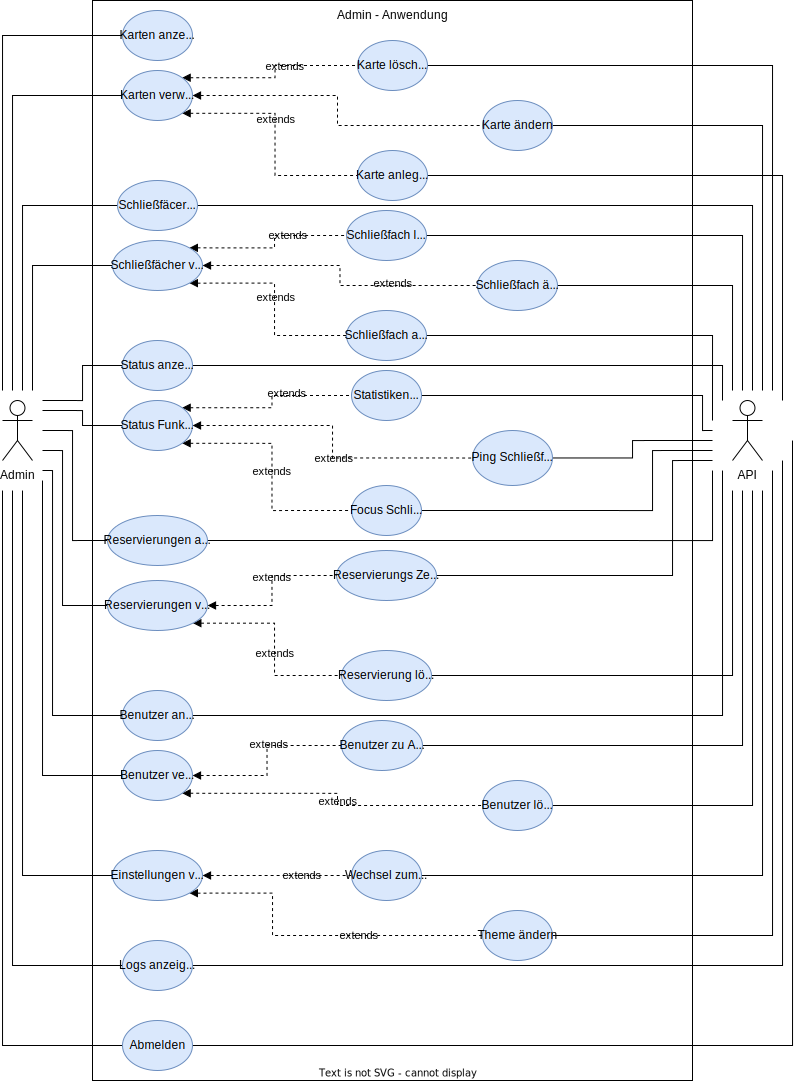
\includegraphics[width=0.92\textwidth]{FLUTTER/images/ZB/admin_use_case.png}
  \caption{Use-Case Admin-Sicht \cite{Flutter-Architektur-SVG}}
\end{figure} 
\newpage

\begin{figure}[h!]
  \centering
  \includegraphics[width=1\textwidth]{FLUTTER/images/GP/display-use-case.png}
  \caption{Use-Case Display-Sicht \cite{Flutter-Architektur-SVG}}
\end{figure} 

%\begin{figure}[h!]
 % \centering
 % \vspace{0.5cm}
 % \includegraphics[width=1\textwidth]{FLUTTER/images/GP/Use-Case.png}
 %   \caption{Use Case Diagramm der zu erstellenden Software}
%\end{figure}

\newpage

\section{Meilensteine}
\begin{itemize}
    \item 01.11.2022 Admin-Anwendung v1 abgeschlossen
    \item 01.11.2022 Client-Anwendung v1 abgeschlossen
    \item 01.11.2022 Display-Anwendung v1 abgeschlossen
    \item 01.11.2022 REST-API/DB v1 abgeschlossen
    
    \item 02.02.2023 Admin-Anwendung v2 abgeschlossen
    \item 02.02.2023 REST-API/DB v2 abgeschlossen
    \item 02.02.2023 Client-Anwendung v2 abgeschlossen
    \item 02.02.2023 Display-Anwendung v2 abgeschlossen

    \item 28.02.2023 Raspberry-API Kommunikation abgeschlossen
    \item 28.02.2023 Dokumentation abgeschlossen
    \item 30.04.2023 Abschluss Test durchgeführt 
\end{itemize}

%%%%%%%%%%%%%%%%%%%%%%%%%%%%%%%%%%5
\chapter{Eingesetzte Technologien der zentralen Schnittstelle \MjAnnotation{}}
{
\section{Go}\label{sec:tech:go}
Go ist eine für Systemprogrammierung (Dienste, Treiber, etc.) ausgelegte Programmiersprache mit kurzer und prägnanter Syntax. Entwickelt wurde die Sprache unteranderem von Robert Griesemer, Rob Pike und Ken Thompson (vgl. \cite{go:wiki}). Go bietet unteranderem automatische Speicherverwaltung, Typsicherheit, Closures, effiziente Nebenläufigkeitsmechanismen (goroutines). Go wird vor allem als serverseitige Programmiersprache für Webanwendungen und Microservices in Verbindung mit Virtualisierungsumgebungen wie Docker  eingesetzt.
\begin{wrapfigure}{r}{0.35\textwidth}
    \centering
    \includesvg[width=0.19\textwidth]{MJ/assets/Go_Logo_Blue.svg}
    \caption{Go Logo (vgl. \cite{GoLogoBlue})}
\end{wrapfigure}
Die Implementierung des Teilbereichs zur zentralen Schnittstelle des Systems (Kapitel \ref{ch-implementation}) des vorliegenden Projektes wurde ausschließlich in Go verfasst. Da Go eine relativ moderne Programmiersprache ist, und demnach weniger damit vertraut sind, werden in den folgenden Absätzen die wichtigsten Konzepte der Sprache anhand von Beispielen erklärt. Da sich speziell die Konzepte zum Thema Nebenläufigkeit in Go, doch sehr stark von beispielsweise Java oder ähnlichen Sprachen unterscheiden, werden diese hier etwas genauer erklärt um essentielle Teile der Implementierung zu verdeutlichen.\bigskip

\noindent
\textbf{Kurz zum Hintergrund:} \textit{Wieso Go? Wieso nicht Java oder Python?}\\
Der Hauptgrund für den Einsatz von Go als Programmiersprache eines beachtlichen Projektes, wie einer Diplomarbeit, war der Lernfaktor. Nach dem Einsatz von Go im Rahmen einiger privater Projekte, war Ich bereits mit der Sprache sowie dessen Eigenheiten vertraut. Die Alleinstellungsmerkmale (Goroutines, Concurrency, Channels) der Sprache und deren Ausführung, sind zum Großteil sehr elegant und clever gelöst. Vor allem der fehlende Overhead, verglichen mit Technologien wie Java, mit denen man ohne IDE und mehreren Frameworks nicht weit kommt, erleichtert den Entwicklungsprozess sehr. Die kompakte Syntax in Kombination mit statischen Typen ist ebenfalls sehr gut gelöst. Die erwähnten Mechanismen wie goroutines in Kombination mit Channels welche auf den ersten Blick mit Threads vergleichbar sind, erlauben es, anders über Probleme zum Thema Nebenläufigkeit nachzudenken und Lösungen zu finden, welche man mit herkömmlichen Technologien möglicherweise nicht erreicht hätte.\\
Zusammenfassend lässt sich sagen, dass die Beliebtheit von Go in Entwicklerkreisen definitiv gerechtfertigt ist.\bigskip 

\noindent
In den folgenden Abschnitten werden kurz die für die Implementierung relevanten Features der Sprache erklärt.
% \subsection{Relevante Features}
\subsection{Strukturen und Sichtbarkeit}
Ein \mono{struct} ist eine Sammlung von Datenfeldern, an welches Methoden angehängt werden können (vgl. \cite{go:spec:structs}). Structs sind vergleichbar mit Klassen in herkömmlichen Programmiersprachen wie Java. An ein solches Struct können Methoden angehängt werden, welche den Zustand der sich im struct befindlichen Datenfelder verändern.\bigskip

\noindent
\newpage
Hier ein Beispiel wie Structs in Kombination mit Methoden eingesetzt werden um Getter und Setter eines User-Objektes abzubilden. 
{\ColorfulCodeDisclaimer}
% \begin{minipage}[c]{\linewidth}
\begin{lstlisting}[style=goMono,caption={Struct in Kombination mit Methoden}]
type User struct {
    id        int    %\color{magenta}(1)%     
    Firstname string  
    Lastname  string 
}

func %\color{magenta}(2)% (u User) GetId() int {
    return u.id
}

func %\color{magenta}(3)% (u *User) SetId(id int) {
    u.id = id
}
\end{lstlisting}
% \end{minipage}
Im obigen Beispiel werden bereits einige Eigenheiten von Go demonstriert.\bigskip

\noindent
Go regelt die Sichtbarkeit von Variablen, Konstanten, Funktionen und Strukturen anders, manche meinen sogar eleganter, als beispielsweise Java. Es wird nicht jedes Element (Variablen, Funktionen, etc.) einzeln mit einem Sichtbarkeitsmodifizierer wie \mono{public} oder \mono{private} ausgestattet, sondern die Schreibweise des jeweiligen Elements wird beachtet. Elemente, welche mit kleinem Anfangsbuchstaben beginnen sind nur innerhalb der jeweiligen Übersetzungseinheit sichtbar (also innerhalb des \frqq{}\mono{package xyz}\flqq{}). Elemente, die mit großem Anfangsbuchstaben beginnen sind öffentlich sichtbar.\bigskip

\noindent
Mit diesem Hintergrundwissen ausgestattet sollte auch sofort ersichtlich sein wieso für das Attribut \mono{\color{magenta}(1)} \mono{id} Getter und Setter definiert werden müssen. Nun zu \mono{\color{magenta}(2)} und \mono{\color{magenta}(3)}. Dies sind Bespiele für Methoden, also Funktionen die an eine Struktur angehängt wurden und auf die inneren Attribute lesend oder schreibend, zugreifen können. In letzterer Aussage liegt auch gleich der Unterschied zwischen den beiden hervorgehobenen Punkten: lesend, technisch korrekt formuliert \textit{Call-By-Value} und schreibend, also \textit{Call-By-Reference}.  

\newpage
\subsubsection{Struct-Tags}
Datenfelder einer Struktur können mit Attributen ausgezeichnet werden, die von Bibliotheken und Frameworks genutzt werden um beispielweise den JSON-Namen eines Attributes zu definieren (vgl. \cite{go:spec:structs}).\\
Hier ein Bespiel wie \frqq{}struct-tags\flqq{} in Go eingesetzt werden um ein Objekt zu serialisieren.
\begin{lstlisting}[style=goRaw,caption={\centering Objekt \textit{User}, welches mit struct-tags annotiert wurde um die JSON-Serialisierung zu konfigurieren.}]
type User struct {
    ID        int     `json:"-"`
    Firstname string  `json:"my_firstname"`
    Lastname  string  `json:"my_lastname"`
    Skills    []Skill `json:"my_skills"`
}
\end{lstlisting}
Das obige Beispiel demonstriert, wie \frqq{}struct-tags\flqq{} also herkömmliche doppelte Hochkommas (\mono{"}) bzw. rückwärts geneigte Hochkommas (\mono{\`{}}) (engl. \textit{backticks}), dazu verwendet werden, Datenfelder im Struct mit Attributen zu versehen, welche in diesem Fall von dem JSON-Parser in der Standardbibliothek (über ein Reflection Interface im \frqq{}\mono{reflect}\flqq{} package) eingelesen werden. Eine mit \frqq{}\mono{json.Marshal}\frqq{} (vgl. \cite{go:pkg:json:marshal}) serialisierte Instanz der obigen Struktur könnte folgendermaßen aussehen:\\
\verb|{"my_firstname": "Max", "my_lastname": "Mustermann", "my_skills": ["mustern"]}|.\\
Wie erwartet werden die konfigurierten Felder richtig benannt, die \frqq{}Skills\frqq{} auch korrekt als JSON-Array serialisiert und das \mono{ID}-Feld wurde ignoriert da es in der Definition mit \verb|json:"-"| annotiert wurde. 

\subsection{Aufzählungen}
Aufzählungen, auch bekannt unter Enumerationen gruppieren ähnliche Attribute. Aufzählungen in Go funktionieren anders als in Java oder vergleichbaren Sprachen. In Go wird \mono{iota} verwendet um fortlaufende Aufzählungen zu generieren. \mono{iota} ist ein Zähler der standardmäßig bei 0 beginnt und nach jedem Element in der Aufzählung um 1 erhöht wird. Dieses Verhalten kann durch verschiedene Ausdrücke konfiguriert werden. Dieser Zähler wird nach jeder Aufzählung wieder auf 0 zurückgesetzt. Folgendes Beispiel, das eine Aufzählung von verschiedenen Automarken definiert, veranschaulicht das beschriebene Konzept.
\begin{lstlisting}[style=goMono,caption={Aufzählung von Automarken},label={lst:tech:go:enum:ex1}]
const (
    Jeep = iota + 1 %\color{magenta}(1)%
    _
    Audi     
    Mercedes
    Volkswagen
    LandRover
)
\end{lstlisting}
Der Vollständigkeit halber befindet sich im Anhang (siehe Abschnitt \ref{sec:apdx:extendedcode}) der vollständige Go-Code, welcher die im obigen Listing angegebene Ausgabe erzeugt.\\
Hier erfolgt nun eine kurze Erklärung, wie der obige Ausschnitt zu verstehen ist. Die mit \mono{\color{magenta}(1)} markierte Zeile im Listing ist die eigentliche Aufzählung. Hier wird \mono{iota}, eine ganzzahlige Konstante, verwendet um den sich innerhalb der Aufzählung \mono{( ... )} befindlichen Namen einen Wert zuzuordnen. Da \mono{\color{magenta}(1)} die einzige Zuweisung ist, wird diese für die restlichen Namen wiederholt. Nun wird \mono{iota} für jedes Auto um 1 erhöht sodass den Autos schlussendlich folgende Konstanten zugewiesen werden: \mono{Jeep}=1, \mono{Audi}=3, \mono{Mercedes}=4, \mono{Volkswagen}=5, \mono{LandRover}=6. Der \mono{\_} Indentifier steht immer für einen Namen der ignoriert wird, darum wird \mono{Audi} auch der Wert 3, statt 2, zugeordnet.

\subsection{Concurrency Patterns in Go}
\begin{tcolorbox}
\centering\textit{%
\frqq{}Do not communicate by sharing memory; instead, share memory by communicating.\flqq \cite{go:proverbs:concurrency} }
\end{tcolorbox}\bigskip
% https://go.dev/blog/codelab-share
\noindent
Concurrency, dt. Gleichzeitigkeit, also Prozesse welche gleichzeitig ausgeführt werden, sollten in Go dem oben genannten Ideal folgen: Kommunikation zwischen gleichzeitig ablaufenden Prozessen mittels Nachrichtenaustausch. Damit ist gemeint, dass Prozesse die gleichzeitig ablaufen (goroutines), sich über eine gemeinsame Schnittstelle (den Channels) austauschen und synchronisieren sollen anstatt eine im Speicher für alle Prozesse zugängliche, gemeinsame Datenstruktur oder Klasse zu bearbeiten.\bigskip

\noindent
Go stellt diese und weitere Bausteine, die auf diesen Konzepten aufbauen, bereits im Sprachkern bzw. in der Standardbibliothek bereit, sodass keine weiteren Frameworks oder Bibliotheken geladen werden müssen und stellt damit sicher, dass diese effizient und korrekt implementiert sind. In den folgenden Abschnitten werden die für die vorliegende Implementierung (siehe Abschnitt \ref{ch-implementation}) benötigten Konzepte anhand von Beispielen vorgestellt und näher erläutert sodass die weiteren, in der Implementierung benötigten Konzepte, einfacher zu verstehen sind.    

\subsubsection{Goroutines}
Go-routinen sind speichereffiziente Threads, die von der Go-Runtime verwaltet werden (vgl. \cite{go:goroutines}). Sobald eine Funktion mit dem Schlüsselwort \mono{go} vorangestellt wird, wird diese von der Runtime als Goroutine vermerkt und im Hintergrund ausgeführt. Im Vergleich zu Threads sind Goroutinen effizienter, sodass viele Goroutinen gleichzeitig laufen können. Der Programmierer muss sich über die Speicherverwaltung keine Gedanken machen, da dies von der Runtime übernommen wird.\\ Im folgenden Listing wird ein einfaches Beispiel dargestellt, das die Funktionsweise von Goroutinen veranschaulicht: 
\begin{lstlisting}[style=goMono,caption={Beispiel Goroutine},label={lst:go:sync:concurrency:ex1}]
func say(s string) {
	for i := 0; i < 5; i++ {
		time.Sleep(100 * time.Millisecond)
		fmt.Println(s)
	}
}

func main() {
	go say("world") %\color{magenta}(1)%
	say("hello")
}
\end{lstlisting}
Die Funktion \frqq{}\mono{say}\frqq{} wird auf zwei verschiedene Arten aufgerufen. Im ersten Aufruf als Goroutine \mono{\color{magenta}(1)} und im zweiten wird diese im Hauptprogramm (in der Haupt- bzw. Main-Goroutine) aufgerufen. Dabei ist anzumerken, dass das Programm beendet wird sobald das Hauptprogramm abgearbeitet wird, also sobald die Funktion \verb|say("hello")| fünf mal die Zeichenkette \frqq{}hello\flqq{} ausgegeben hat, auch wenn \verb|go say("world")| noch nicht fertig ist. Die Ausgabe auf der Konsole hängt davon ab welche Goroutine der Scheduler (das Programm, welches die Ausführung aller Goroutines verwaltet) zuerst ausführt. Folgende Ausgabe könnte auftreten:
\begin{lstlisting}[style=goMono,caption={Beispiel Goroutine},label={lst:go:sync:concurrency:ex1:output}]
hello
world
hello
world
world
hello
world
hello
hello
\end{lstlisting}
Die Goroutine \verb|go say("world")| konnte nicht vollständig beendet werden da das Hauptprogramm \mono{main()} davor bereits beendet wurde. In der Standardbibliothek befindet sich eine Lösung für dieses Problem. Um auf Goroutinen zu warten, welche noch nicht fertig sind, ohne das diese vom Hauptprogramm abrupt beendet werden, bietet Go eine sogenannte \mono{sync.WaitGroup} (vgl. \cite{go:waitgroup}). Dieser Typ befindet sich im \mono{sync} Paket und muss (zusätzlich zu dem Formatierungspaket \mono{fmt} und dem Paket zur Zeitverwaltung \mono{time}) importiert werden. 

\subsubsection{Synchronisation: \mono{sync.WaitGroup}}
Wie im obigen Abschnitt erläutert können WaitGroup's, welche zur Synchronisation dienen, dazu verwendet das in Listing \ref{lst:go:sync:concurrency:ex1:output} ersichtliche Problem zu beheben.\\
Im nachfolgenden Beispiel wird mit Hilfe einer WaitGroup sichergestellt dass die Goroutine \verb|go say("world")| aus Listing \ref{lst:go:sync:concurrency:ex1} vollständig abgearbeitet wird.

\begin{minipage}[c]{\linewidth}
\begin{lstlisting}[style=goMono,caption={Beispiel Goroutine: Synchronisation mittels \mono{sync.WaitGroup}}, label={lst:go:sync:concurrency:ex2}]
package main

import (
    "time"
    "fmt"
    "sync"
)

func main() {
    var wg sync.WaitGroup 

    wg.Add(1) %\color{magenta}(1)%
    go func() {
        say("world")
        wg.Done() %\color{magenta}(2)%
    }()
    
    say("hello")
    
    wg.Wait() %\color{magenta}(3)%
}
\end{lstlisting}
\end{minipage}
Die Funktion \frqq{}\mono{say}\flqq{} aus Listing \ref{lst:go:sync:concurrency:ex1} bleibt unverändert. Nur der Aufruf als Goroutine wird in eine anonyme Funktion die nun als Goroutine ausgeführt wird, verlagert. WaitGroup's haben einen internen Zähler \mono{\color{magenta}(1)}, der für die Anzahl der laufenden Goroutinen verwendet wird. Mit der Methode \mono{wg.Wait()} wird in diesem Fall die Terminierung des Hauptprogramms solange angehalten, bis dieser Zähler 0 ist. Ist dies der Fall gibt \mono{wg.Wait()} die Kontrolle an den Aufrufer zurück und beendet in diesem Fall das Programm. Der Zähler wird mit \mono{\color{magenta}(1)} um N, in diesem Fall um 1, inkrementiert und mit \mono{\color{magenta}(2)} um 1 dekrementiert. Es wird also solange gewartet \mono{\color{magenta}(3)} bis der Zähler von 1, wieder auf 0 gesetzt wird, was nur dann passiert wenn \frqq{}\verb|say("world")|\flqq{} vollständig ausgeführt wurde. Problem gelöst.  
\subsubsection{Channels}
Channels, also Kommunikationskanäle, sind das in Go primär verwendete Konzept um Daten zwischen den oben vorgestellen Goroutinen auszutauschen (vgl. \cite{go:channels}). Daten können mit dem \mono{<-} Operator auf einen Channel gesendet und davon gelesen werden. Folgendes Beispiel (vgl. \cite{go:channels}) veranschaulicht dieses Konzept.
\begin{lstlisting}[style=goMono,caption={Beispiel Channels},label={lst:go:sync:concurrency:ex3}]
package main

import "fmt"

func main() {
    messages := make(chan string) %\color{magenta}(1)%

    go func() { %\color{magenta}(2)%
        messages <- "ping" %\color{magenta}(3)%
    }()

    msg := <-messages %\color{magenta}(4)%
    fmt.Println(msg)
}
\end{lstlisting}
Go stellt die Funktion \mono{make}, die Instanzen von verschiedenen Typen wie Slices (vergleichbar mit Listen, etc.), Maps und eben auch Channels erzeugt, zur Verfügung. In \mono{\color{magenta}(1)} ist ein Beispiel für die Instanziierung eines Channels über welchen Zeichenketten also \mono{string}'s ausgetauscht werden können, angeführt. Der Name \mono{messages} ist nun eine Referenz auf diesen erzeugten Channel, der nun als Kommunikationsmedium für mehrere Goroutinen zur Verfügung steht. Um den Sachverhalt so einfach wie möglich zu halten, handelt es sich in diesem Beispiel aber nur um eine Goroutine. Die in \mono{\color{magenta}(2)} definierte Goroutine wird in Form einer anonymen Funktion definiert und danach sofort aufgerufen. Dieses Designpattern, dass anonyme Funktionen als Goroutinen ausgeführt werden, wird häufig verwendet, da, wie in diesem Beispiel ersichtlich die Goroutine so direkten Zugriff auf den Channel hat. Die Goroutine besteht nur aus einer Anweisung: \textit{sende die Zeichenkette \frqq{}ping\flqq{}} über den Channel \frqq{}messages\flqq{}, sodass diese von anderen Goroutinen gelesen werden kann. Nachrichten werden wie in \mono{\color{magenta}(3)} ersichtlich mit dem \mono{<-} Operator gesendet. In \mono{\color{magenta}(4)} wird mit demselben Operator wieder vom Channel gelesen. Jedoch ist nun der Channelname rechts vom Operator anstatt links, was anzeigt, dass nun vom Channel gelesen wird und das Ergebnis in der Variable \mono{msg} gespeichert wird.\bigskip

\noindent
\paragraph{Wie wird sichergestellt, das zum Zeitpunkt zu dem der Channel \mono{messages} ausgelesen wird \mono{\color{magenta}(4)}, bereits ein Wert vorhanden ist?} Der \mono{messages} Channel ist ein Beispiel für einen \textit{Unbuffered Channel}, also einen ungepufferten Channel. Dies bedeutet, dass Lese- und Schreiboperationen blockieren. Für das konkrete Beispiel bedeutet das, dass die Leseoperation \mono{\color{magenta}(4)}, solange die Ausführung des Programms blockiert, bis die einzige Schreiboperation \mono{\color{magenta}(3)} ausgeführt wurde.  Würde keine Goroutine auf den \mono{messages} Channel schreiben, aber trotzdem davon gelesen werden, würde das Programm zur Laufzeit mit folgendem Fehler abstürzen:\\ \mono{fatal error: all goroutines are asleep - deadlock!}. Wäre \mono{messages} ein \textit{Buffered Channel}, also ein Channel mit einer konstanten Pufferung, würde die obige Leseoperation nicht blockieren, solange der Channel nicht voll (der Puffer ist mit Nachrichten aufgefüllt) ist. Mehr Informationen zu \textit{Unbuffered Channels} finden sich in der offiziellen Dokumentation (vgl. \cite{go:tour:concurrency}).\\ 

\newpage
\subsubsection{Synchronisation: \mono{sync.Mutex}}\label{sec:tech:go:sync:mutex}
In diesem Abschnitt wird ein weiteres für die Implementierung relevantes Konzept vorgestellt. Ein Mutex sperrt den Zugriff auf einen bestimmten Programmabschnitt für gleichzeitig ablaufende Unterprogramme und gibt diesen, nachdem die Arbeit, die sequentiell ausgeführt werden muss, abgeschlossen ist, wieder frei. Ein Anwendungsfall für ein solches Schloss ist der Zugriff auf eine globale Variable, die von mehreren Goroutinen verändert wird. Generell sollte der Einsatz von globalen Variablen, die in parallel ablaufenden Prozessen verändert werden, eher vermieden werden, doch manchmal ist dies unumgänglich. Um diese Schreibzugriffe zu kontrollieren, kann ein solches Schloss eingesetzt werden. Die beiden Operationen eines Schlosses sind die \mono{.Lock()} und \mono{.Unlock()} Methoden. Im folgenden Beispiel wird dies veranschaulicht:

\begin{minipage}[c]{\linewidth}
\begin{lstlisting}[style=goMono,caption={Beispiel \mono{sync.Mutex}},label={lst:go:sync:concurrency:ex4}]
var lock *sync.Mutex = &sync.Mutex{} %\color{magenta}(1)%

func update(numberPtr *int) { %\color{magenta}(2)%
    for {
        lock.Lock() %\color{magenta}(3)%
        *numberPtr = rand.Intn(1000) %\color{magenta}(4)%
        lock.Unlock() %\color{magenta}(5)%
    }
}
func main() {
    var number int
    go update(&number) %\color{magenta}(6)%
    go update(&number)
}
\end{lstlisting}
\end{minipage}
Der Vollständigkeit halber befindet sich im Anhang (siehe Abschnitt \ref{sec:apdx:extendedcode}), der vollständige Go-Code, der den in diesem Abschnitt vorgestellten Sachverhalt abbildet. Hier wurden lediglich die wichtigsten Teile dargestellt um den Abschnitt kurz zu halten. Doch nun zur Erklärung des obigen Beispiels. In \mono{\color{magenta}(1)} wird ein Schloss definiert, sodass dies für die in \mono{\color{magenta}(2)} definierte Funktion, \mono{update}, welche einer Variable eine Zufallszahl \mono{\color{magenta}(4)} zuweist, zugänglich ist. Vor jedem Schreibzugriff, wird die mit der Funktion geteilten Referenz, \mono{numberPtr}, gesperrt \mono{\color{magenta}(3)}. Nach dem Schreibzugriff wird das Schloss wieder geöffnet \mono{\color{magenta}(5)}. Dies hat einen kontrollierten Zugriff auf den geteilten Speicherbereich zur Auswirkung. \textit{Hinweis}: So sollte natürlich nicht programmiert werden. Dieser Sachverhalt könnte viel effizienter über einen gemeinsamen Channel abgebildet werden.    

\newpage
\subsubsection{Synchronisation: \mono{sync.Cond}}
In diesem Abschnitt wird ein weiteres für die Implementierung relevantes Konzept vorgestellt. Dieser Typ dient dazu, die Benachrichtigung von, in Goroutinen stattfindenden Ereignissen zu erleichtern. Damit ist gemeint, dass man mit Hilfe dieses Typen, die Goroutine B, über ein in Goroutine A stattfindendes Ereignis, benachrichtigen kann. Dieser Typ dient hauptsächlich dazu den Code zu verkürzen und Concurrency-Fehler zu vermeiden die nur schwer nachvollziehbar sind, da dieses Ereignis- und Benachrichtigungssystem auch über Channels in Kombination mit Locks 
(Mutex, siehe Abschnitt \ref{sec:tech:go:sync:mutex} \nameref{sec:tech:go:sync:mutex}) gelöst werden kann.\\
Das nachfolgende Beispiel kombiniert die zuvor bereits vorgestellten Konzepte, \mono{sync.WaitGroup} und \mono{sync.Mutex}, um ein einfaches ereignisgesteuertes Begrüßungssystem abzubilden.
\begin{lstlisting}[style=goMono,caption={Kombination aus Concurrency Konzepten: Begrüßungssystem},label={lst:go:sync:concurrency:ex5}]
func main() {
    var wg sync.WaitGroup
    var cond *sync.Cond = sync.NewCond(&sync.Mutex{}) %\mono{\color{magenta}(9)}%
    
    people := []string{"Nick", "Alecia", "Madison", "Victor", "Travis"} %\mono{\color{magenta}(2)}%
    greetings := []string{} %\mono{\color{magenta}(3)}%
    
    wg.Add(1)
    go func() {
        cond.L.Lock()
        for len(greetings) != len(people) { %\mono{\color{magenta}(5)}%
            cond.Wait() %\mono{\color{magenta}(6)}%
        }
        for _, greeting := range greetings { %\mono{\color{magenta}(7)}%
            fmt.Println(greeting) %\mono{\color{magenta}(8)}%
        }
        cond.L.Unlock()
        wg.Done()
    }()
    
    for _, person := range people {
        cond.L.Lock()
        greetings = append(greetings, greet(person)) %\mono{\color{magenta}(1)}%
        cond.L.Unlock()
    }
    cond.Broadcast() %\mono{\color{magenta}(4)}%
    wg.Wait()
}
\end{lstlisting}
Wie oben erwähnt, kombiniert dieses Beispiel einige der bereits vorgestellten Concurrency Konzepte. Dieses Programm setzt ein einfaches Begrüßungssystem um. Zuerst \mono{\color{magenta}(1)} werden die Begrüßungen aus den gegebenen Namen \mono{\color{magenta}(2)} generiert und in einem Go-Slice (vergleichbar mit einer Liste) \mono{\color{magenta}(3)} abgespeichert. Sobald die Begrüßungen generiert sind sollen die Personen begrüßt werden. Die wartende Goroutine wird mit \mono{\color{magenta}(4)} \mono{Broadcast()} aufgeweckt und überprüft erneut ob die Bedingung, dass alle Begrüßungen generiert wurden (die Länge des \mono{greeting} Slice gleich der Länge des \mono{people} Slice ist) wirklich zutrifft \mono{\color{magenta}(5)} (es könnte ja sein, dass die Goroutine vom Scheduler aufgeweckt wurde, ohne dass die Bedingung zutrifft). Wenn nicht, wird weiter gewartet \mono{\color{magenta}(6)}. Ansonsten werden alle Personen begrüßt \mono{\color{magenta}(7)} (auf der Konsole ausgegeben) \mono{\color{magenta}(8)} und der WaitGroup-Zähler wird mit \mono{Done()} \mono{\color{magenta}(9)} um 1 verringert. Die eigentliche \mono{sync.Cond} Deklaration bekommt im Konstruktor ein \mono{sync.Mutex} Lock übergeben, sodass auf die mit den Goroutinen geteilten Datenstrukturen atomar (also zu jedem Zeitpunkt nur 1 Goroutine), zugegriffen werden kann. Das \mono{sync.Cond} Paket stellt ausserdem noch eine \mono{Signal()} Methode bereit, um nur \textit{eine} Goroutine aufzuwecken, anstatt mit \mono{Broadcast()} alle wartenden Goroutinen aufzuwecken. In diesem Beispiel bleibt das aber gleich, da sowieso nur 1 Goroutine auf ein Signal wartet.\\
Wie gehabt befindet sich das vollständig funktionierende Beispiel im Anhang (siehe Abschnitt \ref{sec:apdx:extendedcode}).

% \subsection{Verwaltung von Abhängigkeiten}
% go-get ...

% \subsection{Generator-Anweisungen}
% ...

\newpage
Docker ist ein Werkzeug, um Software, in einer konfigurierbaren und abgeschotteten Umgebung betreiben zu können (vgl. \cite{wiki:docker}). Docker wird gerne in Verbindung mit Go (siehe Abschnitt \ref{sec:tech:go}) eingesetzt, da Go-Anwendungen auf ein einziges, ausführbares Programm kompiliert werden und daher wenige Abhängigkeiten nach aussen haben.  
\section{Docker}\label{sec:tech:docker}
\begin{figure}[h!] % {r}{0.375\textwidth}
    \centering
    \includesvg[width=0.21\textwidth]{MJ/assets/Docker_logo.svg}
    \caption{Docker Logo (vgl. \cite{DockerLogo})}
\end{figure} 
In der nachfolgenden Implementierung wurde Docker verwendet, um das gesamte System zu containerisieren. Docker kümmert sich um alle Abhängigkeiten und stellt diese den Anwendern im zugehörigen Docker-Hub, zur Verfügung. Dies schränkt den Verwaltungsaufwand einer Software erheblich ein.

\section{MySQL}
MySQL ist ein frei verfügbares, relationales Datenbankverwaltungssystem (vgl. \cite{wiki:mysql}). Damit ist gemeint, dass Tabellen ein \textit{Schema} also eine Struktur haben. Tabellen können über Relationen, in Beziehung zueinander stehen. In Beziehung zueinander stehende Tabellen weisen eine Fremdschlüsselbeziehung auf, die durch ein Foreign-Key Contraint definiert wird. Eine solche Fremdschlüssel Einschränkung definiert, anhand welcher Schlüssel die Tabellen miteinander verbunden sind. 
\begin{figure}[h!]
    \centering
    \includesvg[width=0.19\textwidth]{MJ/assets/MySQL_logo.svg}
    \caption{MySQL Logo (vgl. \cite{MySqlLogo})}
\end{figure} 

\newpage
\section{GORM}\label{sec:theory:orm}
\newacronym{orm}{ORM}{Object Relational Mapper}
% GORM ist ein \acrlong{orm}-Framework für Go. Theoretische Informationen zu \acrlong{orm}'s finden sich im Abschnitt \ref{sec:theory:orm} (\nameref{sec:theory:orm}). Nähere Informationen zu der Programmiersprache Go finden sich im Abschnitt \ref{sec:tech:go} (\nameref{sec:tech:go}). Die Integration von GORM findet hauptsächlich anhand von sog. `struct tags' statt. Diese ist grundsätzlich ein Feature welches Go selbst unterstützt und von GORM ausnutzt wird. 
GORM ist ein \acrlong{orm}-Framework für Go. Nähere Informationen zu der Programmiersprache Go finden sich im Abschnitt \ref{sec:tech:go} (\nameref{sec:tech:go}). Die Integration von GORM findet hauptsächlich anhand von sog. \frqq{}struct tags\frqq{} statt. Diese sind grundsätzlich ein Feature, das Go selbst unterstützt und von GORM ausnutzt wird. 
\subsection{Demonstration anhand eines Beispiels}
Im folgenden Abschnitt wird die Funktionalität des oben erläuterten \acrshort{orm}-Frameworks, \textit{GORM}, anhand eines Beispiels dargestellt. Das folgende Beispiel beschränkt sich lediglich auf die Definition einzelner Objekte, welche von GORM in ein lauffähiges (MySQL) Datenbankschema übersetzt werden. Das Beispiel soll einige Features von GORM demonstrieren, die sich auch in ähnlicher Form in der vorliegenden Implementation wieder finden.
\begin{lstlisting}[style=goMono,caption={GORM Demonstration anhand eines konkreten Beispiels},label={lst:tech:gorm:ex1}]
type Office struct {
  OfficeID   uint     `gorm:"primaryKey"`                    
  Department string   `gorm:"default:'IT'"` %\color{magenta}(4)%
  Workers    []Worker `gorm:"foreignKey:SSN"` %\color{magenta}(1)%
}

type Worker struct {
  SSN       uint      `gorm:"primaryKey"`     
  FirstName string    `gorm:"type:varchar(32)"` 
  LastName  string    `gorm:"type:varchar(32)"`
  OfficeID  uint      `gorm:"foreignKey:OfficeID"` %\color{magenta}(2)%
  Office    Office %\color{magenta}(3)%
}
\end{lstlisting}
Das obige Beispiel demonstriert, wie GORM die Struct-Tags (nähere Informationen dazu im Abschnitt \ref{sec:tech:go} \nameref{sec:tech:go}) der einzelnen Datenfelder der Objekte interpretiert, um so das resultierende Datenbankschema zu konfigurieren. 
Die Beziehung zwischen einem Office, das mehrere Arbeiter beinhaltet, \mono{\color{magenta}(1)} wird auch bereits korrekt abgebildet. GORM verwendet dazu die Reflection Schnittstelle, welche die Go-Runtime zur Verfügung stellt und erstellt die 1-N Fremdschlüsselbeziehung zwischen \textit{Office} und \textit{Worker} da es sich bei dem \mono{Workers} Feld im Office um ein Go-Slice, vergleichbar mit einem dynamischen Array bzw. einer \mono{List<Worker>} in Java, handelt. Weiters wird die \mono{foreignKey} Annotation ausgelesen, um GORM mitzuteilen, über welche Spalte die Beziehung zu definieren ist. Damit auch der \textit{Worker} über seine Zugehörigkeit zu einem \textit{Office} Bescheid weiß, wird auch hier \mono{\color{magenta}(2)}, \mono{\color{magenta}(3)} eine Beziehung zum \textit{Office} definiert.\\
Abschließend wird im Beispiel noch die Definition von Default-Constraints demonstriert \mono{\color{magenta}(4)}: \textit{Office}'s gehören standardmäßig zur IT-Abteilung. GORM generiert aus obigem Go-Code folgendes Datenbankmodell.\bigskip
\begin{figure}[h!]
    \centering
    \makebox[\textwidth][c]{\includegraphics[width=1.15\textwidth]{MJ/assets/schema_office_example_cropped.svg.png}}
    \caption{von GORM aus Listing \ref{lst:tech:gorm:ex1} generiertes Datenbankmodell}
    \label{img:tech:gorm:schema:ex1}
\end{figure}

\newpage
\noindent
In der obigen Abbildung wird auch bereits das Standardverhalten von GORM ersichtlich. GORM hat den Go-Datentyp \mono{string}, der im \mono{Department} nicht genauer definiert wurde als \mono{varchar(191)} übersetzt. Um solche, eher weniger optimalen Abbildungen von Go auf das Datenbankmodell zu vermeiden, sollten Datentypen und Constraints immer explizit definiert werden um Konflikte zu vermeiden. 
Der Vollständigkeit halber befindet sich im Anhang (siehe Abschnitt \ref{sec:apdx:extendedcode}) der komplette Go-Code, der das in Abbildung \ref{img:tech:gorm:schema:ex1} veranschaulichte Datenbankmodell generiert.

\section{Gorilla}\label{sec:tech:gorilla}
Gorilla ist ein für die vorliegende Implementierung zum Einsatz kommendes Go-Toolkit, also eine Sammlung mehrerer Komponenten, mit der schnell und einfach Web Anwendungen entwickelt werden können (vgl. \cite{go:gorilla}). Gorilla beinhaltet Komponenten, unteranderem einen HTTP Multiplexer \mono{gorilla/mux}, der die eingehenden und ausgehenden HTTP-Anfragen an die richtigen Endpunkt-Handler weiterleitet. Eine weitere wichtige Komponente ist die Websocket-Bibliothek \mono{gorilla/websocket}, die ebenfalls für die vorliegende Implementierung zum Einsatz kommt. Schließlich wurde noch die Gorilla-Middleware Bibliothek \mono{gorilla/handlers}, in Kombination mit \textit{Meridian}, dem eigens für dieses Projekt entwickelte Middleware-Framework, eingesetzt.    

% \newpage
% \section{Technologien zur Dokumentation des Projektes}

% % \subsection{Swagger} 
% % (OpenAPI)

% \subsection{Textsatzsystem \LaTeX{}}
% Im Rahmen der vorliegenden Arbeit habe Ich mich umfassend mit dem Textsatzsystem \TeX{} und dessen erfolgreicher Erweiterung, \LaTeX{},  befasst. Auf der Suche nach einem vernünftigen System, um sauber und möglichst effizient, schöne Dokumente zu verfassen, experimentierte Ich mit einigen Systemen wie \textit{groff}, \textit{Markdown} und \textit{Con\TeX{}t}. Markdown zu wenige Features (ohnehin nicht dazu gedacht),  (Ablehnung der Profit und Consumer-orientierten Microsoft Philiosophie sowie zu kompliziert zu Verwenden)\\
% MS Word vs TeX: WYSIWYG vs WYSIWYAF (https://de.wikipedia.org/wiki/WYSIWYG)\\
% dokumentationsprojekt-struktur\\
% verwendete environments um text zu formatieren bzw. grafiken zu generieren\\

}

\chapter{Theoretischer Hintergrund zur zentralen Schnittstelle \MjAnnotation{}}
{
% \section{Hinweis für LeserInnen}
\section{Verbindungsorientierung: TCP}\label{sec:theory:tcp}
\newacronym{tcp}{TCP}{Transmission Control Protocol}
\newacronym{osi}{OSI}{Open Systems Interconnection model}
\newacronym{ack}{ACK}{Acknowledge, dt. Bestätigung, Anerkennung}
Wie kann sichergestellt werden, dass die gesendeten Daten auch wirklich ankommen? Hier wird kurz anhand des TCP Protokolls erklärt, das in der vorliegenden Implementierung zum Einsatz kam, warum man in den allermeisten Fällen davon ausgehen kann, dass die gesendeten Daten, sprich Anweisungen vom Server eine Schlüsselkarte aus dem Schließfach zu befördern oder aber das Kommando, eine Karte aus der Datenbank zu entfernen, auch wirklich beim richtigen Empfänger, korrekt ankommen.
\begin{wrapfigure}{l}{0.65\textwidth}
\centering
\includesvg[width=0.625\textwidth,inkscapelatex=false,pretex=\escapeus]{MJ/assets/iso-schichten.svg}
\caption{\centering Datenverkehr zwischen zwei Systemen gemäß dem OSI Schichtenmodell (vgl. \cite{osi-layers})}
\label{img:osi-layers}
\end{wrapfigure}
Nachfolgend wird kurz die Funktionsweise von TCP, als verbindungsorientiertes Transportprotokoll innerhalb des OSI-Schichtenmodells erläutert und wie TCP die Datenintegrität gewährleistet. Die Transportschicht, des in Abbildung \ref{img:osi-layers} dargestellten \acrshort{osi} Schichtenmodells sorgt dafür, dass die Kommunikation zwischen den Endgeräten gewährleistet ist. Dabei ordnet TCP die an den Rechner ankommenden Datenströme in sogenannte \textit{Ports}, die unterschiedlichen Diensten zugeordnet sind: 80 für HTTP, 443 für HTTPS, 1884 für MQTT mit Authentifizierung, 22 für die Secure Shell etc. TCP teilt den zu übertragenden Datenstrom in Pakete auf, wobei ein Endpunkt immer aus einer IP-Addresse der darunterliegenden Vermittlungsschicht sowie eines Ports besteht. Sobald der Empfänger das Teilpaket erhalten hat, bestätigt dieser den Empfang mit einem TCP-\acrshort{ack}, also einer Nachricht an den Sender dass das Teilpaket (auch Segment genannt) angekommen ist. Wird der Empfang eines Segments vom Empfänger nicht bestätigt, sendet der Sender, den möglicherweise verloren gegangenen Teil des Paketes, nachdem die restlichen Segmente übertragen wurden, nochmals. Die Reihenfolge der gesendeten Segmente ist nicht von Bedeutung da diese vom Sender indiziert werden, sodass der Empfänger diese nach dem vollständigen Empfang wieder, in der richtigen Reihenfolge, zusammensetzen kann. Darüber hinaus stellt TCP auch einen kontrollierten Verbindungsaufbau, den sogenannten TCP-Handshake, der dafür sorgt, dass sowohl Sender, als auch Empfänger bereit sind, Daten miteinander auszutauschen, sowie einen kontrollierten Verbindungsabbau, den TCP-Teardown, welcher dem Empfänger anzeigt, dass vom Sender keine Daten mehr kommen, sicher (vgl. \cite{wiki:tcp:handshake}, \cite{wiki:tcp:teardown}).\bigskip

\noindent
Nachdem für die vorliegende Implementierung TCP als Transportprotokoll verwendet wurde, ist davon auszugehen dass die zwischen den Schnittstellen ausgetauschten Daten auch bei den richtigen Empfängern, in der richtigen Reihenfolge und mit garantierter Datenintegrität, ankommen.   

\newpage
\section{HTTP}\label{sec:theory:http}
\newacronym{http}{HTTP}{Hypertext Transfer Protocol}
Das \acrlong{http} ist ein sich im \acrshort{osi}-Schichtenmodell auf Schicht 7 befindliches Anwendungsprotokoll (siehe Abbildung \ref{img:osi-layers}), das zum Austausch von Daten, vor allem im Internet, verwendet wird, um die Kommunikation zwischen Client und Server zu standardisieren. Jede HTTP Nachricht besteht aus zwei Teilen: dem Header und dem Body. Im Header, also im Kopf der Nachricht, stehen Informationen über den eigentlichen Inhalt wie z.B.: Typ (Reiner Text, JSON, XML, etc.), Nachrichtenlänge, Kodierung (UTF-8, UTF-16 etc.). Dieser Header werden als Key-Value Paare formuliert und können auch selbst definiert werden, solange diese mit \frqq{}\mono{X-}\flqq{} beginnen. Im Body der HTTP Nachricht befinden sich die eigentlichen Daten die übertragen werden sollen. Der Header ist standardmäßig vom Body mit zwei Zeilenumbrüchen \frqq{}\mono{\textbackslash{}r\textbackslash{}n\textbackslash{}r\textbackslash{}n}\flqq{} getrennt. HTTP ist ein zustandsloses Protokoll. Damit ist gemeint, dass HTTP Nachrichten standardmäßig unabhängig voneinander sind und daher keinen Bezug zueinander haben: \textit{Anfrage A} und \textit{Anfrage B} wissen nichts voneinander, und nehmen keinen Einfluss aufeinander. Möglichkeiten, um diese Zustandslosigkeit von HTTP zu umgehen, sind beispielsweise Cookies (Daten, die lokal am Client gespeichert werden und die der Browser automatisch im HTTP-Header bei jeder Anfrage an den Server sendet) oder Sessions (Daten über einen Client werden am Server gespeichert; der Server unterscheidet Clients anhand von eindeutigen Identifiers in Form von Cookies: Session-Cookie).

\subsection{Methoden}
\newacronym{uri}{URI}{Unique Resource Identifier}
Jede HTTP Anfrage (auch \textit{Request} genannt) hat eine Methode. Eine Methode gibt an, wie die Anfrage vom Server zu interpretieren ist. In diesem Abschnitt werden die für die Implementierung benötigten Methoden erklärt.
\begin{description}\setlength\itemsep{1.5em}
\item[\mono{GET}] Mit dieser Methode signalisiert der Client, dass dieser Daten, welcher der Server an dem angegebenen Endpunkt zur Verfügung stellt, herunterladen möchte. 
\item[\mono{HEAD}] Sendet der Client diese Methode an den Server, interpretiert der Server diese wie ein \mono{GET}. Der Server sendet jedoch nur die Header, ohne den eigentlichen Inhalt zurück. Diese Methode kann vom Client verwendet werden um den Inhaltstyp (Content-Type) der angeforderten Ressource zu überprüfen, ohne den Inhalt herunterladen zu müssen.
\item[\mono{OPTIONS}] Gibt die vom Server unterstützten Methoden im \mono{Allow} Header zurück (vgl. \cite{sec:theory:http:method:options}).
\item[\mono{POST}] Mit dieser Methode signalisiert der Client, dass dieser Daten an den Server übermitteln möchte. Die zu übermittelnden Daten können sich entweder in Form von Argumenten in der \acrshort{uri}\\ (\mono{http://example.com/upload?name=myPicture.png\&width=100\&height=200}),\\ im Pfad der \acrshort{uri}\\ (\mono{http://example.com/upload/name/myPicture.png/width/100/height/200}) oder im Body der HTTP Anfrage befinden\\(\mono{\{"name":"myPicture.png","width":100,"height":200\}}).    
\item[\mono{PUT}] Diese Methode ist der \mono{POST} Methode sehr ähnlich. Der Unterschied liegt in der Definition im Standard. \mono{PUT} soll laut Definition, vom Server so interpretiert werden, dass die Auswirkungen der Anfrage keine \textit{Nebeneffekte} haben. Damit ist gemeint dass die Anfrage mehrmals aufgerufen werden kann und diese immer dieselbe Auswirkung erzielt (Foto auf den Server hochladen, etc). Dieses Verhalten wird auch \textit{idempotent} genannt (vgl. \cite{sec:theory:http:method:put}).
\item[\mono{DELETE}] Diese Methode signalisiert dem Server dass die vom Client spezifizierte Ressource gelöscht werden soll.
\end{description}

\subsection{Response Codes}
Teil der Antwort des Servers auf eine Anfrage vom Client ist der Rückgabewert. Mit diesem kann der Client Rückschlüsse auf den Erfolg seiner Anfrage ziehen. Einige wichtige Gruppen von Rückgabecodes sind:
{
\setlist{nolistsep}
\begin{description}[noitemsep] 
\item[1xx] Informationen
    \begin{description}[noitemsep] 
        \item[\textit{101 Switching Protocols}] Die TCP Verbindung wird nun für ein anderes Protkoll verwendet (z.B.: Websockets)
        \item[\ldots]
    \end{description}

\item[2xx] Erfolgreich
    \begin{description}[noitemsep] 
        \item[\textit{200 OK}] Anfrage war erfolgreich
        \item[\ldots]
    \end{description}
    
\item[4xx] Fehlerhafte Anfragen des Clients
    \begin{description}[noitemsep] 
        \item[\textit{400 Bad Request}] Fehlerhafte Formulierung einer Anfrage
        \item[\textit{401 Unauthorized}] Client ist nicht berechtigt auf die spezifizierte Ressource zuzugreifen
        \item[\textit{404 Not found}] Die spezifizierte Ressource wurde nicht gefunden
        \item[\ldots]
    \end{description}
    
\item[5xx] Serverfehler
    \begin{description}[noitemsep] 
        \item[\textit{500 Internal Server Error}] Fehler auf der Seite des Servers ist aufgetreten 
        \item[\ldots]
    \end{description}
\end{description}
}

\subsection{Authentifizierung}
HTTP stellt Authentifizierung, also die Überprüfung ob ein Client berechtigt ist auf eine gesicherte Ressource zuzugreifen, in Form von unterschiedlichen Mechanismen bereit.

\subsubsection{Basic-Authentication}
Die einfachste, aber eine nicht sehr sichere (und mittlerweile auch schon veralterte) Form der Authentifizierung ist die \textit{Basic-Authentication}: Der Client sendet seine Zugangsdaten (beispielsweise Benutzername und Passwort) in Base64-Kodierter Form an den Server (vgl. \cite{wiki:base64}). Der Server dekodiert die Zeichenfolge und überprüft ob der Benutzer berechtigt ist auf die gegebene Ressource zuzugreifen. Da die Base64-Kodierung der Zugangsdaten im Grunde nichts weiter als eine Verschleierung im Gegensatz zu einer Verschlüsselung ist, eignet sich dieser Ansatz nicht für sensible Daten wie Passwörter.\bigskip  

\noindent
Sicherere Alternativen zur Basic-Authentication, um beispielsweise Clients mit Zugangsdaten zu authorisieren, stellt z.B. die \textit{Digest-Authentication} dar. Die Zugangsdaten können damit, sofern eine kryptografisch sichere Hashfunktion verwendet wurde, nicht mehr ohne weiteres rekonstrukiert werden (vgl. \cite{wiki:http:auth:digest}).

\subsubsection{Bearer-Authentication}
Für die Implementierung der HTTP Schnittstelle (\nameref{sec:centralAPI}) wurde das sogenannte \textit{Bearer} Authentifizierungsschema verwendet, um die dort näher beschriebenen Ressourcen nur für berechtigte Benutzer zur Verfügung zu stellen. Nähere Erklärungen, um welche Ressourcen es sich handelt, werden dort beschrieben. Hier wird lediglich der theoretische Hintergrund zum genannten Schema kurz erläutert.\bigskip

\noindent
\textit{Bearer}, zu deutsch \textit{Träger} oder \textit{Inhaber}, ist die Authentifizierung mittels einer vom Server auf Basis von Benutzerdaten generierten Zeichenfolge (auch \textit{Token}, genauer \textit{Bearer}-Token genannt). Der Client sendet die vom Server geforderten Zugangsdaten, entweder in Klartext oder bereits in einer vom Server akzeptierten verschlüsselten bzw. kodierten Form. Der Server antwortet mit einem Token. Der Client übergibt nun diesen Token im \mono{Authorization: Bearer <TOKEN>} Header der gesicherten Ressource um darauf zugreifen zu können. Der Vorteil dieses Schemas ist die erhöhte Sicherheit der Zugangsdaten des Benutzers: diese müssen dem Server nur 1x (über eine meist ohnehin bereits verschlüsselte HTTPS Verbindung) übertragen werden. Jedoch kann man die Token-Authentifizierung noch etwas weiterführen. In Kombination mit JWT (siehe Abschnitt \ref{sec:theory:jwt} \nameref{sec:theory:jwt}) können Informationen in dem vom Server generierten Token in Form eines JSON-Objektes gespeichert werden. Diese Kombination aus Bearer-Authentifizierung und JWT's kam auch in der vorliegenden Implementation zum Einsatz. 

\subsection{Beispiele zu HTTP-Anfragen}
\newacronym{cli}{CLI}{command-line interface (dt. Kommandozeile)}
Im folgenden Abschnitt finden sich nun einige Beispiele zu HTTP Anfragen (\textit{Request}), sowie mögliche Antworten (\textit{Response}) welche die oben beschriebene Funktionsweise des HTTP Protokolls verdeutlichen sollen. Dies sind Beispiele für Anfragen, welche ein Browser (Chrome, Firefox, etc.) beim üblichen Surfen im Netz in rauen Mengen, an viele verschiedene Server sendet.\bigskip

\noindent
Kurz zum Aufbau der folgenden Beispiele: Es wurde ein lokaler Webserver auf dem Port 8085 gestartet, der eine einfache HTML-Datei im Basispfad hat:\\\mono{python3 -m http.server 8085 -{}-bind 127.0.0.1 -{}-directory .} .\\ Anfragen auf diesen Endpunkt wurden mit \mono{ngrep} (vgl. \cite{wiki:ngrep}), einem Paket Analysierungstool (vgl. \cite{wiki:packet-analyzer}) überwacht, sodass diese auf der Kommandozeile ausgegeben werden.\\ Ngrep ist ein sehr umfangreiches Tool mit vielen Funktionen. Für dieses Beispiel wurden lediglich einige Filter verwendet sodass nur HTTP Pakete auf Port 8085 auf dem \textit{loopback}-Interface, also \textit{localhost} (127.0.0.1) überwacht werden. Dies wurde mit folgendem Kommando erzielt: \mono{sudo ngrep -q 'HTTP' 'tcp' 'port 8085' -d lo}. 
Danach wurde die unten stehende Anfrage mit \mono{curl}, einem \acrshort{cli}-Tool um Daten in verschiedenen Protokollen im Netzwerk auszutauschen, folgendermaßen generiert:\\ \mono{curl -X GET http://127.0.0.1:8085}.
\newpage
\noindent
\ColorfulCodeDisclaimer{}\\
Das folgende Beispiel veranschaulicht eine GET-Anfrage an einen lokalen Webserver.
\begin{lstlisting}[style=goMono,caption={Bespiel 1: Demonstration der GET-Methode},label={lst:http:ex1}]
GET / HTTP/1.1           %\color{magenta}(1)%
Host: 127.0.0.1:8085     %\color{magenta}(2)%
User-Agent: curl/7.81.0  %\color{magenta}(3)%
Accept: */*              %\color{magenta}(4)%

%\color{magenta}(5)%
\end{lstlisting}
In der ersten Zeile \mono{\color{magenta}(1)} präsentiert sich bereits der wichtigste Teil der Anfrage. Die Methode (GET), gefolgt von der vom Client geforderten Ressource \frqq{}/\flqq{} (viele Webserver verstehen einen leeren Slash als \mono{/index.html}). Beendet wird \mono{\color{magenta}(1)} mit der vom Client unterstützten HTTP Version. Die folgenden Zeilen, \mono{\color{magenta}(1)}, \mono{\color{magenta}(2)} und \mono{\color{magenta}(3)} sind Beispiele für HTTP-Header. \mono{Host} gibt die Zieladresse des Servers an (in diesem Fall ein lokaler Webserver). Der \mono{User-Agent} identifiziert den Client (Software, welche die Request veranlasst samt Version). \mono{Accept} teilt dem Server mit, welche Inhaltstypen der Client gerne als Antwort auf seine Anfrage hätte. In diesem Fall akzeptiert der Client alles was der Server zurück gibt. \mono{\color{magenta}(5)} stellt den Anfang des HTTP-Body's und das Ende des Headers dar. Da der Client dem Server aber keine weiteren Daten mitgegeben hat, ist der Body leer.\bigskip

\noindent
Hier ein Beispiel wie eine erfolgreiche Antwort zu der obigen Anfrage aussehen könnte.
\begin{lstlisting}[style=goMono,caption={Bespiel 2: Erfolgreiche Anwort},label={lst:http:ex2}]
HTTP/1.0 200 OK                              %\color{magenta}(1)%
Server: SimpleHTTP/0.6 Python/3.10.6         %\color{magenta}(2)%
Date: Mon, 13 Feb 2023 23:57:29 GMT
Content-type: text/html                      %\color{magenta}(3)%
Content-Length: 7
Last-Modified: Mon, 13 Feb 2023 23:06:45 GMT
                                            
<html>                                       %\color{magenta}(4)%
<body>hello!</body>
</html>
\end{lstlisting} 
Anhand des Response Code in der ersten Zeile \mono{\color{magenta}(1)} ist erneut klar ersichtlich, dass es sich hier um eine Antwort des Servers handelt. Der Server identifiziert sich ebensfalls \mono{\color{magenta}(2)}, analog zum User-Agent der Anfrage. Als Content-Type \mono{\color{magenta}(3)}, also den Typ des Inhaltes im Body, sendet der Server HTML. Der Server beendet den Header mit \frqq{}\mono{\textbackslash{}r\textbackslash{}n\textbackslash{}r\textbackslash{}n}\flqq{} und sendet den vom Client angeforderten Inhalt der \mono{/} Resource. Dies ist der Inhalt, welcher im Browserfenster grafisch dargestellt werden würde. 

\section{Websockets}\label{sec:theory:ws}
Mit Hilfe des auf TCP (siehe Abschnitt \ref{sec:theory:tcp}) aufbauenden, \textit{Websocket} Protokolls können zwei Endpunkte miteinander in beiden Richtungen miteinander kommunizieren (vgl. \cite{src:ionos:websocket}). Es können auch HTTP-Verbindungen zu einer Websocket-Verbindung aufgewertet werden, um einen kontinuierlichen Datenaustausch zwischen Client und Server, der in beiden Richtungen funktioniert, umzusetzen. Dies wurde in der vorliegenden Implementierung so umgesetzt. Unterstützt ein HTTP Endpunkt die Aufwertung einer Verbindung auf eine Websocket-Verbindung, antwortet der Server dem Client mit dem Status-Code 101. Dieser steht in der HTTP-Spezifikation für einen Protokollwechsel. Der Server wechselt also vom HTTP Protokoll auf das Websocket Protokoll. Akzeptiert der Client, die vom Server angebotene Verbindung, ist die beidseitige Kommunikation hergestellt. Die nun bestehende Verbindung zwischen den beiden Endpunkten, kann als nahezu Echtzeit Transfer, genutzt werden (vgl. \cite{rfc:websocket})

\section{MQTT}\label{sec:theory:mqtt}
\newacronym{mqtt}{MQTT}{Message Queueing Telemetry Transport}
\acrshort{mqtt} ist ein Protokoll, das vor allem im \textit{Internet-of-Things} Raum, wie Smart-Home-Systemen, aufgrund seiner Einfachheit, große Anwendung findet (vgl. \cite{src:therory:mqtt}). Das Protkoll ist auf Basis einer zentralisierten Architektur aufgebaut. Der \textit{Broker}, also die Komponente, die den Nachrichten-Austausch zwischen verbundenen Clients koordiniert, kategorisiert diese Nachrichtenkanäle in sogenannte Topics. Zwei Clients können über ein gemeinsames Topic miteinander kommunizieren.   
\begin{figure}[h!]
    \centering
    \includesvg[width=0.19\textwidth]{MJ/assets/Mqtt_logo.svg}
    \caption{MQTT Logo (vgl. \cite{MqttLogo})}
\end{figure}
Der Broker dient als Schnittstelle zwischen den Clients. Dieser leitet die auf einem Topic empfangene Nachricht an alle Teilnehmer des Topics weiter. Wartet ein Client auf eingehende Nachrichten auf einem Topic so ist dieser \textit{subscribed}. Veröffentlicht ein Client, Nachrichten auf einem Topic so gilt dieser als \textit{Publisher}, wobei auch dieser auf andere Topics \textit{subscribed} sein kann. 

\section{Representational State Transfer}\label{sec:theory:rest}
\newacronym{rest}{REST}{Representational State Transfer}
\newacronym{restful}{RESTful}{Eine Schnittstelle welches der \acrshort{rest}-Spezifikation genügt.}
REST, \acrlong{rest}, ist ein auf HTTP aufbauender Architekturstil für Webdienste. Eine API wird dann \acrshort{restful} genannt, wenn diese die folgenden Kriterien erfüllt (vgl. \cite{src:redhat:rest}).
\begin{description}
\item[Ressourcen orientiert] Die vom Server zu bearbeitenden Objekte werden als Ressourcen betrachtet mit denen interagiert werden kann. Konkret, sind dies Karten, Benutzer, Schließfächer und Reservierungen.
\item[Einheitliche Schnittstelle zum System] Die über HTTP zur Verfügung gestellte Schnittstelle ist über verschiedene HTTP-Methoden (GET, POST, PUT, DELETE) erreichbar.
\item[Zustandslos] Anfragen verschiedener Clients sind unabhängig voneinander. 
\item[Client-Server Architektur] REST ist ein Client-Server Prinzip: Der Server beantwortet die Anfragen des Clients.
\end{description}
Im Zuge der Implementierung wird erläutert, ob und wie die Benutzer-Schnittstelle diese Anforderungen erfüllt und warum.

\section{JavaScript Object Notation}\label{sec:theory:json}
\newacronym{json}{JSON}{JavaScript Object Notation}
\acrshort{json} ist ein Datenformat (vgl. \cite{src:json:org}), das unter anderem für den Austausch von Nachrichten zwischen Endpunkten genutzt wird. Das Format kommt als Basis für die Kommunikation zwischen allen implementierten Schnittstellen zum Einsatz, da es leicht von Menschen zu lesen ist und gleichzeitig effizient zu verarbeiten ist. In den nachfolgenden Abschnitten, werden einige Bespiele erläutert, die den Datenaustausch im JSON-Format veranschaulichen.

\section{JSON Web Tokens}\label{sec:theory:jwt}
\newacronym{jwt}{JWT}{JSON Web Tokens}
Mit Hilfe von JSON-Web-Tokens, kurz \acrshort{jwt}'s, können Daten im JSON-Format ausgetauscht werden. Den im JWT enthaltenen Informationen, kann vertraut werden, da diese unter anderem mit einem Geheimnis, welches nur der Aussteller kennt, validiert werden können. Ein JWT besteht aus einem JSON-Header-Objekt, das Auskunft über den verwendeten Verschlüsselungsalgorithmus gibt. Im JWT-Body, ebenfalls ein JSON-Objekt, das auch \textit{Payload} genannt wird, befinden sich die zu übertragenden Daten. Diese werden mit Hilfe der dritten Komponente eines JWT's, der Signature, validiert. JWT's werden in der Implementierung in Kombination mit der HTTP-Bearer-Authentifizierung verwendet, um Benutzer anhand deren E-Mail-Adresse und deren zugehöriger Rolle (Benutzer, Admin, Anonym) zu validieren (vgl. \cite{src:jwt}).    

% \section{Object Relational Mapper}\label{sec:theory:orm}
% generell: was ist das?
% für ein beispiel in go siehe kaptiel 3, gorm etc....

\section{Middleware}\label{sec:theory:middleware}
Middleware vermittelt zwischen Softwarekomponenten, um die Komplexität der einzelnen Komponenten zu verbergen (vgl. \cite{wiki:middleware}). Dies erhöht die Flexibilität der einzelnen Komponenten, da diese unabhängiger voneinander funktionieren, indem die Schnittstellen vereinheitlicht werden. Middleware wird beispielsweise bei Webservern eingesetzt, um die Authentifizierung des Clients zu überprüfen oder ob dieser die richtigen HTTP-Header in der Anfrage übergeben hat, ohne das dies in jedem einzelnen Resource-Handler überprüft werden muss. Vielmehr wird bevor der Resource-Handler aufgerufen wird eine \textit{Middleware} aufgerufen, welche die Authentifizierung des Clients überprüft. Diese Middleware entscheidet, sobald die Überprüfung abgeschlossen ist, ob der Benutzer berechtigt ist, den Endpunkt aufzurufen.\bigskip

\noindent
In vielen Systemen kommen verschiedene Arten von Middlewares zum Einsatz, die unterschiedliche Aufgaben erfüllen. Der Vorteil einer Middleware ist unteranderem die Trennung der einzelnen Aufgaben in eigene Module (Authentifizierung, Logging, Monitoring von Systemaktivitäten, etc). 
}

\chapter{Zentrale Benutzer-- und Controller--Schnittstelle \MjAnnotation{}}\label{ch-implementation}
{
In diesem Kapitel werden die verschiedenen Komponenten des Systems, sowie deren Zusammenspiel erläutert. % Beginnend wird das System in Form eines UML Use-Case Diagramms grafisch dargestellt, welches eine grobe Übersicht vermitteln soll. Danach wird das System in den einzelnen Komponenten genauer erklärt.   

\section{Architektur der zentralen Schnittstelle des Systems}
% \textit{Insert graphical representation of the system here\ldots}
In den nachfolgenden Abschnitten wird die Implementierung der zentralen Schnittstelle des Systems in technischen Details erläutert. In Abbildung \ref{fig:impl:dir-structure} ist die grobe Ordnerstruktur der vorliegenden Implementierung veranschaulicht. Diese einzelnen Komponenten sowie deren Schnittstellen zueinander werden dem Leser im nachfolgenden Kapitel und Abschnitten anhand von Erklärungen, Fallbeispielen, und Grafiken im Detail erläutert. Weiters werden die getroffenen Designentscheidungen jeweils motiviert, sodass auch im Sinne des technischen Entwurfs die Zweckmäßigkeit dahinter ersichtlich ist. Ein Programm, in diesem Fall ein Softwaresystem, sollte vor dessen Einsatz immer und möglichst gründlich getestet werden. \newpage Um das im Zuge dieser Arbeit entstandene System zu testen, reichten einfache Unit-Tests nicht aus. Daher musste das gesamte System zuerst simuliert werden, bevor es getestet werden konnte. Dazu wurden zwei Simulatoren entwickelt, welche einerseits die Kommunikation zwischen Benutzer und Server, also eine übliche Client-Server Architektur und andererseits zwischen Schließfächern und Server, simulieren.
\begin{wrapfigure}[17]{r}{.225\textwidth}
\begin{lstlisting}[style=directoryListing,label={lst:impl:dirstructure}]
.
├── api
│   ├── auth
│   ├── controller
│   ├── docs
│   ├── meridian
│   ├── model
│   ├── observer
│   ├── paths
│   ├── response
│   └── util
├── broker
│   └── volumes
├── persistent
├── sandbox
└── simulator
    ├── client
    └── controller
\end{lstlisting}
\caption{Verzeichnis-Struktur der Implementierung}
\label{fig:impl:dir-structure}
\end{wrapfigure}
Aufgrund der mit Docker unterstützten Containerisierung der zentralen Schnittstelle ist man in Sachen Verzeichnisstruktur teilweise etwas eingeschränkt, wodurch man sich sehr genau überlegen muss, in welche Komponenten und demnach Softwarepakete man das System am besten unterteilt. Mehr Informationen zur Containerisierung des Systems finden sich ebenfalls in diesem Kapitel. Die oben kurz angeschnittenen Simulatoren befinden sich im gleichnamigen \mono{simulator} Verzeichnis. Die \mono{broker}- und \mono{persistent} Verzeichnisse enthalten Konfigurationsskripte sodass die sich im \mono{docker-compose.yml} befindlichen MQTT- und MySQL-Images korrekt konfiguriert werden. In der \mono{sandbox} befanden sich während der Entwicklung Implementierungen von Komponenten auf einem kleineren Maßstab, die später, entweder in das Gesamtsystem, also in das \mono{api} Verzeichnis aufgenommen wurden, oder durch bessere Lösungen ersetzt wurden. Im \mono{api} Verzeichnis befindet sich die eigentliche Implementierung der zentralen Benutzer- und Controller Schnittstelle. Datenbankschemas, die mithilfe von GORM definiert wurden, befinden sich im \mono{model} Verzeichnis. Regeln, für die auf Seiten der Benutzerschnittstelle erforderlichen Authentifizierung, wurden im \mono{auth} Verzeichnis definiert. Die sich im \mono{controller} und \mono{observer} befindlichen Programmbibliotheken bilden die Grundlage für die Schnittstelle zwischen Server und Schließfächern. In der \mono{response} wird die REST Schnittstelle zum Benutzer definiert. Das als \textit{Meridian} getaufte Middleware Framework befindet sich im gleichnamigen Verzeichnis und bildet die Grundlage für die in beiden übergeordneten Schnittstellen zum Einsatz kommende Middleware. Mehr Informationen dazu finden sich in den folgenden Abschnitten. Im \mono{paths} Verzeichnis befinden sich Konstanten, wie API-Endpunktnamen sowie Reguläre Ausdrücke zur Validierung von Benutzerdaten. Im \mono{util} befinden sich etwaige global benötigte Typen- und Funktionsdefinitionen. % In \mono{docs} befindet sich die automatisch generierte Swagger API-Dokumentation welche im Anhang \ref{sec:apdx:api_reference} ersichtlich ist und aus den im Programmcode annotierten Endpunkt-Handlern erzeugt wird.   
Wichtig im Zusammenhang der oben erklärten \textit{Verzeichnisse} zu erwähnen ist, dass dies vielmehr \textit{Go-Module} sind, also von Go mit jeweils einer zugehörigen \mono{go.mod} Konfigurationsdatei erkannte \textit{Pakete}, welche im Programm referenziert werden. 

\section{Datenbankmodell}\label{sec:impl:database}
In diesem Kapitel der Implementierung wird das Datenbankmodell des Systems anhand der Anforderungen an das Projekt näher erläutert. Auf Abbildung \ref{fig:dbschema} (\nameref{fig:dbschema}) findet sich eine grafische Aufbereitung des Datenbankmodells. Zuvor jedoch wird die Motivation hinter dem vorliegenden Modell auf Basis der zu speichernden Daten, nämlich Benutzer, welche sich Karten aus Schließfächern ausborgen bzw. reservieren können, hervorgehoben.\bigskip

\noindent
Die zentrale Tabelle des Modells stellt das \textit{Schließfach} dar. In der im Modell als \mono{storages} abgebildeten Tabelle befinden sich alle Informationen zu einem Schließfach. Ein Schließfach zeichnet sich durch dessen Kapazität, also wieviele Schlüsselkarten darin Platz haben, als auch einem eindeutigen Namen aus, unter dem dieses dem Benutzer bekannt ist. Jedes Schließfach ist genau einem Raum im Gebäude zugeordnet in welchem es sich gerade befindet. Um die Verwaltung der Schließfächer im Netzwerk zu erleichtern besitzt jedes Schließfach außerdem ein Adressfeld worin sich standardmäßig die Schuldomain \textit{schule.local} befindet, welches aber beispielsweise für die Speicherung der IP-Addresse eines sich im Netzwerk befindlichen Schließfaches genutzt werden kann.\bigskip

\noindent
Ein Schließfach beheimatet mehrere \textit{Karten}. Jede Karte zeichnet sich durch einen eindeutigen Namen und einer Position im Schließfach aus. Die auf einer Schlüsselkarte gespeicherten Bytefolge ist ebensfalls Teil einer Karte im Datenbankmodell. Details, wie sichergestellt wird, dass diese Bytefolge korrekt übertragen und in der Datenbank gespeichert wird, finden sich im Abschnitt \ref{sec:centralAPI} (\nameref{sec:centralAPI}). Weiters wird pro Karte die Anzahl der Zugriffe, also wie oft diese bereits in Verwendung war, protokolliert und ob diese derzeit in Verwendung ist.\bigskip

\newpage
\noindent
Karten können reserviert oder ausgeborgt werden. Dieser Prozess wurde in der\\ \mono{reservations} Tabelle abgebildet. Eine Reservierung setzt sich allgemein aus der eindeutigen Kartenidentifikationsnummer sowie der Benutzeridentifikationsnummer, dem Zeitstempel an dem die Karte reserviert wurde, dem Zeitstempel zu dem die Karte \textit{vorraussichtlich} wieder zurückgegeben wird, sowie dem Zeitstempel an dem die Karte \textit{tatsächlich} wieder zurückgegeben wurde, zusammen.    
Wie bereits erwähnt, wird zwischen reservieren und ausborgen von Karten unterschieden. Mit \frqq{}\textit{ausborgen}\flqq{} ist gemeint, dass die Karte, wenn diese derzeit verfügbar ist, dem Schließfach nach dem Anmeldevorgang in der App bzw. am Schließfach Display direkt entnommen wird. Mit \frqq{}\textit{reservieren}\flqq{} ist gemeint, das die Karte für einen zukünftigen Zeitpunkt reserviert wird, sodass davon auszugehen ist, das diese auch für den bestimmten Zeitraum verfügbar sein wird.
Wird eine Karte direkt vom Schließfach entnommen gilt diese als ausgeborgt. Dieser Unterschied wird im Datenbankmodell mit Hilfe des \frqq{}\mono{is\_reservation}\flqq{} Flags abgebildet. In diesem Fall werden auch die zuvor erwähnten Zeitstempel nur teilweise befüllt. Das Rückgabedatum einer Reservierung \frqq{}\mono{until}\flqq{} wird in diesem Fall mit \frqq{}\mono{NULL}\flqq{} befüllt und \frqq{}\mono{is\_reservation}\flqq{} wird auf \frqq{}\mono{0}\flqq{} bzw. \frqq{}\mono{false}\flqq{} gesetzt.\bigskip

\noindent
\newglossaryentry{admin}{name={Administrator}, description={Benutzer, mit erhöhten Berechtigungen im System}}
\textit{Benutzer} gehören zu Reservierungen. Ein Benutzer zeichnet sich durch eine eindeutige E-Mail-Adresse und dessen Schlüsselkartendaten aus. Es gibt Benutzer, sog. \gls{admin}en, welche erhöhte Berechtigungen im System haben. Administratoren sind \frqq{}\mono{privileged}\flqq{}, während dieses Flag bei herkömmlichen Benutzern standardmäßig auf \frqq{}\mono{0}\flqq{} bzw. \frqq{}\mono{false}\flqq{} gesetzt ist. Spezifische Informationen zu Berechtigungen zwischen herkömmlichen Benutzern und Administratoren finden sich im Abschnitt \ref{sec:centralAPI} (\nameref{sec:centralAPI}), genauer \frqq{}\nameref{sec:privilegesAndAuthorization}\flqq{}. Details, wie sichergestellt wird, dass die auf der Schlüsselkarte eines Benutzers gespeicherte Bytefolge (\frqq{}\mono{reader\_data}\flqq{}) korrekt übertragen und in der Datenbank gespeichert wird, finden sich ebenfalls im genannten Abschnitt. 
Die Eindeutigkeit von E-Mail-Adressen, Kartennamen und Schließfachnamen schränkt möglicherweise die Namensvergabe von beispielsweise Karten innerhalb eines Schließfaches ein, jedoch dient es der Nachvollziehbarkeit und vor allem der Einfachheit des Modells. Diese Einschränkung, dass beispielsweise keine Karte denselben Namen haben kann auch wenn diese zu unterschiedlichen Schließfächern gehört, ist der Motivation geschuldet, das Modell so einfach wie möglich zu halten aber dennoch alle Anforderungen abzudecken.\bigskip

\newpage
\noindent
\textbf{Zusammenfassung des Datenbankmodells}:
\begin{description}\setlength\itemsep{1.5em}

\item[\mono{storages}] Hier werden alle Schließfächer gespeichert. Ein Schließfach hat einen eindeutigen Namen sowie einen Raum im Gebäude dem es zugeordnet ist und eine Kapazität, also wieviele Karten darin Platz haben. Zur Verwaltung der Karten im Netzwerk hat ein Schließfach ausserdem ein \frqq{}Adressfeld\flqq{} worin z.B. die IP-Adresse des Schließfach-Controllers gespeichert wird. Weiters hat ein Schließfach eine Fremdschlüsselbeziehung zu denen sich im Schließfach befindlichen Karten.

\item[\mono{cards}] In dieser Tabelle werden alle verfügbaren Karten gespeichert. Eine Karte gehört, anhand dem \mono{storage\_id} Fremdschlüssel zu genau einem Schließfach. Eine Karte kann mehrmals reserviert werden. Dies wird durch den sich in der Reservierungstabelle befindlichen Fremdschlüssel, welcher auf eine Karte zeigt, abgebildet. Eine Karte hat einen eindeutigen Namen, Zugriffszähler, Position im Schließfach, sowie eine textuelle Repräsentation der auf der Karte gespeicherten Bytefolge. Eine Karte ist zu jedem Zeitpunkt entweder \textit{verfügbar} oder \textit{nicht verfügbar}.   

\item[\mono{reservations}] Sobald eine Karte das Schließfach verlässt wird eine \textit{Reservierung} angelegt. Wird eine Karte für einen zukünftigen Zeitpunkt reserviert, so werden die jeweils die Eckdaten der Reservierung protokolliert (siehe genauere Erklärung oben). 

\item[\mono{users}] Benutzer und Administratoren finden sich in der \mono{users} Tabelle. Benutzer und Administratoren unterscheiden sich im Datenbankmodell durch deren \mono{privileged} Feld. Zu einem Benutzer gehört jeweils eine eindeutige E-Mail-Addresse sowie die eindeutigen Kartendaten auf dessen Schlüsselkarte. \textit{Bemerkung}: Die sich derzeit im Einsatz befindlichen \textit{Schlüssel-Chips}, werden ebenfalls als \frqq{}\textit{Schlüsselkarten der Benutzer}\flqq{} bezeichnet.  
\end{description}

\newpage\vfill
\begin{center}    
    \makebox[\textwidth][c]{\includesvg[width=1.15\textwidth,inkscapelatex=false,pretex=\escapeus]{MJ/assets/schema_channel_light_min.svg}}
    \captionof{figure}{Beziehungen der Tabellen im Modell}
    \label{fig:dbschema}
\end{center}
\newpage
\noindent
Das vorliegende Datenbankmodell wurde mit Hilfe eines \acrlong{orm} in die zentrale Schnittstelle des Systems integriert. Ein umfassender theoretischer Hintergrund zum \acrlong{orm} findet sich im Abschnitt \ref{sec:theory:orm} (\nameref{sec:theory:orm}). Kurz zusammengefasst, stellt eine \acrshort{orm}-Bibliothek bzw, Framework, eine Übersetzungsschicht zwischen Programmiersprache und Datenbank dar. Anstatt direkt mit Tabellen, wird mit Objekten gearbeitet, welche von der \acrshort{orm}-Bibliothek verwaltet werden. \bigskip

\noindent
Konkret kam \textit{GORM}, \frqq{}The fantastic ORM library for Golang\flqq{} \cite{gorm},  zum Einsatz. Das Framework stellt eine sehr angenehme und gut durchdachte Schnittstelle zur Datenbank dar. Weiters stellen die GORM-Autoren auch Treiber für viele verschiedene Arten von relationalen Datenbanken zur Verfügung\cite{gorm:drivers}. Für die vorliegende Implementation wurde der MySQL-Treiber für GORM verwendet. Die Umstellung des gesamten Systems auf beispielsweise PostgreSQL wäre jedoch ein leichter, da das Datenbankmodell absolut plattformunabhängig ist und auf allen von GORM unterstützten Datenbanksystemen lauffähig ist. Die vorliegende Implementierung verwendet den GORM-MySQL Treiber in Kombination mit dem offiziellen MySQL Docker-Image (vgl. \cite{mysql:docker-image}). 

\noindent
MySQL wurde als Datenbanksystem ausgewählt da es der de-facto Standard für viele Systeme mit kleinen bis mittelgroßen Anforderungen ist, einfach zu konfigurieren ist, viel Dokumentation vorhanden ist und am wichtigsten, schnell und verlässlich funktioniert. Das offizielle Docker-Image, das vom MySQL-Team bereitgestellt wird, ist ebenfalls sehr einfach zu konfigurieren und wahrscheinlich noch wichtiger, angenehm in ein bereits vorhandenes Docker-Image zu integrieren (was man von einigen Docker-Images nicht behaupten kann, siehe Kompatibilitätsprobleme, Konflikte zwischen Containern, fehlende Dokumentation etc.). Für mehr Informationen zur Konfiguration des Systems im Hinblick auf Docker, siehe Abschnitt \ref{sec:impl:docker} (\nameref{sec:impl:docker}). Die Technologie \frqq{}Docker\flqq{}, wird allgemein im Abschnitt \ref{sec:tech:docker} (\nameref{sec:tech:docker}) näher erläutert. 

\newpage
\section{Zentrale Benutzer-- und Controller--Schnittstelle}\label{sec:centralAPI}
\newglossaryentry{server}{name={Server}, description={Mit \textit{Server} ist, im engeren Sinne der Implementierung des vorliegenden Projektes, die zentrale Schnittstelle zwischen Benutzer und Schließfächer gemeint}}
In den folgenden Abschnitten wird die Implementierung der Zentralen Schnittstelle, welche als Knotenpunkt zwischen den Benutzern der beiden im Rahmen der Diplomarbeit entwickelten App's sowie der Steuerungssoftware der Schließfächer dient, erläutert. Der Aufbau der vorliegenden Implementierung entspricht einer zentralisierten Client-Server Architektur. Dies hat den Vorteil, dass alle zu speichernden Daten von genau einer Einheit im System, dem Server, verwaltet werden. Dies dient einerseits der Konsistenz der Daten in dem Sinne, da der Server zu jedem Zeitpunkt die Berechtigungen des Benutzers überprüft, der auf die Daten zugreifen möchte und demnach auch Anfragen ablehnt, zu denen dem Benutzer die Berechtigungen fehlen. Andererseits sind auch dadurch auch die Clients im Netzwerk unabhängig voneinander, da der Server eine Schnittstelle bereit stellt, welche die Clients abfragen, um so Informationen zu erhalten.\bigskip

% Es wurde unterschieden zwischen Zustandslosen HTTP Abfragen und   
% Die einzelnen Komponenten dieser zentralen Schnittstelle 
\noindent
Die vorliegende Implementierung stellt, wie man wahrscheinlich bereits aus der obigen Überschrift ableiten kann, zwei übergeordnete Schnittstellen zur Manipulation des Systems bereit. Einerseits eine über HTTP erreichbare REST-Schnittstelle (genauere Informationen zur \acrshort{rest}-Architektur finden sich im Abschnitt \ref{sec:theory:rest} \nameref{sec:theory:rest}) und andererseits eine über MQTT (mehr Informationen dazu im Abschnitt \ref{sec:theory:mqtt} \nameref{sec:theory:mqtt}) erreichbare Schnittstelle, die für den Austausch von Daten zwischen den Schließfächern zuständig ist. Diese beiden übergeordneten Schnittstellen setzen sich client-seitig aus HTTP-Endpunkten und auf seiten der Schließfach-Controller aus MQTT-Topics und den dazugehörigen \textit{Aktionen} zusammen. Der \gls{server}, auf dem diese beiden Schnittstellen erreichbar sind, wird in den nachfolgenden Abschnitten sowohl textuell als auch in Form von Grafiken und Programmbeispielen näher erläutert. 

\subsection{Architektur des Servers}
% Eventmodel, "Postamt"
Die Architektur des \gls{server}s lässt sich am besten mit einem Postamt, in dem die Post protokolliert und schlussendlich an den wirklichen Empfänger weitergeleitet wird, vergleichen. Nachdem das Postamt die Post an den Adressaten weitergeleitet hat und dessen Antwort retour angekommen ist, wird der Absender, der die Kommunikation angestoßen hat über die Antwort seines Adressaten informiert. Soweit zum Vergleich der Architektur mit einem Postamt.\bigskip

\noindent
Die primäre Aufgabe des \gls{server}s ist es einerseits \textit{die Post zu protokollieren}, also eine Schnittstelle zur Datenbank zur Verfügung zu stellen um kontrolliert Daten darin zu manipulieren und abzufragen. Andererseits dient der Server auch als Vermittlung zwischen den Clients, also den Professoren und Administratoren, die über die von den Kollegen zur Verfügung gestellten Anwendungen, die Client-Schnittstelle nutzen. Weiters übernimmt der Server die alleinige Kommunikation mit allen verfügbaren Schließfächern in denen die Schlüsselkarten abgelegt sind.\bigskip

\noindent
Die Schnittstelle des Servers zu den beiden entwickelten Apps, stellt den größten Teil der vorliegenden Implementierung dar. Aus diesem Grund wird diese zuerst vorgestellt.

\newacronym{api}{API}{Application Programming Interface, dt. Schnittstelle zu einem System}
\newacronym{rfid}{RFID}{Radio Frequency Identification}
\newglossaryentry{resourceHandler}{
    name=Resource Handler,
    description={Funktion, welche aufgerufen wird, sobald ein Endpunkt der HTTP Schnittstelle aufgerufen wird.}
}
\subsection{Client Schnittstelle}
Server und Client tauschen Informationen jeweils \textit{synchron} als auch \textit{asychron} miteinander aus. Informationen, die der Client vom Server anfordert bzw. dem Server übermittelt werden, werden mithilfe der \acrshort{rest} Schnittstelle synchron übertragen. Damit ist konkret gemeint, dass der Server den im \gls{resourceHandler} für den jeweiligen Endpunkt definierten Ablauf, sequentiell (Schritt für Schritt) abarbeitet und der Client solange auf die Antwort vom Server wartet, bis dieser entweder antwortet oder eine Zeitüberschreitung erfolgt.\\
Informationen, die der Server nicht ohne Unterstützung eines Schließfach-Controllers bereitstellen kann, werden asychron übermittelt.\\
Damit ist allgemein gemeint, dass sobald der Client die Anfrage an den Server gestellt hat, dieser sich anderen Arbeiten widmen kann. Sobald der Server dem Client die Antwort übermittelt hat, wird der Client über die Ankunft der Informationen informiert und interpretiert diese nun innerhalb eines Event-Handlers oder Interrupt-Routine.\\
Konkret findet asynchroner Datenaustausch zwischen Client und Server, in Form von Websockets, immer dann statt, wenn Schließfächer involviert sind. Beispielsweise möchte sich ein Benutzer, die Karte \mono{Card\_3-28\_1}  über den sich am Schließfach befindlichen Touchscreen ausborgen. Die Anwendung, die der Benutzer über den Touchscreen navigiert, sendet eine HTTP-PUT Anfrage an einen Endpunkt der \acrshort{rest} Schnittstelle, konkret\\ \frqq{}\mono{/api/v1/storages/cards/name/Card\_3-28\_1/fetch}\flqq{}.  Die gewünschte Karte wird im \acrshort{uri} übergeben.\bigskip
% mit folgendem JSON-Body (der HTTP-Header wird in diesem Beispiel nicht genauer erläutert: für die Implementierung relevanten Header, werden in nachfolgenden Abschnitten und vorrangig in der angehängten API-Dokumentation näher besprochen):
% \begin{lstlisting}[style=goRaw]
% {}
% \end{lstlisting}

\newpage
Diese vom Benutzer geforderte Aktion muss schrittweise abgearbeitet werden:
\begin{enumerate}[label=\textbf{Schritt (\roman*)}]\setlength\itemsep{1.5em}
\item Der Server überprüft ob der Benutzer authentifiziert und dazu berechtigt ist diesen Endpunkt zu verwenden. 
\item Der Server überprüft ob die vom Benutzer angeforderte Karte existiert.
\item  Sofern die Karte existiert, wird in der Datenbank überprüft ob diese gerade in Verwendung ist: \mono{cards.is\_available == 1}
\item Sofern die Karte gerade verfügbar ist, sendet der Server nun eine Nachricht per MQTT an das Schließfach, genauer an den Schließfach-Controller, in dem sich die Karte befindet und bittet den Benutzer, seine Schlüsselkarte an dem sich am Schließfach befindlichen \acrshort{rfid} Leser, zu scannen. (Genau 
genommen sendet der Server eine \textit{Action} an das Topic des Schließfach-Controllers: mehr dazu in Abschnitt \ref{sec:impl:storagecontroller} \nameref{sec:impl:storagecontroller}) 
\item Ist der Benutzer bereits mit seiner E-Mail-Adresse und Kartendaten registiert, ist dieser berechtigt sich die Karte vom Schließfach auszuborgen, andernfalls muss sich dieser erst registrieren und den Ausleihe-Vorgang neu starten. Sofern der Benutzer registriert ist, sendet der Server nun eine Bestätigung an den Schließfach-Controller sodass dieser die Karte freigibt.
\item Der Schließfach-Controller sendet eine Bestätigung über den Erfolg oder Fehler der Aktion an den Server zurück.
\item Der Server erhält diese Bestätigung und wertet aus ob diese erfolgreich war, also\\ \verb|{ ... "successful": true ... }|. Sofern diese erfolgreich war, schreibt der Server die Änderungen in die Datenbank. In beiden Fällen informiert der Server die Teilnehmer des Websockets über die Resultate der Transaktion.
\end{enumerate}

\subsubsection{Endpunkte der Benutzer-Schnittstelle}
Die Benutzer-Schnittstelle ist im Anhang \ref{sec:apdx:api_reference} umfassend dokumentiert. Dort werden alle Endpunkte samt deren HTTP-Methoden, Headern, Authentifizierung und mindestens benötigten Rechten dokumentiert. In diesem Abschnitt wird lediglich der Aufbau und die Struktur der REST-API-Endpunkte näher erläutert.\bigskip

\noindent
Die Benutzer-Schnittstelle stellt Endpunkte für folgende Kategorien zur Verfügung:
\begin{description}
\item[Schließfächer \mono{/api/v1/storages/*}] Die Benutzer-Schnittstelle stellt Endpunkte zum Erstellen, Ändern, Löschen und gefilterten Abfragen von Schließfächern bereit. Nachdem Schließfächer erstellt wurden, sind diese noch nicht einsatzbereit. Damit ist gemeint, dass der Server noch nicht deren MQTT Topic folgt (subscribe). Dadurch können mehrere Schließfächer erstellt werden ohne dass diese gerade erreichbar sein müssen. Um den Server auf einen erreichbaren Schließfach-Controller zu \textit{fokussieren} stellt die Benutzer-Schnittstelle einen entsprechenden Endpunkt zur Verfügung.
\item[Karten \mono{/api/v1/storages/cards/*}] Die Benutzer-Schnittstelle stellt Endpunkte zum Erstellen, Ändern, Löschen und gefilterten Abfragen von Karten bereit. Karten können entweder von einem Benutzer, der die mobile Anwendung verwendet, ausgeborgt bzw. reserviert werden oder von einem Benutzer, der das Display am Schließfach bedient, ausgeborgt werden. Dazu stellt die Benutzer-Schnittstelle entsprechende Endpunkte zur Verfügung. Wird eine Karte ausgebort bzw. reserviert, wird automatisch eine Reservierung zu der jeweiligen Karte in angelegt, sodass diese nicht manuell vom Anwender angelegt werden muss. 
\item[Reservierungen \mono{/api/v1/storages/cards/reservations/*}] Die Benutzer-Schnittstelle stellt Endpunkte zum Erstellen, Ändern, Löschen und gefilterten Abfragen von Reservierungen bereit. Weiters stellt der die Benutzer-Schnittstelle Endpunkte zur Konfiguration der Reservierungen bereit, konkret kann die Zeitdauer in welcher eine reservierte Karte nicht mehr davor ausgeborgt werden darf, gesetzt werden.
\item[Benutzer \mono{/api/v1/users/*}] Die Benutzer-Schnittstelle stellt Endpunkte zum Erstellen, Ändern, Löschen und gefilterten Abfragen von Benutzern bereit.
\item[Websockets \mono{/api/v1/*/log}] Die Benutzer-Schnittstelle stellt Endpunkte zum Herstellen von Verbindungen zu Websockets bereit.
\end{description}

\subsubsection{Bemerkung zum Reservierungssystem}
Karten können von Benutzern ausgeborgt oder für einen späteren Zeitpunkt reserviert werden. Wie dieser Vorgang im Datenbankmodell abgebildet ist wird im Abschnitt \ref{sec:impl:database} \nameref{sec:impl:database} näher erläutert. Eine Karte kann mehrfach für die Zukunft reserviert werden. Ob diese Reservierungen auch wirklich so wie geplant ablaufen, kann natürlich niemand garantieren. Es wird jedoch seitens des Systems versucht, reservierte Karten nicht mehr knapp vor der beginnenden Reservierung auszuborgen. Diese Zeitdauer kann über einen entsprechenden Endpunkt von einem autorisierten Benutzer konfiguriert werden (näheres in der \nameref{sec:apdx:api_reference}).

\subsubsection{Parameterarten der Endpunkte}
Für manche Endpunkte, beispielsweise um einen neuen Benutzer der das System verwenden soll, benötigt der Server zusätzliche Daten welche im HTTP-Body übertragen werden müssen. Diese Daten werden ausschließlich im JSON-Format übertragen. Allgemein wurden die Endpunkte derart entworfen, dass Daten nur auf zwei Arten übertragen werden können:
\begin{description}\setlength\itemsep{1.5em}
\item[Als Teil des Pfades] Diese Art der Datenübertragung wurde für den Großteil der Endpunkte an welche Daten übertragen werden müssen ausgewählt, da dies am einfachsten zu implementieren ist und aufwendige Datenserialisierungen nicht nötig sind. Folgendes Beispiel demonstiert die Übergabe von Pfadparametern um Karten nach deren Namen zu filtern:\\ \mono{/api/v1/storages/cards/name/\{name\}}. \textit{Hinweis}: Die geschwungenen Klammern im Pfad stehen für den einzusetzenden Namen. Dieser Konvention folgen auch die nachfolgenden Beispiele sowie die sich im Anhang \ref{sec:apdx:api_reference} befindliche API Dokumentation. 
\item[Im HTTP Body] Diese Art der Datenübertragung wurde als Alternative zur obigen Übertragungsart für Endpunkte ausgewählt für welche dies zu langen und unübersichtlichen URI's führen würde. Folgendes Beispiel demonstiert die Übergabe von JSON Daten im HTTP Body um einen neuen Benutzer zu erstellen (Hinweis: der HTTP-Header in welchem sich der JWT eines autorisierten Benutzers befinden muss, sodass diese Anfrage funktioniert wurde in diesem Beispiel zur besseren Übersichtlichkeit ausgelassen).\\ Hier die URI ohne Pfadparameter \mono{/api/v1/users}. Hier das JSON-Objekt welches der Aufrufer im HTTP-Body übergeben muss: 
\begin{lstlisting}[style=goMono,caption={Daten werden unter anderem im HTTP-Body übertragen}]
{
    "email": "card_storage_user@litec.ac.at",
    "storage": "S1",
    "privileged": false
}
\end{lstlisting}
\end{description}

\subsubsection{Berechtigungen, Rollen und Authentifizierung}\label{sec:privilegesAndAuthorization}
Nicht jeder Benutzer ist berechtigt, auf alle Endpunkte der Benutzer-Schnittstelle zuzugreifen. Die Benutzer-Schnittstelle unterscheidet zwischen 3 verschiedenen Rollen:
\begin{description}
\item[Anonym] Die Rolle mit den wenigsten Berechtigungen.  
\item[Benutzer] Die Rolle mit den standardmäßigen Berechtigungen.
\item[Administrator] Die Rolle mit allen Berechtigungen.
\end{description}
Diese Rollen sind hierarchisch aufgebaut. Damit ist gemeint, dass der Benutzer die Berechtigungen des Anonymen und der Administrator die Berechtigungen des Benutzers erbt: ein Administrator hat alle Berechtigungen eines Benutzers, gleiches gilt für Benutzer und Anonym. Eine vollständige Übersicht über die verfügbaren Endpunkte sowie die zu jedem Endpunkt benötigten Berechtigungen finden sich in der im Anhang \ref{sec:apdx:api_reference} befindlichen \nameref{sec:apdx:api_reference}.
\paragraph{Notwendigkeit eines anonymen Benutzers}
Der Grund warum ein anonymer Benutzer notwendig ist, geht auf die Architektur der client-seitigen Anwendungen zurück. Bevor sich der Benutzer in der Anwendung anmeldet, werden bereits Informationen vom Server benötigt. Ein weiterer Grund für die Notwendigkeit eines anonymen Benutzers ist, dass man, umgangssprachlich ausgedrückt, \textit{nunmal irgendwo anfangen muss}. Damit ist konkret gemeint, dass Benutzer sich mit Hilfe deren E-Mail-Addresse bei der Client-Schnittstelle, genauer \mono{/api/v1/auth/user/email/\{email\}}, authentifizieren müssen. Um sich zu authentifizieren muss \textit{jemand} zuvor einen Benutzer erstellen können. Dieser \textit{jemand} ist der anonyme Benutzer, kurz \textit{Anonym}. Aus diesem Grund ist Anonym dazu berechtigt, Benutzer (und Administratoren) zu erstellen, was auf den ersten Blick womöglich fraglich erscheinen möge.\bigskip

\paragraph{Bemerkung zu den für die Authentifizierung benötigten Daten} Da es sich (1.) in dem System um keine sensiblen Daten handelt und (2.) die Verwaltung von Berechtigungen ohnehin keine ursprüngliche Anforderung darstellt, wurde die Authentifizierung etwas milder umgesetzt. Konkret bedeutet dies, dass lediglich die E-Mail-Adresse des registrierten Anwenders notwendig ist, um sich am Server zu autorisieren. Wie oben beschrieben wird bei einem \textit{registrierten Anwender} zwischen Benutzer und Administrator unterschieden, die unterschiedliche Berechtigungen haben.

\paragraph{Bemerkung zu abgelaufenen Tokens im Hinblick auf Websockets}
Die vom Server zurückgegebenen Tokens laufen nach einer konfigurierbaren Zeitdauer ab. Sobald der Token abgelaufen ist, werden Anfragen vom Server mit 401 (Unauthorized) abgelehnt und es muss ein neuer Token über einen dazu bereitgestellten Endpunkt angefordert werden. Dies gilt nicht für Websockets. Die Verbindung zu den Websocket-Endpunkten der Benutzer-Schnittstelle bleibt erhalten auch wenn der Token der zur Authentifizierung verwendet wurde, abläuft. Diese Design Entscheidung wurde getroffen, da sonst kritische Informationen welche die Clients benötigen, verloren gehen könnten.  

\paragraph{Authentifizierung am Server}
Es gibt zwei Arten sich am Server zu authentifizieren um auf Endpunkte der Benutzer-Schnittstelle zugreifen zu dürfen.
\begin{description}\setlength\itemsep{0.8em}
\item[Authentifizierung als Anonym] Um sich als Anonym zu authentifizieren, muss folgender Endpunkt aufgerufen werden: \mono{GET /api/v1/auth}. 
\item[Authentifizierung als Benutzer bzw. Administrator] Um sich als Benutzer bzw. Administrator zu authentifizieren, muss folgender Endpunkt aufgerufen werden:\\ \mono{GET /api/v1/auth/user/email/\{email\}}.
\end{description}
Beide Endpunkte liefern einen \acrshort{jwt} (mehr Informationen zu \acrlong{jwt} finden sich im Abschnitt \ref{sec:theory:jwt} \nameref{sec:theory:jwt}) zurück, welcher standardmäßig für 2 Stunden gültig ist. Dieser Parameter ist konfigurierbar, siehe Benutzerhandbuch im Abschnitt \ref{sec:apdx:user-guide:mj}. Dieser Token muss von nun an bei jeder folgenden Anfrage im HTTP \mono{Authorization} Header übertragen werden (mehr Informationen zu \acrshort{http} finden sich im Abschnitt \ref{sec:theory:http}). 

\subsubsection{Asynchroner Informationsaustausch mittels Websockets}\label{sec:impl:ws:datainterchange}
Der Datenaustausch zwischen Client und Server beginnt \textit{immer} synchron. Um zwischen synchroner und asynchroner Kommunikation unterscheiden zu können müssen zuerst die vom Server verwendeten Formen des Datenaustausches zwischen Benutzer (Client) und Server geklärt werden. Der Client beginnt die Kommunikation mit dem Server immer mit dem Aufruf eines \acrshort{rest} Endpunktes. Der Server antwortet auch immer direkt auf die Anfrage des Clients. Im besten Fall mit einer HTTP-Statusmeldung \mono{200 OK}. Ansonsten, mit einer Fehlermeldung (siehe \ref{sec:apdx:api_reference} \nameref{sec:apdx:api_reference}). Dies ist mit \textit{synchronem} Datenaustausch, seitens des Servers, gemeint: der Client stellt eine Anfrage und der Server kann diese Anfrage entweder sofort beantworten (beispielsweise OK, Authentifizierungsfehler, etc.) oder es muss eine Aktion an eine weitere Instanz (konkret einen Schließfach-Controller) gesendet werden um die Anfrage des Clients abzuschließen. Letzterer Fall, also wenn der Server zuerst mittels einer Aktion (siehe Abschnitt \ref{sec:impl:storagecontroller} \nameref{sec:impl:storagecontroller}), Daten von einem Schließfach-Controller anfordern muss und erst wenn diese verfügbar sind dem Client übermitteln kann, wird als \textit{asynchroner} Datenaustausch verstanden.\bigskip

\noindent
Der oben näher erläuterte asynchrone Datenaustausch zwischen Client und Server wurde in der vorliegenden Implementierung mit Hilfe von Websockets (mehr Informationen zu diesem Protokoll finden sich im Abschnitt \ref{sec:theory:ws} \nameref{sec:theory:ws}) umgesetzt. Charakteristisch für eine Websocketverbindung ist der kontinuierliche und beidseitige Datenaustausch zwischen Client und Server. Die Benutzer-Schnittstelle stellt den Anwendern mehrere Websocket-Endpunkte zur Verfügung, auf denen unterschiedliche Informationen im JSON Datenformat veröffentlicht werden:
\begin{description}
\item[\mono{GET /api/v1/controller/log}] Auf diesem Websocket werden alle Ereignisse die einen Austausch zwischen Server und Schließfach-Controller verlangen veröffentlicht. Dies ist der Websocket welcher hauptsächlich für den asynchronen Datenaustausch zwischen Client und Server verantwortlich ist, sobald eine vom Benutzer geforderte Aktion eine vom Schließfach-Controller ausgeführte Aktion beeinhaltet.     
\item[\mono{GET /api/v1/storages/log}] Wird zur näheren Beschreibung von Fehlern, die bei den für Schließfächer verfügbaren Endpunkten auftreten können, verwendet. Der Anwender kann diesen Socket auslesen um, für den Benutzer hilfreiche Fehlermeldungen anzuzeigen.  
\item[\mono{GET /api/v1/storages/cards/log}] Wird zur näheren Beschreibung von Fehlern, die bei den für Schlüsselkarten verfügbaren Endpunkten auftreten können, verwendet. Der Anwender kann diesen Socket auslesen, um für den Benutzer hilfreiche Fehlermeldungen anzuzeigen. Weiters werden die Teilnehmer des Websockets darüber informiert, wenn eine Karte entnommen werden soll, sodass über die App's ein Timer am Display des Schließfaches umgesetzt werden kann, der den Benutzer auffordert, dass dieser die angeforderte Schlüsselkarte entnehmen soll.
\item[\mono{GET /api/v1/reservations/log}] Wird zur näheren Beschreibung von Fehlern, die bei den für Reservierungen verfügbaren Endpunkten auftreten können, verwendet. Der Anwender kann diesen Socket auslesen um für den Benutzer hilfreiche Fehlermeldungen anzuzeigen. 
\item[\mono{GET /api/v1/users/log}] Wird zur näheren Beschreibung von Fehlern, die bei den für Benutzer verfügbaren Endpunkten auftreten können, verwendet. Der Anwender kann diesen Socket auslesen um für den Benutzer hilfreiche Fehlermeldungen anzuzeigen. Weiters werden die Teilnehmer des Websockets über Benutzer Registrierungen informiert, sodass über die App's ein Timer am Display des Schließfaches umgesetzt werden kann, der den Benutzer auffordert dass dieser seine Schlüsselkarte zum \acrshort{rfid}-Leser des Schließfaches bewegen soll. 
\end{description}

\newpage
\subsection{Schließfach-Controller Schnittstelle}\label{sec:impl:storagecontroller}
\newglossaryentry{storageController}{name={Schließfach-Controller}, description={Server, der Ereignisse, genauer Aktionen, anstößt und auf Aktionen reagiert}}
Die Architektur der Software, welche die Schließfächer steuert, lässt sich allgemein als \glsdesc{storageController}, beschreiben. 

\subsubsection{Schließfach-Aktionen}\label{sec:impl:storageController:actions}
\newglossaryentry{storageAction}{
name={Aktion},
description={Eine Aktion im engeren Sinne der Implementierung, ist eine vom Server und Schließfach-Controller unterstützte Operation}
}
\glsdesc{storageAction}. Folgende Aktionen werden unterstützt:
\begin{description}\setlength\itemsep{1.5em}
\item[\mono{storage-unit-ping}] Der adressierte \gls{storageController} wird vom Server aufgefordert, ein Lebenszeichen von sich zu geben. Diese Aktion kann beispielsweise dazu verwendet werden um seitens der Benutzeranwendung zu überprüfen ob der adressierte \gls{storageController} erreichar ist.      
\item[\mono{storage-unit-new-card}] Der adressierte \gls{storageController} wird vom Server aufgefordert, eine neue Karte zu dessen Sortiment hinzuzufügen: Karte wird einworfen, gescannt und an der vom Server spezifizierten Position abgelegt. 
\item[\mono{storage-unit-delete-card}] Der adressierte \gls{storageController} wird vom Server aufgefordert, eine vorhandene Karte aus seinem Sortiment zu entfernen: Karte wird von berechtiger Person (\gls{admin}) aus dem Schließfach entfernt.
\item[\mono{storage-unit-fetch-card-source-mobile}] Der adressierte \gls{storageController} wird vom Server aufgefordert, eine Karte für einen bekannten Benutzer, welcher sich bereits über die mobile Anwendung auf seinem Endgerät authentifiziert hat, aus dem Sortiment zu holen.  
\item[\mono{storage-unit-fetch-card-source-terminal}] Der adressierte \gls{storageController} wird vom Server aufgefordert, eine Karte für einen noch möglicherweise unbekannten Benutzer zu holen. Zur Überprüfung, dass der Benutzer auch tatsächlich in der Datenbank vermerkt ist (E-Mail-Addresse und Schlüsselkartendaten), muss dieser erst seine Karte an den \acrshort{rfid}-Leser des Schließfaches halten, von welchem die Transaktion angestoßen wurde. Der \gls{server} überprüft in der Datenbank anhand der eingelesenen Kartendaten ob der Benutzer mit diesen Kartendaten bereits existiert. Existiert der Benutzer, sendet der \gls{server} eine Nachricht mit der Kartenposition, der vom (nun authentifizierten) Benutzer geforderten Karte, innerhalb des Schließfaches. \textit{Implementierungsdetail}: Um überflüssigen Datenverkehr zwischen \gls{server}, \gls{storageController} und Datenbank zu reduzieren holt sich der Server zum Zeitpunkt des Transaktionsanstoßes die vom (noch unauthentifizierten) Benutzer spezifizierten Kartendaten (Schließfachname, Schließfach-Location, Kartenname, Kartenposition) und sendet diese von nun an im JSON-Objekt der Nachrichten mit. Diese Designentscheidung wurde getroffen, um einen zusätzlichen Nachrichtenaustausch nach der erfolgreichen Authentifizierung des Benutzers, sowie wiederholte Datenbankzugriffe und Objektserialisierungen zu vermeiden.   
\item[\mono{storage-unit-deposit-card}] Ein \gls{storageController} informiert den Server, dass eine Karte zurückgegeben wurde. Zuvor muss die in das Schließfach eingeworfene Karte mit Hilfe des sich am Schließfach befindlichen \acrshort{rfid}-Kartenlesers gescannt werden. Die gescannten Kartendaten sendet der \gls{storageController} an den \gls{server}. Der Server überprüft nun, an welcher Position sich die Karte mit den übergebenen Kartendaten im Schließfach zu befinden hat. Wurde eine Position zu den übergebenen Kartendaten gefunden, sendet der Server diese an den \gls{storageController} zurück. Die Mechanik, die vom Team aus der Mechatronik-Abteilung umgesetzt wurde, legt die zwischengelagerte Karte an der nun bekannten Position im Schließfach ab.   
\item[\mono{user-signup}] Der adressierte \gls{storageController} wird vom Server aufgefordert, einen Benutzer an dessen \acrshort{rfid}-Leser zu authentifizieren: Die Kartendaten des Benutzers werden eingelesen und an den Server gesendet.  
\end{description}

\subsubsection{Hinweis für Administratoren}\label{sec:impl:disclaimer-admin} 
Administratoren sind angehalten kurze und sprechende Namen für identifizierende Objekte (Schließfächer, Karten und Raumzuordnungen) innerhalb des Systems zu vergeben. Wie dem aus Abbildung \ref{fig:dbschema} zu entnehmenden Datenbankmodell, sind identifizierende Objekte mit jeweils einer gewissen Anzahl an Zeichen begrenzt. Diese Einschränkung wird auch seitens der Benutzer-Schnittstelle überprüft, sodass Anfragen welche nicht-konforme Namen enthalten abgelehnt werden. Genauere Informationen zu Einschränkung finden sich in der Dokumentation der Benutzerschnittstelle (siehe Anhang \ref{sec:apdx:api_reference} \nameref{sec:apdx:api_reference}). Diese Einschränkung der Zeichenanzahl sollte jedoch nur als absolute Obergrenze betrachtet werden, da kurze Namen auch gleich weniger Datenverkehr bedeutet.  

\subsubsection{Simple Storage-Controller Protocol}
\newacronym{sscp}{SSCP}{Simple Storage-Controller Protocol}
In diesem Abschnitt wird der Nachrichtenaustausch zwischen \gls{server} und \gls{storageController} definiert. Konkret wird das Format und dessen Aufbau im Detail erklärt. Das nachfolgende Datenaustauschformat sei im Rahmen der vorliegenden Implementierung nun unter \textit{\acrlong{sscp}}, kurz \textit{\acrshort{sscp}}, bekannt.

\paragraph{\acrshort{sscp}-Nachrichten}
\newglossaryentry{storageTransaction}{
name={Schließfach-Transaktion},
description={Eine möglicherweise mehrstufige Interaktion zwischen Server und Schließfach-Controller in welcher von beiden Seiten bekannte Aktionen behandelt werden.}}
\acrshort{sscp}-Nachrichten werden im \acrshort{json}-Format (mehr Informationen dazu im Abschnitt \ref{sec:theory:json} \nameref{sec:theory:json}) ausgetauscht und bestehen aus \textit{Header} und \textit{Body}. 
\subparagraph{\acrshort{sscp}-Header}
Der \acrshort{sscp}-Header setzt sich aus einem eindeutigen Nachrichten Identifizierer, einem eindeutigen Absender und einer definierten \gls{storageAction} (siehe Abschnitt \ref{sec:impl:storageController:actions} \nameref{sec:impl:storageController:actions}) zusammen:
\begin{lstlisting}[style=goMono,caption={SSCP Header}]
type Header struct {
    Id       string `json:"message-id"`
    ClientId string `json:"client-id"`
    Action   Action `json:"action"`
}
\end{lstlisting}
Allgemeine Informationen zur Bedeutung dieser Go-Struktur finden sich im Abschnitt \ref{sec:tech:go} (\nameref{sec:tech:go}).\\
\mono{Id} und \text{ClientId} sind einfach zu serialisierende Basisdatentypen vom Typ \mono{string}. Die im Abschnitt \ref{sec:impl:storageController:actions} (\nameref{sec:impl:storageController:actions}) definierten \gls{storageAction}'s wurden in der Implementierung als serialisierbare Go-Aufzählung mit Hilfe eines Go-Generators abgebildet:
\begin{lstlisting}[style=goMono,caption={SSCP Header Objekt}]
//go:generate go-enum --marshal %\color{magenta}(1)%
/* ENUM(      %\color{magenta} (2)%
    storage-unit-ping,
    storage-unit-new-card,
    storage-unit-delete-card,
    storage-unit-fetch-card-source-mobile,
    storage-unit-fetch-card-source-terminal,
    storage-unit-deposit-card,
    user-signup,
)
*/
type Action string  %\color{magenta} (3)%
\end{lstlisting}
Allgemeine Informationen zu Go-Aufzählungen finden sich ebenfalls im Abschnitt \ref{sec:tech:go} (\nameref{sec:tech:go}). Jedoch lassen sich, nachdem man sich an die (zugegebenermaßen etwas gewöhnungsbedürftige) Schreibweise gewöhnt hat, die wichtigsten Elemente ableiten: In \mono{\color{magenta}(1)} wird eine Generatoranweisung mit Hilfe von \frqq{}\mono{go-enum}\flqq{} definiert welche aus dem folgenden Kommentar \mono{\color{magenta}(2)}, welcher die eigentlichen Aktionen deklariert, eine serialisierbare Go-Aufzählung generiert. Abschließend \mono{\color{magenta}(3)} wird der eigentliche Typ einer \gls{storageAction} definiert: \mono{string}.\\
Also: der \acrshort{sscp}-Header besteht aus einfach zu serialisierenden Basisdatentypen.\bigskip

\noindent
Darüber hinaus beinhalten Nachrichten einen \textit{Status}: Der Status dient dem Server zur Auswertung, ob eine \gls{storageTransaction} erfolgreich war. Der Status setzt sich aus folgenden Datenfeldern zusammen:
\begin{lstlisting}[style=goMono, caption={SSCP Status Objekt}]
type Status struct {
	ActionSuccessful bool   `json:"successful"`
	IfNotWhy         string `json:"reason-for-failure"`
}
\end{lstlisting}
Eine Aktion ist also entweder erfolgreich oder eben nicht. Falls diese nicht erfolgreich war, kann der \gls{storageController} eine Nachricht zum aufgetretenen Fehler bereitstellen.
Nun weiter zum Body.

\subparagraph{\acrshort{sscp}-Body}
Der \acrshort{sscp}-Body ist vielfältiger, da dieser die Daten für die jeweils oben definierten Aktionen abbilden muss. Deswegen wurde im Hinblick auf zuküftige Erweiterungen des Protokolls auf eine modulare Implementierung geachtet, sodass lediglich die Go-Strukturen neu kombiniert werden müssen um dem Protokoll ein neues Feature hinzuzufügen. Allgemein wurde aktuell zwischen 3 verschiedenen Kategorien von Body's unterschieden: \textit{Karten}, \textit{Benutzer} und \textit{Kontrollanweisungen (Ping)}. Zuerst zu den Karten.\bigskip

\noindent
Für den \gls{storageController} ist nur eine Eigenschaft einer Schlüsselkarte relevant: die Position. Eine Nachricht mit einer Karte im Body wurde demnach folgendermaßen definiert:
\begin{lstlisting}[style=goMono, caption={SSCP Karten Objekt}]
type Card struct {
    Position   uint   `json:"position"` %\color{magenta}(1)%
    Name       string `json:"card-name"` %\color{magenta}(2)%
    ReaderData string `json:"data"` %\color{magenta}(3)%
}
\end{lstlisting}
Position der Karte \mono{\color{magenta}(1)}. Name der Karte an dieser Position \mono{\color{magenta}(2)}. Auf der jeweiligen Karte gespeicherten Kartendaten \mono{\color{magenta}(3)}. Eine vollständige \acrshort{sscp}-Karten-Nachricht wird folgendermaßen definiert.
\begin{lstlisting}[style=goMono, caption={Vollständiges, modular aufgebautes, Karten-Nachricht Objekt}, label={lst:impl:controller:fullCardStatusMessage}]
type SerializableCardStatusMessage struct {
    Header
    Status `json:"status"`
    Card   `json:"card"`
}
\end{lstlisting}
\newpage
\paragraph{Beispiel einer Anfrage und einer Antwort}
Eine derartige Anfrage-Nachricht könnte, vollständig ausformuliert, folgendermaßen aussehen:
\begin{lstlisting}[style=goMono,label={lst:impl:storagecontroller:jsonmessage},caption={\centering Anfrage: Ausformulierte JSON-Repräsentation eines Karten-Nachricht Objektes mit Header, Status und Card}]
{
   "message-id": "1fc54993-208b-45b2-ba3a-0062a89800fa",
   "client-id": "CSMC",   
   "action": "storage-unit-new-card",
   "status": {
      "successful": false,
      "reason-for-failure": ""
   },
   "card": {
      "position": 0,
      "card-name": "C1",
      "data": ""
   }
}
\end{lstlisting}
Nun zur näheren Erläuterung der dargestellten \acrshort{sscp}-Nachricht. Die obige JSON-Struktur der im Listing \ref{lst:impl:controller:fullCardStatusMessage} definierten Nachricht stimmt überein:
\newacronym{csmc}{CSMC}{Card Storage Message Controller}
\begin{description}
\item[\mono{message-id}] Ist ein eindeutiger Identifier, (UUID) (vgl. \cite{wiki:uuid}) der vom Server für jede Nachricht generiert wird.
\item[\mono{client-id}] \acrshort{csmc}, kurz für \textit{\acrlong{csmc}}. Identifiziert den \gls{server} als Absender dieser Nachricht. Sobald der jeweilige \gls{storageController} diese Nachricht erhält, ändert dieser das Feld auf dessen eindeutigen Namen.
\item[\mono{action}] Die durchzuführende Aktion.
\item[\mono{status}] Der Server initialisiert das JSON-Status-Objekt, sodass der \gls{storageController} dieses nur noch mit den richtigen Daten befüllen muss.
\item[\mono{card}] Nun zum eigentlichen Nachrichten-Body. \textit{Bemerkung}: Das Protokoll definiert keinen Header und Body Abschnitt ähnlich wie HTTP. Als Header zählen die in dieser Erklärung erläuterten Felder (\mono{message-id} bis einschließlich \mono{action}).\\ Im JSON-Karten-Objekt befinden sich die zuvor bereits erläuterten Felder: Position, Kartename, Kartendaten. Der Server initialisiert das JSON-Karten-Objekt, sodass der \gls{storageController} dieses nur noch mit den richtigen Daten befüllen muss, also die als Base64-Zeichenfolge kodierten Kartendaten. Sofern der Storage-Controller die Aktion als\\ \verb|{... "status": {... "successful": true ...} ...}| markiert hat, übernimmt der Server diese Änderungen in die Datenbank. Andernfalls wird diese Nachricht vom Server verworfen.
\end{description}
Eine vom Schließfach-Controller gesendet Antwort-Nachricht könnte folgendermaßen aussehen:
\begin{lstlisting}[style=goMono,label={lst:impl:storagecontroller:jsonmessage:response},caption={\centering Antwort: Ausformulierte JSON-Repräsentation eines Karten-Nachricht Objektes mit Header, Status und Card}]
{
   "message-id": "1fc54993-208b-45b2-ba3a-0062a89800fa",
   "client-id": "S1",   
   "action": "storage-unit-new-card",
   "status": {
      "successful": true,
      "reason-for-failure": ""
   },
   "card": {
      "position": 0,
      "card-name": "C1",
      "data": "XVPUUr87B6N6bA=="
   }
}
\end{lstlisting}
Dies ist die Antwort auf die im Listing \ref{lst:impl:storagecontroller:jsonmessage} veranschaulichte Anfrage des Servers an einen Schließfach-Controller. Der Schließfach-Controller hat die vom Server geforderte Aktion, dem Schließfach eine neue Karte hinzuzufügen, Folge geleistet. Dieser hat die Karte wie vom Server gefordert an der Position 0 platziert und die auf der Karte gespeicherten Daten ausgelesen. Da kein Fehler aufgetreten ist, hat der Schließfach-Controller den Status auf Successful gesetzt und die Nachricht, bevor er diese an den Server retour sendet, mit seiner Client-Id (S1) markiert.  

\subsubsection{Adressierung: Server--Schließfach-Controller}
Aus einer \acrshort{sscp}-Nachricht geht nicht hervor an \textit{welchen} \gls{storageController} die folgende Nachricht adressiert ist. Dies erfolgt über MQTT-Topics (mehr Informationen zu MQTT finden sich im Abschnitt \ref{sec:theory:mqtt} \nameref{sec:theory:mqtt}). Jedes Schließfach kommuniziert mit dem \gls{server} über ein eigenes Topic. Die einzelnen Schließfächer können dadurch, unabhängig voneinander mit dem Server kommunizieren. Der Topicname setzt sich aus dem Namen des Schließfaches sowie dessen zugeordnetem Raum zusammen. Ein Schließfach, das dem Raum \frqq{}3-28\flqq{}, unter dem Namen \frqq{}storage-unit\flqq{} zugeordnet ist, kommuniziert mit dem Server über folgendes MQTT-Topic: \frqq{}\mono{storage-unit@3-28/1}\flqq{}. Die vom Administrator eingepflegten Daten werden als Adresse verwendet. Daher nochmals (siehe Abschnitt \ref{sec:impl:disclaimer-admin} \nameref{sec:impl:disclaimer-admin}) die Empfehlung, kurze, prägnante und vor allem sprechende Namen, ohne Sonderzeichen zu verwenden welche für Probleme sorgen können. \textit{Empfehlung für sichere Namenskonventionen}: Aufsteigende Nummerierung von Schließfächern (bsp: \frqq{}\mono{S1}\flqq{}, \frqq{}\mono{S2}\flqq{}, \ldots, \frqq{}\mono{Sn}\flqq{}) wobei Karten jeweils den Schließfachnamen als Namensraum erben (bsp: \frqq{}\mono{C1-1}\flqq{}, \frqq{}\mono{C1-2}\flqq{}, \frqq{}\mono{C1-3}\flqq{}, \frqq{}\mono{C2-1}\flqq{}, \ldots, \frqq{}\mono{Cn-m}\flqq{}). Räume im LiTec haben ohnehin eindeutige und meist kurze Namen. Raumzuordnungen könnten beispielsweise nach folgendem Schema benannt werden: \mono{Stockwerk-Raum} (bsp: \mono{3-28}, \mono{2-51}, \mono{1-27}).\\ \textit{Einige Beispiele für sichere Namen}: \frqq{}\mono{S1@3-28/1}\flqq{}, \frqq{}\mono{S2@2-51/1}\flqq{}, `\mono{S1@1-27/1}\flqq{}.\\ Um mögliche zukünftige Erweiterungen des Systems zu erleichtern, wurde jedes Topic bereits mit einem Index \frqq{}\mono{/1}\flqq{} versehen.   

\subsubsection{Bemerkung zu Transaktionsanstößen}
Aus den im Abschnitt \ref{sec:impl:storageController:actions} (\nameref{sec:impl:storageController:actions}) näher erläuterten Aktionen geht hervor, dass eine Transaktion sowohl vom \gls{server} als auch vom \gls{storageController} angestoßen werden kann: Wird eine Karte zurückgegeben muss der  \gls{storageController} den Server darüber informieren. Möchte der Benutzer wissen, ob ein \gls{storageController} gerade zur Verfügung steht, sendet der \gls{server} eine Ping-Nachricht an den \gls{storageController} und wartet auf dessen Pong. Diese Nachrichten werden vom Server bezüglich der sich in jeder Nachricht befindlichen \mono{message-id} gesondert behandelt. Der Server verlangt vom \gls{storageController} nämlich keine \mono{message-id}. 

\subsubsection{Sideffects von fehlgeschlagenen Aktionen}\label{sec:impl:sideeffects}
An dieser Stelle ist wichtig zu erwähnen, dass Änderungen an den sich in der Datenbank befindlichen Daten nur dann vorgenommen werden, wenn eine \gls{storageTransaction} erfolgreich war. Das bedeutet das Änderungen nur übernommen werden, wenn die letzte Transaktion (was indirekt voraussetzt, dass alle vorigen Aktionen erfolgreich waren) erfolgreich war. Ist eine Teilaktion einer Transaktion fehlerhaft werden alle mit dem Controller-Websocket (nähere Informationen dazu siehe Abschnitt \ref{sec:impl:ws:datainterchange} \nameref{sec:impl:ws:datainterchange}) verbundenen Teilnehmer über den Fehler informiert und die Transaktion wird verworfen. Dies reduziert die Möglichkeiten inkonsistente Daten in das System einzubringen. % Nähere Informationen zu  

% fehlerhafte transaktion, aber: karte wurde bereits aus schließfach befördert.

\subsection{Zusammenspiel: Client -- Server -- Controller}
In den nachfolgenden Fallbeispielen wird die Interaktion zwischen Client, \gls{server} und \gls{storageController} in Form von Sequenzdiagrammen dargestellt.\bigskip

\noindent
Es wird der Datenfluss zwischen den verschiedenen Schnittstellen veranschaulicht, sowie die synchrone Kommunikation über die \acrshort{rest}-Komponente sowie die asynchrone Kommunikation über die Websocket-Komponente der Benutzer-Schnittstelle und die MQTT-Schnittstelle der \gls{storageController} Schnittstelle.\bigskip

\noindent
Weiters werden bereits Mechanismen wie Authentifizierung der REST-Komponente in den dargestellten Ablauf miteinbezogen. Um die Abbildung nicht unnötig zu verkomplizieren wurden Abläufe wie die Authentifizierung nur am Rande erwähnt: ein Benutzer muss, falls dieser nicht authentifiziert ist, eine neue Anfrage stellen. Auch wurde die textuelle Beschreibung innerhalb der Abbildung kurz gehalten, da sich ausführlichere Erklärungen zur Abbildung jeweils im Abschnitt des Fallbeispiels befinden.\bigskip

\noindent
Es sei noch zu erwähnen, dass dieser Abschnitt nicht zur Erklärung von technischen Feinheiten bezüglich Datenaustausch zwischen den Schnittstellen (\acrshort{rest}, \acrshort{sscp}) gedacht ist. Vielmehr werden hier die Server-, Controller- und Datenbank-Komponenten als \textit{Black Box} betrachtet, welche mit einer in den obigen Abschnitten genauer erläuterte \textit{Eingabe}, eine \textit{Ausgabe} erzeugen.    

\newpage
\subsubsection{Fallbeispiel: Benutzer Registrierung}
In Abbildung \ref{fig:simulation:usersignup} wird der Ablauf einer Benutzer Registrierung, dargestellt. Eine detaillierte technische Auseinandersetzung findet sich im Abschnitt \ref{sec:impl:event-handler-dispatcher-system}. In diesem Beispiel wird angenommen dass der Client authentifiziert ist, sowie, dass der \gls{storageController}, \textit{S1} im Raum \textit{R1}, erreichbar ist.
\vspace*{\fill}
\begin{center}
    \makebox[1\textwidth][c]{\includegraphics[width=1.15\textwidth,height=0.65\textheight]{MJ/assets/seq-diagram-ex2-usersignup.png}}
    \captionof{figure}{\centering Ablauf der Benutzerregistrierung in Form eines Sequenzdiagramms.}
    \label{fig:simulation:usersignup}
\end{center}
\vspace*{\fill}
% \begin{figure}
%     \centering
%     \makebox[1\textwidth][c]{\includegraphics[width=1.35\textwidth,height=0.65\textheight]{MJ/assets/seq-diagram-ex2-usersignup.png}}
%     \caption{\centering Ablauf der Benutzerregistrierung in Form eines Sequenzdiagramms.}
%     \label{fig:simulation:usersignup}
% \end{figure}

\newpage
\subsubsection{Fallbeispiel: Client Authentifizierung}\label{sec:simulation:clientauth}
In Abbildung \ref{fig:simulation:clientauth} wird der Ablauf der Client Authentifizierung (anonym und registrierter Benutzer) dargestellt. Der erhaltene Token muss nun in allen folgenden Anfragen im HTTP-Header gesendet werden.  
\vspace*{\fill}
\begin{center}
    \makebox[1\textwidth][c]{\includegraphics[width=1.2\textwidth]{MJ/assets/seq-diagram-ex3-clientauth.png}}
    \captionof{figure}{\centering Ablauf der Client Authentifzierung in Form eines Sequenzdiagramms.}
    \label{fig:simulation:clientauth}
\end{center}
\vspace*{\fill}

\newpage
\subsubsection{Fallbeispiel: Karte wird zurückgegeben}
In Abbildung \ref{fig:simulation:deposit} wird der Ablauf einer Kartenrückgabe über ein Schließfach dargestellt. Folgende Annahmen wurden getroffen: autorisierter Client (siehe Fallbeispiel \ref{sec:simulation:clientauth}) sowie erreichbarer Schließfach-Controller \textit{S1} im Raum \textit{R1}. Wird eine Karte in einem Schließfach zurückgegeben, muss zuerst überprüft werden ob diese zu dem jeweiligen Schließfach gehört. Es ist derzeit nicht vorgesehen, dass man Karten in beliebigen Schließfächern zurückgeben kann. 
\vspace*{\fill}
\begin{center}
    \makebox[1\textwidth][c]{\includegraphics[width=1.25\textwidth]{MJ/assets/seq-diagram-ex4-carddeposit.png}}
    \captionof{figure}{\centering Ablauf der Kartenrückgabe in Form eines Sequenzdiagramms.}
    \label{fig:simulation:deposit}
\end{center}
\vspace*{\fill}

\newpage
\subsubsection{Fallbeispiel: Karte wird über App ausgeborgt}
In Abbildung \ref{fig:simulation:fetch:mobile} wird der Ablauf dargestellt, wie eine Karte über die App ausgeborgt wird. Folgende Annahmen wurden getroffen: autorisierter Client (siehe Fallbeispiel \ref{sec:simulation:clientauth}) mit E-Mail-Adresse \frqq{}user@litec.ac.at\flqq{}, erreichbarer Schließfach-Controller \textit{S1} im Raum \textit{R1} sowie bereits existierende und derzeit verfügbare Karte \textit{K1}. 
\vspace*{\fill}
\begin{center}
    \makebox[1\textwidth][c]{\includegraphics[width=1\textwidth]{MJ/assets/seq-diagram-ex5-fetch-mobile.png}}
    \captionof{figure}{\centering Ablauf um eine Karte über die App auszuborgen, in Form eines Sequenzdiagramms}
    \label{fig:simulation:fetch:mobile}
\end{center}
\vspace*{\fill}

\newpage
\subsubsection{Fallbeispiel: Karte wird am Schließfach Display ausgeborgt}
In Abbildung \ref{fig:simulation:fetch:terminal} wird der Ablauf dargestellt, wie eine Karte über das Schließfach-Display ausgeborgt wird. Folgende Annahmen wurden getroffen: autorisierter Client (siehe Fallbeispiel \ref{sec:simulation:clientauth}), erreichbarer Schließfach-Controller \textit{S1} im Raum \textit{R1} sowie bereits existierende und derzeit verfügbare Karte \textit{K1}. In diesem Fall ist eine mehrstufige Kommunikation zwischen Server und Schließfach-Controller notwendig da zuerst die Identität des Benutzers überprüft werden muss. Erst wenn der Benutzer seine Schlüssekarte gescannt hat und überprüft wurde, dass dieser bereits registriert ist, wird ihm die Karte zur Verfügung gestellt. 
\vspace*{\fill}
\begin{center}
    \makebox[1\textwidth][c]{\includegraphics[width=.975\textwidth]{MJ/assets/seq-diagram-ex6-fetch-terminal.png}}
    \captionof{figure}{\centering Ablauf um eine Karte über das Schließfach-Display auszuborgen, in Form eines Sequenzdiagramms}
    \label{fig:simulation:fetch:terminal}
\end{center}
\vspace*{\fill}

\newpage
\subsubsection{Fallbeispiel: Ping eines Schließfach-Controllers}
In Abbildung \ref{fig:simulation:ping} wird der Ablauf eines Pings, also die Frage seitens eines Clients ob ein gegebener \gls{storageController}, \textit{S1} im Raum \textit{R1}, erreichbar ist, dargestellt.
\vspace*{\fill}
\begin{center}
    \makebox[1\textwidth][c]{\includegraphics[width=1.15\textwidth]{MJ/assets/seq-diagram-ex1-ping.png}}
    \captionof{figure}{\centering Ablauf der \textit{Ping} Abfrage in Form eines Sequenzdiagramms.}
    \label{fig:simulation:ping}
\end{center}
\vspace*{\fill}

\newpage
\subsection{Middleware Framework \textit{Meridian}}\label{sec:impl:merdian}
Im diesem Abschnitt wird das für die vorliegende Implementierung entworfene Middleware Framework, \textit{Meridian}, vorgestellt. Allgemeine Informationen zu Middleware finden sich im Anschnitt \ref{sec:theory:middleware}. \textit{Meridian} wurde derart generalisiert, sodass es für die beiden übergeordneten Schnittstellen zum Einsatz kam. Konkret wurde es auf Seite der Benutzer-Schnittstelle für alle \acrshort{rest}-API-Endpunkte zur Authentifizierung, zum Logging sowie zum asynchronen Datenaustausch mittels Websockets verwendet. Auf Seite der \gls{storageController}-Schnittstelle wurde Merdian ebenfalls dazu verwendet, den asynchronen Datenaustausch zwischen Client und Server mittels Websockets, in Kombination mit dem im nachfolgenden Abschnitt (\ref{sec:impl:event-handler-dispatcher-system} \nameref{sec:impl:event-handler-dispatcher-system}), näher erläuterten \textit{Controller}-Framework zu erleichtern.

\subsubsection{Middleware in der Client-Schnittstelle}
In Abbildung \ref{fig:middleware} wird der Ablauf des in der Client-Schnittstelle verwendeten Middleware Frameworks veranschaulicht. Der HTTP Origin-Check, HTTP Method-Check sowie HTTP Header-Check werden von einer Bibliothek, namens \textit{Gorilla-Handlers}, welche Bestandteil von dem Go-Web-Framework, \textit{Gorilla} ist (mehr Informationen dazu im Abschnitt \ref{sec:tech:gorilla}), behandelt. Der weitere Ablauf wird von Merdian verwaltet.\medskip

\noindent
Nachdem der Benutzer-Token im Authorization Schritt überprüft wurde, wird der eigentliche \gls{resourceHandler} des vom Client geforderten Endpunktes aufgerufen. Je nachdem welchen Rückgabewert dieser \gls{resourceHandler} erzeugt wird dem Client entweder als Antwort der Statuscode sowie etwaige Daten zurückgegeben oder im Falle eines aufgetretenen Fehlers welcher mit einem \gls{storageController} in Verbindung steht, dieser über die zugehörige Websocket Verbindung näher erläutert. Zuletzt wird die bearbeitete Anfrage protokolliert (derzeit Konsole).
\vspace*{\fill}
\begin{center}
    \makebox[\textwidth][c]{\includegraphics[width=1.2\textwidth]{MJ/assets/seq-diag-middleware-v2.png}}
    \captionof{figure}{\centering Middleware Ablauf der Client-Schnittstelle in Form eines Sequenzdiagramms}
    \label{fig:middleware}
\end{center}
\vfill

\newpage
\subsection{Multiplexing von \acrshort{sscp}-Nachrichten: \textit{Observer}}\label{sec:impl:multiplexing}
In diesem Abschnitt wird die Behandlung von Ereignissen innerhalb der \gls{storageController}-Schnittstelle, konkret die Weiterleitung der \acrshort{sscp}-Nachrichten zu den richtigen Handlern, näher erläutert. Ausgangslage: die \gls{storageController}-Schnittstelle steht via MQTT mit allen Schließfach-Controllern in Verbindung. Um die eingehenden Nachrichten richtig nach Absender, sowie Aktion zu unterscheiden und einzuordnen, werden \textit{alle} eingehenden \acrshort{sscp}-Nachrichten vom \textit{Observer} Framework untersucht und an den richtigen Handler, der die Anfrage weiter bearbeitet, weitergeleitet.\bigskip

\noindent
Das Verhalten des Observes kann mit dem eines Postverteilzentrums, welches Pakete an die weiteren Zusteller verteilt, verglichen werden. Der Observer agiert ähnlich, indem er zu Beginn den \acrshort{sscp}-Header der Nachricht deserialisert. Nachdem dieser in der entsprechenden Go-Struktur vorliegt, wird der Absender der Nachricht überprüft. Dieser Schritt ist notwendig da die \gls{storageController} Schnittstelle auf das Topic der Schließfächer fokusiert (MQTT Subscribe) ist und gleichzeitig darauf Nachrichten veröffentlicht (MQTT Publish). Aus diesem Grund wurde die \textit{Client-Id} in das \acrshort{sscp}-Protokoll integriert, da man ansonsten nicht weiß, wer die empfangene Nachricht gesendet hat. Dies ist ein weiterer Grund für die Notwendigkeit einer eindeutigen \textit{Client-Id}. Ändert ein \gls{storageController} die Client-Id nicht auf einen eindeutigen Wert (ein \gls{storageController} vergisst zb. die vom Server erhaltene Client-Id auf dessen eigene zu ändern) wird diese Nachricht vom Observer schlichtweg ignoriert.\\ Nachdem der Observer die Client-Id überprüft hat und eruiert hat, dass die eingehende Nachricht nicht vom Server stammt, sondern eine Antwort eines \gls{storageController}'s ist, wird die \textit{Aktion} der Nachricht weiter untersucht. Jede Aktion ist mit einem Aktions-Handler, also einem Event-Handler, welcher bei dem Empfang einer solchen Nachricht aufgerufen wird, assoziiert. Nachdem der passende Aktions-Handler zur sich im Header befindlichen Aktion gefunden wurde, wird diesem die gesamte Nachricht übergeben, welche dann spezifisch für jeden Handler ausgewertet wird.
\newpage
\vfill
\begin{lstlisting}[style=goMono,caption={\centering Weiterleitung von eingehenden \acrshort{sscp}-Nachrichten an den damit assoziierten Ereignis-Handler},label={lst:impl:observer:ex1}]
return func(client mqtt.Client, msg mqtt.Message) {
  go func(s *meridian.StaticMqttReporter) {
    if len(string(msg.Payload())) > (1 << 10) { %\mono{\color{magenta}(1)}%
      ...
      return
    }
    header := &controller.Header{}
    err := json.Unmarshal(msg.Payload(), header) %\mono{\color{magenta}(2)}%
    if err != nil {
      ...
      return
    }
    if header.ClientId == c.ClientId { %\mono{\color{magenta}(3)}%
      ...
      return
    }

    switch header.Action { %\mono{\color{magenta}(4)}%
    case controller.ActionStorageUnitPing:
      s.Reporter(c.PingStorageUnitHandler)(msg) %\mono{\color{magenta}(5)}%
      return
    case controller.ActionStorageUnitNewCard:
      s.Reporter(c.StorageUnitAddCardHandler)(msg)
      return
    case controller.ActionStorageUnitDeleteCard:
      s.Reporter(c.DeleteCardHandler)(msg)
      return
    case controller.ActionStorageUnitFetchCardSourceMobile:
      s.Reporter(c.FetchCardKnownUserHandler)(msg)
      return
    case controller.ActionStorageUnitFetchCardSourceTerminal:
      s.Reporter(c.FetchCardUnknownUserHandler)(msg)
      return
    case controller.ActionUserSignup:
      s.Reporter(c.SignUpUserHandler)(msg)
      return
    case controller.ActionStorageUnitDepositCard:
      s.Reporter(c.DepositCardHandler)(msg)
      return
    }
  }(s)
}
\end{lstlisting}
\vfill
\newpage
\subsubsection{Vom \gls{storageController} zum Benutzer}
Im obigen Listing (\ref{lst:impl:observer:ex1}) befindet sich ein gekürzter Ausschnitt des Observer-Frameworks, das den oben textuell beschriebenen Algorithmus abbildet. In \mono{\color{magenta}(1)} werden zusätzlich alle eingehenden Nachrichten abgelehnt, die größer als $\texttt{(1<<10)}=2^{10}=1024$ Bytes sind (Zeichen in Go, auch bekannt unter \textit{runes}, sind jeweils 1 Byte groß). Als nächstes \mono{\color{magenta}(2)} wird der Nachrichten-Header mit der eingebauten \mono{json.Unmarshal} Funktion deserialisiert. Schritt \mono{\color{magenta}(3)} überprüft ob die aktuelle Nachricht vom Server (\mono{c.ClientId}) oder von einem \gls{storageController} stammt. Falls diese vom Server stammt wird die Nachricht abgelehnt. Nun \mono{\color{magenta}(4)} wird der, mit der in der Nachricht, spezifizierten Aktion, assoziierte Handler aufgerufen. Jedoch wird dieser Handler nicht direkt aufgerufen \mono{\color{magenta}(5)} sondern indirekt mit Hilfe des im Abschnitt \ref{sec:impl:merdian} (\nameref{sec:impl:merdian}) beschriebenen Middleware-Frameworks, \textit{Meridian}. Wie in \mono{\color{magenta}(5)} ersichtlich, wird eine Referenz auf den eigentlichen Aktions-Handler übergeben und vom \textit{Reporter} aufgerufen. Dieser verbindet die Benutzer-Schnittstelle mit der Schließfach-Controller-Schnittstelle, indem dieser, die Informationen, welche der Aktions-Handler zurückgibt, über die Websocket Verbindung veröffentlicht. 

\newpage
\subsection{Event Handler-- und Dispatcher Framework: \textit{Controller}}\label{sec:impl:event-handler-dispatcher-system}
Wie bereits im Abschnitt \ref{sec:impl:multiplexing} (\nameref{sec:impl:multiplexing}) näher erläutert, ist jede \acrshort{sscp}-Aktion mit einem Handler, also einer Funktion welche aufgerufen wird sobald eine Nachricht mit der jeweiligen Aktion empfangen wird, assoziiert.\bigskip

\noindent
Dies ist jedoch nur eine Seite der Münze. Aktionen müssen schlussendlich zuerst angestoßen werden, bevor sie behandelt werden können. Daher ist jede Aktion auch mit einem sogenannten Dispatcher, also einem Auslöser, assoziiert. Der Server ist der aktive Teil der Kommunikation, und der \gls{storageController} der passive. Damit ist gemeint, dass der Server die Kommunikation beginnt und der \gls{storageController} darauf antwortet. Dafür gibt es bisher 1 Ausnahme: die (im Abschnitt \ref{sec:impl:storageController:actions} beschriebene) \textit{Deposit} Aktion. In diesem Fall initiiert der jeweilige \gls{storageController} die Kommunikation mit dem Server, da eine Karte zurückgegeben wurde.\bigskip

\noindent
In folgenden Beispielen wird (wie im Abschnitt \ref{sec:impl:sideeffects} \nameref{sec:impl:sideeffects}, bereits näher erläutert wurde) auch veranschaulicht, dass Daten in der Datenbank erst dann verändert werden wenn eine Aktion vollständig abgeschlossen ist (also im Handler der Antwort-Nachricht).  

\newpage
\subsubsection{Fallbeispiel: Benutzer Registrierung}
\begin{lstlisting}[style=goMono, caption={\centering Dispatcher, um dem System einen neuen Benutzer hinzuzufügen}, label={lst:impl:controller:ex1}]
func (self *Controller) SignUpUserDispatcher %\mono{\color{magenta}(1)}%
    (storageName, location, email string)    %\mono{\color{magenta}(2)}%
    (*SerializableUserMessage, error) {      %\mono{\color{magenta}(3)}%
  
  id := uuid.New().String()

  kickoff := NewSerializableUserMessage(Header{Id: id, %\mono{\color{magenta}(4)}%
    ClientId: self.ClientId, Action: ActionUserSignup},
    User{Email: &email}, Status{})

  buf, err := json.Marshal(kickoff)  %\mono{\color{magenta}(5)}%
  if err != nil {
    return nil, err
  }

  token := self.Publish(  %\mono{\color{magenta}(6)}%
    storageName + "@" + location + "/1"), 2, false, buf) %\mono{\color{magenta}(7)}%
  
  err := token.Error()
  if err != nil {
    return nil, err
  }

  return &kickoff, nil %\mono{\color{magenta}(8)}%
}
\end{lstlisting}
Das obige Listing (\ref{lst:impl:controller:ex1}) stellt den in der vorliegenden Implementierung verwendeten Ereignis-Dispatcher um dem System einen neuen Benutzer hinzuzufügen, dar. Der Ereignis-Dispatcher \mono{\color{magenta}(1)} wird aufgerufen, sobald der Client einen neuen Benutzer über die Client-Schnittstelle hinzufügen möchte: \mono{POST /api/v1/users}.
\newpage
Um einen Benutzer zu erzeugen, muss der Client, im JSON-Body der Anfrage, mindestens eine E-Mail-Adresse des anzulegenden Benutzers sowie den Namen des Schließfach-Controllers, an welchen er sich registrieren soll, übergeben:
\begin{lstlisting}[style=goMono,caption={Benötigter JSON-Body um einen Benutzer anzulegen}]
{
    "email": "card_storage_user@litec.ac.at",
    "storage": "S1",
    "privileged": false
}
\end{lstlisting}
Das Feld \mono{privileged} entscheidet ob der neue Benutzer Administrator-Rechte haben soll oder nicht. Diese Feld ist optional und standardmäßig auf \mono{false} gesetzt. Bevor der Ereignis-Dispatcher aufgerufen wird, wird der zum Schließfachnamen zugehörige Raum (location) von der Datenbank abgefragt und dem Ereignis-Dispatcher im Aufruf \mono{\color{magenta}(2)} übergeben. Im nächsten Schritt wird eine \acrshort{sscp}-Nachricht mit den übergebenen Daten initialisiert \mono{\color{magenta}(4)} und als Bytefolge \mono{\color{magenta}(5)} serialisiert. Diese Nachricht wird an das \gls{storageController} Topic gesendet \mono{\color{magenta}(6)}, das sich aus dem \gls{storageController}-Namen und dessen Location \mono{\color{magenta}(7)} zusammensetzt. Nachdem die \acrshort{sscp}-Nachricht an das jeweilige Topic gesendet wurde, wird das gesendete Objekt an den Aufrufer, also den API-Endpunkt-Handler zurückgegeben. Das Objekt wird an den API-Endpunkt-Handler zurückgegeben \mono{\color{magenta}(8)}, und dort auf dem Benutzer-Websocket\\ \mono{/api/v1/users/log} veröffentlicht, sodass die Kollegen welche für die grafische Oberfläche zuständig sind, einen Timer implementieren konnten um den Benutzer zu signalisieren, dass dieser seine Schlüsselkarte an den \acrshort{rfid}-Leser des Schließfaches halten möge.\bigskip

\noindent
Ähnlich funktioniert dieser Ablauf wenn eine Karte ausgeborgt werden soll: 
\begin{description}
\item API-Endpunkt Anfrage, 
\item Dispatcher wird aufgerufen, 
\item Card-Objekt wird auf \mono{/api/v1/storages/cards/log} veröffentlicht, sodass die Kollegen deren Timer anzeigen können um den Benutzer zu signalisieren, dass sich dieser die Karte abholen soll, 
\item Benutzer holt sich Karte, 
\item Schließfach-Controller sendet Antwort an Server, 
\item Server ruft zugehörigen Handler auf, 
\item Daten zu jeweiliger Karte werden in der Datenbank aktualisiert, 
\item Clients werden über Controller-Websocket \mono{/api/v1/controller/log} darüber informiert, dass eine Karte ausgeborgt wurde.     
\end{description}
Dieser Prozess welcher abläuft, wenn eine Nachricht vom \gls{storageController} beantwortet wird, wird anhand des nächsten Listings veranschaulicht und näher erläutert.  
% Dieser konkrete Ereignis-Dispachter gibt die 
\begin{lstlisting}[style=goMono, caption={\centering Handler, um dem System einen neuen Benutzer hinzuzufügen}, label={lst:impl:controller:ex2}]
func (self *Controller) SignUpUserHandler %\mono{\color{magenta}(1)}%
    (message mqtt.Message) (error, *meridian.Ok) { %\mono{\color{magenta}(2)}%

  m := SerializableUserMessage{} %\mono{\color{magenta}(3)}% 
  err := json.Unmarshal(message.Payload(), &m) %\mono{\color{magenta}(4)}% 
  if err != nil {
    return err, nil %\mono{\color{magenta}(10)}% 
  }

  if m.Successful { %\mono{\color{magenta}(10)}% 
    err := self.DB. %\mono{\color{magenta}(5)}% 
      Model(&model.User{}). %\mono{\color{magenta}(6)}% 
      Where("email = ?", m.Email). %\mono{\color{magenta}(7)}% 
      Update("reader_data", m.ReaderData).Error %\mono{\color{magenta}(8)}% 
    if err != nil {
      return err, nil
    }
  }

  return nil, meridian.Okay(string(message.Payload())) %\mono{\color{magenta}(9)}% 
}
\end{lstlisting}
Das obige Listing (\ref{lst:impl:controller:ex2}) stellt den in der vorliegenden Implementierung verwendeten Event-Handler \mono{\color{magenta}(1)}, um Benutzer dem System hinzuzufügen, dar. Dieser wird aufgerufen wenn ein \gls{storageController} eine vom Server (siehe vorheriges Listing \ref{lst:impl:controller:ex1}) gesendete Anfrage beantwortet. Die Event-Handler wurden mit der im Abschnitt \ref{sec:impl:merdian} (\nameref{sec:impl:merdian}) näher erläuterten Middleware Bibliothek, Meridian, integriert. Aus diesem Grund haben alle Event-Handler  \mono{\color{magenta}(2)} dieselbe Struktur: tritt ein Fehler im Event-Handler auf, wird dieser als 1. Rückgabewert zurückgegeben \mono{\color{magenta}(10)} wobei der 2. Rückgabewert, welcher sonst die empfangene Nachricht\\ \mono{message.Payload()} beinhaltet, leer bleibt (null pointer). Sofern alles korrekt abgelaufen ist, ist der error Rückgabewert leer (null) und es wird stattdessen die empfangene Nachricht zurückgegeben. Die empfangene Nachricht wird an der sich im Listing \ref{lst:impl:observer:ex1} befindlichen \mono{Reporter} Middleware zurückgegeben, in welcher die Nachricht wieder auf dem Client-Websocket \mono{/api/v1/controller/log} veröffentlicht wird, sodass die Clients über die neue Benutzer Registrierung verständigt werden.\bigskip

\noindent
Eine vom Schließfach-Controller gesendete Antwort-Nachricht könnte folgendermaßen aussehen:
\begin{lstlisting}[style=goMono,label={lst:impl:eventhandlerdispatcher:ex5},caption={\centering Antwort: Ausformulierte JSON-Repräsentation einer Benutzerregistrierung}]
{
   "message-id": "786fcea6-afe0-11ed-afa1-0242ac120002",
   "client-id": "S1",   
   "action": "user-signup",
   "status": {
      "successful": true,
      "reason-for-failure": ""
   },
   "user": {
     "email": "card_storage_user@litec.ac.at"
     "reader": "YTFiMmMzZDRlZg=="
   }
}
\end{lstlisting}
Hier wird nun der Ablauf des Event-Handlers im Listing \ref{lst:impl:controller:ex2} weiter erklärt. Die empfangene Nachricht \mono{msg.Payload()} wird in eine Go-Struktur \mono{\color{magenta}(3)} deserialisiert \mono{\color{magenta}(4)}. Danach werden die Änderungen in die Datenbank geschrieben \mono{\color{magenta}(5)}. Dies erfolgt mit folgender Syntax: zuerst muss GORM der Typ, welcher aktualisiert werden soll bekannt gegeben werden \mono{\color{magenta}(6)}. Danach wird mit einer \textit{Where} Klausel \mono{\color{magenta}(7)} der bereits im Endpunkt-Handler erstellte (uninitalisierte) Benutzer mit dessen Schlüsselkarten Daten aktualisiert \mono{\color{magenta}(8)}. Falls ein Fehler aufgetreten ist, wird dieser per Websocket zurückgegeben, sodass der Client diese dem Benutzer präsentieren kann und die Anfrage muss erneut gestellt werden.

\subsubsection{Fehlgeschlagene Aktionen}
Angenommen die im Listing \ref{lst:impl:eventhandlerdispatcher:ex5} veranschaulichte Antwort wäre fehlgeschlagen:
\begin{lstlisting}[style=goMono,label={lst:impl:eventhandlerdispatcher:ex6},caption={\centering Antwort: Ausformulierte JSON-Repräsentation einer Benutzer Registrierung}]
{
   "message-id": "786fcea6-afe0-11ed-afa1-0242ac120002",
   "client-id": "S1",   
   "action": "user-signup",
   "status": {
      "successful": false,
      "reason-for-failure": "unable to reach rfid scanner"
   },
   "user": {
     "email": "card_storage_user@litec.ac.at"
     "reader": ""
   }
}
\end{lstlisting}
Der Schließfach-Controller meldet in diesem Fall, dass die Anfrage nicht erfüllt werden konnte, da er den \acrshort{rfid}-Leser nicht aktivieren konnte. Dies ist einerseits an dem \mono{successful} Flag im \mono{status} flag ersichtlich und darin, dass es einen \mono{reason-for-failure} gibt. In diesem Fall wird, wie in Listing \ref{lst:impl:controller:ex2} ersichtlich, die Datenbank nicht aktualisiert \mono{\color{magenta}(10)} (da \mono{successful == false}) und die Nachricht per Websockets an den Client übergeben, sodass dieser die Fehlermeldung, nämlich, dass der Kartenlesevorgang nicht gestartet werden konnte, benutzerfreundlich ausgeben kann.

\subsubsection{Zusammenspiel zwischen \textit{Observer}, \textit{Meridian} und \textit{Controller} Frameworks}
Im genannten Listing \ref{lst:impl:controller:ex2} wird ebenfalls die Verbindung zum im Abschnitt \ref{sec:impl:multiplexing} erklärten Observer Framework hergestellt \mono{\color{magenta}(9)}. Im Listing \ref{lst:impl:observer:ex1}, in welchem die einzelnen Event-Handler auf Basis der empfangenen Aktion aufgerufen werden, wird der Rückgabewert des Event-Handlers \mono{\color{magenta}(2)} dem Middleware Framework, Meridian, übergeben. Dieses stellt wiederum die Verbindung zur Benutzer-Schnittstelle her indem es den Rückgabewert \mono{\color{magenta}(9)} auf dem Schließfach-Controller Websocket \mono{/api/v1/controller/log} veröffentlicht.

 \newpage
\section{Simulation des Gesamtsystems}\label{sec:impl:simulators}
Ein Programm, in diesem Fall ein Softwaresystem, sollte vor dessen Einsatz möglichst gründlich getestet werden. Um das im Zuge dieser Arbeit entstandene System zu testen, reichten einfache Unit-Tests nicht aus. Daher musste das gesamte System zuerst simuliert werden, bevor es getestet werden konnte. Dazu wurden zwei Simulatoren entwickelt, welche einerseits die Kommunikation zwischen Benutzer und Server, also eine übliche Client-Server Architektur und andererseits zwischen Schließfächer und Server, simulieren.\bigskip

\noindent
Diese Simulatoren werden ausserhalb des Kernsystems, also ausserhalb der im Abschnitt \ref{sec:impl:docker} näher erläuterten, containerisierten Umgebung des Systems, zur Verfügung gestellt. Um diese zu starten wird eine Go-Entwicklungsumgebung benötigt. Mehr Informationen zur benötigten Software, sowie Informationen zur Konfiguration des vorliegenden Systems, lassen sich dem im Abschnitt \ref{sec:apdx:user-guide:mj} befindlichen Benutzerhandbuch entnehmen. 

\subsection{Client-Simulator}\label{sec:impl:simualtion:client}
Der Client-Simulator simuliert die von den Kollegen umgesetzten Anwendungen, um die Client-Schnittstelle des Servers schnell und effizient testen zu können. Dieser wurde hauptsächlich zu Testzwecken entwickelt, um nicht ständig die \acrshort{http} Anfragen manuell tippen zu müssen. Die Anwendung wurde in Form einer textbasierten Kommandozeilen Anwendung umgesetzt. Der Ablauf der Anwendung funktioniert folgendermaßen
\begin{description}
\item[Initialisierung] Bevor der Simulator bereit ist, die vom Benutzer geforderten Anfragen auszuführen, muss dieser initialisiert werden. Zur Initialisierung zählen folgende Schritte: 
\begin{description}
    \item[Authentifizierung als Anonym] Der Client-Simulator authentifiziert sich an der Client-Schnittstelle als Anonymer Benutzer um den nächsten Initialisierungs-Schritt durchführen zu können. \textit{Hinweis}: Selbstverständlich kann sich der Benutzer des Simulators auch als registrierter Benutzer des Systems authentifizieren. Die anfängliche Authentifizierung als Anonym wurde nur zur automatischen Herstellung der Websocket Verbindung am Programmstart durchgeführt. Sobald ein neuer Benutzer erfolgreich authentifiziert ist, wird fortan dessen Authentifizierungs-Token verwendet.
    \item[Websocket Verbindung herstellen] Der Client-Simulator verbindet sich mit allen verfügbaren Websockets und gibt die empfangenen Nachrichten aus. Nähere Informationen bezüglich dem Zusammenspiel zwischen Websockets und der Client-Authentifizierung finden sich im Abschnitt \ref{sec:privilegesAndAuthorization} (\nameref{sec:privilegesAndAuthorization}).  
\end{description}
\item[Benutzer Anweisungen ausführen] Sobald die Initialisierung abgeschlossen ist, ist der Simulator bereit, Anfragen auszuführen. Die Benutzeroberfläche des Client-Simulators ist sehr einfach aufgebaut: jeder Aktion wurde eine eindeutige Zahl zugewiesen, die der Benutzer aus der Übersicht abliest und über das Nummernfeld auf seiner Tastatur eingibt. Falls eine Anfrage zusätzliche Parameter, etwa einen Kartennamen oder eine Benutzer E-Mail-Addresse, benötigt, müssen diese ebenfalls vom Benutzer des Client-Simulators eingegeben werde. Falls zwischenzeitlich eine Nachricht von einem Websocket empfangen wird, wird diese auch ausgegeben. %Dies steht jedoch keinesfalls im Konflikt zu einer Benutzer Eingabe, welche gerade stattfinden könnte. 
\noindent Im nachfolgenden Listing (\ref{lst:impl:simulator:client:start}) ist die Benutzeroberfläche und alle verfügbaren Operationen welche der Simulator unterstützt, veranschaulicht. 
\end{description}
\begin{lstlisting}[style=goMono, caption={Client-Simulator beim Programmstart}, label={lst:impl:simulator:client:start}]
client-simulator: 2023/02/19 13:28:30 200 OK %\mono{\color{magenta}(1)}%
client-simulator: 2023/02/19 13:28:30 token: eyJhbGcid...

listening: wss://localhost:7171/api/v1/controller/log %\mono{\color{magenta}(2)}%
listening: wss://localhost:7171/api/v1/storages/log
listening: wss://localhost:7171/api/v1/storages/cards/log
listening: wss://localhost:7171/api/v1/reservations/log
listening: wss://localhost:7171/api/v1/users/log

-1...StorageUnit:  Ping %\mono{\color{magenta}(3)}%
-2...StorageUnit:  Focus
-4...StorageUnit:  GetUnfocused
 0...StorageUnit:  Update
 1...StorageUnit:  New
 2...StorageUnit:  Delete
 3...StorageUnit:  GetAll
 4...StorageUnit:  GetByName
 5...Card:         New
 6...Card:         Delete
 7...Card:         GetAll
 8...Card:         GetByName
 9...Card:         Update
-3...Card:         Fetch
10...User:         New
11...User:         Update
12...User:         GetAll
13...User:         GetByName
14...User:         Delete
15...Reservation:  GetAll
16...Reservation:  GetByCardName
17...Reservation:  GetByUserEmail
18...Reservation:  New
19...Reservation:  Delete
20...Reservation:  Update
21...Authenticate: UserEmail
22...Authenticate: Anonymous
>>> 3       %\mono{\color{magenta}(4)}%
client-simulator: 2023/02/19 13:28:43 200 OK
client-simulator: 2023/02/19 13:28:43 [ %\mono{\color{magenta}(5)}% 
  {
    "name": "S1",
    "location": "L1",
    "address": "schule.local",
    "capacity": 10,
    "cards": []
  },
  {
    "name": "S2",
    "location": "L2",
    "address": "schule.local",
    "capacity": 10,
    "cards": []
  }
]
>>> %$\square$% %\mono{\color{magenta}(6)}%
\end{lstlisting}
Sobald der Client-Simulator gestartet wird, läuft der oben beschriebene Initialisierungs Vorgang, siehe \mono{\color{magenta}(1)} und \mono{\color{magenta}(2)}, ab. Nachdem dieser abgeschlossen ist wird eine Übersicht über die unterstützten Operationen \mono{\color{magenta}(3)} und deren zugehöriger numerischer Code ausgegeben, sodass der Benutzer des Client-Simulators weiß, wie dieser zu verwenden ist. \textit{Hinweis}: Diese Legende an unterstützten Operationen kann jederzeit wieder ausgegeben werden, indem \keys{\return} (Enter) auf der Tastatur gedrückt wird. Wählt der Benutzer eine Aktion aus, in diesem Fall die Aktion \textit{3}, um alle im System vorhandenen Schließfächer auszugeben \mono{\color{magenta}(4)}, sendet der Client-Simulator die passende HTTP-Anfrage an den Server und gibt dessen JSON-Antwort \mono{\color{magenta}(5)}, benutzerfreundlich formatiert, aus. Der Client-Simulator ist nun für die nächste Anfrage bereit \mono{\color{magenta}(6)}.

% Im Listing \ref{lst:impl:simulator:client:start}

\subsection{Controller-Simulator}
Der Controller-Simulator simuliert das Verhalten eines \gls{storageController}'s. Dieser Simulator stellt eine Verbindung mit dem MQTT-Broker her und hört auf ein bestimmtes Topic (MQTT subscribe), auf welchem der Server mit dem Schließfach-Controller kommuniziert. Der Controller-Simulator kann allgemein, als Domain-spezifischer Server betrachtet werden, da dieser auf bestimmte Anfragen hört und diese beantwortet. Jedoch ist ein \gls{storageController} nicht nur ein passiver Teilnehmer der Kommunikation, sondern übernimmt auch für manche \acrshort{sscp}-Aktionen die aktive Rolle. Ein Beispiel hierfür ist die \mono{storage-unit-deposit-card} Aktion.

\subsubsection{Bemerkung zur \textit{Deposit} Aktion}
Um das Szenario einer Rückgabe korrekt zu simulieren, ist der Benutzer des Controller-Simulators in der Lage, eine beliebige Karte zurückzugeben, indem dieser die Base64-kodierte Form der Kartendaten am Bildschirm eingibt und \keys{\return} (Enter) auf der Tastatur drückt. Der Controller-Simulator sendet nun die \mono{storage-unit-deposit-card} Aktion an den Server. Dieser überprüft ob die Karte in das jeweilige Schließfach gehört und antwortet dementsprechend.

\newpage
\subsubsection{Simulation des Gesamtsystems anhand eines Fallbeispiels}
Im nachfolgenden Fallbeispiel findet eine Kommunikation zwischen Server und \gls{storageController}, der von einer Controller-Simulator Instanz auf dem Topic\\  \mono{S4@L4/1} simuliert wurde, statt. Die Client-Id des Simulators lautet \mono{sim4} und die des Servers \mono{\acrfull{csmc}}. Der Client bittet um ein Lebenszeichen des Schließfach-Controllers \mono{S4}. Es wird also ein \textit{Ping} Ereignis simuliert.\\ \ColorfulCodeDisclaimer{}
\begin{lstlisting}[style=goMono,caption={\centering Eingehende und ausgehende Nachrichten aus der Perspektive des \gls{storageController}'s \textit{sim4}.},label={sec:impl:simulator:controller:ping}]
sim4: %\mono{\color{magenta}(3)}% ACTION: storage-unit-ping %\mono{\color{magenta}(1)}%
sim4: ~> { %\mono{\color{magenta}(2)}%
  "message-id":"d87866f2-7354-453e-a66e-7c847cd3d3dc",
  "client-id":"CSMC", %\mono{\color{magenta}(4)}%
  "action":"storage-unit-ping", %\mono{\color{magenta}(5)}%
  "status":{
    "successful":false,
    "reason-for-failure":""
  }
}
sim4: <~ { %\mono{\color{magenta}(6)}%
  "action":"storage-unit-ping", 
  "client-id":"sim4", %\mono{\color{magenta}(7)}%
  "message-id":"d87866f2-7354-453e-a66e-7c847cd3d3dc",
  "status":{
    "reason-for-failure":"",
    "successful":true %\mono{\color{magenta}(8)}%
  }
}
\end{lstlisting}
Der \gls{storageController} mit dem Namen \mono{sim4} \mono{\color{magenta}(3)} erhält einen Ping \mono{\color{magenta}(1)}. Dies ist ersichtlich an der \acrshort{sscp}-Aktion \mono{storage-unit-ping} \mono{\color{magenta}(5)}. Dass dies eine vom Server \textit{eingehende} Nachricht ist, ist einerseits an der Richtung des Pfeils \mono{\color{magenta}(2)} sowie an dem Inhalt der \mono{client-id} \mono{\color{magenta}(4)}, nämlich die des Servers (\mono{CSMC}), ersichtlich.\\ Der \gls{storageController} wird im Rahmen der Ping-Aktion lediglich aufgefordert, die vom Server erhaltene Nachricht unter seinem Namen \mono{\color{magenta}(7)} sowie mit dem Status \mono{successful: true} \mono{\color{magenta}(8)} zu retounieren \mono{\color{magenta}(6)}.\bigskip   

\noindent
Die im Listing \ref{sec:impl:simulator:controller:ping} veranschaulichte Kommunikation wurde vom Client, mit Hilfe des Client-Simulators (siehe Abschnitt \ref{sec:impl:simualtion:client}) folgendermaßen angestoßen:
\begin{lstlisting}[style=goMono,caption={\centering Anstoß der \mono{storage-unit-ping} Aktion seitens des Clients mit Hilfe des Client-Simulators},label={sec:impl:simulator:controller:ping:dispatch}.]
>>> -1 %\mono{\color{magenta}(1)}%
Name: S4 %\mono{\color{magenta}(2)}%
client-simulator: 2023/02/19 18:18:35 200 OK
client-simulator: 2023/02/19 18:18:35 { %\mono{\color{magenta}(3)}%
  "name": "S4",
  "time": 1676827115
}

2023/02/19 18:18:35 ~> { %\mono{\color{magenta}(4)}%
  "successful":true, %\mono{\color{magenta}(5)}%
  "controller": { %\mono{\color{magenta}(6)}%
    "action":"storage-unit-ping", 
    "client-id":"sim4", %\mono{\color{magenta}(7)}%
    "message-id":"d87866f2-7354-453e-a66e-7c847cd3d3dc",%\mono{\color{magenta}(8)}%
    "status":{
      "reason-for-failure":"",
      "successful":true %\mono{\color{magenta}(9)}%
    }
  }
}
\end{lstlisting}
Die \textit{Ping}-Aktion wird mit dem numerischen Aktions-Code \textit{-1} (siehe Listing \ref{lst:impl:simulator:client:start} für eine Übersicht aller unterstützten Operationen) eingeleitet \mono{\color{magenta}(1)}. Der Benutzer des Client-Simulators gibt den eindeutigen Schließfach Namen ein \mono{\color{magenta}(2)}. Der Server teilt dem Client mit, dass seine Anfrage bearbeitet wird \mono{\color{magenta}(3)} und gibt den Namen des Schließfaches sowie den Zeitstempel des Ping-Ereignisses zurück.\\ Sobald der Schließfach-Controller die Anfrage beantwortet hat (siehe Listing \ref{sec:impl:simulator:controller:ping}), leitet der Server diese an den Websocket mit welchem der Client-Simulator verbunden ist, weiter und gibt diese aus \mono{\color{magenta}(4)}. Um das Ergebnis der Aktion angenehmer interpretieren zu können, strukturiert der Server die Antwort etwas um. Der Zustand \mono{\color{magenta}(5)} wird in das äußerste Objekt verlagert. Die eigentliche Antwort des Schließfach-Controllers wird in ein weiters Objekt verschachtelt \mono{\color{magenta}(6)}. Es ist nun klar ersichtlich, dass dies \mono{\color{magenta}(6)} die Antwort des Schließfach-Controllers \mono{sim4} ist: die \mono{message-id} \mono{\color{magenta}(8)} ist identisch mit der im Listing \ref{sec:impl:simulator:controller:ping} ersichtlichen Antwort des Schließfach-Controllers, die \mono{client-id} \mono{\color{magenta}(7)} stimmt überein und die Antwort war erfolgreich \mono{\color{magenta}(9)}.\smallskip

Diese ausführliche Erklärung, wie die einzelnen Komponenten des Systems miteinander interagieren, soll dem Leser ein Verständnis vermitteln, dass über die \textit{technische} Umsetzung hinausgeht, um so das System bestmöglich einsetzen zu können.

\newpage
\section{Containerisierung mit Docker}\label{sec:impl:docker}
In diesem Abschnitt wird die Containerisierung des Systems mit Hilfe der Technologie Docker (nähere Informationen zu Docker finden sich im Abschnitt \ref{sec:tech:docker}) näher erläutert. Konkret, werden die Komponenten der \mono{docker-compose.yml} Datei, erläutert. Nähere Informationen zur praktischen Verwendung des Systems in Kombination mit Docker, finden sich im Benutzerhandbuch im Abschnitt \ref{sec:apdx:user-guide:mj}.\bigskip

\noindent
Grundsätzlich besteht das System aus 3 Komponenten: dem Datenbank-Management-System, konkret MySQL (vgl. \cite{mysql:docker-image}), dem MQTT-Broker (vgl. \cite{mosquitto:docker-image}) und dem Server, also der zentralen Benutzer- und Controller-Schnittstellen. Nach diesem Prinzip wurde das System auch containerisiert (vgl. \cite{impl:docker-compose:1}, \cite{impl:docker-compose:3}, \cite{impl:docker-compose:4}):
\begin{lstlisting}[style=goMono, caption={docker-compose.yml}, label={lst:impl:docker-compose}]
version: '3.6'

services:
  api: %\mono{\color{magenta}(1)}%
    build: ./api
    depends_on: %\mono{\color{magenta}(8)}%
      - "broker"
      - "persistent"
    command: sh -c './wait && ./api' %\mono{\color{magenta}(9)}%
    ports:
      - "${REST_PORT}:${REST_PORT}"
    networks:
      - csnet
    environment: %\mono{\color{magenta}(7)}%
      - WAIT_HOSTS=db:${DB_PORT},broker:${BROKER_PORT} %\mono{\color{magenta}(10)}%
      - WAIT_HOSTS_TIMEOUT=300
      - WAIT_SLEEP_INTERVAL=1
      - WAIT_HOST_CONNECT_TIMEOUT=30
      - DB_USER=${DB_USER} %\mono{\color{magenta}(11)}%
      - DB_PASSWD=${DB_PASSWD}
      - DB_NAME=${DB_NAME}
      - DB_DRIVER=${DB_DRIVER}
      - DB_PORT=${DB_PORT}
      - DB_HOSTNAME=${DB_HOSTNAME}
      - BROKER_HOSTNAME=${BROKER_HOSTNAME}
      - BROKER_PORT=${BROKER_PORT}
      - BROKER_USERNAME=${BROKER_USERNAME}
      - BROKER_PASSWD=${BROKER_PASSWD}
      - REST_PORT=${REST_PORT}
      - API_AUTH_TOKEN_SECRET=${API_AUTH_TOKEN_SECRET}
      - API_AUTH_TOKEN_VALID_FOR_MINUTES=${API_AUTH_TOKEN_VALID_FOR_MINUTES}
      - API_AUTH_TOKEN_ISSUER=${API_AUTH_TOKEN_ISSUER}
      - MANAGEMENT_ADMIN_DEFAULT=${MANAGEMENT_ADMIN_DEFAULT}
  persistent: %\mono{\color{magenta}(2)}%
    hostname: ${DB_HOSTNAME} %\mono{\color{magenta}(5)}%
    image: mysql:8.0.31-debian
    ports:
      - "${DB_PORT}:${DB_PORT}"
    environment:
      - MYSQL_ROOT_PASSWORD=root
      - TZ=Europe/Vienna
    volumes:
      - ./persistent/model.sql:/docker-entrypoint-initdb.d/schema.sql:rw
    networks:
      - csnet
  broker:  %\mono{\color{magenta}(3)}%
    image: eclipse-mosquitto %\mono{\color{magenta}(6)}%
    ports:
      - "${BROKER_PORT}:${BROKER_PORT}"
    volumes:
      - ./broker/volumes/config:/mosquitto/config
      - broker_log:/mosquitto/log
    container_name: broker
    hostname: ${BROKER_HOSTNAME}
    restart: unless-stopped
    networks:
      - csnet
networks: 
  csnet: %\mono{\color{magenta}(4)}%
    driver: bridge
volumes:
  broker_log:
\end{lstlisting}
Die im Listing \ref{lst:impl:docker-compose} veranschaulichte Docker-Compose Datei kombiniert die zuvor beschriebenen Komponenten des Systems: Server  \mono{\color{magenta}(1)}, MySQL Datenbank \mono{\color{magenta}(2)} und MQTT-Broker \mono{\color{magenta}(3)}. Diese 3 Container befinden sich im Card-Storage-Netzwerk \mono{\color{magenta}(4)}, sodass die Container untereinander im Netzwerk, unter den jeweils definierten Namen \mono{\color{magenta}(5)}, \mono{\color{magenta}(6)} vom Server \mono{\color{magenta}(1)} ansprechbar sind. Um die Compose-Datei so allgemein und das System so konfigurierbar wie möglich zu halten werden sämtliche Parameter über die Umgebung \mono{\color{magenta}(7)} eingelesen. Die eigentlichen, konfigurierbaren Parameter sind in der \mono{.env} Datei enthalten und werden beim Docker-Compose Befehl automatisch eingelesen, sodass diese schnell und übersichtlich geändert werden können.

\subsection{Synchronisation zwischen Docker Containern}
Die Synchronisation zwischen Docker Containern ist eines der Probleme welches im Zuge der Entwicklung aufgetreten ist: wie wird die Reihenfolge, in welcher die Container gestartet werden, definiert? Der Server-Container darf erst gestartet werden, wenn sowohl die Datenbank als auch der MQTT-Broker bereits vollständig initialisiert und erreichbar sind. Die Docker-Compose Spezifikation bietet für dieses Problem die \mono{depends\_on} \mono{\color{magenta}(8)} Syntax, die ausdrücken soll, von welchen Containern dieser Service abhängt. Dies ist jedoch keine Lösung des Problems, da Docker mit dieser Definition nur sicherstellt, dass die spezifizierten Services \textit{gestartet} aber nicht vollständig initialisiert und erreichbar sind. Dazu wurde ein Helper, names \textit{docker-compose-wait} (vgl. \cite{impl:docker-compose:3}), verwendet, der solange auf einen Service, konkret die Datenbank und den Broker, wartet, bis diese nicht nur gestartet, sondern vollständig verfügbar sind \mono{\color{magenta}(10)}. Dem Tool wird der Service Name, sowie dessen TCP Port übergeben und solange gewartet bis dieser Service vollständig verfügbar ist. Sobald alle Services verfügbar sind wird der eigentliche Server-Service, mit sämtlichen benötigten Umgebungsvariablen \mono{\color{magenta}(11)} gestartet \mono{\color{magenta}(9)}. 
}

\chapter{Eingesetzte Technologien f\"ur Frontend}
{
\section{Flutter}
\ZbSSec{Allgemein}
Bei Flutter handelt es sich um ein Open Source Entwicklungs Kit von Google, welches die Plattform übergreifende App Entwicklung erleichtern soll. Flutter Anwendungen können ohne große Anpassungen unter Windows, Mac OS, Linux, Android und IOS betrieben werden. Die Basis von Flutter ist Dart. Der Aufbau von Flutter unterscheidet sich stark von herkömmlichem objektorientierten Sprachen wie Java oder C\#. Jedes Flutter Projekt besteht aus Widgets und diese enthalten sämtliche Programmlogik.(vgl. \cite{Flutter})

\begin{figure}[h]
\centering
\vspace{0.5cm}
\includegraphics[width=0.8\textwidth]{FLUTTER/images/ZB/flutter_logo.png}
\caption{Flutter Logo \cite{Flutter-Logo}}
\end{figure}

\newpage

\ZbSSec{Architektur}
Die generelle Struktur von Flutter erinnert sehr stark an Android. (vgl. \cite{Flutter-Architektur})

Der Aufbau besteht im Grunde aus 3 Ebenen:
\begin{itemize}
\item \textbf{Embedder}:
Die niedrigste Ebene jeder Flutter App, ist der Embedder, welcher für das Darstellen der Inhalte, mittels nativer Bildschirm Information zuständig ist. Eine weitere Aufgabe ist das Handhaben von Input Events. Die Interaktion mit der Engine Ebene erfolgt über C++ APIs. Ebenfalls im Embedder wird die Dart virtuelle Maschine beherbergt, welche für das Ausführen des Codes auf unterschiedlichen Plattformen zuständig ist. Zusammenfassend ist der Embedder einer der wichtigsten Bestandteile, um Apps flexibel integrieren zu können.

\item \textbf{Engine}:
Die mittlere Ebene einer Flutter App ist die Engine. Die Engine enthält eine große Anzahl von Komponenten, die vor allem für den grundlegenden Betrieb des Frameworks relevant sind. Enthalten sind unter anderem die Grafik-Engine Skia, welche für die optische Darstellung der Flutter App verantwortlich ist.

\item \textbf{Framework}:
Die höchste Ebene einer Flutter ist das Framework. Diese Ebene beinhaltet sämtliche Pakete und Biliotheken, welche für die Entwicklung einer Flutter App notwendig sind. Das Framework ist zum großen Teil in Dart umgesetzt. Die Hauptaufgabe sind Animationen, die Bedienung der App sowie die Erstellung von Widgets.
\end{itemize}
\begin{figure}[h!]
  \centering
  \includesvg[width=0.7\textwidth]{FLUTTER/images/ZB/flutter_architecture.svg}
  \caption{Architektur einer Flutter App \cite{Flutter-Architektur-SVG}}
\end{figure}

\newpage

\ZbSSSec{Vorteile}
Durch die Plattform übergreifende Entwicklung von Flutter, entstehen eine Vielzahl von Vorteilen: (vgl.\cite{Flutter-Vorteile})
\begin{itemize}
\item \textbf{Schnelle Entwicklung}:
Die Entwicklungszeit kann deutlich verkürzt werden, durch die Verwendung derselben Codebasis auf unterschiedlichen Plattformen. Dank der modernen Architektur von Flutter, der hohe Zahl von Komponenten, können Flutter Anwendungen in kürzester Zeit entwickelt werden. Des Weiteren kann auch die Anzahl an Tests drastisch minimiert werden, da auf allen Plattformen dieselben verwendet werden können.

\item \textbf{Einfachere Updates mit Hot Reload}:
Einer der größten Vorteile von Flutter ist die Hot Reload Funktion, welche das Laden von Änderungen am Code innerhalb von Sekunden ermöglicht.

\item \textbf{Hervorragende UI}:
Ein weiterer Vorteil von Flutter ist die Vielzahl an vordefinierten Widgets, welche die Entwicklung um ein Vielfaches beschleunigen, es aber trotzdem ermöglichen, Anwendungen individuell anzupassen.

\item \textbf{Hohe Leistung}:
Die Leistung von Flutter Anwendungen steht der von nativen Anwendungen um nichts nach und ist um ein Vielfaches schneller als die hybride Entwicklung oder andere plattformübergreifende Technologien. Ein weiterer Punkt ist das automatische Umwandeln in nativen Code, somit wird keine mobile SDK als Brücke benötigt.
\end{itemize}

\newpage

\ZbSSSec{Code Beispiel}
Das Code Beispiel zeigt ein simples Hello World in Flutter:

\begin{lstlisting}[style=flutterListingStyle,caption={Hello World - Flutter},label={lst:fluttermain}]
import 'package:flutter/material.dart';

void main() => runApp(HelloWorldApp());

class HelloWorldApp extends StatelessWidget {
  @override
  Widget build(BuildContext context) {
    return MaterialApp(
      title: 'Hello World App',
      home: Scaffold(
        appBar: AppBar(
          title: Text('Hello World App'),
        ),
        body: Center(
          child: Text('Hello World'),
        ),
      ),
    );
  }
}
\end{lstlisting}

\GpSSec{Hot Reload}
Durch die Hot Reload Funktion ist es möglich, Änderungen, die am Code vorgenommen wurden, in Echtzeit darzustellen. Der Hot Reload funktioniert, indem der aktualisierte Code in die laufende Dart VM injiziert wird. Es werden nur die geänderten Teile des Codes neuen kompiliert. Das bedeutet, dass der Zustand von offenen Dialogen oder eingegebenen Daten weiterhin gleich bleibt.
Dadurch muss die Anwendung nicht neu gestartet werden, was einen positiven Effekt auf den Entwicklungsprozess hat, da es dem Entwickler ermöglicht schnell und effektiv Änderungen an der Applikation durchzuführen. (vgl. \cite{Hot-Reload})\\

\GpSSec{Namenskonventionen}
Flutter folgt bestimmten Namenskonventionen, um den Code konsistenter und lesbarer zu machen.(vgl. \cite{name-conventions-desc})

Die wichtigsten Konventionen im Überblick

\begin{itemize}
    \item {\textbf{Camel Case:}} CamelCase wird bei der Benennung von Attributen, Variablen und Methoden verwendet. Hierbei wird das erste Zeichen des Namens kleingeschrieben und jedes Zeichen eines neuen Wortes gro\ss. Beispiel: {\textbf{void generateText(), String office Location}} 
    
    \item {\textbf{Pascal Case:}} Pascal Case wird bei der Benennung von Klassen verwendet. Dabei wird das erste Zeichen eines Namens gro\ss geschrieben. Beispiel: {\textbf{class ThemeHandler}}
    
    \item {\textbf{Snake Case:}} Ist die Konvention, um Dateien zu benennen. Jedes Wort eines Dateinamens wird mit Unterstrichen getrennt und kleingeschrieben.\\ Beispiel: {\textbf{user\_secure\_storage.dart}} 
\end{itemize}

\begin{figure}[h!]
\centering
\includegraphics[width=0.6\textwidth]{FLUTTER/images/GP/conventions.png}
\caption{Namenskonventionen\cite{name-conventions}}
\end{figure}

\ZbSSec{Widgets}    
\label{subsec:thero:widgets}
Jede Flutter App besteht zu einem sehr großen Teil aus Widgets. In Widgets werden sämtliche UI-Elemente abgebildet und dargestellt. Das Root Widget, wenn man so will, ist das Scaffold, mit dem beginnt jede Seite in Flutter. Darunter folgt dann eine beliebig lange Folge von Widgets ineinander verschachtelt. Beispiele für Widgets wäre Listen, Buttons, Textfelder und vieles mehr. Des Weiteren gibt es verschiedene Typen von Widgets, Inherited, Stateful und Stateless Widget. Der Unterschied zwischen diesen liegt vor allem darin, wie eine Änderung von Datensätzen realisiert wird. Das heißt, wenn sich Daten von der API ändern, wird die GUI automatisch mit diesen neu geladen.(vgl. \cite{Flutter-Widgets})
\begin{itemize}
    \item \textbf{Inherited Widget}: Wird vor allem für die Übertragung von Parameter an Unterklassen verwendet. Somit muss man nicht jede Variable als Klassen Parameter angeben, sondern schreibt diese einmal in dieses Widget und man kann diese dann aus den Unterklassen aufrufen. Im Abschnitt \ref{inheritedwidget} erfolgt eine genauere Beschreibung anhand eines Beispiels.
    
    \item \textbf{Stateful Widget}: Wird dann verwendet, wenn sich Daten ändern können und somit die UI neu geladen werden muss. Stateful Widgets sind ein wichtiger Bestandteil der Flutter-Anwendungsentwicklung und ermöglichen die Erstellung interaktiver und dynamischer Benutzeroberflächen.

    \item \textbf{Stateless Widget}: Der Unterschied zu den andern beiden Typen liegt darin, dass Stateless Widgets keinen Zustand besitzen und somit im Laufe des Programms nicht verändert werden können. Stateless Widgets sind einfacher zu verwenden und bieten eine gute Performance, da sie einfacher zu berechnen sind.
\end{itemize}

\ZbSSec{Zustands Verwaltung} \label{subsec:thero:statemanagement}
Wenn man als Entwickler das Konzept von Android gewohnt ist und einen Wechsel zu Flutter vollzieht, muss die App-Entwicklung aus einer neuen Perspektive betrachtet werden. Ein großer Unterschied, der zu Android besteht, ist das neu Erstellen, von Widgets, was bei Flutter ``normal`` ist. Wohingegen bei Android, versucht wird, alle Widgets zu modifizieren, damit diese nicht neu gebaut werden müssen. Somit wird Flutter als deklarativ bezeichnet, was so viel bedeute wie, dass immer der aktuelle Stand der Applikation abgebildet wird. (vgl. \cite{Flutter-State-Managment})

\subsubsection{Zustand}
Im Allgemeinen ist ein Zustand alles, was zur Laufzeit der App im Speicher abgelegt wird. Hierbei handelt es sich um  Assets der App, alle Variablen, die das Flutter-Framework über die Benutzeroberfläche speichert, Animationsstatus, Texturen, Schriftarten … Aber wenn man Flutter betrachtet, trifft diese Definition nicht zu. Im Falle von Flutter wäre die Definition eher: Alle Daten, die benötigt werden, um die Benutzeroberfläche zu jedem beliebigen Zeitpunkt neu zu bauen.

\subsubsection{Zustandsänderung}
Wenn der Benutzer einer Flutter Anwendung eine Eingabe auf dem Bildschirm durchführt, z. B. einen Button anklickt, wird die Benutzeroberfläche neu gebaut. Das kann nur dadurch funktionieren, da Flutter auch dafür ausgelegt wurde und die entsprechende Performance mit sich bringt. Dieser Ansatz hat den großen Vorteil, dass es für einen Zustand der Benutzeroberfläche auch nur eine Codebasis geben muss, was wiederum die Komplexität um ein Vielfaches reduziert. Bei Zuständen kann zwischen zwei Arten unterschieden werden.

\subsubsection{Ephemeral state}
Generell ist der ephemere Zustand, jener Zustand, der in einem Widget untergebracht werden soll, z. B.: aktuelle Seite in einer PageView, aktueller Fortschritt einer komplexen Animation. Hierbei handelt es sich vor allem um Widgets, die nur selten benötigt werden, also auch nicht serialisiert werden müssen. Das heißt, dass keine Methoden zur Zustandsänderung benötigt werden. Alles, was in Flutter für Zustände benötigt wird, ist ein Stateful Widget. Wenn eine Seite in einer Anwendung neu geladen werden soll, kann das über setState() durchgeführt werden.

\subsubsection{App state}
Ist das Gegenteil zum ephemeren Zustand. Diese Teile sollen über viele Bereiche der Anwendung verwendet werden z. B. Benutzereinstellungen, Anmeldeinformationen

\subsubsection{Beispiel}
In der nachstehenden Abbildung ist eine Beispielapp zu sehen. Wenn der Benutzer die Option ``Add`` drückt, informiert im Hintergrund das MyListItem das Root Element MyApp (Cart). Dieses kümmert sich dann darum, dass die Seite mit den neuen Daten, neu gebaut wird.

\begin{figure}[h!]
\centering
\includegraphics[width=1\textwidth]{FLUTTER/images/ZB/state_example.png}
\caption{Flutter State Beispiel \cite{Flutter-State-Example}}
\end{figure}

\newpage

\subsubsection{Welchen Typ soll man verwenden?}
Die nachfolgende Abbildung zeigt, wann welcher Typ von State verwendet werden soll. Wenn die Daten von vielen oder einigen Widgets benötigt werden, immer App State verwenden. Bei einem einzelnen Widget sollte man den ephemeren Zustand verwenden.

\begin{figure}[h!]
\centering
\includegraphics[width=1.0\textwidth]{FLUTTER/images/ZB/which_state.png}
\caption{Flutter State Typ \cite{Flutter-State-Type}}
\end{figure}

\newpage

\subsubsection{Provider}
Provider sind ein sehr wichtiges Konzept in Flutter. Der Aufbau des Providers spiegelt das ``Inversion of Control`` Design Patern wider. Diese werden verwendet, um Zustände und Datenobjekte von einer hierarchisch höheren Ebene, an unterhalb liegende Ebenen zu übergeben. Generell kann der Provider als Vermittler zwischen Widgets und der Datenquelle betrachtet werden. Dadurch kann vermieden werden, dass Widgets direkt auf die Daten an sich zugreifen müssen.(vgl. \cite{Flutter-Provider})

Ein Beispiel zur Implementierung des Provider-Konzeptes erfolgt im Abschnitt\ref{subsec:impl:themehandler}\nameref{subsec:impl:themehandler}
\begin{figure}[h!]
\centering
\includegraphics[width=0.9\textwidth]{FLUTTER/images/ZB/provider_example.png}
\caption{Flutter Provider Beispiel \cite{Flutter-Provider-Example}}
\end{figure}






\ZbSSec{Navigator}
Um bei Flutter zwischen Bildschirmen wechseln zu können, gibt es den Navigator. Dieser regelt, dass die Übergänge zwischen den einzelnen Sichten richtig dargestellt werden. Bei der Klasse Navigator besteht die Möglichkeit, Routen direkt in Form der jeweiligen Klasse anzugeben. Was das Problem mit sich bringt, dass es schnell sehr unübersichtlich werden kann. Die weitaus bessere Lösung ist es, eine Routendatei zu verwenden. Diese beinhaltet alle Routen, die es in der App gibt und es wird lediglich der Name der Route bei dem Navigator angegeben. Somit kann die Route im Nachhinein einfach angepasst werden. (vgl. \cite{Navigator})
\\Die Verwendung des Navigators wird im Abschnitt \ref{subsec:impl:routes} \nameref{subsec:impl:routes} beschrieben

\section{Dart}
\ZbSSec{Allgemein}
Die Basis von Flutter ist Dart. Dart stammt ebenfalls von Googele und wurde als Alternative zu JavaScript entwickelt und wird vor allem in der modernen Webentwicklung verwendet. Als großer Unterschied zu JS sollen einige Probleme von JS in Dart behoben worden sein. Dart Code ist an sich bereits im Browser lauffähig und bietet damit die perfekte Basis für Flutter. Durch die Verwendung der DartVM, ist Dart um ein Vielfaches schneller als JS. Dart bietet aber auch die Möglichkeit, außerhalb eines Browsers nativ verwendet zu werden. (vgl.\cite{Dart},\cite{Dart-Aufbau})

\ZbSSSec{Aufbau und Verwendung }
Dart unterstützt wie die meisten Programmiersprachen Variablen, Operatoren, bedingte Anweisungen, Schleifen, Funktionen, Klassen, Objekte und Aufzählungen. Des Weiteren bietet Dart Vererbung und einen objektorientierten Aufbau.

\newpage

\ZbSSSec{Code Beispiel}
Das Code-Beispiel zeigt ein simples 'Hello World' in Dart:
\begin{lstlisting}[style=flutterListingStyle,caption={Hello World - Dart},label={lst:maindart}]
main() {
print('Hello, World!');
}
\end{lstlisting}



\GpSSec{Modifier}\label{subsec:thero:modifier}
In Flutter werden verschiedene Modifier verwendet, um Eigenschaften von Variablen, Funktionen und Widgets zu bestimmen. (vgl. \cite{modifier})


Es erfolgt eine Erklärung der wichtigsten Modifier.

\begin{itemize}
    \item {\textbf{\_private:}} Private Variablen oder Methoden einer Klasse werden mit einem Unterstrich am Anfang ihres Namens bei ihrer Deklaration bestimmt. Private bedeutet, dass die Variablen oder Methoden nur innerhalb einer Klasse sichtbar sind.
    
    \item {\textbf{nullable?:}} Mittels dem Modifier ? kann angedeutet werden, dass eine Methode möglicherweise null zurückgibt oder eine Variable den Wert null annehmen kann. Dieser Modifier wird nach Bekanntgabe des Datentyps angegeben, z. B. {\textbf{int? number}} (Beschreibt, dass der Integer den Wert null annehmen kann)
    
    \item {\textbf{final:}} Eine Variable mit diesem Modifier kann nach ihrer Initialisierung nicht mehr verändert werden.
    
    \item {\textbf{static:}} Methoden oder Variablen einer Klasse können mit diesem Modifier statisch deklariert werden. Dies bedeutet, dass die Variable bzw. Methode einer Klasse nicht zu einer Instanz einer Klasse, sondern zu der Klasse selbst gehört. 
    
    \item {\textbf{const:}} Bedeutet, dass eine Variable nach ihrer Initialisierung nicht mehr verändert werden kann. Der Unterschied zu final ist, dass die Initialisierung bereits bei der Deklaration erfolgen muss.
    
    \item {\textbf{late:}} Deutet auf die spätere Initialisierung einer Variable hin.
    
    \item {\textbf{required:}} Bedeutet, dass ein Parameter einer Funktion  unbedingt notwendig ist.
    
    \item {\textbf{async:}} Deutet auf eine asynchrone Operation hin
    
    \item {\textbf{await:}} Ermöglicht das Warten einer asynchrone Operation, bis der Prozess beendet ist
\end{itemize}





\ZbSSec{Benannte Parameter}
Flutter bietet die Möglichkeit, benannte Parameter zu verwenden. Üblicherweise werden Parameter in Dart-Funktionen über ihre Position übergeben. Dies hat zur Folge, dass der Aufruf einer Methode mit vielen Parameter unlesbarer bzw. unübersichtlicher wird. Genau hier werden benannte Parameter verwendet, um die Lesbarkeit des Codes zu erhöhen.(vgl. \cite{Named-Parameter})
\vspace{0.5cm}
Im nachfolgenden Code Beispiel folgt eine einfache Anwendung eines benannten Parameters. Diese benannten Parameter sind standardmäßig optional, das heißt, dass diese nicht unbedingt übergeben werden müssen. Wenn gewährleistetet sein soll, dass diese Parameter übergeben werden sollen, kann man das Keyword \textbf{required} vor den Datentyp des Parameters schreiben, somit muss dieser Parameter übergeben werden. 

\begin{lstlisting}[caption=Beispiel Methode mit benannten Parameter,label={lst:namedparameter},style=flutterListingStyle]
    final String message;
    final String linenum;
    String? reason;
    //Definition der Methode
    void debugger({required String message, required int lineNum, this.reason}){...}
    //Aufruf aller Paramter
    debugger(message: 'A bug!', lineNum: 44, reason:"Stackoverflow");
    //Aufruf ohne optionalen Paramter
    debugger(message: 'A bug!', lineNum: 44);
    
\end{lstlisting}
Den größten Vorteil, den benannte Parameter mit sich bringen, ist, dass bei dem Methodenaufruf, es um ein Vielfaches leichter ist, die richtigen Parameter zu übergeben. Des Weiteren, ist die Wahrscheinlichkeit um ein Vielfaches geringer, dass die Parameter an der falschen Stelle übergeben werden. 

\GpSSec{Asynchrone Programmierung}  % \label{subsec:thero:async}
Asynchrone Programmierung ermöglicht einem Programm mehrere Prozesse gleichzeitig ablaufen zu lassen, ohne dass die Ausführung der Anwendung blockiert wird. Die Methoden bzw. Funktionen werden so geschrieben, dass eine Abarbeitung der Operationen im Hintergrund erfolgt, ohne dass das Programm auf die Fertigstellung warten muss. (vgl. \cite{asynchrone-programmierung})

\subsubsection{Verwendung von asynchroner Programmierung}
Asynchrone Programmierung wird bei Prozessen benötigt, die mehr Zeit als übliche Operationen benötigen oder die Anwendung blockieren können. 
Die Verwendung der asynchronen Programmierung anhand verschiedener Beispiele
\begin{itemize}
    \item Beim Abruf von Daten aus dem Internet oder eines Servers wird asynchrone Programmierung verwendet, um das Programm während der Abfrage der Daten nicht zu blockieren, dabei wird die Anfrage in einem Hintergrund Thread ausgeführt, um den UI-Thread währenddessen nicht zu blockieren.
    
    \item Ebenfalls wird es bei der komplexen Verarbeitung großer Datenmengen benötigt, um die Anwendung während der Abarbeitung nicht zu blockieren.
    
    \item Die Ausführung von Animationen wird oft in einen asynchronen Prozess ausgelagert, um die Operationen im Hintergrund der Anwendung ablaufen zu lassen, wobei andere Aufgaben im Haupt-Thread schon abgearbeitet werden können.
\end{itemize}

\subsubsection{Future und async}\label{subsec:thero:async}
Mittels dem Modifier {\textit{async}} kann eine Methode in Flutter als asynchron gekennzeichnet werden. Eine mit {\textit{}{async}} gekennzeichnete Funktion ist in der Lage auf die Fertigstellung asynchroner Operationen mit {\textit{await}} zu warten. 
\\
Das {\textit{Future}}-Objekt beschreibt eine Klasse in Flutter, die verwendet wird, um asynchrone Prozesse zu verwalten und zu überwachen. Hierbei stellt das {\textit{Future}} Objekt ein in der Zukunft liegendes Ergebnis oder Wert dar. 
\\
Mittels der Verwendung von {\textit{Future}} und {\textit{async}} ist es möglich, mit {\textit{await}} auf die Fertigstellung des Future Objekts zu warten.

\begin{lstlisting}[caption=Asynchrone Methode zum Abfragen von Daten über einer API,style=flutterListingStyle]
    //Definiton, dass die Methode asynchron ist
    static Future<Response> getReaderCards() async {...}

    //Warten auf Fertigstellung innerhalb einer asynchronen Methoden
    await Data.getReaderCards();
\end{lstlisting}

Anhand dieses Beispiels wird ein typisches Szenario f\"ur die Verwendung asynchroner Programmierung gezeigt. Die Methode {\textit{getReaderCards}} fragt Daten einer API ab, und benötigt daher mehr Zeit als übliche Operationen. Sie gibt aufgrund dessen ein Future Objekt zurück. Der Aufruf der Methode {\textit{await Data.getReaderCards();}} erfolgt nun in einer asynchron gekennzeichneten Methode, um auf die Fertigstellung des Future Objekts zu warten.

\begin{figure}[h!]
\centering
\includegraphics[width=0.6\textwidth]{FLUTTER/images/GP/async.png}
\caption{Unterschied synchronen Operation (links) mit asynchronen (rechts) Operation}
\end{figure}

Als Beispiel wird eine asynchrone Methode im Abschnitt \ref{subsec:impl:apimiddleware} \nameref{subsec:impl:apimiddleware} verwendet und erklärt.

\newpage

\ZbSec{Android - Emulator}
\subsection{Allgemein}
Zum Testen der im Rahmen der Diplomarbeit erstellten Anwendungen werden die Emulatoren von Android Studio genutzt. Android Studio wurde von Google entwickelt. Hierbei handelt es sich um eine freie Entwicklungsumgebung, die basierend auf IntelliJ von JetBrains ist. Das Hauptaugenmerk dieser IDE sind im Rahmen des Projekts die Emulatoren. Um das Ausführen der Flutter Anwendungen, in einer realen Umgebung zu erm\"oglichen. Diese Emulatoren funktionieren fast zu 100 Prozent wie ein reales Endgerät und sind somit ideal zum Testen von Flutter Apps. (vgl.\cite{Android} \cite{Android-AVD})

\subsection{AVD - Android Virtual Device}
Die entwickelten Apps werden nicht direkt im Emulator ausgeführt, sondern auf einem virtuellen Gerät, und zwar auf einem Android Virtual Device. Ein AVD besteht aus einem Hardwareprofile, System Image, Skin und Speicherbereich. Jedes AVD funktioniert wie ein eigenständiges Android-Gerät, also mit eigenem privatem Speicher für Benutzerdaten, installierten Apps und Einstellungen. AVD bietet auch eigene Konfigurations Files, in denen man einstellen kann, was der jeweilige Emulator abbilden soll, ein Tablet, ein Smartphone oder auch andere Geräte. Dadurch kann man seine App auf vielen unterschiedlichen Geräten testen.

\begin{figure}[h!]
  \centering

  \includegraphics[width=0.15\textwidth]{FLUTTER/images/ZB/android_emulator.png}
  \caption{Android Emulator}
\end{figure}

\newpage

\ZbSec{VSCode}
Als Entwicklungsumgebung wird VSC eingesetzt. VS-Code ist ein freier, quell offener und Plattform übergreifender Code-Editor von Microsoft. Obwohl der Editor  ursprünglich für Webentwickler entwickelt wurde, kann er so gut wie mit allen Sprachen umgehen. Um die gewählte Sprache mit Code Vervollständigung umsetzen zu können, kann man in VS-Code einfach die passenden Extensions installieren. Des Weiteren werden dem Entwickler ein integrierter Debugger, ein Terminal und eine Git Unterstützung geboten. Ein weiteres Merkmal von VS-Code ist, dass es Plattform übergreifend verfügbar ist, was bedeutet, dass er auf Windows, Mac und Linux-Systemen ausgeführt werden kann. (vgl. \cite{VS-Code})

\begin{figure}[h!]
  \centering
  \vspace{1cm}
  \includegraphics[width=0.20\textwidth]{FLUTTER/images/ZB/vscode_logo.png}
  \caption{Visual Studio Code \cite{VSCode-Logo}}
\end{figure}
}

\chapter{Grafische Benutzeroberfläche}
{
\GpSec{Theoretischer Hintergrund}

In diesem Kapitel der Software-Dokumentation wird der theoretische Hintergrund von Flutter und seine Anwendung in der Entwicklung von mobilen Anwendungen behandelt. Es geht darum, einen Überblick über die Konzepte von Flutter zu geben und zu erklären, wie diese Konzepte in der Praxis umgesetzt werden.

\subsection{Umwandlung der API Daten}
Die Umwandlung der erhaltenen Daten der API in eine Struktur, welche von der Applikation verstanden wird, erfolgt mithilfe von {\textit{deserialisierten Daten}} in {\textit{Data Transfer Objects}}. (vgl. \cite{flutter-serialization-json})

Der genaue Ablauf der Umwandlung von JSON Daten in Flutter mithilfe der {\textbf{Deserialisierung}} in {\textbf{Data Transfer Objects}} wird im Kapitel \ref{subsec:impl:visualizeapidata} \nameref{subsec:impl:visualizeapidata} beschrieben.

\subsubsection{Deserialisierung}\label{subsec:thero:deserialization}
Deserialisierung beschreibt den Prozess der Transformierung von serialisierten Daten, die in einer bestimmten Form gespeichert wurden, in ein Format umzuwandeln, welches von der Anwendung bzw. Programm verstanden wird. Die bekannteste Form von serialisierten Daten sind JSON und XML. 
Die Deserialisierung der JSON-Daten, welche von der API übertragen werden, erfolgt mithilfe einer {\textit{JSON-Tree}} Struktur. Dabei, werden die übertragenen Informationen in eine baumähnliche Struktur transformiert, welche aufbauend darauf in ein oder mehrere \nameref{subsubsec:thero:dtos} umgewandelt werden. Die Data Transfer Objects beinhalten demnach die Namen/Werte Paare der JSON Struktur. 

In diesem Zusammenhang entspricht ein Ast der JSON-Struktur einer weiteren DTO-Klasse, während ein Blatt einem einfachen Wert, wie z. B. einem Integer entspricht. {\textbf{Eine DTO-Klasse}} kann Attribute (Blätter) oder weitere  {\textbf{DTO-Klassen}} (Äste beinhalten)
\\
Ohne Deserialisierung wären die Daten nun eine Zeichenfolge von unstrukturierten Informationen, welche von der Anwendung schwer verstanden werden können. Die Umwandlung der Daten mithilfe einer Baumstruktur ermöglicht eine einfache Transformation.


\begin{figure}[h!]
\centering
\includegraphics[width=1\textwidth]{FLUTTER/images/GP/JSON-Tree-Structur.png}
\caption{Beispiel einer JSON Baumstruktur mit mehreren \nameref{subsubsec:thero:dtos}}
\end{figure}

\newpage

\subsubsection{Data Transfer Objects}\label{subsubsec:thero:dtos}
Ein Data Transfer Object (DTO) beschreibt eine Entwurfsmuster-Klasse in der Softwareentwicklung, um Daten zwischen den verschiedenen Schichten einer Anwendung zu übertragen. Ein DTO beschreibt sozusagen einen Behälter für Daten, welcher von verschiedenen Komponenten der Applikation verwendet wird. \\
Meistens werden DTOs für die Speicherung von Daten, welche bei der Kommunikation zwischen eines Clients und Servers entstehen, verwendet. Diese werden im späteren Verlauf verarbeitet oder angezeigt. 

\begin{figure}[h!]
\centering
\includegraphics[width=0.7\textwidth]{FLUTTER/images/GP/deserialization.png}
\caption{Ablauf der Deserialisierung in Data Transfer Objects}
\end{figure}

Diese Grafik schildert den Ablauf der Deserialisierung der JSON Daten in DTOs.
\begin{itemize}
    \item Zunächst sendet der Server serialisierte Daten in Form einer JSON Struktur
    \item Die Informationen werden vom Client erhalten und innerhalb der Datenschicht in DTOs deserialisiert bzw. gespeichert.
    \item Die gespeicherten Daten können nun von der Darstellungs bzw. Verarbeitungsschicht verwendet werden. 
\end{itemize}

Die genaue Beschreibung der Architektur und Schichten erfolgt im Abschnitt \ref{sec:architecureflutter} \nameref{sec:architecureflutter} bzw. \ref{subsec:seperationlayers} \nameref{subsec:seperationlayers}

\newpage

\subsection{Responsive Design}\label{subsec:thero:responsive}
Unter einer responsiven Benutzeroberfläche wird die Eigenschaft verstanden, dass das Layout der App je nach Bildschirmgröße bzw. Bildschirmauflösung richtig angezeigt und skaliert wird. Das heißt, dass es egal ist, ob die App auf einem Tablet mit einem großen Bildschirm oder auf einem Smartphone mit einem kleinen Bildschirm angezeigt wird, da alles richtig formatiert wird. (vgl. \cite{responsive-design})

Grundsätzlich werden folgende Methoden angewendet, um ein Responsive Design bei der Programmierung mit Flutter umzusetzen:
\begin{itemize}
    \item {\textbf{Flüssiges Layout}}: Die Größe der Elemente einer Benutzeroberfläche wird anstelle von statischen Einheiten, bspw. Pixel, mit relativen Einheiten, bspw. Prozenten angegeben. Dadurch passt sich das Layout an verschiedene Bildschirmgrößen an.
    
    \item {\textbf{MediaQuery}}: Mittels des Media Query Widgets, können Daten wie Pixeldichte oder die Größe des Displays ermittelt werden. Durch diese Informationen ist es den Entwicklern möglich, das Layout dynamisch anzupassen
    
    \item {\textbf{Widget}}: Es gibt eine Vielzahl von Widgets, die bereits in der Flutter SDK enthalten sind, welche die Größe und das Verhalten der Widgets an das gegebene Layout anpassen.
\end{itemize}

Die Umsetzung des responsiven Designs wird im Abschnitt \ref{subsec:responsivedesign} \nameref{subsec:responsivedesign} behandelt

\begin{table}[htbp]
  \centering
  \begin{tabular}{cc}
    \includegraphics[width=0.15\textwidth]{FLUTTER/images/GP/Client_Karten.png} &
    \includegraphics[width=0.25\textwidth]{FLUTTER/images/GP/client_responsive_tablet.png} \\
  \end{tabular}
  \label{tab:example}
  \captionsetup{type=figure}
\caption{Darstellung am Handy (links) und Tablet (rechts)}
\end{table}

\newpage

\section{Strukturierung der Anwendung}

\GpSSec{Login-Sicht }\label{subsec:thero:login}

\begin{wrapfigure}{r}{0.4\textwidth}
\centering
    \includegraphics[width=0.25\textwidth]{FLUTTER/images/GP/Login_Allg.png}
    \caption{Login Anwendung}
\end{wrapfigure}




Die Login-Sicht stellt den Startbildschirm der Anwendung dar, auf dem sich der Benutzer mit seinem Microsoft-Konto anmelden und seine Registrierung abschließen kann. Bei erfolgreicher Registrierung wird der Benutzer zur Client-Anwendung weitergeleitet, wo er/sie Karten anfordern oder reservieren kann. 
\\
Um sich vollständig zu registrieren, muss die Karte einer Lehrkraft gescannt werden. Während des Anmeldevorgangs wird nach dem Standort bzw. Schlie\ss fach für den bevorstehenden Scan der Karte gefragt.\\

Falls Probleme während des Registrierungsvorgangs auftreten sollten, können Sie jederzeit den Support kontaktieren und eine Frage stellen. Zudem haben Sie die Möglichkeit, Ihre Anmeldedaten zu speichern.

Die genaue Beschreibung sowie Bedienung der Funktionalitäten erfolgt im Abschnitt \ref{sec:userguider:loginview}


\nameref{sec:userguider:loginview}

\newpage

\GpSSec{Client–Sicht }\label{subsec:thero:client}
\begin{wrapfigure}{r}{0.45\textwidth}
\centering
    \includegraphics[width=0.25\textwidth]{FLUTTER/images/GP/Client_Karten.png}
    \caption{Client Sicht}
\end{wrapfigure}

Bei der Client Sicht handelt es sich um einen registrierten Benutzer, welcher durch die Bedienung der Benutzeroberfläche verschiedene Aktionen bspw. die Reservierung einer Karte durchführen kann. Der Ablauf der Registrierung wird im Abschnitt \ref{subsec:Registrierungsvorgang} \nameref{subsec:Registrierungsvorgang} behandelt. 
Die Hauptaufgabe der Client-Sicht ist es, die Karten, welche in den {\textit{Storages}} angelegt wurden, anzuzeigen und je nach Eigenschaft der Karten verschiedene Handlungen zu ermöglichen. Es wurde eine Navigation durch die Applikation erstellt, um eine übersichtlichere Aufteilung der einzelnen Aktionen zu ermöglichen.\\
Um auf die Admin-Anwendung zu wechseln, wird je nach Rechten bei der Kopfleiste ein Icon generiert, der bei Aktivierung auf die Administratoren Ansicht wechselt

\begin{itemize}
    \item Der Navigationsabschnitt \textbf{Karten} ermöglicht es, eine Karte anzufordern oder zu reservieren.

    \item Die \textbf{Favoriten-Seiten} zeigt alle favorisierten Karten an. Diese Seite hat die gleichen Eigenschaften wie die \textbf{Karten-Seite}.

    \item Unter \textbf{Reservierungen} werden alle reservierten und derzeit benutzten Karten angezeigt. Auf dieser Seite können Reservierungen gelöscht werden.

    \item Im Abschnitt \textbf{Einstellungen} werden verschiedene Optionen angeboten, wie z.B. das Einsehen der Account-Informationen, das Abmelden und weitere Einstellungsmöglichkeiten.
\end{itemize}
 Die genauere Beschreibung der Funkionalit\"aten und Bedienung ist im Abschnitt \ref{sec:userguider:clientview} aufzufinden.

\newpage
 
\ZbSSec{Admin – Sicht } \label{subsec:thero:admin}

Die Admin-Sicht ist als administrative Schnittstelle gedacht, bei der ausgewählte Lehrkräfte (Administratoren) Einstellungen am System vornehmen können. Diese Sicht kann aber nur von Benutzern benutzt werden, welche auch als Administratoren vermerkt sind. Die Admin-Sicht hat als Hauptaufgabe das Verwalten von Schließfächern, welche mit RFID Karten befüllt sind. Zu den Aufgaben zählen das Anlegen neuer Karten, das Bearbeiten von Karten und das Löschen von Karten. Des Weiteren können auch neue Schließfächer angelegt, bearbeitet und gelöscht werden. Weitere Funktionen sind, das Setzen von Administratoren und das Löschen von Benutzern und Reservierungen. Es gibt aber auch Funktionen zum Überwachen der Schließfächer. Dazu zählen das Pingen von Schließfächern, Statistiken zu den Karten anzuzeigen und Logs über das System als gesamtes anzeigen zu können. Alle dieser Funktionen werden im späteren Verlauf noch genauer beschrieben.\\
\\Um den Admin-Login verwenden zu können, muss ein Benutzer ein Administrator sein. Ein Benutzer kann Admin werden, indem ihn ein bereits existierender Admin in der Admin-Sicht unter Benutzer-Einstellungen zu einem Admin macht. Wenn dies getan wurde, steht dem Benutzer die Möglichkeit offen in die Admin-Sicht zukommen. Im gesamten System wird eine klare Trennung zwischen Admins und nicht Admins vorgenommen. Ein normaler Benutzer hätte nicht die Möglichkeiten wie ein Admin, auch wenn er sich als Admin anmelden könnte!\\
 \\ Die genauere Beschreibung der Funktionalitäten und Bedienung ist im Abschnitt \ref{sec:admin} aufzufinden.

\newpage

\begin{figure}[h!]
\centering
\includegraphics[width=0.3\textwidth]{FLUTTER/images/ZB/status_page.png}
\caption{Admin Sicht}
\end{figure}

\begin{itemize}
    \item Die \textbf{Status-Seite} ermöglicht es, einen kurzen Überblick über den aktuellen Status des Schließfach zu erhalten.
    \item Die \textbf{Karten-Seite} ermöglicht alles rund um Karten durchzuführen, Karten anlegen/bearbeiten und löschen.
    \item Die \textbf{Schließfach-Seite} ermöglicht alles rund um Schließfächer durchzuführen, Schließfächer anlegen/bearbeiten und löschen.
    \item Die \textbf{Log Seite} zeigt alle Transaktionen der API im Hintergrund an.
    \item Die \textbf{Reservierung-Seite} dient dazu, Reservierung zu löschen und die späteste Abholzeit der Karte einzustellen.
    \item Die \textbf{Benutzer-Seite} dient dazu, Benutzer zu einem Admin zu machen und Benutzer zu löschen.
    \item Die \textbf{Einstellung-Seite} wird zum Ändern des Themes und zu wechseln zur Client-Sicht verwendet.
\end{itemize}

\newpage

\GpSSec{Display-Sicht }\label{subsec:thero:display}
Die Display-Anwendung ist ebenfalls in Flutter programmiert und wird am Display des Schließfaches angezeigt. Sie dient, als visuelle Unterstützung sowie Möglichkeit Karten auszuleihen,
\begin{itemize}
    \item Auf der Navigationsseite ``Karten`` werden alle Karten des jeweiligen Schließfachs angezeigt. Registrierte Benutzer können hier eine Karte anfordern, indem sie ihre bei der Registrierung gespeicherte Kartennummer mit dem Kartenlesegerät am Schließfach scannen.
    \item Die Reservierung-Seite zeigt alle Reservierungen des jeweiligen Schließfachs an.
    
    \item Beim Scannen einer Karte erscheint ein Dialog am Bildschirm, der die restliche Zeit zum Scannen anzeigt.
    
    \item Nach jeder Aktion erscheint ein Feedback-Dialog, der je nach Erfolg bzw. Misserfolg eine Nachricht ausgibt.
\end{itemize}
    
Eine detaillierte Beschreibung und Anleitung zur Bedienung der Funktionalitäten findet sich im Abschnitt \ref{sec:userguider:displayview} \nameref{sec:userguider:displayview}

\begin{figure}[h!]
\centering
\includegraphics[width=0.75\textwidth]{FLUTTER/images/GP/Display_Allg.png}
\caption{Display Sicht}
\end{figure}

\newpage
\newpage
\GpSec{Architektur}\label{sec:architecureflutter}
\subsection{Ordnerstruktur }\label{Ordnerstruktur}
 \begin{verbatim}
|---assets
    |---fonts
    |---images
|---lib
    |---(Client/Admin/Login Sicht)
        |---config
            |---properties
        |---domain
            |---persistent
            |---exception
        |---pages
            |---navigation
            |---settings
            |---....
            |---widgets
                |---widget
                |---...
        |---provider
            |---rest
                |---dtos
            |---theme
\end{verbatim}
{\bf{Anmerkung}:} Dieser Aufbau beschreibt die generelle Struktur für die Admin-, Client- und Login Sicht. Jede Sicht implementiert diese Architektur


\begin{itemize}
    \item \textbf{assets}: Enthält selbst hinzugefügte Dateien, die für die Ausführung der Applikation notwendig sind. Assets umfassen verschiedene Arten von Informationen wie: Bilder, Schriftarten, Musik, Umgebungs-Informationen, usw.
    \item \textbf{lib}: Dieser Ordner enthält den gesamten Quellcode der Anwendung.
    \item \textbf{config}: Enthält statische Informationen wie Farben, URLs, usw. 
    \item \textbf{domain}: Dieser Ordner umfasst die Funktionalität bzw. Business-Logik. Ebenfalls enthalten ist der Ordner {\textit persistent}, der für die Speicherung bzw. Verwaltung von Daten zuständig ist. Der Ordner {\textit{Exception}} beinhaltet die selbst erstellen Exceptions
    \item \textbf{pages}: Umfasst alle Seiten, die je nach Sicht benötigt werden. Auch hier befindet sich der Ordner {\textit widgets}, der Widgets enthält, die in den verschiedenen Ansichten mehrmals verwendet werden.
    \item \textbf{provider}: Ist für die Zustandsverwaltung der App zuständig. In unserem Fall befindeen sich dort hauptsächlich die API-Verbindungen sowie die Verwaltung des \ref{subsec:impl:themehandler} \nameref{subsec:impl:themehandler}.
    \begin{itemize}
        \item Der Ordner {\textit{rest}} beinhaltet, den Ordner {\textit{Dtos}} (Data Transfer Objects), welcher die verschiedenen Klassen zur Deserialisierung der API Daten enth\"alt
    \end{itemize}
\end{itemize}
\newpage

\subsection{Trennung der Schichten }\label{subsec:seperationlayers}

\begin{figure}[h!]
\centering
\includegraphics[width=0.9\textwidth]{FLUTTER/images/GP/layers.png}
\caption{Grafische Darstellung der Schichten (vgl. \cite{flutter-layer})}
\end{figure}

Die Trennung der Anwendungslogik, Präsentationslogik und der Darstellungsschicht in der Entwicklung einer Anwendung bietet folgende Vorteile: (vgl. \cite{flutter-layer})
\begin{itemize}
    \item {\textbf{Flexibilität}}: Durch die Aufteilung in unabhängige Schichten, ist es möglich, jede Schicht ohne Auswirkungen auf eine andere zu verändern. Dies ist vor allem bei Änderungen der Benutzeroberfläche nützlich, da die Logik der zugrundeliegenden Schicht nicht verändert werden muss.
    \item {\textbf{Wiederverwendbarkeit}}: Da die Schichten unabhängig voneinander sind, können Teile der Anwendung in anderen Applikationen verwendet werden
    \item {\textbf{Testbarkeit}}: Es ist möglich, jede Schicht einzeln zu testen, was zu einer schnelleren Fehlerbehandlung führt
    \item {\textbf{Erweiterbarkeit}}: Es ist um ein Vielfaches einfacher, eine Schicht zu erweitern, wenn die zugrunde liegende Schicht nicht mit verändert werden muss.
\end{itemize}
Durch die Trennung der Schichten, wird eine gute Basis, für die Weiterentwicklung bzw. das Verständnis des Programmes ermöglicht.

\section{Spezialit\"aten}
\ZbSSec{pubspec.yaml }\label{pubspec.yaml}
Das {\textit {pubspec.yaml}} ist die Konfigurationsdatei, welche für das Definieren der Metadaten eines Flutter Projektes verantwortlich ist. Es beinhaltet wichtige Informationen wie: verwendete Bibliotheken, SDK-Version, usw. Im nachfolgenden Abschnitt wird das verwendete {\textit {pubspec.yaml}} beschrieben. \\
{\textbf {Hinweis}:} Das verwendete {\textit {pubspec.yaml}} ist nicht unter {\textit {/assets}} aufzufinden, da das Flutter-Framework den Speicherort des Files am äußersten Ordner des Projektes vorgibt.\\ {\bf{Anmerkung}:} Die spezifischere Erklärung bzw. Verwendung der einzelnen Pakte wird im Laufe des restlichen Dokumentes genauer beschrieben.
\newpage
\begin{lstlisting}[caption={Konfigurationdatei pubspec.yaml},style=goMono]
name: card\_master
description: A Flutter app for our diploma thesis about a card storage management system.

publish\_to: 'none' # Remove this line if you wish to publish to pub.dev

# The following defines the version and build number for your application.
version: 1.0.0+1
environment:
  sdk: '>=2.18.5 <3.0.0'

# Dependencies specify other packages that your package needs in order to work.
dependencies: 
  flutter:
    sdk: flutter
  cupertino_icons: ^1.0.2
  web_socket_channel: ^2.3.0
  provider: ^6.0.5
  shared_preferences: ^2.0.17
  flutter_dotenv: ^5.0.2
  flutter_secure_storage: ^5.0.2
  flutter_local_notifications: ^9.6.0
  rxdart: ^0.27.7
  app_settings: ^4.2.0
  open_mail_app: ^0.4.5
  intl: ^0.17.0
  awesome_snackbar_content: ^0.1.0
  flutter_datetime_picker: ^1.5.1
  tuple: ^2.0.1
  aad_oauth: ^0.4.0
  charts_flutter: ^0.12.0

dev\_dependencies:
  flutter_test:
    sdk: flutter
  flutter_lints: ^2.0.0
flutter:
  assets:
    - .env
    - img/
    - azure.env
  fonts:
    - family: Kanit
      fonts: ....
\end{lstlisting}

\newpage

\begin{itemize}
    \item \textbf{publis.to}: Gibt an, ob das Projekt als Paket im Internet zur Verfügung gestellt werden soll.
    \item \textbf{enviroment}: Die notwendige Version der Entwicklungsumgebung Flutter
    \item \textbf{dependencies}: Beschreibt die verwendeten Pakete.
    \begin{itemize}
        \item \textbf{cupertino\_icons}: Icons für IOS-Apps
        \item \textbf{web\_socket\_channel}: Für die Verwendung von Websockets
        \item \textbf{provider}: Zustandsmanagement Framework, welches hauptsächlich für den \ref{subsec:impl:themehandler} \nameref{subsec:impl:themehandler}  verwendet wird 
        \item \textbf{shared\_preferences}: Dient zur Speicherung von Daten am Gerät
        \item \textbf{flutter\_dotenv}: Wird verwendet, um Umgebungsvariablen in der Applikation zu verwalten
        \item \textbf{flutter\_secure\_storage}: Dient zur sicheren Speicherung von Daten am Gerät
        \item \textbf{flutter\_local\_notifications}: Wird verwendet, um Benachrichtigungen am Gerät zu versenden
        \item \textbf{rxdart}: Für asynchrone Programmierung
        \item \textbf{app\_settings}: Wird verwendet, um die Einstellung am Gerät zu öffnen
        \item \textbf{open\_mail\_app}: Wird verwendet, um Mail-Apps zu öffnen
        \item \textbf{intl}: Wird von Flutter benötigt
        \item \textbf{awesome\_snackbar\_content}: Wird zur Erstellung von Pop-Up verwendet
        \item \textbf{flutter\_datetime\_picker}: Wird für das Reservierungssystem verwendet um Datum und Uhrzeit auszuwählen
        \item \textbf{tuple}: Ermöglicht es Tuples zu verwenden
        \item \textbf{aad\_oauth}: Ermöglicht es sich über das Microsoft Azure Active Directory anzumelden
        \item \textbf{charts\_flutter}: Wird für die Darstellung von Grafiken verwendet
    \end{itemize}
    \item \textbf{dev.dependencies}: Beschreibt Pakete die nur für die Entwicklung der Applikation benötigt werden. In unserem Fall sind es Unit-Tests und Lints.
    \item \textbf{assets}: Beschreibt, welche Assets dem Projekt hinzugefügt werden sollen. Diese Assets befinden sich im Ordner {\textit{}{/assets}}
    \item \textbf{fonts}: Hier werden die Schriftarten festgelegt, welche unter {\textit{}{/assets}} gespeichert wurden
\end{itemize}

\GpSSec{Responsive Design}\label{subsec:responsivedesign}
In Flutter gibt es verschiedene Ansätze, um diese Eigenschaft zu erfüllen. Wir haben uns dazu entschieden, 3 {\textit{Einheiten}} auf Basis der Bildschirmgröße zu berechnen, um die dynamische Skalierung der Elemente auf Benutzeroberfläche zu ermöglichen.
\begin{lstlisting}[caption=SizeManager Klasse zur Berechnung der Skalierungswerte,style=goMono]
class SizeManager {
  static late Orientation _orientation;
  static late double _width;
  static late double _height;
  static late BuildContext _context;

  void init(BuildContext context) {
    _context=context;
    _orientation = MediaQuery.of(context).orientation;
    var size=MediaQuery.of(context).size;
    if (orientation == Orientation.portrait) {
      _width = size.width;
      _height = size.height;
    } 
    //if display is in landscape formate, flip width and height
    else {
      _width = size.height;
      _height = size.width;
    }
  }
  //Calculate hs...fontsize based on Pixelheight and textScaleFactor of Display, which is usually 1.0
  static fs(var p) { return _height / 100 * p * MediaQuery.of(_context).textScaleFactor; }
  //Calculate ws...widthsize based on Pixelwidth of Display
  static ws(var p) { return _width / 100 * p; }
  //Calculate hs...widthsize based on Pixelheight of Display
  static hs(var p) { return _height / 100 * p; }
}
\end{lstlisting}

\newpage

Diese Klasse wird in der Startphase des Projektes {\textit{main.dart}}  mit der Methode \textit{SizeManager.init(this.context)} initialisiert. Mithilfe der Klasse {\textit{MediaQueryData.of(context)}} werden verschiedenste Informationen über das verwendete Gerät zur Verfügung gestellt. Die {\textit{.init}} Methode dient dazu, je nach Layout des Bildschirms die richtige Breite bzw. Höhe zu verwenden. Wenn es sich nun um ein Display handelt, welches im Querformat ist (Zeile 15) werden die Breite und Höhe vertauscht, da die Höhe des Geräts nun unsere horizontalen Seite, sprich Breite ist.\\
Es erfolgt eine Erklärung der Einheiten fs,ws,hs 

\begin{itemize}
    \item{\textbf{fs}:} Eine Einheit, die für die Zeichengröße (Font-Size) verwendet wird. Diese Methode bekommt als Eingangsparameter ein Double bzw. Integer Wert. Auf Basis dieses Wertes p, wird mit fs(p), die gewünschte prozentuelle Größe {\textit{p}} in Relation zur gesamten Höhe und dem Textskalierungsfaktor (meist 1.0) des Bildschirms berechnet  
    \[fs(p)=\frac{h_{\text{gesamt}}}{100} \cdot p \cdot \text{Skalierung}_{\text{Text}} \] 
    \item \textbf{ws,hs:} Diese Einheiten werden für die Breite bzw. Höhe (Width-Size, Height-Size) eines Widgets verwendet. Wie bereits im vorherigen Punkt erklärt, bestimmen diese Methoden ebenfalls die gewünschten prozentuellen Größen in Relation zur gesamten Höhe bzw. Breite.  
     \[ws(p)=\frac{w_{\text{gesamt}}}{100} \cdot p\] 
      \[hs(p)=\frac{h_{\text{gesamt}}}{100} \cdot p\] 
\end{itemize}
\newpage
Um diese Einheiten nun bei den Widgets anzuwenden, wurde eine {\textit{Extension}} erstellt, welche den Datentyp {\textit{double}} mit der jeweiligen Einheit (fs,ws,hs) bzw. Faktor erweitert. Der Aufruf würde wie folgt aussehen:

\begin{lstlisting}[caption=Buttonhöhe entspricht 8\% der gesamten Bildschirmhöhe,style=goMono]
SizedBox(
    width: double.infinity,
    //height of button shoud equal 8 percent of total screen height
    height: 8.0.hs,
    child: DefaultCustomButton(
      bgColor: ColorSelect.blueAccent,
      text: 'Einloggen mit Microsoft',
      textColor: Colors.white,
      onPress: () {
        sigIn();
      },))
\end{lstlisting}


\subsubsection{Klassendiagramm des SizeManagers}
\begin{figure}[h!]
\centering
\includegraphics[width=1\textwidth]{FLUTTER/images/GP/SizeManagerKlassen.png}
\caption{Klassendiagramm des SizeManagers}
\end{figure}

\newpage
\subsubsection{Expanded Widget}
 Ein Expanded Widget ermöglicht die Ausdehnung eines Elements, um die gesamte verfügbare Höhe bzw. Breite zu verwenden. Teilen sich mehrere Widgets eine Zeile bzw. Spalte, wird der verfügbare Raum gleichermaßen aufgeteilt.
\begin{lstlisting}[caption=Eine Reihe mit zwei gleich breiten Buttons,style=goMono]
SizedBox(
        height: 7.0.hs,
        child: Row(
          mainAxisAlignment: MainAxisAlignment.spaceEvenly,
          children: [
            Expanded(
              child: CardButton(
                  text: 'Reservieren',
                  onPress: () async {
                    //....
                  }),
            ),
            Expanded(
              child: CardButton(
                  text: 'Jetzt holen',
                  onPress: () async {
                    //....
                  }),
            )
          ],
        ),
      );
\end{lstlisting}

\GpSSec{Theme Handler}\label{subsec:impl:themehandler}
Ein Theme Handler ist für die Verwaltung der Schriftarten, Schriftartengrößen, Farben und jegliche andere Art von Designeigenschaften verantwortlich. \\
Bei der Implementierung der Apps wurde entschieden, einen hellen und dunklen Modus zu integrieren. Dazu wurde eine {\textit{Themeprovider}} Klasse geschrieben, welche das {\textit{Provider}} (details unter \ref{subsec:thero:statemanagement} \nameref{subsec:thero:statemanagement}) Paket bzw. dessen {\textit{notifyListeners()}} Methode verwendet. Bei der {\textit{notifyListeners()}} Methode handelt es sich um eine übersichtlichere und performantere Form des {\textit{Notifier-Patterns}}. Dadurch erspart man sich das Interface für die Benachrichtigungen, falls sich der Zustand des {\textit{Themes}} ändert

\newpage

\begin{lstlisting}[caption=Verwendung ThemeProvider Klasse,style=goMono]
import 'package:flutter/material.dart';
import 'package:card_master/client/config/palette.dart';
import 'package:card_master/client/domain/persistent/app_preferences.dart';

class ThemeProvider extends ChangeNotifier {
  late ThemeMode _themeMode;

  ThemeProvider() {
    _themeMode = AppPreferences.getIsOn() ? ThemeMode.dark : ThemeMode.light;
  }
  void toggleTheme(bool isOn) {
    await AppPreferences.setIsOn(isOn);
    _themeMode = isOn ? ThemeMode.dark : ThemeMode.light;
    notifyListeners();
  }

  ThemeMode getThemeMode() {
    return _themeMode;
  }
}

//main.dart
class RfidApp extends StatelessWidget{
    //......
    @override
    Widget build(BuildContext context) {
    return ChangeNotifierProvider(
      create: (context) => ThemeProvider(),
      builder: (context, \_) {
        final themeProvider = Provider.of<ThemeProvider>(context);
        if (rememberState) {
          return MaterialApp(
            debugShowCheckedModeBanner: false,
            title: title,
            themeMode: themeProvider.getThemeMode(),
            theme: RifdAppThemes.lightTheme,
            darkTheme: RifdAppThemes.darkTheme,
            routes: routes,
            home: const ClientNavigation(),
            navigatorKey: navigatorKey,
          );
        }
}
\end{lstlisting}

\newpage

Wenn der Switch-Button zum Wechseln des Themes gedrückt wird, wird die Methode {\textit{toggleTheme}} aufgerufen, die je nach Zustand des Buttons, eines der unterhalb definierten Themes verwendet. Danach werden alle {\textit{Subscriber}} benachrichtigt, dass sich das Theme geändert hat.\\

Das zuletzt verwendete Theme wird ebenfalls mit der Klasse {\textit{AppPreferences}} gespeichert. Unterhalb der Klasse {\textit{ThemeProvider}} wird das Abonnieren der ThemeProvider Klasse gezeigt. Zunächst muss das Startwidget {\textit{MaterialApp}} ein Kind von dem Widget {\textit{ChangeNotifierProvider}} sein. Die ChangeNotifierProvider Klasse benötigt den Parameter {\textit{create:}}, welcher im Grunde genommen das {\textit{subscribe}} eines {\textit{Notifier Patterns}} darstellt. In der Zeile 30 wird die Instanz von {\textit{ThemeProvider}}, die bei {\textit{create:}} erstellt wurde, zugänglich gemacht. Bei Zeile 35 erfolgt eine Referenzierung auf den {\textit{ThemeMode}} Wert, der verwendet wird.

\begin{lstlisting}[caption=Definiton der App Themes,style=goMono]
import 'package:card_master/admin/config/theme/palette.dart';
import 'package:flutter/material.dart';

class RifdAppThemes {
  //whitemode
  static get darkTheme => ThemeData(
        fontFamily: 'Kanit',
        scaffoldBackgroundColor: Colors.black,
        colorScheme:
            const ColorScheme.dark().copyWith(primary: ColorSelect.blueAccent),
        primaryColor: Colors.white,
        secondaryHeaderColor: ColorSelect.blueAccent,
        dividerColor: ColorSelect.darkBorder,
        cardColor: ColorSelect.darkCardColor,
      );

  //darkmode
  static get lightTheme => ThemeData(
        fontFamily: 'Kanit',
        scaffoldBackgroundColor: ColorSelect.lightBgColor,
        colorScheme:
            const ColorScheme.light().copyWith(primary: ColorSelect.blueAccent),
        primaryColor: Colors.black,
        secondaryHeaderColor: ColorSelect.blueAccent,
        dividerColor: ColorSelect.lightBorder,
        cardColor: ColorSelect.lightCardColor,
      );
}
\end{lstlisting} 

\newpage

\subsubsection{Ablauf – und Klassendiagramm}
\begin{figure}[h!]
\centering
\includegraphics[width=1\textwidth]{FLUTTER/images/GP/ThemeProviderAblauf.png}
\caption{Ablauf - und Klassendiagramm für ThemeProvider}
\end{figure}
\newpage
\GpSSec{Inherited Widget}\label{inheritedwidget}
Bei einem Inherited Widget handelt es sich um ein Konzept in Flutter, welches den Datenaustausch entlang des Widget-Baumes verwaltet, indem genau eine Klasse definiert wird, welche die Daten speichert. Dieses Konzept wurde für die Implementierung gewählt, um teilweise das Definieren von den Funktionsparametern zu vernachlässigen, vor allem wenn ein Eltern-Widget mehrere Kinder-Widgets hat. In der Abbildung \ref{img:klassendiagrammkarten} werden Inherited Widgets verwendet, um Daten zwischen Widgets auszutauschen. Die Erkl\"arung der verschiedenen Arten von Widgets wird im Abschnitt \ref{subsec:thero:widgets} \nameref{subsec:thero:widgets} beschrieben.

\begin{lstlisting}[caption=Beispiel Inherited Klasse,style=goMono]
class CardsData extends InheritedWidget {
    final List<ReaderCard> readercards;
    final String searchstring;
    final Set<String> pinnedCards;
    final void Function() reloadPinned;
    final void Function() reloadCard;
    final void Function(void Function()) setState;
    
    const CardsData({
      Key? key,
      required this.readercards,
      required this.searchstring,
      required this.pinnedCards,
      required this.reloadPinned,
      required this.reloadCard,
      required this.setState,
      required Widget child,
    }) : super(key: key, child: child);
    
    static CardsData? of(BuildContext context) {
      return context.dependOnInheritedWidgetOfExactType<CardsData>();
    }
    
    @override
    bool updateShouldNotify(CardsData oldWidget) {
      return readercards != oldWidget.readercards ||
          searchstring != oldWidget.searchstring ||
          pinnedCards != oldWidget.pinnedCards;
    }
}
\end{lstlisting}

In der Zeile 17 wird das gewünschte Kinder-Widget deklariert. Die Methode {\textit{.of(BuildContext context)}} wird verwendet, um Mithilfe eines BuildContexts das richtige Inherited Widget zurückzugeben. Die {\textit{.updateShouldNotify}} wird dann aufgerufen, wenn sich Daten bei einem Eltern-Widget geändert haben, um die betroffenen Daten bei den Kinder-Widgets neu zu laden.
Um die Daten des Inherited Widget bei einem Kinder-Widget zu verwenden, erfolgt bei der {\textit{.build Methode}} eines Kinder-Widgets eine Referenzierung auf das Inherited Widget über die {\textit{.of}} Methode mithilfe des aktuellen BuildContexts.

\begin{lstlisting}[caption=Referenzierung auf das InheritedWidget \"uber .of Methode,style=goMono]
class CardView extends StatelessWidget {
    //...
    late CardsData cardsData;
    CardView({super.key});
    @override
    Widget build(BuildContext context) {
    cardsData = CardsData.of(context)!;
    return ....
    }
\end{lstlisting}

\newpage
\ZbSSec{Funktionsweise der Navigation}\label{subsec:impl:routes}
Die Navigation der Applikation erfolgt mit dem von Flutter bereitgestelltem Widget
{\textit{BottomNavigationBar}}.
\begin{lstlisting}[caption=Navigation der Client Anwendung,style=goMono]
//represents page
 int currentIndex = 0;
 //all pages of navigation
  final screens = [
    const FavoritePage(),
    const CardPage(),
    const ReservatePage(),
    const SettingsPage()
  ];

  return Scaffold(
        body: screens[currentIndex],
        bottomNavigationBar: BottomNavigationBar(
          type: BottomNavigationBarType.fixed,
          iconSize: 5.0.fs,
          unselectedFontSize: 1.3.fs,
          selectedFontSize: 1.9.fs,
          currentIndex: currentIndex,
          onTap: (value) => setState(() => currentIndex = value),
          backgroundColor: Theme.of(context).scaffoldBackgroundColor,
          selectedItemColor: ColorSelect.blueAccent,
          items: const [
            BottomNavigationBarItem(
              icon: Icon(Icons.favorite),
              label: 'Favoriten',
            ),
            BottomNavigationBarItem(
              icon: Icon(Icons.credit_card),
              label: 'Karten',
            ),
            BottomNavigationBarItem(
              icon: Icon(Icons.info),
              label: 'Reservierung',
            ),
            BottomNavigationBarItem(
              icon: Icon(Icons.settings),
              label: 'Eintellungen',
            )
          ],
        ));
\end{lstlisting}
Dabei werden zunächst alle Seiten der Navigation mit der Liste {\textit{screens}} definiert.Das Scaffold beinhaltet eine {\textit{bottomNavigationBar}}, welche je nach dem Integer {\textit{currentIndex}}, eine andere Seite in der Liste {\textit{screens}} aufruft. Der Parameter {\textit{onTap}} repräsentiert eine Methode, deren primäre Aufgabe in der Änderung des Indexes liegt, wenn ein Element in der BottomNavigationbar gedrückt wird. Der Parameter {\textit{item}}, stellt die angezeigten Icons und Namen der einzelnen Elemente in der Navigationbar dar, wobei das Anordnung mit Definition von {\textit{screens}} sein muss.\\ Eine ausf\"uhrliche Erkl\"arung der {\textit{setState}} Methode ist im Abschnitt \ref{subsec:thero:statemanagement} \nameref{subsec:thero:statemanagement} aufzufinden.

\vspace{1cm}
\begin{figure}[h!]
\centering
\includegraphics[width=0.5\textwidth]{FLUTTER/images/ZB/bottom_navigation.png}
\caption{Navigationsleiste der Client-Sicht}
\end{figure}



\subsubsection{Navigation mit Routen}\label{subsubsec:routes}
Falls das Widget welches im Abschnitt \ref{subsec:impl:routes} \nameref{subsec:impl:routes} nicht verwendet wird, erfolgt der Wechsel der Seiten mit {\textit{Routen}}
Die {\textit{routes.dart}} Datei ist bei einem Projekt mit vielen unterschiedlichen Sichten sinnvoll, um eine bessere Übersicht der gesamten Applikation zu haben. Diese Datei definiert eine Map mit Strings als Key-Werte und Sichten als Value-Werte – die {\textit{Routen}}

\begin{lstlisting}[caption=routes.dart Datei für die User Sicht,style=goMono]
final Map<String, WidgetBuilder> routes = {
  "/login": (context) => const LoginUserScreen(),
  "/favoritepage": (context) => const FavoritePage(),
  "/cardpage": (context) => const CardPage(),
  "/reservatepage": (context) => const ReservatePage(),
  "/settingspage": (context) => const SettingsPage(),
  "/accountpage": (context) => const AccountPage(),
  "/clientnavigation": (context) => const ClientNavigation(),
  //....
};
\end{lstlisting}

Diese Map muss bei der {\textit{main.dart}} Datei beim gewünschten Start Widget angegeben werden, um die erstellten Routen im späteren Verlauf verwenden zu können.

\begin{lstlisting}[caption=Angeben der Routen im Wurzelknoten,style=goMono]
return MaterialApp(
    title: title,
    themeMode: themeProvider.getThemeMode(),
    theme: RifdAppThemes.lightTheme,
    darkTheme: RifdAppThemes.darkTheme,
    routes: routes,
    home: const ClientNavigation(),
    navigatorKey: navigatorKey,
  ); 
\end{lstlisting}

Der Aufruf einer anderen Sicht kann wie folgt aussehen, dabei wird der Key-Wert, welcher in der routes.dart Datei festgelegt wurde verwendet, um die dazugehörige Seite aufzurufen.

\begin{lstlisting}[caption=Wechseln auf die Login Seite mithilfe des /login Schlüssels,style=goMono]
Navigator.pushReplacementNamed(context, "/login");
\end{lstlisting}
\GpSSec{API Middleware }\label{subsec:impl:apimiddleware}
Die Verbindung zu der REST-API erfolgt mithilfe einer Middleware, welche eine Referenz auf eine Methode und eine Map für Argumente als Übergabeparameter definiert. Die Middleware wird im Projekt verwendet, um bestimme Aktionen bzw. das Überprüfen des Authentifizierungsschlüssels und das Handhaben von Errors vor dem Aufruf der jeweiligen REST-Methode zu ermöglichen.\newpage
\begin{lstlisting}[caption=Middleware zum überprüfen des Tokens vor dem Methoden Aufruf,style=goMono]
static Future<Response?> checkAuthorization({BuildContext? context,required Function function, Map<String, dynamic>? args}) async {
    try {
      Response response;
      if (bearerToken == null) {
        await _generateToken();
      }
      response = (args != null) ? await function(args) : await function();
      if (response.statusCode == 401) {
        await _generateToken();
        response = (args != null) ? await function(args) : await function();
      }
      if (response.statusCode != 200) {
        throw Exception(response.body);
      }
      return response;
    } catch (e) {
      if (context != null) {
        SnackbarBuilder(
                context: context,
                header: "Error",
                snackbarType: SnackbarType.failure,
                content: e.toString())
            .build();
      }return null;}}
\end{lstlisting}

Der Rückgabetyp {\textit{Future<Response?>}} repräsentiert einen asynchronen Vorgang, der ein zukünftiges Objekt vom Typ {\textit{Response}} liefert. Asynchrone Programmierung bzw. Future wird bei Prozessen verwendet, die mehr Zeit wie übliche Operationen benötigen. Ohne der asynchronen Programmierung würde die ganze Anwendung, durch den Aufruf diese Methode blockiert werden. Eine umfangreiche Beschreibung der theoretischen Grundlagen zur asynchrone Programmierung in Flutter ist im Abschnitt beschrieben \ref{subsec:thero:async} \nameref{subsec:thero:async}
Das {\textit{?}} bei {\textit{Response}} gibt an, dass die Rückgabe den Wert {\textit{null}} haben kann, falls Fehler während der Ausführung auftreten.
\begin{itemize}
    \item Ist der Token null, wird ein neuer Token generiert (Zeile 8).
    \item Danach wird die Methode für die API Anfrage bspw. {\textit{getCards}}, je nach Zustand der Argumente (null oder nicht null) ausgeführt Zeile(7).
    \item Ist der Status Code der Anfrage 401 (not authorized), wird ein neuer Token generiert (Zeile 10). Der Status 401 kann durch den Verfall des Tokens z.B nach 2 Stunden oder durch den Wechsel eines Standardbenutzers mit einem registrierten Benutzer eintreten.
    \item Danach wird die benötigte API-Anfrage wieder aufgerufen, dieses Mal authentifiziert (Zeile 11). 
    \item Ist die Anfrage nun ungleich 200 (Anfrage passt, OK) wird eine Exception aufgerufen (Zeile 14). Andernfalls wird die Antwort {\textit{response}} zurückgeben.
    \item Durch das {\textit{catch}} am unteren Teil wird ein Pop-Up mit der jeweiligen Antwort des Servers angezeigt. Es kann aber vorkommen, dass kein Pop-Up angezeigt wird, falls kein {\textit{BuildContext}} übergeben wurde.
\end{itemize}

\newpage

\subsubsection{EPK Diagramm}

\begin{figure}[h]
\centering
\includegraphics[width=0.52\textwidth]{FLUTTER/images/GP/MiddlewareEPK.png}
\caption{EPK Diagramm für die Middleware Methode}
\end{figure}

\newpage
\GpSSec{Feedback Dialog }\label{feedbackdialog}

Das Anzeigen einer Feedback-Komponente nach der Ausführung einer Aktion informiert den Benutzer über mögliche Fehler bzw. Erfolge. Dies ist vor allem, bei der Feststellung der Ursache eines Misserfolges wichtig.

Für die App wurde festgelegt, die Feedback-Komponente mittels eines Pop-Ups zu realisieren, wobei dessen Auftreten unterschiedliche Gründe haben kann. Der Pop-Up Dialog wird je nach Art der Meldung anders dargestellt
\begin{itemize}
        \item {\textbf{Erfolg:}} Wie der Name schon sagt, wird diese Art von Pop-Up angezeigt, wenn eine Aktion erfolgreich durchgeführt wurde. Beispiele hierfür sind eine erfolgreiche Registrierung oder das Anfordern von Karten.
        \item {\textbf{Hinweis:}} Der Hinweisdialog, wird angezeigt, um den Nutzer auf ein bestimmtes Ereignis aufmerksam zu machen. 

        \item {\textbf{Warnung:}} Der Warnungsdialog wird angezeigt, um den Benutzer auf eine Situation aufmerksam zu machen, die nicht unbedingt ein kritisches Problem darstellt. Fehlende Informationen oder eine fehlerhafte Eingabe seitens des Benutzers stellen eine Warnung dar.


        \item {\textbf{Error:}} Dieser Dialog, wird bei der Unterbrechung einer Aktion durch ein bestimmtes Ereignis angezeigt. Ein weiterer Unterschied zu den anderen Arten ist, dass die gesamte Fehlernachricht ebenfalls beim Dialog angezeigt wird. Beispiele hierfür wären, wenn die Anwendung keine Verbindung zum Server herstellen konnte oder eine {\textit{Exception}} während der Ausführung der Applikation ausgelöst wurde.
\end{itemize}

\begin{figure}[h!]
\centering
\includegraphics[width=0.28\textwidth]{FLUTTER/images/GP/Login_register_sucees.png}
\caption{Erfolgreiche  Registrierung}
\end{figure}


%\begin{wrapfigure}{r}{0.3\textwidth}
%\centering
%    \includegraphics[width=0.18\textwidth]{FLUTTER/images/GP/Login_Error.png}
%    \caption{Warnungsnachricht bei der Registrierung}
%    \label{fig:client_allg}
%\end{wrapfigure}
Die Realisierung des Feedback-Dialogs erfolgt durch das Paket {\textit{awesome\_snackbar\_content}}. Allerdings wurde das Paket etwas umprogrammiert, um unterhalb der \"Uberschrift einen Text anzeigen zu können und die responsive Eigenschaft des Pop-Ups zu erfüllen.
\newpage
\begin{lstlisting}[caption=Feedback Builder Klasse,style=goMono]
class FeedbackBuilder {
  final FeedbackType snackbarType;
  final BuildContext context;
  final String header;
  dynamic content;
  
  FeedbackBuilder(
      {required this.snackbarType, required this.context,
      required this.header, this.content});
      
  void build() {
    SnackBar? snackBar;
    switch (snackbarType) {
      case FeedbackType.success:
        snackBar = SnackBar(
            behavior: SnackBarBehavior.floating,
            content: AwesomeSnackbarContent(
              title: header,
              message: (content == null) ? '' : content.toString(),
              contentType: ContentType.success,
            ));
      case FeedbackType.warning:
\end{lstlisting}

\newpage

Um ein Pop-Up anzeigen zu lassen, benötigt die Klasse, eine Überschrift, den Buildcontext, den Typ (Error, Warnung usw.) und optional einen Text. Der Typ des Pop-Ups wird durch das Enum {\textit{Feedbacktype}} realisiert. Bei der Methode 'build()' wird je nach Enum ein unterschiedliches Pop-Up erstellt. Insgesamt gibt es 4 {\textit{Feedbacktypen}}: success, help, warning, failure, wobei jeder Typ einer der vorhin erklärten Arten von Meldungs-Nachrichten entspricht.  
\begin{lstlisting}[caption=Awendung des FeedbackBuilders bei einer Exception,style=goMono]
try{
//...
} catch (e) {
if (context != null) {
    FeedbackBuilder(
        context: context,
        header: "Error",
        snackbarType: FeedbackType.failure,
        content: e.toString())
    .build();
}
\end{lstlisting}


\GpSSec{Darstellung der API Daten}\label{subsec:impl:visualizeapidata}

\subsubsection{Deserialisierung }
Um die Daten, die von der API übertragen werden, in eine Struktur zu verwandeln, welche von der Anwendung verstanden wird, erfolgt eine Deserialisierung der Informationen. Hierbei wird die {\textit{JSON-Tree}} Struktur in Data Transfer Objects (DTOs) umgewandelt, welche im späteren Verlauf für die  Verarbeitung und Anzeige von Daten auf der Benutzeroberfläche verantwortlich sind. Den theoretischen Hintergrund zu der Deserialisierung finden Sie im Abschnitt \ref{subsec:thero:deserialization} \nameref{subsec:thero:deserialization} bzw. \ref{subsubsec:thero:dtos} \nameref{subsubsec:thero:dtos}
\newpage
\begin{lstlisting}[caption=\"Ubertragungsdaten eines Storages in Form von JSON,style=goMono]
[
    {
        "name": "S4",
        "location": "L4",
        "address": "1.1.1.1",
        "capacity": 10,
        "cards": [
            {
                "reader": "0X3LH0BB-RI=",
                "name": "KarteEingangshalleSued",
                "position": 0,
                "accessed": 4,
                "available": false,
            },
        ]
    }
]
\end{lstlisting}
Die nachfolgende DTO Klasse beschreibt das Wurzelelement {\textit{Storage}}. Diese Klasse beinhaltet nach der Deserialisierung, die Namen/Werte Paare der JSON Nachricht.
\begin{lstlisting}[caption=Dto Klasse Storage,style=goMono]
class Storage {
  String name;
  String location;
  String address;
  int capacity;
  List<ReaderCard> cards;

  @override
  Storage(
      {required this.name, required this.location,
      required this.address, required this.capacity,
      required this.cards});
      
  factory Storage.fromJson(dynamic json) {
    var cardsObjJson = json['cards'] as List;
    List<ReaderCard> cards =cardsObjJson.map((tagJson) => ReaderCard.fromJson(tagJson)).toList();
    return Storage(
        name: json["name"],
        location: json['location'],
        address: json['address'],
        capacity: json['capacity'],
        cards: cards);
  }
}
\end{lstlisting}
Die Funktion 'Storage.fromJson' erhält die JSON-Daten der API-Antwort (siehe Abschnitt \ref{subsec:impl:apimiddleware} \nameref{subsec:impl:apimiddleware}) als Parameter und konvertiert sie je nach Typ in eine weitere DTO-Klasse (Zeile 18) oder in ein Attribut wie beispielsweise 'name'. Das Schlüsselwort 'factory' gibt an, dass die Methode eine Instanz der Klasse erstellt und zurückgibt.
%i moch ds eh 


\subsubsection{Darstellung der deserialisierten Daten }

Die Darstellung der Karten, welche mittels der {\textbf{REST-API}} bereitgestellt bzw. deserialisiert werden, erfolgt über einen {\textit{FutureBuilder}}. Ein FutureBuilder ist ein Widget der Flutter SDK, um asynchrone Vorgänge zu verarbeiten und anzuzeigen. Wie der Name schon sagt, erwartet der FutureBuilder, Daten vom Typ Future, welche von der Middleware der API deserialisiert und geliefert werden. Der theoretische Hintergrund zur asynchronen Programmierung ist im Abschnitt \ref{subsec:thero:async} \nameref{subsec:thero:async} aufzufinden

\begin{lstlisting}[caption=Vereinfachte Darstellung eines FutureBuilders,style=goMono]
 FutureBuilder<List<ReaderCard>?>(
              //Future Objekt vom Typ Future<ReaderCards>
              future: readerCards,
              builder: (context, snapshot) {
                  //Hier finden Fehlerbehandlung statt
                  //...
                  //Date der API
                  final cards = snapshot.data!;
                  switch (site) {
                    case CardPageType.Karten:
                      return CardsData(
                        //Parameter....
                        child: CardView(),
                      );
                    case CardPageType.Favoriten:
                      return CardsData(
                        //Parameter....
                        child: FavoriteView(),
                      );

                    case CardPageType.Reservierungen:
                      return CardsData(
                        //Parameter....
                        child: ReservationView(),
                      );
                  }
                }
                return const Text("Error");
              }),
\end{lstlisting}
  {\textbf{Hinweis:}} CardPageType ist eine Enum, die kennzeichnet, welche Informationen bei den Karten in der GUI angezeigt werden sollen. In diesem Beispiel gibt es drei unterschiedliche Arten, eine solche Karte aufzubauen. 
  
    Mittels des Aufrufs {\textit{snapshot.data}}, können die Daten, welche vom asynchronen (\ref{subsec:thero:async} \nameref{subsec:thero:async}) Vorgang entstanden sind, geladen werden. In diesem Fall wird eine Liste des Typs ReaderCards angefordert. Diese Daten werden je nach Typ von {\textit{CardPageType}} an ein Widget weitergeleitet, welches diese Daten interpretiert, auswertet und in den einzelnen {\textit{Karten}} f\"ur die GUI visualisiert. Um Codeverdoppelung zu minimieren wurde jeweils eine Wrapper Klasse für Admin und Client Sicht erstellt, deren primäre Aufgabe darin besteht, die API-Daten abzurufen (\ref{subsec:impl:apimiddleware} \nameref{subsec:impl:apimiddleware}) und diese in einem FutureBuilder zu verwenden.{\textbf{Wrapper Klassen}} beschreiben ein Konzept der objektorientierten Programmierung. Die Verwendung solch einer Klasse in Flutter, beschreibt ein Widget, welches ein anderes Widget umschließt, um zusätzliche Funktionalitäten oder dessen Darstellung zu ändern. 

\begin{figure}[h!]
\centering
\includegraphics[width=0.5\textwidth]{FLUTTER/images/GP/structure_inherited.png}
\caption{Klassendiagramm für Erstellung Karten}
\label{img:klassendiagrammkarten}
\end{figure}
\newpage
   

\GpSSec{Anmeldungsablauf }\label{subsec:impl:login}
Der Registrierungsvorgang beinhaltet, das Anmelden mittels Microsoft und das darauffolgende Scannen der Karte eines Nutzers. Ebenfalls ist es m\"oglich den Login zu speichern, damit die Abfrage der Benutzerdaten, bei erneuter Verwendung der App nicht mehr notwendig ist. Die Anleitung zur Registrierung ist im Abschnitt \ref{sec:userguider:loginview} \nameref{sec:userguider:loginview} aufzufinden.
\\
Die Anmeldung über Microsoft erfolgt mit dem Paket {\textit{aad\_oauth}}, welches  die Möglichkeit gibt, die Authentifizierung der Identität des Benutzers über das {\textit{Azure Active Directory}} zu integrieren. Ebenfalls kann mit dem AAD geprüft werden, ob es sich nun wirklich um eine Lehrkraft des Linzer Technikums handelt. Wenn die Anmeldung des Benutzers über Microsoft erfolgreich war, wird ein Token zur Verfügung gestellt, der  die Möglichkeit gibt, die Daten des Benutzers über die {\textit{Microsoft Graph API}} abzufragen. Der Vorteil der Implementierung dieses Prozesses besteht darin, dass kein Passwort mehr benötigt wird, was das Sicherheitsrisiko der Anwendung enorm verringert.

\subsubsection{Login Handler}
Die {\textit{handleSignIn}} Methode wird beim Anmeldeprozess der Login Sicht jedes Mal bei der Betätigung des Buttons {\textit{Anmelden mit Microsoft}} ausgeführt, sprich bei jeder Anmeldung. Sie überprüft, ob eine Neuregistrierung notwendig ist und führt diese wenn notwendig aus.
\begin{figure}[h!]
\centering
\includegraphics[width=0.2\textwidth]{FLUTTER/images/GP/Login_Micro.png}
\caption{Login mit Microsoft Fenster}
\end{figure}
\newpage

\begin{lstlisting}[caption=\_handleSignIn Methode,style=goMono]
void _handleSignIn() async {
    var loginResult = await UserSessionManager.login(rememberValue);
    if (loginResult == null) return;

     switch (loginResult.item1) {
        case LoginStatusType.REGISTERED:
          Navigator.pushNamedAndRemoveUntil(context, "/clientnavigation", (Route<dynamic> route) => false);
          break;

        case LoginStatusType.NOTREGISTERED:
          if (await UserSessionManager.signUp(
              context, loginResult.item2, rememberValue)) {
            Navigator.pushNamedAndRemoveUntil(
                context, "/clientnavigation", (Route<dynamic> route) => false);
          }
          break;
        case LoginStatusType.ERROR:
          FeedbackBuilder(context: context,header: "Error",snackbarType: FeedbackType.failure,content:loginResult.item2).build();
          break;
      }
  }
\end{lstlisting}

\subsubsection{Ist der Nutzer in unserem System?}
\begin{itemize}
    \item Die Methode UserSessionManager.login ist asynchron (\ref{subsec:thero:async} \nameref{subsec:thero:async}), da sie verschiedene API-Anfragen ausführt. Der Rückgabewert der Methode enthält den Status, der angibt, ob eine Neuregistrierung erforderlich ist und verschiedene Informationen des zu anmeldenden bzw. registrierenden Benutzers.  
   \item Falls, ein Wert zurückgegeben wurde, wird das erste Element des {\textit{Tuples}}, in ein Switch Statement gegeben, um zu sehen, ob der Benutzer bereits registriert ist oder nicht. 
    \item Bei dem Enum  {\textit{LoginStatusType}} {\textit{REGISTERED}}, wird bekannt gegeben, dass der Nutzer bereits im System eingepflegt wurde. Somit erfolgt eine direkte Weiterleitung auf die Client-Sicht 
    \item Falls der Benutzer noch nicht registriert ist ({\textit{NOTREGISTERED}}), wird der Prozess {\textit{UserSessionManager.signUp}} gestartet, um die Neuregistrierung durchzuführen.
    \item Wenn ein Fehler (ERROR) bei der Anmeldung aufgetreten ist, wird ein Pop-Up mit der entsprechenden Fehlermeldung angezeigt.
\end{itemize}

\subsubsection{Ablauf der Login Methode}
\begin{lstlisting}[caption=Methode login in Klasse UserSessionManager,style=goMono]
  static Future<Tuple2<LoginStatusType, dynamic>?> login(bool rememberValue) async {
    try {
      await AadAuthentication.getEnv();
      await AadAuthentication.getOAuth()!.logout();
      await AadAuthentication.getOAuth()!.login();
      String? accessToken = await AadAuthentication.getOAuth()!.getAccessToken();
      if (accessToken!.isEmpty) {
        return null; // Return null if authentication fails
      }
      var microsoftResponse = await Data.getGraphUserData({"accesstoken": accessToken});
      var mircosoftJsonObject = jsonDecode(microsoftResponse.body);
      var email = mircosoftJsonObject["mail"];

      var apiUserResponse = await Data.checkAuthorization(function: Data.getUserByName, args: {"email": email});
      var apiJsonObject = jsonDecode(apiUserResponse.body);
      if (apiJsonObject["email"].toString().isEmpty) {
        return Tuple2(LoginStatusType.NOTREGISTERED, mircosoftJsonObject);
      }
      UserSessionManager.fromJson(apiJsonObject, mircosoftJsonObject);
      if (rememberValue) {
        UserSecureStorage.setUserValues(apiJsonObject, mircosoftJsonObject);
        UserSecureStorage.setRememberState(rememberValue.toString());
      } else {
        UserSecureStorage.setRememberState("false");
      }
      return const Tuple2(LoginStatusType.REGISTERED, null);
    } catch (e) {
      return Tuple2(LoginStatusType.ERROR, e.toString());
    }
  }
\end{lstlisting}
Bei der {\textit{.login} Methode handelt es sich um eine {\textit{asynchrone}} (\ref{subsec:thero:async} \nameref{subsec:thero:async}) Methode, welche ein Future von zwei Objekten {\textit{LoginStatusType und dynamic}} zurückgibt. 

\vspace{0.3cm}
{\textit{LoginStatutsType} ist eine Enum, mit den Typen {{\textit{NOTREGISTERED, REGISTERED oder ERROR}}}. {\textit{Dynamic}} ist ein optionaler Rückgabewert, welcher falls verwendet, die API-Antwort repräsentiert.\\ 

{\textit{Tuple}} ist ein zusätzliches Paket, welches es ermöglicht mehr, als zwei Objekte ohne der Erzeugung einer Liste zurückzugeben. Ebenfalls bekommt die Methode den bool {rememberValue} mit übergeben, welcher je nach Status der {Eingeloggt bleiben} Checkbox die Daten am Gerät speichert oder nicht.
\begin{itemize}
    \item Zunächst wird das Fenster zum Darstellen des Microsoft Logins erzeugt bzw. abgerufen
    \item Falls die Nutzerdaten eingegeben wurden, wird die Methode {\textit{getAccessToken()}} aufgerufen, um den Zugriffstoken zu erhalten.
    \item Falls der Token leer ist, ist die Authentifizierung fehlgeschlagen.
    \item Ansonsten werden mit der Methode {\textit{getGraphUserData}} unter Verwendung des Access Tokens, mit Hilfe der Graph API, die Nutzerdaten abgefragt. Wobei die erhaltenen Daten mit {\textit{jsonDecode}} (\ref{subsec:thero:deserialization} \nameref{subsec:thero:deserialization}) in ein JSON-Objekt umgewandelt werden.
    \item Danach wird mit den erhaltenen Benutzerinformationen der Graph API über die Methode {\textit{getUserByName} }überprüft, ob der Nutzer bereits im System vorhanden ist. Sofern das Feld E-Mail bei Antwort leer ist, wird ein {\textit{Tuple}} mit den Benutzerinformationen und einer Enum LoginStatusType vom Typ {\textit{NOTREGISTERED}} zurückgegeben.
    \item Falls der Nutzer registriert ist werden die Benutzerinformationen mit der Methode {\textit{}{.fromJson}} für die aktuelle Sitzung initialisiert.
    \item Danach werden je nach Zustand des {\textit{rememberValues}} die Benutzerinformationen in einem {\textit{UserSecureStorage}} gespeichert, welcher eine verschl\"usselte Aufbewahrung der Daten am Ger\"art erm\"oglicht
    \item Schlussendlich wird ein {\textit{Tuple}} mit den Benutzerinformationen und ein LoginStatusType vom Typ {\textit{REGISTERED}} zurückgegeben.
    \item {\textbf{Kurz gesagt:}}Je nach Ergebnis der Authentifizierung wird ein entsprechender LoginStatusType zurückgegeben, der angibt, ob der Benutzer bereits angemeldet ist oder ob es sich um einen neuen Benutzer handelt, der sich anmeldet. Wenn während des Ablaufs ein Fehler aufgetreten ist, erscheint ein Dialog (\ref{feedbackdialog}), der die entsprechende Fehlermeldung enthält.
\end{itemize}
\subsubsection{Ablauf der Registrierung}

\begin{lstlisting}[caption= Codeauschnitt der Registrierung,style=goMono]
  static Future<bool> signUp(BuildContext context, dynamic microsoftJsonObject, bool rememberValue) async {
    try {
      await StorageSelectPopUp.build(context);
      if (!StorageSelectPopUp.getSuccessful()) {
        throw ResponseException(FeedbackType.help, "Es wurde kein Storage ausgewaehlt!");
      }
      var reqTimer = RequestTimer(context: context,action: TimerAction.SIGNUP,email: microsoftJsonObject ["mail"],storagename: StorageSelectPopUp.getSelectedStorage());
      await reqTimer.startTimer();
      if (!reqTimer.getSuccessful()) {
        throw ResponseException(reqTimer.getFeedbackType()!, reqTimer.getResponse().toString());
      }
      FeedbackBuilder(context: context,snackbarType: FeedbackType.success,header: "Registrierung erfolgreich!",content: null).build();
      UserSessionManager.fromJson(null, microsoftJsonObject);
      if (rememberValue) {
        UserSecureStorage.setRememberState(rememberValue.toString());
        UserSecureStorage.setUserValues(null, microsoftJsonObject);
      }
      return true;
    } catch (e) {
      if (e is ResponseException) {
        FeedbackBuilder(context: context,snackbarType: e.feedbackType,header: "Registrierung gescheitert!",content: e.toString()).build();
      } return false; } }
\end{lstlisting}

{\textbf{Ablauf:}}
\begin{itemize}
    \item Zun\"achst wird ein Pop-Up mit der Methode {\textit{StorageSelectPopUp.build}} erstellt, welches die Auswahl des Schließfaches, für das Scannen der Karten erm\"oglicht. Die Methode ist asynchron,daher wird das Schlüsselwort await verwendet, um auf die Fertigstellung der Methode zu warten, bevor der Code fortgesetzt wird.
    \item Falls kein Tresor zur ausgew\"ahlt wurde, wird der Registrationsprozess beendet und eine eigens erstellte Exception {\textit{FeedbackException}}, welche für das Anzeigen von Fehlernachrichten  zuständig ist aufgerufen.
    \item Ansonsten, wird ein {\textit{Timer}} gestartet, welcher dem Backend mitteilt, dass ein Registrationsprozess gestartet wird und die restliche Zeit zum Scannen der Karte anzeigt.
    \item Falls die Karte nicht gelesen wurde oder ein anderes Problem aufgetreten ist, wird der Timer unterbrochen und das Flag {successful} auf false gesetzt, um hinzuweisen, dass ein Problem aufgetreten ist. Somit wird eine {\textit{FeedbackException}} aufgerufen und der Registrationsprozess wird unterbrochen.
    \item Ansonsten, werden die Benutzerinformationen mit der Methode {\textit{}{.fromJson}} für die aktuelle Sitzung initialisiert bzw. deserialisiert.
    \item Danach werden je nach Zustand des {\textit{rememberValues}} die Benutzerinformationen in einem {\textit{UserSecureStorage}} gespeichert
    \item Die Methode gibt den Wert {\textit{true}} zurück, um der Methode {\textit{handleSignIn}} zu signalisieren, dass die Neuregistrierung erfolgreich abgeschlossen wurde. Dadurch wird der Benutzer auf die Client-Seite weitergeleitet.
\end{itemize}
\newpage
\subsubsection{EPK Diagramm}
\begin{figure}[h!]
\centering
\includegraphics[width=0.82\textwidth]{FLUTTER/images/GP/LoginAblaufEPK.png}
\caption{EPK Diagramm Anmeldung bzw. Registrierung}
\end{figure}

\newpage


\ZbSSec{Timer}\label{subsec:impl:timer}
\begin{wrapfigure}{r}{0.3\textwidth}
\centering
    \includegraphics[width=0.18\textwidth]{FLUTTER/images/GP/Login_timer.png}
    \caption{Timer bei Registrationprozess}
    \label{fig:client_allg}
\end{wrapfigure}
Wie bereits vorhin erwähnt wurde, wird bei verschiedenen Prozessen, wo eine RFID Karte gescannt wird, ein Timer angezeigt. Verwendet wird eine überarbeitete Version des Paktes {\textit{awesome\_snackbar\_content}}.
\\
Dieser Timer dient dazu, eine Anfrage an die API zu senden und die verbleibende Zeit anzuzeigen, die benötigt wird, um die Karte an das Lesegerät am Tresor zu halten, z.B für die Authentifizierung oder das Hinzufügen einer Karte. Abhängig von der Art des Fehlers wird der Klasse ein unterschiedlicher Typ (FeedbackType) zugewiesen, der bestimmt, welche Art von Pop-Up-Fenster angezeigt wird. In dem Pop-Up-Fenster wird dann eine entsprechende Fehlermeldung sowie der Feedback-Typ angezeigt, der über die entsprechenden get-Methoden abgerufen werden kann. Dadurch erhält der Benutzer klare Rückmeldungen über den Status und die Fehler der durchgeführten Aktionen.

Wenn eine Karte gescannt wurde, sendet die API über ein {\textit{Websocket}} eine Nachricht an alle verbundenen Geräte. Dadurch wird der Timer unterbrochen, um nicht mehr die restliche verbleibende Zeit anzuzeigen.
\begin{lstlisting}[caption=Lauschen der Nachrichten vom Websocktet,style=goMono]
_websocketListener() {
    _websocket!.stream.listen((message) async {
      var response = jsonDecode(message);
      _successful = response!["successful"];
      _responseData = response.toString();
      _feedbackType =(_successful) ? FeedbackType.success : FeedbackType.failure;
      channel!.sink.close();
      Navigator.of(context).maybePop();
    }
}
\end{lstlisting} % Wir ham 165 Seiten
\begin{itemize}
    \item Diese Methode überwacht mit {\textit{\_websocket!.stream.listen}}, ob eine Nachricht über den Websocket gesendet wurde.
    \item Sofern eine Nachricht gesendet wurde, wird mithilfe von {\textit{}{jsonDecode}}, die Nachricht deserialisiert.
    \item Danach wird das Attribut {\textit{\_successful}} basierend auf der Nachricht des Websockets aktualisiert, um anzuzeigen, ob das Scannen der Karte erfolgreich war oder nicht.
    \item Außerdem wird die Nachricht des Websockets dem lokalen String {\textit{\_responseData}} zugewiesen. Abhängig davon, ob das Lesen erfolgreich war oder nicht, wird die Variable {\textit{\_feedbackType}} aktualisiert, um den Typ des Pop-Up-Fensters zu bestimmen, der später angezeigt wird.
    \item Zu guter Letzt, wird die Verbindung zum Websocket beendet, und das Pop-Up des Timers geschlossen
\end{itemize}

}

\chapter{Vorgehensweise für die Weiterentwicklung}
{
% \clearpage
\ZbSec{Flutter}
Um Flutter zu installieren, bestehen verschieden Optionen. Hierbei werde ich näher auf die manuelle Installation und die Installation per Chocolatey eingehen. Die manuelle Installation ist etwas aufwendiger als die Installation per choco, da man bei der manuellen Installation noch den Pfad setzten muss, was bei choco erspart bleibt. (vgl. \cite{FlutterInstall})
\begin{itemize}
    \item \textbf{Chocolatey}: (vgl. \cite{Choco})
    \begin{enumerate}
        \item Install choco: Folgenden Befehl in ein Terminal mit Admin Rechten einfügen: 
        \begin{lstlisting}[style=flutterListingStyle,caption={Choco installieren}] 
        Set-ExecutionPolicy Bypass -Scope Process -Force; [System.Net.ServicePointManager]::SecurityProtocol = [System.Net.ServicePointManager]::SecurityProtocol -bor 3072; iex ((New-Object System.Net.WebClient).DownloadString('https://community.chocolatey.org/install.ps1'))\end{lstlisting}
        \item Install Flutter: \textbf{choco install flutter -y}
        \item Zuletzt noch \textbf{flutter doctor} in einem Terminal laufen lassen. Vor dem Eintrag Android Studio sollte sich ein grüner Haken befinden. Die anderen Einträge können ignoriert werden.
    \end{enumerate}

    \item \textbf{Manuell}:
    \begin{enumerate}
        \item ZIP Datei von Flutter herunterladen: \href{https://storage.googleapis.com/flutter_infra_release/releases/stable/windows/flutter_windows_3.7.3-stable.zip}{Flutter Download}.
        \item Diese ZIP Datei nach C:\textbackslash src\textbackslash flutter entpacken
        \item Pfad Variablen setzten: In Windows suche System variablen eingeben, danach auf – Environment Variables – Benutzer variablen – Pfad – Edit drücken. Danach dort einen neuen Eintrag einfügen mit dem Pfad zu Flutter\textbackslash bin z. B.: C:\textbackslash tools\textbackslash flutter\textbackslash bin und dann ``OK`` drücken. Hier folgt die bildnerische Beschreibung:
        \begin{figure}[!h]
        \vspace{0.5cm}
        \centering
        \includegraphics[width=0.6\textwidth]{FLUTTER/images/ZB/flutter_path_variable.png}
        \caption{System Variablen anpassen}
        \end{figure}
        \begin{figure}[!h]
        \centering

        \includegraphics[width=0.5\textwidth]{FLUTTER/images/ZB/flutter_path_variable_edit.png}
        \caption{Path bearbeiten}
        \end{figure}
        \begin{figure}[!h]
        \centering
        \includegraphics[width=0.5\textwidth]{FLUTTER/images/ZB/flutter_path_variable_add.png}
        \caption{Eintrag einfügen}
        \end{figure}
        
        \item Zuletzt noch \textbf{flutter doctor} in einem Terminal ausführen. Vor dem Eintrag Flutter sollte ein grüner Haken sein. Die anderen Einträge können ignoriert werden.
    \end{enumerate}
\end{itemize}


\ZbSec{Android Studio}
\subsection{Installation}
Selbiges Spiel auch hier. Es besteht die Möglichkeit Android Studio über einen Installer oder Chocolatey zu installieren. Choco funktioniert auch hier einfacher und schneller. (vgl. \cite{Android-Studio})
\begin{itemize}
    \item \textbf{Chocolatey}:
    \begin{enumerate}
        \item Install Flutter: \textbf{choco install androidstudio -y}
        \item Zuletzt noch \textbf{flutter doctor} in einem Terminal laufen lassen. Vor dem Eintrag Android Studio sollte sich ein grüner Haken befinden. Die anderen Einträge können ignoriert werden.
    \end{enumerate}
    
    \item \textbf{Manuell}:
    \begin{enumerate}
        \item Installer von Android Studio herunterladen: \href{https://redirector.gvt1.com/edgedl/android/studio/install/2022.1.1.20/android-studio-2022.1.1.20-windows.exe}{Android Studio Download}.
        \item Diese Datei dann wie bei allen andern Programmen doppelklick auf die Datei und dem Installer folgen.
        \item Zuletzt noch Flutter doctor in einem Terminal laufen lassen. Vor dem Eintrag Android Studio sollte sich ein grüner Haken befinden. Die anderen Einträge können ignoriert werden.
    \end{enumerate}
\end{itemize}

\newpage

\subsection{Emulator erstellen }
Um einen Emulator erstellen zu können. Erstmals Android Studio öffnen. Wenn dies das erste Mal ist, werden ein paar Fragen gestellt und womöglich die Android SDK installiert. Wenn dies getan ist, danach, More Actions öffnen und auf Virtual Device Manager klicken. 
\begin{figure}[!h]
\centering
\vspace{0.5cm}
\includegraphics[width=0.5\textwidth]{FLUTTER/images/ZB/android_studio.png}
\caption{Android Studio}
\end{figure}

Danach Gerät erstellen klicken
\begin{figure}[!h]
\centering
\vspace{0.5cm}
\includegraphics[width=0.5\textwidth]{FLUTTER/images/ZB/android_studio_add_device.png}
\caption{Neuen Emulator anlegen}
\end{figure}

Hier wird dann, wenn Emulatoren vorhanden sind, diese angezeigt. Des Weiteren dann in der linken oberen Ecke auf Create Device klicken. Wie im Bild gezeigt, ein Gerät auswählen und dann auf weiter drücken. Es ist per se egal, welches Gerät gewählt wird, die App kann mit allen verwendet werden.
\begin{figure}[!h]
\centering
\vspace{0.5cm}
\includegraphics[width=0.65\textwidth]{FLUTTER/images/ZB/android_studio_device_select.png}
\caption{Gerät auswählen}
\end{figure}

Nun sollte die Android Version ausgewählt werden. Zur Entwicklung verwendeten wir \textbf{API Level 33}. Diese Option auswählen. Falls dies nicht vorhanden sein sollte ``Download`` drücken und installieren. Nun sollte es folgendermaßen aussehen:
\begin{figure}[!h]
\vspace{0.5cm}
\centering
\includegraphics[width=0.65\textwidth]{FLUTTER/images/ZB/android_studio_version_select.png}
\caption{API Version auswählen}
\end{figure}

Drücken Sie danach einfach noch auf ``Weiter`` und klicken Sie auf der nächsten Seite auf ``Fertigstellen``. Somit wurde der Emulator erfolgreich erstellt. Nun sollte ein neuer Emulator angelegt worden sein.
\begin{figure}[!h]
\centering
\includegraphics[width=1\textwidth]{FLUTTER/images/ZB/android_studio_devices.png}
\caption{Emulatoren}
\end{figure}

\newpage

\ZbSec{Docker}
\subsection{Installation}
Selbiges Spiel auch hier. Es besteht die Möglichkeit Docker über einen Installer oder Chocolatey zu installieren. (vgl. \cite{Docker})
\begin{itemize}
    \item \textbf{Chocolatey}:
    \begin{enumerate}
        \item Install Docker: \textbf{choco install docker-desktop -y}
        \item Danach WSL installieren. Diesen Befehl und auch den nächsten in einem Admin Terminal ausführen: \textbf{WSL --install}
        \item Weiters die Version von WSL für Docker auf 2 setzten: \textbf{ wsl --set-version docker-desktop 2}
        \item Docker ist dann bereits verwendbar
    \end{enumerate}

    \item \textbf{Manuell}:
    \begin{enumerate}
        \item Installer von Docker Desktop herunterladen: \href{https://desktop.docker.com/win/main/amd64/Docker%20Desktop%20Installer.exe}{Docker Desktop Download}.
        \item Diese Datei dann wie bei allen andern Programmen doppelklick auf die Datei und dem Installer folgen.
        \item Danach WSL installieren. Diesen Befehl und auch den nächsten in einem Admin Terminal ausführen: \textbf{WSL --install}
        \item Weiters die Version von WSL für Docker auf 2 setzten: \textbf{ wsl --set-version docker-desktop 2}
        \item Danach ist Docker voll verwendbar.
    \end{enumerate}
\end{itemize}

\newpage

\subsection{API – starten}
Nähere Informationen zur Konfiguration der zentralen Schnittstelle sowie den Simulatoren finden sich einerseits in der Implementierung (Abschnitt \ref{sec:impl:simulators}) sowie dem entsprechenden Abschnitt im Benutzerhandbuch (\ref{sec:apdx:user-guide:mj}). 

\subsubsection{Container starten}
Erster Schritt, ein Terminal aufrufen, in das Git Repo klonen und zum Branch \texttt{golang\_Api} wechseln. Hier im Terminal dann den command: \textbf{\texttt{docker compose up -{}-build}} eingeben und enter drücken. Hiermit wird dann der Container gebuilded und gestartet.

\subsubsection{Controller Simulator – starten}
Um dann noch mit Storages testen zu können, muss der Controller gestartet werden. Dazu in \texttt{golang\_Api} zu \texttt{api/simulator/controller} wechseln. Dort dann \textbf{\texttt{go run controller.go -{}-client-id Storage1 -{}-topic S1@L1/1}} ausführen. Die client-id und das topic können beliebig gewählt werden. Wenn mehrere Storages benutzt werden sollen, einfach ein neues Terminal öffnen und diese Schritte wiederholen.

\subsubsection{Client Simulator – starten}
Wenn noch Karten, Storages etc. angelegt werden sollen, muss der Client Simulator gestartet werden. Dieser befindet sich in \texttt{api/simulator/client}. Dort einfach \textbf{go run .} ausführen und der Simulator wird gestartet. Damit man dort Aktionen ausführen kann, muss der Benutzer authentifiziert werden. Einfach \textbf{21} (Code um einen Benutzer zu authentifizieren) eingeben und die konfigurierte Administrator-E-Mail-Adresse, standardmäßig \textbf{card\_storage\_admin@default.com}, eingeben. Der Client hat nun Admin Rechte und kann alle Aktionen ausführen.
\medskip
Nun ist die API einsatzfähig.

\newpage

\ZbSec{VS Code }
\subsection{Installation}
Selbiges Spiel auch hier. Es besteht die Möglichkeit Visual Studio Code über einen Installer oder Chocolatey zu installieren. Choco funktioniert auch hier einfacher und schneller. (vgl. \cite{VS-Code-Install})
\begin{itemize}
    \item \textbf{Chocolatey}:
    \begin{enumerate}
        \item Install VS Code: \textbf{choco install vscode -y}
        \item Zuletzt noch \textbf{flutter doctor} in einem Terminal laufen lassen. Vor dem Eintrag VS Code sollte sich ein grüner Haken befinden. Die anderen Einträge können ignoriert werden.
    \end{enumerate}
    
    \item \textbf{Manuell}:
    \begin{enumerate}
        \item Installer von VS Code herunterladen: \href{https://code.visualstudio.com/docs/?dv=win}{VS Code Download}.
        \item Diese Datei dann wie bei allen andern Programmen doppelklick auf die Datei und dem Installer folgen.
        \item Zuletzt noch Flutter doctor in einem Terminal laufen lassen. Vor dem Eintrag VS Code sollte sich ein grüner Haken befinden. Die anderen Einträge können ignoriert werden.
    \end{enumerate}
\end{itemize}

\newpage

\subsection{Extensions}
Um Flutter Entwicklung mit VS Code durchführen zu können, sollte man sich 2 Extensions installieren. Die erste wäre Flutter und die zweite Dart. Diese kann man über den Reiter Extensions installieren. Dort nach den jeweiligen Extensions suchen und installieren drücken.

\begin{figure}[!h]
\centering
\vspace{0.5cm}
\includegraphics[width=1\textwidth]{FLUTTER/images/ZB/vscode_extensions.png}
\caption{Extensions}
\end{figure}

\newpage

\subsection{Emulator aufrufen}
Um einen Emulator starten zu können, muss dieser zuerst erstellt werden, wie im Abschnitt Emulator erstellen beschrieben ist. Wenn dies getan wurde VS Code öffnen, den Code der App laden und unten rechts wo Windows steht klicken:

\begin{figure}[!h]
\centering
\vspace{0.5cm}
\includegraphics[width=0.7\textwidth]{FLUTTER/images/ZB/emulator_selector.png}
\caption{Emulator starten}
\end{figure}

Danach in der Liste, welche sich am oberen Rand in der Mitte öffnet, den jeweiligen Emulator öffnen:
\begin{figure}[!h]
\centering
\vspace{0.5cm}
\includegraphics[width=0.7\textwidth]{FLUTTER/images/ZB/emulator_auswaehlen.png}
\caption{Emulator auswählen}
\end{figure}

\newpage

Wenn dies getan wurde, sollte am Bildschirm ein Emulator geöffnet werden:
\begin{figure}[!h]
\centering
\includegraphics[width=0.3\textwidth]{FLUTTER/images/ZB/gestartetter_emulator.png}
\caption{Emulator}
\end{figure}

\subsection{App Starten}
Um die App zu Starten muss lediglich der Emulator geöffnet werden, wie vorher beschrieben. Danach die main.dart Datei öffnen und rechts oben in der Leiste das Play Icon drücken:

Wenn dies getan wurde, sollte am Bildschirm ein Emulator geöffnet werden:
\begin{figure}[!h]
\centering
\includegraphics[width=0.3\textwidth]{FLUTTER/images/ZB/start_emulator.png}
\caption{Start App mit Emulator}
\end{figure}

Nun kann man ohne weiteres mit der Entwicklung beginnen.

\newpage

\ZbSec{Anpassung visueller Auftritt }

\subsubsection{App Name}
Der App Name kann sehr einfach geändert werden. Dazu muss lediglich die pubspec.yaml geöffnet werden. Dort lässt sich ein Eintrag finden, welcher flutter\_app\_name heißt. (vgl. \cite{AppName})

\vspace{0.5cm}
\begin{lstlisting}[style=flutterListingStyle,caption={App Name ändern}] 
flutter_app_name:
  name: "Card Master"
\end{lstlisting}

Wenn der Name gesetzt wurde, in einem Terminal diesen Command ausführen:
\vspace{0.5cm}
\begin{lstlisting}[style=flutterListingStyle,caption={App Name ändern},label={lst:appNameSetzen}] 
flutter pub run flutter_app_name
\end{lstlisting}

\newpage

\subsubsection{App Icon}
Das App Icon lässt sich auf praktisch gleicherweise ändern. Dazu muss lediglich die pubspec.yaml geöffnet werden. Dort lässt sich ein Eintrag finden, welcher flutter\_icons heißt. Dort wird angegeben, für welche Plattform das Icon verwendet werden soll und wo es sich befindet. (vgl. \cite{AppIcon})

\vspace{0.5cm}
\begin{lstlisting}[style=flutterListingStyle,caption={App Icon ändern},label={lst:appIcon}] 
flutter_icons:
  image_path: "assets/icon.png"
  android: true
  ios: true
\end{lstlisting}

Danach sollte man in dem Ordner assets ein Bild mit dem vorher angegebenen Namen ablegen. 

Danach besucht man folgende Webseite https://appicon.co/. Dort wählt man Android und IOS aus und drückt auf Generate. 
\begin{figure}[!h]
\centering
\includegraphics[width=0.7\textwidth]{FLUTTER/images/ZB/download_app_icon.png}
\caption{Icon herunterladen}
\end{figure}

\newpage

Die Heruntergeladene ZIP-Datei entpackt man dann. Der Inhalt sollte folgendes sein:
\begin{figure}[!h]
\centering
\includegraphics[width=0.65\textwidth]{FLUTTER/images/ZB/downloaded_files.png}
\caption{Heruntergeladene Files}
\end{figure}

Als erstes kopiert man alle Dateien im android Ordner. Folgende Dateien:
\begin{figure}[!h]
\centering
\includegraphics[width=0.65\textwidth]{FLUTTER/images/ZB/downloaded_android_icons.png}
\caption{Dieses Files kopieren}
\end{figure}

Danach wechselt man zu folgendem Pfad: android/app/src/main/res. Dort fügt man die vorher kopierten Ordner ein. Ersetzten auswählen und Fertig für Android.
\begin{figure}[!h]
\centering
\includegraphics[width=0.65\textwidth]{FLUTTER/images/ZB/android_icons_copy_to.png}
\caption{Android Files in diesen Ordner kopieren}
\end{figure}

\newpage

Als Nächstes kopieren wir aus unseren heruntergeladenem Dateien Assets.xcassets.
\begin{figure}[!h]
\centering
\includegraphics[width=0.7\textwidth]{FLUTTER/images/ZB/downloaded_ios_icons.png}
\caption{Dieses Files kopieren}
\end{figure}

Danach wechselt man zu folgendem Pfad: ios/Runner/Assets.xcassets. Dort fügt man den vorher kopierten Ordner ein. Ersetzten auswählen und fertig für IOS.
\begin{figure}[!h]
\centering
\includegraphics[width=0.7\textwidth]{FLUTTER/images/ZB/ios_icons_copy_to.png}
\caption{IOS Files in diesen Ordner kopieren}
\end{figure}

\newpage

\subsubsection{Lade Bildschirm}
Um den Lade Bildschirm zu ändern, muss man lediglich die Bilddatei tauschen und den Namen des Bildes im Code ändern. In der Ordnerstruktur der App findet sich ein {\textit{img}} Ordner. In den fügt man das gewünschte Bild ein. In der Splashscreen Datei sucht man sich dann diese Zeile: (vgl. \cite{SplashScreen})

\vspace{0.5cm}
\begin{lstlisting}[caption=Dateiname anpassen und die größe]

\end{lstlisting}
\begin{lstlisting}[style=flutterListingStyle,caption={App Icon importieren},label={lst:appIconSetzen}] 
Image.asset("img/splashscreen.jpg", height: 200.0, width: 200.0)
\end{lstlisting}
Hier muss nur den Dateinamen anpassen und gegebenenfalls die Größe des Bildes.

\newpage

\GpSec{Generierung der Flutter-APK-Datei }
Um die Applikation nun auf einem Android-Gerät laufen zu lassen, wird das Flutter Projekt in eine APK {\textit{Android Package Kit}} umgewandelt. Eine APK enthält alle Dateien, die nötig sind, um die Anwendung auf dem Smartphone zu benutzen. (vgl. \cite{Generierung-AppBundle})

Ablauf der Generierung einer APK:
\begin{itemize}
    \item Zunächst wechseln Sie in das Stammverzeichnis {\textit{/CARD\_MASTER}}
    \item Öffnen Sie das Terminal und kopieren Sie den Befehl: {\textbf{flutter build apk --release}}
    \item Nach Fertigstellung, finden Sie die APK unter {\textit{/build/app/outputs/flutter-apk/app-release.apk}}.
    \item Um die APK vom Computer auf ein Android-Gerät zu laden, können Sie diese über einen Server oder per E-Mail an die gewünschte(n) Person(en) zur Verfügung stellen.
    \item Die Installation am Android-Gerät erfolgt per Klick auf die APK – Fertig 
\end{itemize}

\GpSec{Flutter Bundle f\"ur Raspberry Pi}
Um die Flutter Anwendung, für das Display am Tresor zu verwenden, wird {\textbf{Flutter-pi}} verwendet. Flutter-pi ist ein Open-Source-Projekt, welche die Ausführung der Flutter Anwendungen am Raspberry Pi ermöglicht. (vgl. \cite{Flutter-Pi})

Anleitung zur Installation von Flutter-pi am Raspberry:\\
{\textbf{Voraussetzung:}} Raspberry Pi mit installiertem Raspberry OS und angeschlossenem Display

\newpage

\begin{itemize}
    \item {\textbf{Schritt 1:}} Installation der {\textit{flutter engine binaries}} 
    \begin{lstlisting}[style=flutterListingStyle, caption=Installation flutter engine binaries]
git clone --depth 1 https://github.com/ardera/flutter-engine-binaries-for-arm.git engine-binaries
cd engine-binaries
sudo ./install.sh
\end{lstlisting}
\item {\textbf{Schritt 2:}} Installieren verschiedener Assets
    \begin{lstlisting}[style=flutterListingStyle, caption=Installation Bibliotheken]
sudo apt install cmake libgl1-mesa-dev libgles2-mesa-dev libegl1-mesa-dev libdrm-dev libgbm-dev ttf-mscorefonts-installer fontconfig libsystemd-dev libinput-dev libudev-dev  libxkbcommon-dev
\end{lstlisting}
\item {\textbf{Schritt 3:}} Aktualisierung der Systemschriftarten 
\begin{lstlisting}[style=flutterListingStyle, caption=Aktualisierung der Systemschriftarten ]
sudo fc-cache
\end{lstlisting}
\item {\textbf{Schritt 4:}} Installation von flutter-pi
\begin{lstlisting}[style=flutterListingStyle,caption=Installation von flutter-pi]
git clone https://github.com/ardera/flutter-pi
cd flutter-pi
\end{lstlisting}
\item {\textbf{Schritt 5:}} Kompilieren und Installieren Sie flutter-pi 
\begin{lstlisting}[style=flutterListingStyle,caption=Kompilieren flutter-pi]
mkdir build && cd build
cmake ..
make -j`nproc`
sudo make install
\end{lstlisting}
\item {\textbf{Schritt 6:}}  Öffnen der Raspberry Einstellungen mit
\begin{lstlisting}[style=flutterListingStyle,caption=Einstellungen Raspberry]
sudo raspi-config
\end{lstlisting}

\item {\textbf{Schritt 7:}} Gehen Sie unter {\textit{System Options → Boot/Auto Login}} und w\"ahlen Sie Console oder Console Autologin aus
\begin{figure}[!h]
        \centering
        \includegraphics[width=0.7\textwidth]{FLUTTER/images/GP/raspberry_autologin.png}
        \caption{Raspberry Autologin}
        \end{figure}
    
\item {\textbf{Schritt 8:}} V3D graphics Treiber aktivieren unter (Nur für Raspberry Pi 3){\textit{Advanced Options → GL Driver → GL (Fake KMS)}}
\newpage

\newpage

\item {\textbf{Schritt 9:} Einstellen des Grafik speichers unter \textit{Performance Options → GPU Memory} und 64 MB zuweisen}
\begin{figure}[!h]
        \vspace{0.5cm}
        \centering
        \includegraphics[width=1\textwidth]{FLUTTER/images/GP/raspberry_gpumemory.png}
        \caption{Änderung des Grafikspeichers auf 64 MB}
        \end{figure}
\item {\textbf{Schritt 10:}} Einstellungen des Raspberry mit ESC verlassen
\item {\textbf{Schritt 11:}} Neustart des Raspberrys mit 
\begin{lstlisting}[style=flutterListingStyle,caption=Neustart]
sudo reboot
\end{lstlisting}
\end{itemize}
Wenn alles korrekt abgelaufen ist, kann die Flutter Anwendung am Raspberry kompiliert werden. Wechseln Sie daher auf Ihren Rechner, und öffnen Sie das Flutter Projekt.\\

\newpage

Der Ablauf, um eine Flutter Anwendung an den Raspberry zu senden:

\begin{itemize}
\item {\textbf{Schritt 1:}} Zunächst werden alle generierten und temporären Dateien vom Projektverzeichnisses entfernt:
\begin{lstlisting}[style=flutterListingStyle,caption=Flutter clean]
flutter clean
\end{lstlisting}

\item {\textbf{Schritt 2:}} Danach wird eine {\textit{Bundle Datei}} erzeugt. Eine Bundle-Datei enth\"ahlt alle Ressourcen und Assets, die zum Start der Anwendung benötigt werden.
\begin{lstlisting}[style=flutterListingStyle,caption= Bundle erstellen]
flutter build bundle
\end{lstlisting}

\item {\textbf{Schritt 3:}} Nun muss das erstellte \textit{Bundle} an den Raspberry gesendet werden. In diesem Fall verwenden wir Scp. Scp ermöglicht den Datentransfer zwischen zwei Rechnern.
\begin{lstlisting}[style=flutterListingStyle,caption=Senden der Datei]
scp -r ./build/flutter_assets pi@<ip_address_of_reTerminal>:/home/pi/testapp
\end{lstlisting}
\end{itemize}

\vspace{0.5cm}
Das Bundle kann nun am Raspberry mit diesem Befehl kompiliert und angezeigt werden.
\begin{lstlisting}[style=flutterListingStyle]
flutter-pi /home/pi/testapp
\end{lstlisting}
% \clearpage
}


\chapter{Zusammenfassung und Ausblick}
\section{Zusammenfassung}
Die Diplomarbeit widmete sich der Entwicklung einer Software, die in der Lage sein sollte, die Schließfächer der Mechatroniker anzusteuern und mit ihnen zu interagieren. Dabei war es von größter Bedeutung eine hohe Benutzerfreundlichkeit zu gewährleisten, um sicherzustellen, dass die Anwendung von den Nutzern einfach und intuitiv bedient werden kann. 

Um eine schnelle und effiziente Bereitstellung des Backends zu ermöglichen, wurde ein Docker-Container eingesetzt. Dadurch war es möglich, die Anwendung rasch und einfach auf verschiedenen Systemen zu installieren und auszuführen.

Darüber hinaus wurde eine native Anwendung in Flutter entwickelt, die auf jeder Plattform ausgeführt werden kann. Dies bietet den Nutzern maximale Flexibilität bei der Verwendung der Anwendung und gewährleistet eine nahtlose Integration in die bestehende Infrastruktur der Mechatroniker.

Die Diplomarbeit zeigt somit auf, wie durch den Einsatz moderner Technologien und Methoden eine effektive und benutzerfreundliche Softwarelösung für den Einsatz in der Industrie entwickelt werden kann.

\section{Bewertung}

Die Diplomarbeit zeigt eine beeindruckende Leistung bei der Entwicklung einer Softwarelösung, die nahtlos in den Gesamtprozess der Mechatronik-Diplomarbeit integriert werden kann. Insbesondere die einfache Verbindung mit dem Tresor, sobald dieser fertiggestellt ist, ermöglicht eine reibungslose Zusammenarbeit zwischen verschiedenen Abteilungen und erleichtert die Aufgaben der IT-Abteilung.

Die Diplomarbeit präsentiert den Einsatz moderner Technologien wie Docker-Containern und Flutter, um innovative Lösungen zu implementieren. Es wird gezeigt, dass ein Verständnis für aktuelle Trends in der Softwareentwicklung vorhanden ist und eine hohe technische Kompetenz sowie eine kreative Herangehensweise an die Softwareentwicklung demonstriert wird.

Die Diplomarbeit hat somit bewiesen, dass moderne Technologien und praxisorientierte Herangehensweisen einen wesentlichen Beitrag zur Verbesserung von Arbeitsabläufen leisten können. Diese erworbenen Fähigkeiten und Kenntnisse können auch in zukünftigen Projekten von Nutzen sein und zeigen das Potenzial einer erfolgreichen Diplomarbeit auf.

\section{Ausblick}
Mit der erfolgreichen Entwicklung und Implementierung unserer Softwarelösung haben wir gezeigt, dass moderne Technologien und Methoden eine wichtige Rolle bei der Verbesserung von industriellen Prozessen spielen können. Es ist wichtig zu betonen, dass bei der Entwicklung unserer Softwarelösung eine effektive Trennung von Frontend und Backend durch den Einsatz einer Middleware erreicht wurde. Dadurch wurde eine weitgehend unabhängige Bearbeitung ermöglicht und eine nahtlose Integration mit zukünftigen Lösungen erleichtert.

Darüber hinaus sind wir davon überzeugt, dass die Erkenntnisse und Erfahrungen, die wir während dieses Projekts gesammelt haben, auch bei zukünftigen Projekten von Nutzen sein werden. Wir sind bereit, unser Wissen und unsere Fähigkeiten einzusetzen, um weitere Herausforderungen im Bereich der Softwareentwicklung in der Industrie anzugehen und gemeinsam mit Kunden optimale Lösungen zu erarbeiten.

Insgesamt haben wir uns zum Ziel gesetzt, kontinuierlich unsere Fähigkeiten und Kenntnisse zu erweitern. Wir sind motiviert und bereit, auch zukünftig innovative und effektive Lösungen für die Herausforderungen in der Industrie zu entwickeln.


% \clearpage
% \cleardoublepage\phantomsection\addcontentsline{toc}{chapter}{Literatur}
% \cleardoublepage\phantomsection\addcontentsline{toc}{chapter}{Literatur}
% \printbibliography[title={Literatur},heading=bibintoc] % {\thispagestyle{footerOnly}}
% \printbibliography[title={Literatur},notoc]
% \cleardoublepage\phantomsection\addcontentsline{toc}{chapter}{Literatur}
{
\patchcmd{\printbibliography}{\chapter*}{\chapter}{}{}
\patchcmd{\printglossary}{\chapter*}{\chapter}{}{}
\patchcmd{\lstlistoflistings}{\chapter*}{\chapter}{}{}
\patchcmd{\listoffigures}{\chapter*}{\chapter}{}{}
\cleardoublepage\phantomsection\addcontentsline{toc}{chapter}{Literatur}
\printbibliography % [title={Literatur}]

\cleardoublepage\phantomsection\addcontentsline{toc}{chapter}{Abkürzungen}
\printglossary[type=\acronymtype,title={Abkürzungen}] % {\thispagestyle{footerOnly}}
% \cleardoublepage
\phantomsection\addcontentsline{toc}{chapter}{Begriffe} % {\printglossary[title={Begriffe}]{\thispagestyle{footerOnly}}}
\printglossary[title={Begriffe}] % \printglossary[nogroupskip=true]
% \cleardoublepage
\phantomsection\addcontentsline{toc}{chapter}{Listings} % \lstlistoflistings{\thispagestyle{footerOnly}}
\lstlistoflistings

% \cleardoublepage
\newpage
\phantomsection\addcontentsline{toc}{chapter}{Abbildungen} % \listoffigures{\thispagestyle{footerOnly}}
\listoffigures
}
% \clearpage

\appendix
\chapter{Benutzer-Schnittstellen Dokumentation \MjAnnotation{}}\label{sec:apdx:api_reference}
{
% \pagestyle{hdrMj}
% \chapter{Benutzer-Schnittstellen Dokumentation}\label{sec:apdx:api_reference}
% In diesem Kapitel wird jeder Endpunkt der Benutzer-Schnittstelle dokumentiert. Zu jedem Endpunkt finden sich jeweils die im Body zu übergebenden Parameter, die im Pfad zu übergebenden Parameter, die mindestens benötigte Autorisierungsstufe (\textit{Admin}, \textit{Benutzer}, oder \textit{Anonym}), die im Idealfall zu erwartende Antwort, die zu übergebenden HTTP-Header, mögliche Nebeneffekte, also Aktionen, welche als Resultat einer erfolgreichen Anfrage, angestoßen werden, sowie eine Kurzbeschreibung zu dessen Zweck.\medskip 

% \noindent
% Nachfolgend werden die nicht idealtypischen Antwort Möglichkeiten,\\ also HTTP-Statuscode $\neq$ 200, des Servers spezifiziert:
% \begin{description}
% \item[404 Not Found] Wird eine Anfrage an einen nicht existierenden Endpunkt gesendet, also einen Endpunkt, der nicht nachfolgenden Abschnitten dokumentiert ist, beantwortet der Server diese mit dem genannten HTTP-Statuscode.
% \item[401 Unauthorized] Wird eine Anfrage an für einen Benutzer verweigerten Endpunkt gesendet, da die Berechtigungen nicht ausreichen, bzw. ist Benutzer überhaupt nicht authentifiziert, beantwortet der Server diese mit dem genannten HTTP-Statuscode.  
% \item[400 Bad Request] Sobald, nach der Überprüfung der beiden oben genannten Kriterien, in einem Zwischenschritt auf dem Weg der zu bearbeitenden Anfrage ein Fehler auftritt, beantwortert der Server diese mit dem genannten HTTP-Statuscode.
% \end{description}\medskip

% \noindent
% Wird keine mindestens benötigte Autorisierungsstufe spezifiziert, so ist damit gemeint, dass der jeweilige Endpunkt ohne jegliche Autorisierung zugänglich ist.\bigskip

% \noindent
% Diese oben genannten Fälle werden aufgrund deren allgemeiner Gültigkeit im Rahmen dieser Implementierung, nicht für jeden einzelnen Endpunkt erneut dokumentiert, sondern aufgrund dieses Hinweises fortan als gegeben betrachtet.

% % \pagestyle{footerOnly}

% \clearpage
In diesem Kapitel wird jeder Endpunkt der Benutzer-Schnittstelle dokumentiert. Zu jedem Endpunkt finden sich jeweils die im Body zu übergebenden Parameter, die im Pfad zu übergebenden Parameter, die mindestens benötigte Autorisierungsstufe (\textit{Admin}, \textit{Benutzer}, oder \textit{Anonym}), die im Idealfall zu erwartende Antwort, die zu übergebenden HTTP-Header, mögliche Nebeneffekte, also Aktionen, welche als Resultat einer erfolgreichen Anfrage, angestoßen werden, sowie eine Kurzbeschreibung zu dessen Zweck.\medskip 

\noindent
Nachfolgend werden die nicht idealtypischen Antwort Möglichkeiten,\\ also HTTP-Statuscode $\neq$ 200, des Servers spezifiziert:
\begin{description}
\item[404 Not Found] Wird eine Anfrage an einen nicht existierenden Endpunkt gesendet, also einen Endpunkt, der nicht nachfolgenden Abschnitten dokumentiert ist, beantwortet der Server diese mit dem genannten HTTP-Statuscode.
\item[401 Unauthorized] Stellt ein Benutzer eine Anfrage, an einen für ihn vom Server verweigerten Endpunkt, da die Berechtigungen nicht ausreichen, bzw. ist der Benutzer überhaupt nicht authentifiziert, beantwortet der Server diese mit dem genannten HTTP-Statuscode.  
\item[400 Bad Request] Sobald, nach der Überprüfung der beiden oben genannten Kriterien, in einem Zwischenschritt auf dem Weg, der zu bearbeitenden Anfrage ein Fehler auftritt, beantwortert der Server diese mit dem genannten HTTP-Statuscode.
\end{description}\medskip

\noindent
Wird keine mindestens benötigte Autorisierungsstufe spezifiziert, so ist damit gemeint, dass der jeweilige Endpunkt ohne jegliche Autorisierung zugänglich ist.\bigskip

\noindent
Diese oben genannten Fälle werden aufgrund deren allgemeiner Gültigkeit im Rahmen dieser Implementierung, nicht für jeden einzelnen Endpunkt erneut dokumentiert, sondern aufgrund dieses Hinweises fortan als gegeben betrachtet.


\section*{\mono{GET /api/v1/auth/user/email/\{email\}}}
\EndpointDescriptor{Authentifizierung eines bereits im System registrierten Benutzers mit dessen \Wrap{email}.}{}{\Wrap{email}}{}{Authorization: Bearer <JWT>}{}{}
\Wrap{email}, muss folgendem regulären Ausdruck genügen: \verb![a-zA-Z0-9@._]{10,64}!


\section*{\mono{GET /api/v1/auth}}
\EndpointDescriptor{Authentifizierung eines anonymen Benutzers, kurz Anonym.}{}{}{}{Authorization: Bearer <JWT>}{}{}


\section*{\mono{GET /api/v1/storages/cards}}
\EndpointDescriptor{Alle, dem System bekannten, Karteneinträge.}{}{}{Benutzer}{ {[}\{``name'': string,``position'': int,``reader'': null | string, ``accessed'': int, ``available'': bool\}{]} }{Authorization: Bearer <JWT>}{}


\section*{\mono{GET /api/v1/storages/cards/name/\{name\}}}
\EndpointDescriptor{Bestimmte Karte mit dem Namen \Wrap{name}}{Body}{\Wrap{name}}{Benutzer}{\{``name'': string,``position'': int,``reader'': null | string, ``accessed'': int, ``available'': bool\}}{Authorization: Bearer <JWT>}{}
\Wrap{name}, muss folgendem regulären Ausdruck genügen: \verb![a-zA-Z0-9]{2,32}!


\section*{\mono{GET /api/v1/storages}}\refstepcounter{Datenbankdump}\label{sec:apdx:db:dump}
\EndpointDescriptor{Voll ausformulierter, Datenbank Dump; sollte überaus sparsam eingesetzt werden}{}{}{Anonym}{ {[}\{``name'': string, ``location'': string, ``address'': string, ``capacity'': int, ``cards'': {[}\{...\}{]}\}{]}}{Authorization: Bearer <JWT>}{}


\section*{\mono{GET /api/v1/storages/name/\{name\}}}
\EndpointDescriptor{Bestimmtes Schließfach mit dem Namen \Wrap{name}}{}{\Wrap{name}}{Benutzer}{\{``name'': string, ``location'': string, ``address'': string, ``capacity'': int, ``cards'': {[}\{...\}{]}\}}{Authorization: Bearer <JWT>}{}
\Wrap{name}, muss folgendem regulären Ausdruck genügen: \verb![a-zA-Z0-9]{2,32}!


\section*{\mono{GET /api/v1/storages/ping/name/\{name\}}}
\EndpointDescriptor{Anstoß eines \acrshort{sscp}-Ping Ereignisses}{}{\Wrap{name}}{Benutzer}{\{``name'': string, ``time'': int\}}{Authorization: Bearer <JWT>}{Ereignis \mono{storage-unit-ping}}
\Wrap{name}, muss folgendem regulären Ausdruck genügen: \verb![a-zA-Z0-9]{2,32}!


\section*{\mono{GET /api/v1/storages/focus}}
\EndpointDescriptor{Alle noch \textit{nicht} fokussierten Schließfach Namen: angelegt aber noch nicht auf deren Topic fokussiert (MQTT subscribed)}{}{}{Admin}{[string]}{Authorization: Bearer <JWT>}{}


\section*{\mono{GET /api/v1/users}}
\EndpointDescriptor{Alle, dem System bekannten, Benutzereinträge.}{}{}{Benutzer}{{[}\{``email'': string, ``reader'': null | string, ``privileged'': bool\}{]}}{Authorization: Bearer <JWT>}{}


\section*{\mono{GET /api/v1/users/email/\{email\}}}
\EndpointDescriptor{Bestimmter Benutzer mit E-Mail-Adresse \Wrap{email}.}{}{\Wrap{email}}{Anonym}{\{``email'': string, ``reader'': null | string, ``privileged'': bool\}}{Authorization: Bearer <JWT>}{}
\Wrap{email}, muss folgendem regulären Ausdruck genügen: \verb![a-zA-Z0-9@._]{10,64}!

\section*{\mono{GET /api/v1/storages/cards/reservations}}
\EndpointDescriptor{Alle, dem System bekannten, Reservierungen}{}{}{Benutzer}{{[}\{``id'': int, ``user'': User, ``since'': int, ``until'': int, ``returned-at'': int, ``is-reservation'': bool\}{]}}{Authorization: Bearer <JWT>}{}


\section*{\mono{GET /api/v1/storages/cards/reservations/details}}
\EndpointDescriptor{Alle, dem System bekannten, Reservierungen, mit zugehörigem Kartennamen sowie Schließfachnamen.}{}{}{Benutzer}{{[}\{``cardName'': string, ``storageName'': string, ``reservation'': Reservation\}{]}}{Authorization: Bearer <JWT>}{}


\section*{\normalsize\mono{GET /api/v1/storages/cards/reservations/details/storage/name/\{name\}}}
\EndpointDescriptor{Detaillierte Reservierungen, gefiltert nach Schließfachnamen \Wrap{name}}{}{\Wrap{name}}{Benutzer}{{[}\{``cardName'': string, ``storageName'': string, ``reservation'': Reservation\}{]}}{Authorization: Bearer <JWT>}{}
\Wrap{name}, muss folgendem regulären Ausdruck genügen: \verb![a-zA-Z0-9]{2,32}!

\section*{\normalsize\mono{GET /api/v1/storages/cards/reservations/details/user/email/\{email\}}}
\EndpointDescriptor{Detaillierte Reservierungen, gefiltert nach Benutzer E-Mail-Adresse \Wrap{email}}{}{\Wrap{email}}{Benutzer}{{[}\{``cardName'': string, ``storageName'': string, ``reservation'': Reservation\}{]}}{Authorization: Bearer <JWT>}{} 
\Wrap{email}, muss folgendem regulären Ausdruck genügen: \verb![a-zA-Z0-9@._]{10,64}!

\section*{\mono{GET /api/v1/storages/cards/reservations/card/\{name\}}}
\EndpointDescriptor{Alle, zu der Karte \Wrap{name} gehörigen Reservierungen.}{}{\Wrap{name}}{Benutzer}{{[} Reservation {]}}{Authorization: Bearer <JWT>}{}
\Wrap{name}, muss folgendem regulären Ausdruck genügen: \verb![a-zA-Z0-9]{2,32}!

\section*{\mono{GET /api/v1/users/reservations/email/\{email\}}}
\EndpointDescriptor{Alle, zu dem Benutzer \Wrap{email} zugehörige, Reservierungen}{}{\Wrap{email}}{Benutzer}{{[} Reservation {]}}{Authorization: Bearer <JWT>}{}
\Wrap{email}, muss folgendem regulären Ausdruck genügen: \verb![a-zA-Z0-9@._]{10,64}!

\section*{\mono{GET /api/v1/storages/cards/reservations/time}}
\EndpointDescriptor{Die Zeitspanne, in Stunden (``hours'') in welcher bereits reservierte Karten, nicht mehr ausgeborgt werden dürfen.}{}{}{Benutzer}{\{``time'': float, ``unit'': string\}}{Authorization: Bearer <JWT>}{}

\section*{\mono{GET /api/v1/storages/cards/log}}
\EndpointDescriptor{Verbindung zum jeweiligen Websocket, herstellen: HTTP 101 Switching Protocols to wss://.../api/v1/storages/cards/log}{}{}{Anonym}{Antwort: Websocket Verbindung, über welche der Benutzer über Informationen, welche mit Karten zusammenhängen (Fehler beim Anlegen in der Datenbank, Konnte nicht ausgeborgt / reserviert werden gerade nicht verfügbar, etc.), benachrichtigt wird; Ein Broadcast Kanal: jeder Teilnehmer wird über alle empfangenen Nachrichten informiert und filtert die für sich relevanten Daten heraus.}{Authorization: Bearer <JWT>}{}


\section*{\mono{GET /api/v1/reservations/log}}
\EndpointDescriptor{Verbindung zum jeweiligen Websocket, herstellen: HTTP 101 Switching Protocols to wss://.../api/v1/reservations/log}{}{}{Anonym}{Antwort: Websocket Verbindung, über welche der Benutzer über Informationen, welche mit Reservierungen zusammenhängen (Fehler beim Anlegen in der Datenbank, Reservierung bereits vorhanden etc.), benachrichtigt wird; Ein Broadcast Kanal: jeder Teilnehmer wird über alle empfangenen Nachrichten informiert und filtert die für sich relevanten Daten heraus.}{Authorization: Bearer <JWT>}{}


\section*{\mono{GET /api/v1/controller/log}}
\EndpointDescriptor{Verbindung zum jeweiligen Websocket, herstellen: HTTP 101 Switching Protocols to wss://.../api/v1/controller/log}{}{}{Anonym}{Antwort: Websocket Verbindung, über welche der Benutzer über Schließfach-Controller Events benachrichtigt wird; Ein Broadcast Kanal: jeder Teilnehmer wird über alle empfangenen Nachrichten informiert und filtert die für sich relevanten Daten heraus.}{Authorization: Bearer <JWT>}{}


\section*{\mono{GET /api/v1/storages/log}}
\EndpointDescriptor{Verbindung zum jeweiligen Websocket, herstellen: HTTP 101 Switching Protocols to wss://.../api/v1/storages/log}{}{}{Anonym}{Antwort: Websocket Verbindung, über welche der Benutzer über Informationen, welche mit Schließfächern zusammenhängen (Fehler beim Anlegen in der Datenbank, etc.), benachrichtigt wird; Ein Broadcast Kanal: jeder Teilnehmer wird über alle empfangenen Nachrichten informiert und filtert die für sich relevanten Daten heraus.}{Authorization: Bearer <JWT>}{}


\section*{\mono{GET /api/v1/users/log}}
\EndpointDescriptor{Verbindung zum jeweiligen Websocket, herstellen: HTTP 101 Switching Protocols to wss://.../api/v1/users/log}{}{}{Anonym}{Antwort: Websocket Verbindung, über welche der Benutzer über Informationen, welche mit Benutzern zusammenhängen (Fehler beim Anlegen in der Datenbank, etc.), benachrichtigt wird; Ein Broadcast Kanal: jeder Teilnehmer wird über alle empfangenen Nachrichten informiert und filtert die für sich relevanten Daten heraus.}{Authorization: Bearer <JWT>}{}

\section*{\mono{POST /api/v1/storages/cards}}
\EndpointDescriptor{Eine Karte wird angelegt und gleichzeitig einem Schließfach hinzugefügt.}{ \{``name'': string, ''storage``: string\}}{}{Admin}{200 OK}{Authorization: Bearer <JWT>, Content-Type: text/json}{Ereignis \mono{storage-unit-new-card}}

\section*{\mono{POST /api/v1/storages}}
\EndpointDescriptor{Ein neues Schließfach wird angelegt.}{ \{``name'': string, ``location'': string, ``address'': null | string, ``capacity'': null | string\}}{}{Admin}{200 OK}{Authorization: Bearer <JWT>, Content-Type: text/json}{}

\section*{\mono{POST /api/v1/users}}
\EndpointDescriptor{Ein neuer Benutzer wird dem System hinzugefügt. Der Benutzers muss am \mono{storage} seine Schlüsselkarte einlesen. Es kann optional angegeben werden, ob dieser Benutzer ein Administrator sein soll.}{ \{``email'': string, ``storage'': string, ``privileged'': null | string \} }{}{Anonym}{200 OK}{Authorization: Bearer <JWT>, Content-Type: text/json}{Ereignis \mono{user-signup}}

\section*{\mono{POST /api/v1/users/reservations/email/\{email\}}}
\EndpointDescriptor{Einem Benutzer \Wrap{email} wird eine Reservierung hinzugefügt. Ist \mono{is-reservation} auf false , handelt es sich um eine reguläre ausgeborgte Karte. Die Zeitstempel müssen ebenfalls in diesen beiden Fällen nicht vollständig spezifiert werden. Dieser Endpunkt wird im Endeffekt nicht aufgerufen da Reservierungen automatisch erstellt werden.}{\{``card'': string, ``since'': int, ``until'': null | int, ``is-reservation'': null | bool\}}{\{email\}}{Benutzer}{200 OK}{Authorization: Bearer <JWT>, Content-Type: text/json}{}
\Wrap{email}, muss folgendem regulären Ausdruck genügen: \verb![a-zA-Z0-9@._]{10,64}!

\section*{\mono{PUT /api/v1/storages/cards/name/\{name\}}}
\EndpointDescriptor{Daten der Karte \Wrap{name} werden aktualisiert}{\{``name'': null | string, ``position'': null | int, ``accessed'': null | int, ``reader'': null | string, ``available'': null | bool \}}{\Wrap{name}}{Benutzer}{200 OK}{Authorization: Bearer <JWT>, Content-Type: text/json}{}
\Wrap{name}, muss folgendem regulären Ausdruck genügen: \verb![a-zA-Z0-9]{2,32}!


\section*{\large\mono{PUT /api/v1/storages/cards/name/\{name\}/fetch/user/email/\{email\}}}
\EndpointDescriptor{Ein Benutzer \Wrap{email} borgt sich eine Karte aus \Wrap{name}.}{}{\Wrap{email}, \Wrap{name}}{Benutzer}{200 OK}{Authorization: Bearer <JWT>}{Ereignis \mono{storage-unit-fetch-card-source-mobile}}
\Wrap{name}, muss folgendem regulären Ausdruck genügen: \verb![a-zA-Z0-9]{2,32}!\\
\Wrap{email}, muss folgendem regulären Ausdruck genügen: \verb![a-zA-Z0-9@._]{10,64}!

\section*{\mono{PUT /api/v1/storages/cards/name/\{name\}/fetch}}
\EndpointDescriptor{Ein potentiell unbekannter Benutzer borgt sich eine Karte aus \Wrap{name}.}{}{\Wrap{name}}{Benutzer}{200 OK}{Authorization: Bearer <JWT>}{Ereignis \mono{storage-unit-fetch-card-source-terminal}}
\Wrap{name}, muss folgendem regulären Ausdruck genügen: \verb![a-zA-Z0-9]{2,32}!

\section*{\mono{PUT /api/v1/storages/name/\{name\}}}
\EndpointDescriptor{Die Daten des Schließfaches \Wrap{name} werden aktualisiert}{\{``name'': null | string, ``location'': null | string, ``address'': null | string, ``capacity'': null | string \}}{\Wrap{name}}{Benutzer}{200 OK}{Authorization: Bearer <JWT>, Content-Type: text/json}{}

\section*{\mono{PUT /api/v1/storages/focus/name/\{name\}}}
\EndpointDescriptor{Ein angelegtes aber noch nicht auf das MQTT Topic fokussierte (subscribe) Schließfach \Wrap{name}, wird fokussiert.}{}{\Wrap{name}}{Admin}{200 OK}{Authorization: Bearer <JWT>}{}
\Wrap{name}, muss folgendem regulären Ausdruck genügen: \verb![a-zA-Z0-9]{2,32}!

\section*{\mono{PUT /api/v1/users/email/\{email\}}}
\EndpointDescriptor{Die Daten eines Benutzers \Wrap{email} werden aktualisiert.}{\{``email'': null | string, ``reader'': null | string, ``privileged'': null | string \}}{\Wrap{email}}{Benutzer}{200 OK}{Authorization: Bearer <JWT>, Content-Type: text/json}{} 
\Wrap{email}, muss folgendem regulären Ausdruck genügen: \verb![a-zA-Z0-9@._]{10,64}!

\section*{\mono{PUT /api/v1/storages/cards/reservations/id/\{id\}}}
\EndpointDescriptor{Die Daten einer Reservierung \Wrap{id} werden aktualisiert.}{\{``until'': null | int, ``returned-at'': null | int \}}{\Wrap{id}}{Benutzer}{200 OK}{Authorization: Bearer <JWT>, Content-Type: text/json}{}
\Wrap{id}, muss folgendem regulären Ausdruck genügen: \verb!\d{1,}!

\section*{\large\mono{PUT /api/v1/storages/cards/reservations/time/hours/\{hours\}}}
\EndpointDescriptor{Die Zeitspanne, in Stunden (``hours'') in welcher bereits reservierte Karten, nicht mehr ausgeborgt werden darf \Wrap{hours} wird aktualisiert.}{}{\Wrap{hours}}{Users}{200 OK}{Authorization: Bearer <JWT>}{}
\Wrap{hours}, muss folgendem regulären Ausdruck genügen: \verb!\d{1,}\.?\d*!

\section*{\mono{DELETE /api/v1/storages/cards/name/\{name\}}}
\EndpointDescriptor{Eine Karte \Wrap{name} wird aus dem zugehörigen Schließfach entfernt.}{}{\Wrap{name}}{Admin}{200 OK}{Authorization: Bearer <JWT>}{Ereignis \mono{storage-unit-delete-card}}
\Wrap{name}, muss folgendem regulären Ausdruck genügen: \verb![a-zA-Z0-9]{2,32}!


\section*{\mono{DELETE /api/v1/storages/name/\{name\}}}
\EndpointDescriptor{Ein Schließfach \Wrap{name} wird entfernt.}{}{\Wrap{name}}{Admin}{200 OK}{Authorization: Bearer <JWT>}{}
\Wrap{name}, muss folgendem regulären Ausdruck genügen: \verb![a-zA-Z0-9]{2,32}!


\section*{\mono{DELETE /api/v1/users/email/\{email\}}}
\EndpointDescriptor{Ein Benutzer \Wrap{email} wird gelöscht.}{}{\Wrap{email}}{Admin}{200 OK}{Authorization: Bearer <JWT>}{}
\Wrap{email}, muss folgendem regulären Ausdruck genügen: \verb![a-zA-Z0-9@._]{10,64}!


\section*{\mono{DELETE /api/v1/storages/cards/reservations/id/\{id\}}}
\EndpointDescriptor{Eine Reservierung \Wrap{id} einer Karte wird gelöscht.}{}{\Wrap{id}}{Benutzer}{200 OK}{Authorization: Bearer <JWT>}{}
\Wrap{id}, muss folgendem regulären Ausdruck genügen: \verb!\d{1,}!

\newpage
% \clearpage
}

\chapter{Ausführliche Programmbeispiele \MjAnnotation{}}\label{sec:apdx:extendedcode}
{
% \clearpage
\section[GORM Demonstration anhand eines konkreten Beispiels]{\large GORM Demonstration anhand eines konkreten Beispiels}
\vspace{-\baselineskip}
\begin{lstlisting}[style=goRaw,caption={\centering Ausführlicher Programmcode zu Listing \ref{lst:tech:gorm:ex1} (\nameref{lst:tech:gorm:ex1})}]
package main

import (
    "fmt"

    "gorm.io/driver/mysql"
    "gorm.io/gorm"
)

type Office struct {
    OfficeID   uint     `gorm:"primaryKey"`
    Department string   `gorm:"default:'IT'"`
    Workers    []Worker `gorm:"foreignKey:SSN"`
}

type Worker struct {
    SSN       uint   `gorm:"primaryKey"`
    FirstName string `gorm:"type:varchar(32)"`
    LastName  string `gorm:"type:varchar(32)"`
    OfficeID  uint   `gorm:"foreignKey:OfficeID"`
    Office    Office
}

const (
    user     = "root"
    password = "root"
    hostname = "127.0.0.1"
    port     = 3306
    database = "offices"
)

func main() {
    connstring := fmt.Sprintf("%s:%s@tcp(%s:%d)/%s", 
        user, password, hostname, port, database)
      
    var db *gorm.DB
    var err error

    db, err = gorm.Open(mysql.Open(connstring))
    
    if err != nil {
        panic(err)
    }
    
    db.AutoMigrate(&Worker{}, &Office{})
}
\end{lstlisting}

\newpage
\section{\nameref{lst:tech:go:enum:ex1}}
\begin{lstlisting}[style=goRaw,caption={\centering Ausführlicher Programmcode zu Listing \ref{lst:tech:go:enum:ex1} (\nameref{lst:tech:go:enum:ex1})}]
package main

import "fmt"

const (
    Jeep = iota + 1
    _
    Audi
    Mercedes
    Volkswagen
    LandRover
)

func main() {
    fmt.Println(Jeep, Audi, Mercedes, Volkswagen, LandRover) 
}

// Ausgabe: 1 3 4 5 6
\end{lstlisting}

\newpage
\section{\nameref{lst:go:sync:concurrency:ex4}}
\begin{lstlisting}[style=goRaw,caption={\centering Ausführlicher Programmcode zu Listing \ref{lst:go:sync:concurrency:ex4} (\nameref{lst:go:sync:concurrency:ex4})}]
package main

import (
    "fmt"
    "math/rand"
    "sync"
    "time"
)

var lock *sync.Mutex = &sync.Mutex{}

func update(numberPtr *int) {
    for {
        lock.Lock()
        *numberPtr = rand.Intn(1000)
        lock.Unlock()
    }
}

func main() {
    var number int
    
    go update(&number)
    go update(&number)
    
    for {
        lock.Lock()
        fmt.Println(number)
        lock.Unlock()
        time.Sleep(250 * time.Millisecond)
    }
}
\end{lstlisting}

\newpage
\section{\nameref{lst:go:sync:concurrency:ex5}}
\begin{lstlisting}[style=goRaw,caption={\centering Ausführlicher Programmcode zu Listing \ref{lst:go:sync:concurrency:ex5} (\nameref{lst:go:sync:concurrency:ex5})}]
package main

import (
    "fmt"
    "math/rand"
    "sync"
)

func greet(person string) string {
    return fmt.Sprintf("%s %s!", []string{"Hello,", "Howdy", "Greetings,", "Hi"}[rand.Intn(4)], person)
}

func main() {
    var wg sync.WaitGroup
    var cond *sync.Cond = sync.NewCond(&sync.Mutex{})
    
    people := []string{"Nick", "Alecia", "Madison", "Victor", "Travis"}
    greetings := []string{}
    
    wg.Add(1)
    go func() {
        cond.L.Lock()
        for len(greetings) != len(people) {
            cond.Wait()
        }
        for _, greeting := range greetings {
            fmt.Println(greeting)
        }
        cond.L.Unlock()
        wg.Done()
    }()
    
    for _, person := range people {
        cond.L.Lock()
        greetings = append(greetings, greet(person))
        cond.L.Unlock()
    }
    
    cond.Broadcast()
    
    wg.Wait()
}
\end{lstlisting}
 %\clearpage
}

\chapter{Pflichtenheft}
% \clearpage


\section{Idee}
Der Kartenverleih für Druckerkarten an der Schule, die für Schularbeiten und Tests oder bei der Abhaltung der Matura benötigt werden, wird derzeit mittels Eintragung in einer Liste umgesetzt. Dadurch ist die Ausleihe und die Rückgabe der Karten an die Anwesenheit von Kollegen in einem bestimmten Raum gebunden. Unsere Idee war nun diesen.
Es soll eine Verwaltungssoftware für RFID-Karten entwickelt werden, die in einem Karten-Tresor aufbewahrt werden. Die Adminanwendung organisiert die Karten im Tresor, über die Clientanwendung, können berechtigte Nutzer Karten reservieren, ausleihen und zurückgeben. Eine API dient als Schnittstelle zwischen der Hardware und den Anwendungen.
\section{Meilensteinplan}
\begin{itemize}
\item 01.09.2022 Admin-Login v1 abgeschlossen
\item 01.09.2022 Client-Login v1 abgeschlossen
\item 01.09.2022 API/DB v1 abgeschlossen
\item 01.11.2022 Admin-Login v2 abgeschlossen
\item 01.11.2022 API/DB v2 abgeschlossen
\item 01.11.2022 Client-Login v2 abgeschlossen
\item 01.12.2022 Raspberry-API Kommunikation abgeschlossen
\item 01.01.2023 Dokumentation abgeschlossen
\item 01.01.2023 Abschluss Test durchgeführt 
\end{itemize}

\section{Arbeitsaufteilung}
\begin{tabular}[h]{l|c}
\textbf{Name} & \textbf{Individuelle Themenstellung}  \\
\hline
Patrick Grubauer & 	Client-Login, Login-Page, (Display am Karten Tresor)  \\
\hline
Johannes Mayrhofer & API, Simulatoren, Datenbank, API-Raspberry Kommunikation  \\
\hline
Benedikt Zöchmann & Admin-Login, Hardware (Display am Karten Tresor)
\end{tabular}
% \newpage

\section{Use Case}
Das folgende Use Case ist auch als eigene Datei ersichtlich.
\begin{figure}[h]
\centering
\includegraphics[width=0.9\textwidth]{FLUTTER/images/pflichtenheft/use_case.png}
\caption{Use Case}
\end{figure}
\newpage

\section{Mockups}

Hier folgen die Mockups:
\begin{figure}[h]
\centering
\includegraphics[width=0.7\textwidth]{FLUTTER/images/pflichtenheft/mockups.png}
\caption{Mockups}
\end{figure}

\newpage

\section{Kriterien}
\subsection{Fertigstellungszeitraum}
Sp\"atestens bis 31.3.2023

\subsection{Zentrale API}
Die Zentrale API (siehe \ref{sec-central-api}) erfüllt folgende Kriterien:
\begin{itemize}
    \item Anwendungsprogrammierer sollen über die API Benutzer, Karten, und Schließfächer anlegen, abrufen, ändern und löschen können
    \item Anwendungsprogrammierer sollen die Möglichkeit haben über die API Karten als reserviert und wieder zurückgegeben zu melden
    \item Anwendungsprogrammierer sollen Daten zur Statistischen Auswertung durch den Administrator abrufen können (Häufigkeiten von Reservierungen von Karten etc.)
    \item Anwendungsprogrammierer sollen Daten zu Informationszwecken für den Administrator abrufen können (API-Logs: Zugriffe von Clients, etc.)
    \item Die API soll als Softwarepaket in Form eines portablen Docker-Containers zur Verfügung stehen
    \item Die API unterscheidet zwischen Administrator und Benutzer
    \item Administratoraccounts sind vordefiniert und werden in der Datenbank gespeichert 
\end{itemize}

\subsection{API -- Raspberry Kommunikation}
Die Kommunikation zwischen Zentraler API und Raspberry (siehe \ref{api-raspi-communication}) erfüllt folgende Kriterien 
\begin{itemize}
    \item Anwendungsprogrammierer tauschen etwaige Daten mit der API über MQTT aus
    \item Anwendungsprogrammierer tauschen etwaige Daten mit dem Python Program aus, welche die Motoren des Tresor und den Karten Leser Steuert.
\end{itemize}

\subsection{Login/Registrierungsseite}
\begin{itemize}
  \item Der User soll sich mittels seinem Microsoft Account einloggen
  \item Der User soll die Moglichkeit haben seinen Login zu speichern (Remember me)
    \item Der User soll beim Login die Möglichekeit haben Fragen an den Admin zu stellen

\end{itemize}

\subsection{Client Anwendung / Login}
\begin{itemize}
    \item Die Client-Anwendung soll ein Reservierungssystem f\"ur die Karten bieten
    \subitem - Reservierungen sollen bearbeitbar/l\"oschbar sein
    \subitem - Reservierungen sollen eine Benachrichtigung bei einem bevorstehenden Termin versenden
    \item Die Client-Anwendung soll einen Shortcut bieten um Karten direkt zu holen (ohne Anmeldung am Terminal)
    \item Die Client-Anwendung soll die Möglichkeit bieten bestimmte Karte zu favorisieren 
    \item Die Client-Anwendung soll eine Benachrichtigung versenden falls eine markierte Karte wieder frei geworden ist.
    \item Die Client-Anwendung soll eine Einstellungsseite bieten (Benachrichtigungen, Thememode, usw.)
    \item Die Client-Anwendung soll ein System zum Chatten mit anderen Lehrern bieten falls eine Karte verwendet die sie benötigen
      \item Möglichkeit Nachrichten an den Admin zu senden (Feedback, Bug-report, Verbesserungen [...])
\end{itemize}

\subsection{Admin Anwendung / Login}
Die Anforderungen an die Admin App gestalten sich folgendermaßen:
\begin{itemize}
  \item Der Admin soll Karten anlegen / löschen / bearbeiten können.
  \item Der Admin soll Karten Tresore anlegen / löschen / bearbeiten können.
  \item Der Admin soll Benutzer anlegen / löschen / bearbeiten können.
  \item Der Admin soll sich Statistiken anzeigen lassen können.
  \item Der Admin soll sich Logs anzeigen lassen können.
\end{itemize}

\section{Teilbereiche}
\subsection{Zentrale API} \label{sec-central-api}
Die API ist der zentrale Knotenpunkt zum Austausch von Daten zwischen Client Anwendung (Flutter App) und den Card-Storage\footnote{Schließfach, in dem die RFID Karten aufbewahrt werden}s. Die API kommuniziert mit den Card-Storages mithilfe MQTT welche jeweils ein Topic zugewiesen bekommen und so Daten senden als auch empfangen können. Die API speichert etwaige Daten in einer Datenbank. Diese Daten können ausschließlich von der API verwaltet werden. Gehostet wird diese auf einem Zentralen Server sodass der Zugriff auf die ebenfalls zentralisierte Datenbank vereinfacht wird und alle Daten synchron und konsistent miteinanander sind.

\subsubsection{Hardware}
Docker-fähiger Server mit Netzwerkzugang und zwei offenen TCP-Ports für HTTP und MQTT.

\subsubsection{Sofware}
Die oben beschriebene API wird mithilfe der Programmiersprache Go umgesetzt. SQLite wird als relationale Datenbank eingesetzt. Der Card-Storage Controller wird ebenfalls in Go umgesetzt, wobei dieser mit dem Modul der Kollegen kommuniziert welches die Kommunikation zwischen dem Raspberry Pi und dem Mikrocontroller, welcher die Hardware regelt, erledigt.

\subsubsection{Zugriff als Client}
Die Kommunikation zwischen der API und den Clients findet im Rahmen des HTTP-Protkolls mithilfe der REST (Representaional State Transfer) Architektur statt. Die Clients senden HTTP-Kommandos um Daten zu Karten, Schließfächern bzw. Benutzern, lesen, erstellen, ändern sowie löschen zu können. Um zwischen einfachen Benutzern und Administratoren zu unterscheiden sendet der Administrator einen speziellen HTTP-Header welchen die API überprüft, um dem Administrator privilegierte Daten übermitteln zu können.   

% optional arg [] displayed in TOC 
\subsubsection[Zugriff als Card-Storage Controller]{Zugriff als Card-Storage Controller\protect\footnote{Mikroprozessor (Raspberry Pi) auf welchem die Software zur Verwaltung des Schlie"sfaches läuft}}
Die Card-Storage Einheiten kommunizieren mit der API mithilfe dem MQTT Protokoll. Das Controller Programm welches auf dem Raspberry (bzw. ein anderer Mikroprozessor) der Card-Storage läuft,
kommuniziert mit der API, um die Kommandos welche die API von der Client bzw. Admin Anwendung erhält, auszuführen. Da API und Card-Storage, Daten möglicherweise bidirektional austauschen müssen, wäre hier das klassische Client-Server Modell unpassend. Die API weist jedem Card-Storage ein Topic zu, über welches gemeinsam kommuniziert werden kann. 

\subsubsection{Datenbank}
Jegliche Daten, die speichernswert sind, werden in der zentralen Datenbank, welche ausschließlich über die oben erläuterte API zugänglich ist, abgelegt, um diese zu einem späteren Zeitpunkt entweder von einem Administrator, einem einfachen Benutzer des Systems, oder einem Card-Storage Controller wieder abzurufen.   

\subsubsection{Zusammenfassung}
Die API ist das Herzstück des Systems. Sowohl die Client- und Admin-Anwendung als auch die Card-Storage Einheiten kommunizieren damit. Die API ist, wenn man so will, der Übersetzer zwischen den beiden. Sie übersetzt einerseits die Kommandos der Client- und Admin-Anwendung in MQTT-Befehle welche dann vom Card-Storage Controller ausgewertet und an die Schaltung weitergegeben werden. Andererseits verwaltet die API auch den Zugriff zur Datenbank, in welcher alle Card-Storages, Benutzer sowie Karten hinterlegt sind. 

\subsection{Anwendung}
Als Grundlage zur administrativen als auch benutzerspezifischen Verwaltung, kommt eine Flutter App zur Anwendung. Wir haben uns für dieses Framework entschieden, da es auf verschiedenen Plattformen bzw. Betriebssystem mit einer Version der Software läuft (Native Framework). Um zu dem Admin-Login zu gelangen, wird ein eigener Login bei der Login-Seite benötigt. D.h Admin und User Anwendung teilen sich ab den Login auf.

\subsubsection{Login/Registrierungsseite}
Der Login dient dazu, um zu der Admin bzw. User Anmeldung hinzugelangen.
\paragraph{Funktionen}
\begin{itemize}
  \item Anmeldung eines Lehrers via Microsoft
  \item "Remember me" $\rightarrow$ Funktion
  \item Quick Login/Registrierung Möglichkeit am Terminal mittels Rfid Karte der Lehrer 
\end{itemize}
  
\subsubsection{Client Anwendung / Login}
\paragraph{Generelle Spezifikation}\mbox{}\\
Der User Login wird von den Lehrenden verwendet, um Karten zu beantragen, reservieren, anzufordern [...]. Weiters soll der Login am Display als auch im Web zur Verfügung gestellt, damit wirklich jeder Zugang zum Automaten hat. 

\paragraph{Software}
\begin{itemize}
  \item Die Startseite wird dazu verwendeten seine favorisierten Karten anzeigen zu lassen
  \item Es soll eine Seite mit allen Karten angezeigt werden, wobei man die angezeigten Karten, anhand verschiedener Kriterien filtern bzw. suchen kann
  \item Eine eigene Seite zum Reservierungssystem
  \item Quick Card Get Möglichkeit mittels Pop-Up am Display.
  \item Es soll eine Benachrichtigung versendet werden falls eine markierte bereits verwendete Karten wieder frei ist.
\item Die Client-Anwendung soll ein System zum Chatten mit anderen Lehrern bieten falls eine Karte verwendet wird die sie benötigen
  \item Möglichkeit Nachrichten an den Admin zu senden (Feedback, Bug-report, Verbesserungen [...])
\end{itemize}

\subsubsection{Admin Anwendung / Login}
\paragraph{Generelle Spezifikation}\mbox{}\\
Der Admin Login soll dazu verwendet werden können, direkt am Display am Automaten, administrative Aufgaben erledigen zu können. Diese Anwendung soll auch als Webseite und APP zur Verfügung stehen, um solche Einstellungen nicht direkt Vorort machen zu müssen. Die Admin App wird ebenfalls mit Flutter erstellt. Um die Admin App benutzen können, wird es bestimmte Benutzer geben die sich als Admin anmelden können.

\begin{itemize}
  \item In der soll der Administrator sich Statistiken zu allen Karten anzeigen lassen können. Das soll dazu dienen, das der Admin erkennen kann ob eine bestimmte Karte merfach benötigt wird.
  \item Weiters soll man in der App einen neuen Automaten hinzufügen können, dazu muss man einige Parameter angeben wie Name, IP-Adresse, Anzahl Karten, Ort. Danach werden diese in einer Datenbank im Hintergrund eingepflegt. Es besteht ebenfalls die Option, Automaten zu bearbeiten und zu löschen. 
  \item In der App sollen auch neue Karten hinzugefügt, gelöscht, bearbeitet werden können oder Karten getauscht werden, dazu wird, wenn das Fenster geöffnet wird am Automaten angezeigt, dass die Karten zum Lesegerät gehalten werden soll, damit die Karte im System gespeichert werden kann.
  \item Weiters soll sich der Admin Logs zu der Datenbank und API anzeigen lassen können. Das soll dazu dienen, wenn Fehler auftreten, diese leicht erkennen und beheben zu können.
\end{itemize}

\paragraph{Die App soll folgende Funktion bieten:}
\begin{itemize}
 \item Statistiken anzeigen,
 \item Neuen Automaten anlegen / löschen / bearbeiten 
 \item Neue Karten hinzufügen / löschen / bearbeiten
 \item Logs anzeigen
\end{itemize}

\subsubsection{Hardware} \label{hardware}
Da ein wir ein crossplattform Framework verwenden, haben wir die M\"oglichkeit mit wenig Arbeit unsere Produkt auf allen Ger\"aten anzubieten. Hier eine Auflistung auf welchen Ger\"aten die Hardware laufen muss
\begin{itemize}
  \item Android Geräte grö\"ser API 24
  \item Smartphones mit Betriebssystemen wie IOS,Android
  \item Geräte die einen Browser Bieten
\end{itemize}

\newpage

\subsection{API - Raspberry Kommunikation} \label{api-raspi-communication}
Das Programm, welches am Mikroprozessor läuft und einerseits die Kommandos, beispielsweise die Schließfachtür per App öffnen, interpretiert und ausführt aber auch andererseits Daten an die API, wenn diese danach fragt, beispielsweise die aktuelle Anzahl der vorhandenen Schlüsselkarten im Schließfach, zurücksendet. Das Card-Storage Controller Programm kommuniziert mittels MQTT mit der API. Dieses wird mithilfe der Programmiersprache Go implementiert. Jeder Card-Storage Controller bekommt ein MQTT-Topic zugewiesen, womit dieser mit dem Broker (Zentrale API) kommunizieren kann. Um, wie oben erwähnt, Funktionen bereitstellen zu können die Hardware beinhaltet, welche von den Mechatronikern enwtickelt wird, beispielsweise die aktuelle Anzahl der vorhandenen Schlüsselkarten im Schließfach, muss der Cardstorage-Controller auch mit dem Mikrocontroller kommunizieren, welcher eben diese Hardware über die Serielle Schnittstelle steuert. \textbf{Sobald ein Konzept seitens der Mechatroniker zur Verfügung steht, (und ob die oben als Beispiel genannten Funktionen überhaupt von den Mechatronikern implementiert werden) werden Einzelheiten weiter erläutert.}

\subsubsection{Raspberry}
Der Raspberry wird dazu verwendet die Daten von der API per MQTT zu erhalten (siehe \ref{api-raspi-communication}). Dieser wir ein Python Program laufen haben, diese dient dazu die Motgoren im Storage  zu steueren. Weiters werden die Daten vom NFC Reader an die API gesendet. Eine weitere Aufgabe des Raspberry ist, unsere App darzustellen. Weitere Information bei \ref{hardware} Hardware.

\subsubsection{Display}
Das Display wird dazu verwendet, die Admin und Client App darzustellen. Diese werden auf dem Raspberry im Browser laufen, und müssen etwas angepasst werden, da gewisse funktionalität der App im Browser nicht gewährleistet ist. Das Display wird per proprietärer Raspberry Schnittstelle angschlossen.

\subsubsection{NFC Reader}
Der NFC Reader wird dazu verwendet, User beim ersten mal per Chip zu authentifizieren. Dies wird dann in die Datenbank gespeichert. Eine weitere Aufgabe ist es, beim zurückgeben die Karten zu Scannen und bei dem jeweiligen User herauszulöschen. Damit ist gewährleistet, das die Karte auch von anderen Benutzer verwendet werden kann.

\section{Anwendungsbereiche / Zielgruppe}
\subsection{Benutzer}
Unser komplettes System ist für die Verwendung am Linzer Technikum gedacht. Diese wird dort von den Lehrern und Administratoren verwendet. Die Lehrer haben die Möglichkeit, sich Karten auszuborgen und zu reservieren. Administratoren können das komplette System verwalten. Administratoren sind fix vergebene Benutzer können sich bei der Client Anwendung nicht anmelden.

\subsection{Einsatz Ort}
Das System wird am Linzer Technikum eingesetzt. Dort werden im Gebäude mehrere Karten Tresore platziert. In jedem Karten Tresor befinden sich jeweils 10 Karten. Diese Karten Tresore werden nicht von uns gefertigt.
% \clearpage


\chapter{Benutzerhandbuch}
{
% \clearpage
\ZbSec{Admin} \label{sec:admin}
Im Folgenden wird der Admin Sicht beschrieben. Diese ist eine Ergänzung zur Client Sicht, welche von Herrn Grubauer erstellt wird. Die Datenübertragung des Admin Logins erfolgt dabei über die API, welche von Herrn Mayrhofer erstellt wird. Mehr Informationen über die Admin-Sicht können hier erhalten werden. \ref{subsec:thero:admin}

\newpage

\subsection{Wie meldet man sich als Admin an?}
Die Admin Anmeldung erfolgt über den Login – Sicht von Herrn Grubauer. Dort kann der jeweilige Admin ganz normal seine Mail und Passwort angeben, dann wird dieser über Microsoft authentifiziert. Wenn der Benutzer erfolgreich angemeldet wurde, befindet sich dieser in der Client Sicht. Von dort kann er ganz normale Dinge wie ein normaler Benutzer tun. Wenn sich aber um einen Admin handelt, taucht in der AppBar ein neuer Button auf, mit dem es möglich ist in die Admin Sicht zu gelangen. Dieser Button ist nur für Admins ersichtlich. Wenn der Button gedrückt wurde, befindet sich der jeweilige User dann in der Admin Sicht und kann die bereits vorher beschriebenen Funktionen nutzen. Wenn der Admin dann zurück in die Client Sicht möchte, gibt es ebenfalls in der App Bar einen Button zurück zur Client Sicht. Abmelden ist in den Einstellungen möglich, von dort gelangt der Benutzer wieder zur Login Sicht.

\vspace{0.5cm}
\begin{table}[htbp]
  \centering
  \begin{tabular}{cc}
    \includegraphics[width=0.35\textwidth]{FLUTTER/images/ZB/status_page.png} & 
    \includegraphics[width=0.35\textwidth]{FLUTTER/images/ZB/settings_page.png} \\
  \end{tabular}
  \label{tab:example}
  \captionsetup{type=figure}
  \caption{Admin Sicht wechseln}
\end{table}

\newpage

\subsection{Navigation in der App}
Die Navigation in der Admin Sicht gestaltet sich als sehr einfach. Wenn der jeweilige Admin Benutzer in der Admin Sicht ist, findet er sich auf der Status-Seite vor. Von dort aus kann er zu allen anderen Seiten gelangen. Am oberen Rand der App befindet sich die App Bar. Über diese kann der Admin zu diversen Funktionen gelangen. Es ist ihm möglich in die Einstellungen zu gehen, die Reservierung-Seite aufzurufen, die User Seite zu besuchen oder sich einfach abzumelden. Alle weiteren von Funktionen sind über die Navigationsleiste am unteren Rand der Seite zugänglich. Von dort kann der Admin die Status-Seite aufrufen, in der er sich bereits befindet, die Cards Seite besuchen, die Storage Seite aufrufen oder zur Log Seite wechseln.

\vspace{1cm}
\begin{table}[htbp]
  \centering
  \begin{tabular}{cc}
    \includegraphics[width=0.37\textwidth]{FLUTTER/images/ZB/status_page.png} \\
  \end{tabular}
  \label{tab:example}
  \captionsetup{type=figure}
  \caption{Navigation in der App}
\end{table}

\newpage

\subsection{Daten neu laden}
Wenn der Administrator Änderung an den Daten vorgenommen hat, sei es neue Karte anlegen oder Bearbeiten, selbiges Spiel auch für alles andere, muss über den Reload Button in rechten unteren Ecke die Daten neu geladen werden. Dabei wird im Hintergrund ein API Aufruf durchgeführt, damit die Daten aktuell sind.

\vspace{1cm}
\begin{table}[htbp]
  \centering
  \begin{tabular}{cc}
    \includegraphics[width=0.4\textwidth]{FLUTTER/images/ZB/status_page.png}  \\
  \end{tabular}
  \label{tab:example}
  \captionsetup{type=figure}
  \caption{Daten neu laden}
\end{table}

\newpage

\subsection{Funktionen der Admin – Sicht}
Die Admin Sicht bietet eine hohe Flexibilität, Storages und deren Karten zu verwalten. Des Weiteren lassen sich Benutzer und Reservierungen verwalten. sowie Logs und Statistiken anzeigen. Im Folgenden werden all diese Funktionen genauer erläutert:

\subsection{Status}
Wenn sich der jeweilige User erfolgreich über die Login Sicht angemeldet hat und über er die Einstellungsseite in die Admin Sicht gelangt ist, wird er von der Status-Seite begrüßt. Diese soll einen kurzen Überblick über den aktuellen Stand der Karten Tresore bieten. Dem Admin wird angezeigt, ob der jeweilige Storage Online ist, wie viele Karten aktuell vorhanden sind. Wenn der Admin auf den jeweiligen Storage drückt, werden ihm einige Optionen angezeigt, welche er durchführen kann.
\vspace{3cm}
\\
\vspace{3cm}
\textbf{Ping Storage} \ref{subsubsec:ping}
\\
\vspace{3cm}
\textbf{Focus Storage} \ref{subsubsec:focus}
\\
\vspace{3cm}
\textbf{Karten Statistik} \ref{subsubsec:stats}

\newpage

\subsubsection{Focus} \label{subsubsec:focus}
Über die Focus Option kann der Administrator den Storage ins System  aufnehmen. Das heißt, wenn der Admin auf der Storage Seite den neuen Tresor angelegt hat, wird dieser Rot markiert angezeigt. Das soll dem Admin mitteilen, dass er den Storage noch ``Focusen`` muss. Dazu geht dieser auf die Status-Seite, drückt auf den Storage. Danach wählt er die Option ``Focus`` und der Storage wird in das System aufgenommen. Jetzt ist es auch möglich, Karten in diesem Tresor anzulegen.

\vspace{1cm}
\begin{table}[htbp]
  \centering
  \begin{tabular}{cc}
    \includegraphics[width=0.4\textwidth]{FLUTTER/images/ZB/status_page_selector.png} &
    \includegraphics[width=0.4\textwidth]{FLUTTER/images/ZB/status_focus_storage.png} \\
  \end{tabular}
  \label{tab:example}
  \captionsetup{type=figure}
  \caption{Focus Storage}
\end{table}

\newpage

\subsubsection{Ping} \label{subsubsec:ping}
Mittels der Ping Option wird dem Admin die Möglichkeit geboten, zu überprüfen, ob ein Karten Tresor Online oder Offline ist. Dies kann er dadurch durchführen, in dem er auf der Status-Seite auf den Karten Tresor klickt und die Option Ping auswählt. Dabei wird im Hintergrund über die API ein Ping ausgeführt und wenn der Storage erreicht werden kann, wird dies dem User angezeigt. Wenn nicht, dann natürlich nicht. Der User braucht den Ping aber nicht unbedingt manuell durchzuführen, da bereits auf der Status-Seite bei allen Storages angezeigt wird, ob diese ``Ping bar`` waren.

\vspace{1cm}
\begin{table}[htbp]
  \centering
  \begin{tabular}{cc}
    \includegraphics[width=0.4\textwidth]{FLUTTER/images/ZB/status_page_selector.png} &
    \includegraphics[width=0.4\textwidth]{FLUTTER/images/ZB/status_ping_storage.png} \\
  \end{tabular}
  \label{tab:example}
  \captionsetup{type=figure}
  \caption{Ping Storage}
\end{table}

\newpage

\subsubsection{Statistik} \label{subsubsec:stats}
Die letzte Option, die dem Administrator geboten wird, ist die Statistik Option. Diese ist auch wie die beiden andern auf der Status-Seite zugänglich, wenn man auf den jeweiligen Storage klickt. In der Statistik-Seite werden dem Admin zu allen Karten angezeigt, wie oft diese ausgeborgt wurden. Dies wird natürlich separat pro Karte angezeigt. Dies soll den Admin darüber informiere, ob es vielleicht besser wäre manche Karten auf andere Tresore zu verteilen, da vielleicht bei dem einen sehr hohe ausborge Zahlen zustande kamen und bei einem anderen nur sehr geringe.

\vspace{1cm}
\begin{table}[htbp]
  \centering
  \begin{tabular}{cc}
    \includegraphics[width=0.4\textwidth]{FLUTTER/images/ZB/status_page_selector.png} &
    \includegraphics[width=0.4\textwidth]{FLUTTER/images/ZB/stats_page.png} \\
  \end{tabular}
  \label{tab:example}
  \captionsetup{type=figure}
  \caption{Statistik anzeigen}
\end{table}

\newpage

\subsection{Karten} 
Direkt neben der Status-Seite, ist für den Admin die Karten-Seite zu erreichen. Bei dieser kann der Administrator sämtlich Einstellungen, welche Karten betreffen, durchführen. Wenn der Admin auf Seite gelangt, sind im oberen Teil einige Funktionen zugänglich. Der Admin kann neue Karten anlegen. Er kann nach Karten suchen und nach Storages filtern, um schneller zu den gewünschten Karten zu gelangen. Wenn der Admin Einstellungen an Karten vornehmen will, kann er auf eine der aufgelisteten Karten klicken und bekommt zwei Optionen, welche er ausführen kann. Die erste wäre, die Karte zu bearbeiten und die zweite, die jeweilige Karte zu löschen. Des Weiteren, wird bei der Karte angezeigt, in welchem Storage diese sich befinden, wie oft diese verwendet wurden und ob sie gerade verfügbar sind. Der Verfügbarkeit-Status ist auch über die farbige Markierung am Rand ersichtlich.
\vspace{3cm}
\\
\vspace{3cm}
\textbf{Karte hinzufügen} \ref{subsubsec:addCard}
\\
\vspace{3cm}
\textbf{Karte bearbeiten} \ref{subsubsec:alterCard}
\\
\vspace{3cm}
\textbf{Karte löschen} \ref{subsubsec:deleteCard}

\newpage

\subsubsection{Karte – Hinzufügen} \label{subsubsec:addCard}
Wenn der Admin eine neue Karte anlegen möchte, muss dieser lediglich über den Button hinzufügen in die Sicht wechseln. Von dort aus muss dieser lediglich den Namen der Karte und jeweiligen Karten Tresor angeben, in dem die Karte hinterlegt werden soll. \textbf{Bei dem anlegen Vorgang wird überprüft, ob die Karte bereits vorhanden ist und es werden nur Storages angezeigt, welche auch mittels der Option Focus in das System aufgenommen wurden.} Wenn die Daten eingepflegt wurden, muss der Admin lediglich noch auf anlegen klicken und die jeweilige Karte an den Scanner halten, dafür hat er 20 Sekunden Zeit. Wenn keine Karte gescannt wurde, wird der Vorgang abgebrochen.

\vspace{1cm}
\begin{table}[htbp]
  \centering
  \begin{tabular}{cc}
    \includegraphics[width=0.37\textwidth]{FLUTTER/images/ZB/card_page.png} &
    \includegraphics[width=0.37\textwidth]{FLUTTER/images/ZB/card_add_page.png} \\
  \end{tabular}
  \label{tab:example}
  \captionsetup{type=figure}
  \caption{Karte hinzufügen}
\end{table}

\newpage

\subsubsection{Karte – Bearbeiten} \label{subsubsec:alterCard}
Wenn eine Karte im System bearbeitetet, werden soll, kann der Admin dies ebenfalls durchführen. Dazu muss der Admin lediglich auf eine der aufgelisteten Karten klicken und Karte bearbeiten auswählen. Dort kann dieser dann den Namen und den Storage ändern. Es wird ebenfalls geprüft, ob, der Name bereits vorhanden ist.

\vspace{1cm}
\begin{table}[htbp]
  \centering
  \begin{tabular}{cc}
    \includegraphics[width=0.4\textwidth]{FLUTTER/images/ZB/card_page_selector.png} &
    \includegraphics[width=0.4\textwidth]{FLUTTER/images/ZB/card_alter_page.png} \\
  \end{tabular}
  \label{tab:example}
  \captionsetup{type=figure}
  \caption{Karte bearbeiten}
\end{table}

\newpage

\subsubsection{Karte – Löschen} \label{subsubsec:deleteCard}
Eine Karte kann man natürlich auch löschen. Dazu ebenfalls wie bei Karte bearbeiten, auf die jeweilige Karte klicken und die Option Karte löschen wählen. \textbf{Einen Karte kann nur gelöscht werden, wenn keine offenen Reservierungen mehr vorhanden sind.}

\vspace{1cm}
\begin{table}[htbp]
  \centering
  \begin{tabular}{cc}
    \includegraphics[width=0.4\textwidth]{FLUTTER/images/ZB/card_page_selector.png} &
    \includegraphics[width=0.4\textwidth]{FLUTTER/images/ZB/card_delete_page.png} \\
  \end{tabular}
  \label{tab:example}
  \captionsetup{type=figure}
  \caption{Karte löschen}
\end{table}

\newpage

\subsection{Storages}
Eine Seite weiter. Von dort aus kann der Admin alles Rund um Storages verwalten. Im oberen Teil der Seite werden dem Admin wieder einige Funktionen geboten. Dazu gehören, neue Storages anzulegen oder nach Storages zu suchen. Wenn ein vorhandener Storage bearbeitetet, werden soll, kann dies über Anklicken des jeweiligen Storages getan werden. Löschen funktioniert ebenfalls identisch. Es wird auch noch angezeigt, ob der jeweilige Storage ``gefocused`` wurde. Dies ist über die farbige Markierung oder die Option Focus ersichtlich. Weiters wird noch die Kapazität und der Ort des jeweiligen Storages angezeigt.
\vspace{3cm}
\\
\vspace{3cm}
\textbf{Storage hinzufügen} \ref{subsubsec:addStorage}
\\
\vspace{3cm}
\textbf{Storage bearbeiten} \ref{subsubsec:alterStorage}
\\
\vspace{3cm}
\textbf{Storage löschen} \ref{subsubsec:deleteStorage}

\newpage

\subsubsection{Storage – Hinzufügen} \label{subsubsec:addStorage}
Wenn der Admin einen neuen Storage anlegen möchte, kann er dies über den oben liegende Option Hinzufügen tun. Dabei muss der Admin den Namen, den Standort und die Anzahl der Karten, welche im Tresor hinterlegt werden können, angeben. \textbf{Es wird natürlich geprüft, ob es bereits einen Tresor mit diesem Namen gibt}. Wenn alles in Ordnung ist, kann über die Option Storage Hinzufügen der Storage angelegt werden. Jetzt muss der Admin lediglich den Storage noch mittels der Funktion \textit{Focus} als aktiv setzten, um Karten anlegen zu können.

\vspace{1cm}
\begin{table}[htbp]
  \centering
  \begin{tabular}{cc}
    \includegraphics[width=0.4\textwidth]{FLUTTER/images/ZB/storage_page.png} &
    \includegraphics[width=0.4\textwidth]{FLUTTER/images/ZB/storage_add_page.png} \\
  \end{tabular}
  \label{tab:example}
  \captionsetup{type=figure}
  \caption{Schließfach hinzufügen}
\end{table}

\newpage

\subsubsection{Storage – Bearbeiten} \label{subsubsec:alterStorage}
Falls der Fall eintreten sollte, dass ein Tresor bearbeitetet werden muss, kann dies durch Anklicken des jeweiligen Storages erreicht werden. Dort muss dann nur die Option Storage bearbeiten gewählt werden. Von hier aus können dann der Name, der Ort und die Anzahl der Karten verändert werden. Es wird ebenfalls geprüft, ob der Name bereits vorhanden ist.

\vspace{1cm}
\begin{table}[htbp]
  \centering
  \begin{tabular}{cc}
    \includegraphics[width=0.4\textwidth]{FLUTTER/images/ZB/storage_page_selector.png} &
    \includegraphics[width=0.4\textwidth]{FLUTTER/images/ZB/storage_alter_page.png} \\
  \end{tabular}
  \label{tab:example}
  \captionsetup{type=figure}
  \caption{Schließfach bearbeiten}
\end{table}

\newpage

\subsubsection{Storage – Löschen} \label{subsubsec:deleteStorage}
Ein Storage kann auch gelöscht werden. Wenn man den Storage löschen möchte, muss der Admin den jeweiligen Storage auswählen und die Option löschen auswählen. \textbf{Wenn der Storage noch mit Karten befüllt ist, kann dieser nicht gelöscht werden. Das selbige gilt, auch wenn diese Karten noch offene Reservierungen haben, müssen diese zuerst gelöscht werden.}

\vspace{1cm}
\begin{table}[htbp]
  \centering
  \begin{tabular}{cc}
    \includegraphics[width=0.4\textwidth]{FLUTTER/images/ZB/storage_page_selector.png} &
    \includegraphics[width=0.4\textwidth]{FLUTTER/images/ZB/storage_delete_page.png} \\
  \end{tabular}
  \label{tab:example}
  \captionsetup{type=figure}
  \caption{Schließfach löschen}
\end{table}

\newpage

\subsection{Logs}
Wenn der User ganz rechts bei den Seiten ankommen ist, wird ihm die Log Seite präsentiert. Diese umfasst alle Aktionen, welche im Hintergrund durchgeführt werden. Diese soll den Admin dabei unterstützen, Fehler finden zu können und diese zu beheben. Die angezeigten Logs bleiben, solange gespeichert, bis der Admin die Admin Sicht verlässt. Das heißt, die App schließt oder zur Client Sicht wechselt.

\vspace{1cm}
\begin{table}[htbp]
  \centering
  \begin{tabular}{c}
    \includegraphics[width=0.4\textwidth]{FLUTTER/images/ZB/logs_page.png} 
  \end{tabular}
  \label{tab:example}
  \captionsetup{type=figure}
  \caption{Logs anzeigen}
\end{table}

\newpage

\subsection{Benutzer}
Über die App Bar am oberen Rand kann der Benutzer noch zu weiteren Funktionen gelangen. Eine davon ist der Benutzer Tab, welcher über das Account Icon zugänglich ist. Von dort aus kann der Admin Benutzer zu einem Admin machen oder diese auch löschen. Dazu stehen ihm auch eine Such leiste breit zum schnellen Finden von Benutzern. In der Liste von Benutzern, wird von jedem die Mail-Adresse und angezeigt, ob der Benutzer schon Admin ist oder nicht.
\vspace{5cm}
\\
\vspace{5cm}
\textbf{Benutzer zu Admin} \ref{subsubsec:userAdmin}
\\
\vspace{5cm}
\textbf{Benutzer löschen} \ref{subsubsec:deleteUser}

\newpage

\subsubsection{Benutzer – Admin}  \label{subsubsec:userAdmin}
Wenn der Admin einen Benutzer zu einem Admin machen möchte, muss er lediglich auf den jeweiligen Benutzer klicken und Berechtigungen ändern drücken. Somit wird der Benutzer zu einem Admin gemacht.

\vspace{1cm}
\begin{table}[htbp]
  \centering
  \begin{tabular}{cc}
    \includegraphics[width=0.4\textwidth]{FLUTTER/images/ZB/user_page_selector.png} &
    \includegraphics[width=0.4\textwidth]{FLUTTER/images/ZB/user_admin.png} \\
  \end{tabular}
  \label{tab:example}
  \captionsetup{type=figure}
  \caption{Benutzer zu Admin}
\end{table}

\newpage

\subsubsection{Benutzer – Löschen} \label{subsubsec:deleteUser}
Falls ein Benutzer gelöscht werden soll, muss ebenfalls lediglich auf den Benutzer gedrückt werden und die Option löschen gewählt werden. \textbf{Ein Benutzer kann nicht gelöscht werden, wenn er noch offene Reservierungen hat.}

\vspace{1cm}
\begin{table}[htbp]
  \centering
  \begin{tabular}{cc}
    \includegraphics[width=0.4\textwidth]{FLUTTER/images/ZB/user_page_selector.png} &
    \includegraphics[width=0.4\textwidth]{FLUTTER/images/ZB/user_delete.png} \\
  \end{tabular}
  \label{tab:example}
  \captionsetup{type=figure}
  \caption{Benutzer löschen}
\end{table}

\newpage

\subsection{Reservierungen}
Eine weiter Funktion, welche über die App Bar zugänglich ist, sind die Reservierungen. Diese sind über das Reservierung-Icon zugänglich. Bei der Seite angelegt, kann der Admin nach Reservierungen suchen und löschen, sowie die Zeit einstellen, bis wann vor Ablauf der Reservierung. die Karte nicht mehr abgeholt werden kann. Z. B.: Reservierung läuft bis 17:00, 30 Minuten davor kann die Karte nicht mehr ausgeborgt werden.
\vspace{5cm}
\\
\vspace{5cm}
\textbf{Reservierung löschen} \ref{subsubsec:reservationTime}
\\
\vspace{5cm}
\textbf{Reservierung Zeit} \ref{subsubsec:deleteReservation}

\newpage

\subsubsection{Reservierung - Löschen} \label{subsubsec:deleteReservation}
Falls eine Reservierung gelöscht werden soll, kann dies über Anklicken der jeweiligen Reservierung getan werden. \textbf{Es können natürlich auch noch aktuelle Reservierungen gelöscht werden.}

\vspace{1cm}
\begin{table}[htbp]
  \centering
  \begin{tabular}{cc}
    \includegraphics[width=0.4\textwidth]{FLUTTER/images/ZB/reservation_page_selector.png} &
    \includegraphics[width=0.4\textwidth]{FLUTTER/images/ZB/reservation_delete.png} \\
  \end{tabular}
  \label{tab:example}
  \captionsetup{type=figure}
  \caption{Reservierung löschen}
\end{table}

\newpage

\subsubsection{Reservierung – Zeit} \label{subsubsec:reservationTime}
Falls die Zeit der spätesten Abholung der Reservierung geändert werden soll, kann dies über die Textbox auf der Reservierung-Seite tun. Die Zeit in Stunden eintrage und ``Speicher`` klicken.

\vspace{1cm}
\begin{table}[htbp]
  \centering
  \begin{tabular}{cc}
    \includegraphics[width=0.4\textwidth]{FLUTTER/images/ZB/reservation_page.png} &
    \includegraphics[width=0.4\textwidth]{FLUTTER/images/ZB/reservation_time.png} \\
  \end{tabular}
  \label{tab:example}
  \captionsetup{type=figure}
  \caption{Reservierung Zeit einstellen}
\end{table}

\newpage

\newpage

\subsection{Einstellungen}
Eine der unspektakulären Seiten, welche ebenfalls über die App Bar zugänglich ist, ist die Einstellungs-Seite. Diese erreicht man über Anklicken des Zahnrad Icons. Dort kann der Admin das Theme der App einstellen und der User kann sich abmelden.

\vspace{1cm}
\begin{table}[htbp]
  \centering
  \begin{tabular}{cc}
    \includegraphics[width=0.45\textwidth]{FLUTTER/images/ZB/settings_page.png} \\
  \end{tabular}
  \label{tab:example}
  \captionsetup{type=figure}
  \caption{Einstellungen}
\end{table}

\newpage

\subsection{Zur Client-Sicht}
Die letzte, aber wichtige, Funktion der Admin Sicht ist die Wechsel-Funktion. Dies ist über das Verlassen Icon zugänglich und bringt den Admin zurück zur Login Sicht.

\vspace{1cm}
\begin{table}[htbp]
  \centering
  \begin{tabular}{cc}
    \includegraphics[width=0.4\textwidth]{FLUTTER/images/ZB/status_page.png} \\
  \end{tabular}
  \label{tab:example}
  \captionsetup{type=figure}
  \caption{Zur Client-Sicht}
\end{table}

\newpage

\subsection{Ablauf Diagramm}
Zum Abschluss der Admin Sicht folgt noch ein Ablauf-Diagramm, welches alle Funktion dieser Sicht im Überblick zeigen soll und wie diese zugänglich sind.

\begin{flushleft}
\centering
  \includegraphics[width=0.85\textwidth]{FLUTTER/images/ZB/admin_flow_diagram.png}
  \captionsetup{type=figure}
  \caption{Ablauf-Diagramm Admin Sicht \cite{Mermaid}}
\end{flushleft}


\newpage
%-----------------------------------------------------
%-----------------------------------------------------
%-----------------------------------------------------
%-----------------------------------------------------
%-----------------------------------------------------
\GpSec{Client Sicht }\label{sec:userguider:clientview}

Der folgende Abschnitt behandelt die Bedienung der Client Sicht. Eine kurze Zusammenfassung ist im Abschnitt {\ref{subsec:thero:client}} aufzufinden.

\subsection{Karten Seite}\label{subsec:kartenseite}

Zum Darstellen der Karten wurde eine eigene Seite erstellt, welche das Ausborgen sowie Reservieren einer Karte ermöglicht. Jede Karte wird in einer eigenen Karteikarte dargestellt, wobei Information wie derzeitiger Verfügbarkeit-Status, Name angezeigt werden. Ebenfalls ist es möglich, jede Karte mittels des {\textit{Stern Button}} zu favorisieren, um einen schnelleren Zugriff zu ermöglichen. 
\begin{figure}[h!]
\centering
    \includegraphics[width=0.39\textwidth]{FLUTTER/images/GP/Client_Karten.png}
    \caption{Navigationsseiten der App}
    \label{fig:navigationsseiten}
\end{figure}
\newpage



\subsubsection{Reservierung einer Karte}


Mittels den {\textit{Reservieren-Button}} können Ihre gewünschten Reservierungen durchgeführt werden, wobei dessen Gültigkeit (Keine Reservierung(en) in den gewünschten Zeitraum vorhanden), überprüft wird. Ist eine Reservierung durchgeführt worden, aktiviert sich ein Benachrichtigungsservice, welche den Benutzer über eine bevorstehende Reservierung aufmerksam macht.


\begin{table}[htbp]
  \centering
  \begin{tabular}{cc}
    \includegraphics[width=0.4\textwidth]{FLUTTER/images/GP/Client_Reservation.png} &
    \includegraphics[width=0.4\textwidth]{FLUTTER/images/GP/Client_Reservation_Success.png} \\
  \end{tabular}
  \caption{Ablauf einer Reservierung}
  \label{tab:example}
\end{table}

\newpage
\subsubsection{Anforderung einer Karte}
Ebenfalls werden die Buttons der Karte dynamisch generiert. Somit wird nur dann die Möglichkeit geboten, eine Karte auszuborgen, wenn diese gerade nicht in Benutzung ist. Um eine Karte anzufordern, drücken Sie den Button {\textit{Jetzt holen}} und Ihre Karte wird beim entsprechendem Tresor heruntergelassen. Ebenfalls wird Ihnen bei einer erfolgreichen Anforderung eine Reservierung hinzugefügt und ein Feedback-Dialog erscheint.
\begin{figure}[!h]
\centering
\includegraphics[width=0.4\textwidth]{FLUTTER/images/GP/Client_Get_Card.png}
\caption{Karte anforden}
\end{figure}
\newpage


\subsubsection{Senden einer Mail bei Verwendung}
Falls die Karte nun in Verwendung ist, gibt es die Funktion mittels den {\textit{Post Button}}, die aktuelle Person, die die Karte verwendet eine Mail zu schreiben. Hierbei öffnet sich ein Pop-Up, welches die installierten Mail-Apps bspw. Outlook anzeigt. Hat sich der Nutzer, für eine Mail App entschieden, öffnet sich ein bereits ausgefülltes Fenster (E-Mail Benutzer, Begrüßung und, usw.) um eine E-Mail zu versenden.

\begin{figure}[!h]
\centering
\includegraphics[width=0.4\textwidth]{FLUTTER/images/GP/Cleint_Send_Mail.png}
\caption{Vorausgefüllter Mailentwurf}
\end{figure}

\newpage
\subsection{Favoriten Seite}
Trotz einer Filter –und Suchfunktion, kann bei besonders vielen Karten schnell der Überblick verloren gehen. Lösung dafür war eine Favoriten-Seite. Diese ermöglicht eine schnellere und effektivere Möglichkeit, Karten aufzufinden.\\ 
Die Favoriten-Seite ist eine Erweiterung der \nameref{subsec:kartenseite}. Sie beinhaltet dieselben Eigenschaften, wie die \nameref{subsec:kartenseite} unter Bedienung, dass die Karten favorisiert worden sind (sternförmiges Zeichen gelb). Durch eine Wiederbetätigung des Buttons erfolgt eine Entfavorisierung.
\begin{figure}[!h]
\centering
\includegraphics[width=0.4\textwidth]{FLUTTER/images/GP/Client_Favorite.png}
\caption{Favoriten Seite}
\end{figure}



\newpage
\subsection{Reservierungen}
Diese Seite stellt alle Karten, die vom Benutzer reserviert oder ausgeborgt worden sind, dar. Es werden wie bei der \nameref{subsec:kartenseite} ebenfalls alle Informationen einer Reservierung mittels einer Karteikarte angezeigt. Wobei zusätzlich, der Start -sowie Endzeitpunkt einer Reservierung mitgeteilt wird. Falls der Endzeitpunkt unbekannt ist, wird die Karte derzeit verwendet und das Feld für den Endzeitpunkt bekommt den Wert {\textit{In Benutzung}}.\\
Der genaue Ablauf der Generierung der Karten wird im Kapitel \ref{subsec:impl:visualizeapidata} beschrieben.

\begin{table}[htbp]
  \centering
  \begin{tabular}{cc}
    \includegraphics[width=0.4\textwidth]{FLUTTER/images/GP/Client_Reservation_Site.png}&
    \includegraphics[width=0.4\textwidth]{FLUTTER/images/GP/Client_Reservation_Site_Delete.png} \\
  \end{tabular}
  \caption{Reservierungen anzeigen und l\"oschen}
  \label{tab:example}
\end{table}

%\begin{figure}[h!]
%\centering
%%\subfigure[Reservierungen Seite]{\includegraphics[width=0.4\linewidth]%{FLUTTER/images/GP/Client_Reservation_Site.png}}
%%\subfigure[Reservierung löschen]{\includegraphics[width=0.4\linewidth]%{FLUTTER/images/GP/Client_Reservation_Site_Delete.png}}
%\caption{Reservierungen bearbeiten und anzeigen}
%\end{figure}

\newpage
\subsection{Einstellungen}

Diese Seite wurde erstellt, um dem Benutzer die Möglichkeit zu geben, die Funktionsweise und das Auftreten der App je nach Bedürfnisse anzupassen.
\begin{figure}[!h]
\centering
\includegraphics[width=0.4\textwidth]{FLUTTER/images/GP/Client_Einstellungen.png}
\caption{Einstellungen}
\end{figure}
\newpage
\subsubsection{Benachrichtigung}
Dieser Button ermöglicht dem Benutzer, Benachrichtigungen der Applikation deaktivieren zu können. Hierbei öffnen sich die {\textit{Einstellungen}} des verwendeten Betriebssystems mit einer direkten Weiterleitung auf die Einstellung der Benachrichtigungen unserer App.
\begin{figure}[!h]
\centering
\includegraphics[width=0.4\textwidth]{FLUTTER/images/GP/Notification.png}
\caption{Benachrichtigung einstellen}
\end{figure}
\newpage

\subsubsection{Account}
Um sich einen Überblick über den derzeit eingeloggten Benutzer zu verschaffen wurde eine Account-Seite erstellt, welche verschiedene Informationen wie E-Mail, Name, usw. repräsentiert.
\begin{figure}[!h]
\centering
\includegraphics[width=0.4\textwidth]{FLUTTER/images/GP/Account.png}
\caption{Account Seite}
\end{figure}

\newpage

\subsubsection{Dark Mode Funktion}
Hierbei handelt es sich um einen Switch Button, der wenn aktiv den {\textit{dunklen Modus}} der App aktiviert. Weiters wird dieser Status gespeichert, damit beim Neustart das bevorzugte Theme verwendet wird. Die genaue Funktionsweise wird im Abschnitt \ref{subsec:impl:themehandler} beschrieben
\begin{figure}[!h]
\centering
\includegraphics[width=0.4\textwidth]{FLUTTER/images/GP/Dark_Mode.png}
\caption{Dunkler Modus Funktion}
\end{figure}

\newpage

\subsubsection{Ausloggen}
Mittels dieses Buttons wird der Benutzer abgemeldet und gelangt an die \ref{sec:userguider:loginview} \nameref{sec:userguider:loginview}. Ebenfalls erfolgt die Löschung aller gespeicherten Daten.

\subsection{Sonstiges}
\subsubsection{Such –und Filtermöglichkeiten}
Um eine bestimmte Karte schneller zu finden, gibt es neben der {\textit{Favoriten-Seite}} ebenfalls die Möglichkeit eine Karte oder Reservierung mit der Such – und Filterfunktion aufzufinden. Die Filterfunktion kann nach den gewünschten Tresornamen und dem Verfügbarkeit-Status filtern, wobei die Suchfunktion die Karten anhand der Kartenbenennung durchsiebt
\begin{table}[htbp]
  \centering
  \begin{tabular}{ccc}
    \includegraphics[width=0.3\textwidth]{FLUTTER/images/GP/Search.png}&
    \includegraphics[width=0.3\textwidth]{FLUTTER/images/GP/Filter.png}
    \\
  \end{tabular}
  \captionsetup{type=figure}
  \caption{Such –und Filtermöglichkeiten}
  \label{tab:example}
\end{table}

\newpage

\subsubsection{Adminrechte}
Je nach Zugriffsrechten ist es möglich, dass ein Benutzer über Adminrechte verfügt. Unter dieser Bedingung erscheint bei der Kopfzeile der App ein Button, welcher bei Betätigung zur Administratoransicht wechselt, siehe {\textit{\nameref{fig:navigationsseiten}s}}

\subsection{Ablaufdiagramm}
Die Funktionalität der App anhand einer simplen Grafik.
\begin{figure}[h]
\centering
\includegraphics[width=1.0\textwidth]{FLUTTER/images/GP/mermaid-client.png}
\caption{Ablaufdiagramm Client–Sicht}
\end{figure}

\newpage
\GpSec{Login–Sicht }\label{sec:userguider:loginview}
Der folgende Abschnitt behandelt die Bedienung der Login Sicht. Eine kurze Zusammenfassung ist im Abschnitt \ref{subsec:thero:login} \nameref{subsec:thero:login} aufzufinden.

\subsection{Eingeloggt bleiben Funktion}
Diese Funktion ermöglicht dem Benutzer bei der Anwendung angemeldet zu bleiben. Dies spart Zeit und verbessert somit die Benutzerfreundlichkeit, da die Abfrage der Informationen des Nutzers bei Neustart der Anwendung nicht durchgef\"uhrt werden muss.
\begin{figure}[!h]
\centering
\includegraphics[width=0.4\textwidth]{FLUTTER/images/GP/Login_Allg.png}
\caption{Login Sicht}
\end{figure}

\newpage
\subsection{Report Möglichkeit}
Falls der Benutzer Fragen oder Probleme bei der Benutzung der Applikation hat, kann er dem Support eine Mail schreiben. Beim Dr\"ucken des blau hervorgehobenen Text öffnet sich, je nach Auswahl der Mail App, ein vorausgefülltes Fenster zum Schildern des Problems. 
\begin{figure}[h]
\centering
\includegraphics[width=0.4\textwidth]{FLUTTER/images/GP/Login_QAA.png}
\caption{Frage an Support}
\end{figure}


\newpage
\subsection{Login via Microsoft}
Die {\textit{Login mit Microsoft} Funktion ermöglicht dem Benutzer die Registrierung bei der Anwendung über ein Microsoft Konto. Aufgrund des Domain-Namens {\textit{litec.ac.at}} kann sichergestellt werden, dass es sich wirklich um eine Person des Linzer Technikums handelt. Ebenfalls ist es nun nicht mehr unsere Aufgabe, die Anmeldedaten des Benutzers sicher zu speichern, da Microsoft verpflichtet ist, die Datenschutzrechte seiner Benutzer einzuhalten.

\begin{figure}[!h]
\centering
\includegraphics[width=0.4\textwidth]{FLUTTER/images/GP/Login_Micro.png}
\caption{Login mit Microsoft}
\end{figure}

\newpage

\subsection{Registrierungsvorgang}\label{subsec:Registrierungsvorgang}
Um einen Benutzer vollständig registrieren zu können, werden zwei Informationen benötigt. Die E-Mail des Nutzers, sowie die Informationen, welche auf der Druckerkarte des Professors gespeichert sind. Beide Informationen werden beim Registrierungsvorgang abgefragt. Wie der Registrierungsvorgang implementiert wurde, wird im Abschnitt  \ref{subsec:impl:login} \nameref{subsec:impl:login} erklärt.
\\Es erfolgt eine kurze Erklärung des Registrierungsvorgangs.

{\textbf{Hinweis:}} Die Registrierung am Smartphone ist die einzige Methode, einen Benutzer in das System aufzunehmen. Die Registrierung direkt am Tresor, wäre unmöglich, da der Internetzugang zum Tresor aufgrund von Sicherheitslücken untersagt wurde. 
\begin{itemize}
    \item Einloggen mit Microsoft.
    \item Auswahl des zu verwendenden Tresors, bzw. dessen Kartenlesegeräts.
    \item Erscheinen eines Timer-Dialogs, welcher die verfügbare Zeit darstellt.
    \item Karte an Lesegerät halten.
    \item Registrierung abgeschlossen.
\end{itemize}

   
\begin{table}[htbp]
  \centering
  \begin{tabular}{ccc}
    \includegraphics[width=0.2\textwidth]{FLUTTER/images/GP/Login_Select_Storage.png}&
    \includegraphics[width=0.2\textwidth]{FLUTTER/images/GP/Login_timer.png}&
    \includegraphics[width=0.2\textwidth]{FLUTTER/images/GP/Login_register_sucees.png}
    \\
  \end{tabular}
  \captionsetup{type=figure}
  \caption{Ablauf der Registrierung}
  \label{tab:example}
\end{table}

\newpage

\subsubsection{Ablaufdiagramm der Registrierung}
Der Ablauf einer Registrierung anhand einer simplen Grafik.
\begin{figure}[h!]
\centering
\includegraphics[width=0.7\textwidth]{FLUTTER/images/GP/LoginAblaufAllgEPK.png}
\caption{EPK Diagramm Login–Sicht}
\end{figure}


\newpage
\subsection{Funktionsdiagramm}
Die Funktionalit\"at der Login Sicht anhand einer simplen Grafik.
\begin{figure}[h!]
\centering
\includegraphics[width=0.9\textwidth]{FLUTTER/images/GP/login_funktion.png}
\caption{Funktionsdiagramm Login–Sicht}
\end{figure}
\newpage

\GpSec{Display Anwendung Raspberry }\label{sec:userguider:displayview}
Der folgende Abschnitt behandelt die Bedienung der Display-Sicht am Tresor. Eine kurze Zusammenfassung ist im Abschnitt \ref{subsec:thero:display} \nameref{subsec:thero:display} aufzufinden.

\subsection{Anforderung einer Karte}
Wie bereits in der Einleitung erklärt wurde, ist es möglich als {\textbf{registrierter}} Benutzer eine Karte am Terminal anzufordern.
\begin{figure}[!h]
\centering
\includegraphics[width=1\textwidth]{FLUTTER/images/GP/Display_Allg.png}
\caption{Display Karten Seite}
\end{figure}

\newpage
Allerdings wird die Kartennummer, welche bei der Registrierung \ref{sec:userguider:loginview} des Benutzers gespeichert wurde, zur Identifizierung des Nutzers verwendet, indem er diese beim Anfordern der Karte, mit dem Kartenlesegeräts des Tresors scannen lässt. Dazu erscheint ein Pop-Up am Display, welches dem Benutzer die restliche Zeit zum Authentifizieren bzw. Scannen der Karte anzeigt. 


\begin{figure}[!h]
\centering
\includegraphics[width=1\textwidth]{FLUTTER/images/GP/Display_Timer.png}
\caption{Display Anwendung Timer}
  \label{fig:display:timer}
\end{figure}

\newpage
Ist der Benutzer bereits registriert, wird die Karte heruntergelassen und dem Benutzer wird eine Reservierung hinzugefügt. Falls die Zeit nun abgelaufen ist oder eine Karte eines nicht registrierten Benutzers gescannt wurde, erscheint ein Pop-Up \ref{feedbackdialog} mit einer Fehlernachricht. Diese könnte wie folgt aussehen:  
\begin{figure}[!h]
\centering
\includegraphics[width=1.0\textwidth]{FLUTTER/images/GP/Display_Warning.png}
\caption{Pop-Up bei abgelaufener Authentifizierungszeit am Tresordisplay}
  \label{fig:display:popup}

\end{figure}

{\textbf{Hinweis:}} Dieses Pop-Up wurde implementiert, um den Ablauf aller Prozesse des Clients -, Login – und Display Anwendung zu überwachen. Es wird bei jeder Aktion angezeigt, um zu gewährleisten, dass alle Informationen über den Verlauf der Prozesse aufgezeichnet werden. Die genauere Beschreibung der Implementierung und der verschiedenen Arten von Pop-ups, erfolgt im Abschnitt \ref{feedbackdialog} \nameref{feedbackdialog}

\newpage
\subsection{Anzeigen der Reservierungen}
Ebenfalls ist es mo\"glich, die derzeitigen Reservierungen, der Karten, welche im entsprechenden Tresor aufbewahrt wird, anzuzeigen. Hierbei werden Information wie Name, Zeit, usw. angezeigt. Dies ist praktisch, um ein Gefühl dafür zu bekommen, wie viele Reservierungen und Karten derzeit vorhanden sind.
\begin{figure}[!h]
\includegraphics[width=1.0\textwidth]{FLUTTER/images/GP/Display_Reservation.png}
\caption{Reservierungen Sicht der Display-Anwendung}
\end{figure} %ja
\subsection{Anzeigen eines Dialogs bei einer Registrierung}
Eine weitere wichtige Eigenschaft der Display-App ist das Anzeigen eines Timers bei einer Neuregistrierung. Aufbauend darauf wird je nach Erfolg bzw. Misserfolg ein Dialog angezeigt.
Der Ablauf der Registrierung wird im Abschnitt \ref{sec:userguider:loginview} erklärt. 
\begin{itemize}
    \item Der Nutzer wählt bei der Neuregistrierung einen Tresor aus, um seine Karte scannen zu lassen. Während des Scann-Vorgangs erscheint ein Pop-Up am Display, welches die restliche Zeit zum Scannen der Karte anzeigt, siehe Abbildung \ref{fig:display:timer}.
    \item Bei einer erfolgreichen oder nicht erfolgreichen Registrierung wird ein Pop-Up angezeigt, siehe Abbildung \ref{fig:display:popup}
\end{itemize}
\subsection{Sonstiges}
Um eine bestimmte Karte oder Reservierung schneller zu finden, gibt es die Möglichkeit diese mit einer Filterfunktion aufzufinden. Die Filterfunktion wird oben rechts angezeigt und kann nach dem gewünschtem Verfügbarkeitsstatus der Karte sowie Name, welche im entsprechenden Tresor gelagert sind, filtern.
\begin{figure}[!h]
\includegraphics[width=1.0\textwidth]{FLUTTER/images/GP/Display_Filter.png}
\caption{Filter-Funktion der Display-Anwendung}
\end{figure}
\newpage
\subsection{Funktionsdiagramm}
Die Funktionalität der Anwendung anhand einer simplen Grafik.
\begin{figure}[!h]
\centering
\includegraphics[width=1\textwidth]{FLUTTER/images/GP/display_anwendung_ablauf.png}
\caption{Ablaufdiagramm Display Anwendung}
\end{figure}
% \clearpage
\newpage
\section{Zentrale Benutzer- und Controller-Schnittstelle \MjAnnotation{}}\label{sec:apdx:user-guide:mj}
Im nachfolgenden Benutzerhandbuch wird beschrieben, wie das System praktisch zu verwenden ist.

\subsection{Benötigte Software}
Um die zentrale Schnittstelle starten zu können, wird eine funktionierende Docker-Umgebung sowie eine Internetverbindung benötigt um die benötigten Abhängigkeiten herunterzuladen. Eine Anleitung, um Docker auf verschiedenen Plattformen zu installieren, findet sich auf der offiziellen Homepage (vgl. \cite{docker:install}).  

\subsection{Starten des Systems}
Aufgrund der Containerisierung des Systems ist es sehr einfach dieses zu starten, sobald die Docker-Umgebung lauffähig ist. Wechseln Sie in das in Abbildung \ref{apdx:user-guide:dir-structure} veranschaulichte Verzeichnis.
\begin{wrapfigure}[13]{r}{.225\textwidth}
\begin{lstlisting}[style=directoryListing,label={lst:impl:dirstructure:extended}]
.
├── api
│   ├── auth
│   ├── controller
│   ├── docs
│   ├── meridian
│   ├── model
│   ├── observer
│   ├── paths
│   ├── response
│   └── util
├── broker
│   └── volumes
├── persistent
├── sandbox
├── simulator
│   ├── client
│   └── controller
├── .env
└── docker-compose.yml
\end{lstlisting}
\caption{Verzeichnis-Struktur der zentralen Schnittstelle}
\label{apdx:user-guide:dir-structure}
\end{wrapfigure}
Nachdem man sich im richtigen Verzeichnis befindet muss lediglich folgendes Kommando in einem Terminal Emulator ihrer Wahl ausgeführt werden:\\ \mono{\$ docker compose up -{}-build}. Sobald alle Abhängigkeiten heruntergeladen wurden ist das System auch schon einsatzbereit. Das System kann nun auf einen Server ausgelagert werden um es für Benutzer zur Verfügung zu stellen.

\subsection{Konfiguration des Systems}
Das System bietet einige Konfigurations Möglichkeiten welche automatisch eingelesen werden, sobald das System gestartet wird. Diese müssen in der \mono{.env} Datei konfiguriert werden. Grundsätzlich sollten die Standard Einstellungen, jedoch ausreichend sein.
\begin{description}
\item[Benutzer-Schnittstellen Konfiguration]\hfill\begin{description}
\item[\mono{MANAGEMENT\_ADMIN\_DEFAULT}] E-Mail-Adresse des Administrators
\item[\mono{REST\_PORT}] TCP Port, auch welchen der Server läuft (Standard: 7171).
\item[\mono{API\_AUTH\_TOKEN\_SECRET}] Zeichenkette, mit welcher der Server die Benutzer-Tokens validiert. 
\item[\mono{API\_AUTH\_TOKEN\_VALID\_FOR\_MINUTES}] Dauer in Minuten, für welche die Benutzer-Tokens gültig sind (Standard: 120).
\item[\mono{API\_AUTH\_TOKEN\_ISSUER}] Name unter welchen die Benutzer Tokens ausgestellt werden. 
\end{description}
\item[MySQL-Datenbank Konfiguration]\hfill\begin{description}
\item[\mono{DB\_USER}] Benutzername, mit welchen sich der Server gegenüber der Datenbank authentifiziert.
\item[\mono{DB\_PASSWD}] Passwort, mit welchen sich der Server gegenüber der Datenbank authentifiziert.
\item[\mono{DB\_PORT}] TCP Port, auf welchen der Server den Datenbankserver erwartet.
\end{description} 
\item[MQTT-Broker Konfiguration]\hfill\begin{description}
\item[\mono{BROKER\_USERNAME}] Benutzername, mit welchen sich der Server gegenüber dem Broker authentifiziert.
\item[\mono{BROKER\_PASSWD}] Passwort, mit welchen sich der Server gegenüber dem Broker authentifiziert.
\item[\mono{BROKER\_PORT}] TCP Port, auf welchen der Server den Broker erwartet.
\end{description} 
\end{description}

\subsection{Weiterentwicklung}
In diesem Abschnitt finden sich Vorschläge zur Verbesserung einzelner Teilaspekte des Systems. 

\subsubsection{Zertifikate}
Derzeit wurden selbst signierte, \textit{self-signed}, Zertifikate verwendet, um die Kommunikation der Benutzer-Schnittstelle mittels HTTP/S und WS/S (Websocket Secure) Protokolle zu verschlüsseln. Diese sollten durch Alternativen eines vertrauenswürdigen Vertreibers ersetzt werden. Die derzeit in Verwendung stehenden Zertifikate laufen am 31. Dezember 2023 ab.

\subsection{Datensicherung}
Um die Datenbank zu sichern kann die Benutzer-Schnittstelle verwendet werden. Siehe folgenden Endpunkt der Benutzer-Schnittstelle: \hyperref[sec:apdx:db:dump]{Datenbank Backup}.% \ref{sec:apdx:db:dump} (\nameref{sec:apdx:db:dump}). 

\section{Controller- und Client-Simulator \MjAnnotation{}}
Die im Abschnitt \ref{sec:impl:simulators} (\nameref{sec:impl:simulators}) beschriebenen Simulatoren zum Testen des Systems sind nicht Teil der containerisierten Umgebung da diese ohnehin nur zu Entwicklungs- und Testzwecken nützlich sind. Um die Simulatoren verwenden zu können wird ebenfalls die im Abschnitt \ref{sec:apdx:user-guide:mj} erläuterte Docker-Umgebung benötigt. 

\subsection{Integration in die bereits vorhandene Umgebung}
Die vorgestellten Simulatoren integrieren sich bestens in die containerisierte Umgebung der zentralen Benutzer- und Controller-Schnittstelle. Der Docker-Container muss vor den Simulatoren gestartet werden, sodass die Verbindung zum Broker bzw. Server hergestellt werden kann. 

\subsection{Benötigte Software}
Daher wird für diese Komponenten eine funktionierende Go-Entwicklungsumgebung sowie eine Internetverbindung benötigt um die Abhängigkeiten herunterzuladen. Eine kompakte dennoch vollständige Anleitung um Go auf verschiedenen Plattformen zu installieren, findet sich auf der offiziellen Homepage des Go Projektes (vgl. \cite{go:install}).

\newpage
\subsection{Controller-Simulator}
Der Controller-Simulator akzeptiert folgende Argumente um das System mit mehreren Instanzen gleichzeitig zu testen.
\begin{description}\setlength\itemsep{1.25em}
\item[\mono{-{}-topic}] Das MQTT-Topic über das die Instanz mit dem Server kommuniziert.
\item[\mono{-{}-client-id}] Ein systemweit eindeutiger Name unter dem die Instanz mit dem Server kommuniziert.
\item[\mono{-{}-broker-url}] Die Adresse des vom System verwendeten MQTT-Brokers (Standardwert: ``127.0.0.1'').
\item[\mono{-{}-broker-port}] Der TCP Port des vom System verwendeten MQTT-Brokers (Standardwert: ``1884'').
\item[\mono{-{}-broker-username}] Benutzername, mit dem sich die Instanz gegenüber dem MQTT-Broker authentifiziert (Standardwert: ``CardStorageManagement''). 
\item[\mono{-{}-broker-passwd}] Passwort, mit dem sich die Instanz gegenüber dem MQTT-Broker authentifiziert (Standardwert: ``CardStorageManagement'').
\end{description}\medskip

\noindent
Um eine Controller-Simulator Instanz zu starten, der unter dem eindeutigen Namen \mono{sim0} mit dem Server auf dem Topic \mono{S1@L1/1} kommuniziert, wird folgendes Kommando im\\ \mono{controller/simulator} Verzeichnis, in einem Terminal Emulator ihrer Wahl ausgeführt:\bigskip

\noindent
\mono{\$ go run controller.go -{}-topic S1@L1/1 -{}-client-id sim0}\bigskip

\noindent
Im Beispiel wurde davon ausgegangen, dass die Standardparameter (Zugangsdaten, Port, etc.) gültig sind.
\newpage
\subsection{Client-Simulator}
Um eine Client-Simulator Instanz zu starten, wird folgendes Kommando im\\ \mono{client/simulator} Verzeichnis, in einem Terminal Emulator ihrer Wahl ausgeführt:\bigskip

\noindent
\mono{\$ go run client.go}\bigskip

\noindent
Da sich die Verwendung der Simulatoren an Entwickler bzw. mit dem System erfahrene Benutzer richtet, wird der Leser für mehr Informationen zur Verwendung der Simulatoren, auf die Implementierung verwiesen, die sich im Abschnitt \ref{sec:impl:simulators} befindet. Dort wird einerseits der Zusammenhang zwischen Client, Server und Schließfach-Controller im Detail erläutert und andererseits die Verwendung der Simulatoren im Rahmen eines Fallbeispiels näher erläutert.    
% \clearpage
% \clearpage
}

% \begin{comment}


\chapter{Arbeitsprotokolle}
{
\section{Zöchmann Benedikt}
% \clearpage
\textbf{4.7.2022: 15:00 $\rightarrow$ 19:30} \

Generelle Recherche für Diplomarbeit. Unter anderem für mögliche Displays. Weiters wurde noch zur Programmierung der Anwendung für das Display recherchiert. Besprechung mit Teamkollegen (2h 30min Teams Call). Wir haben uns drauf geeinigt, 2 verschiedene Anwendungen zu erstellen, eine Client und eine Admin Anwendung. Diese werden beide mit Flutter realisiert und sind sowohl am Smartphone, Browser und am Raspberry am Kartentresor verfügbar. Weiters wurden sich Gedanken über die Funktionen gemacht, welche implementiert werden sollen. Zudem wurde ein weiter Teams Call durchgeführt. (4h 30min) 

\vspace{0.5cm}

\textbf{5.7.2022: 14:45 $\rightarrow$ 15:45} \

Teams Call mit Patrick über das Design der App. Es wurden das Design, sowohl auch das Farbschema abgestimmt und es wurden sich Gedanken über das Login Layout gemacht. (1h)

\vspace{0.5cm}

\textbf{6.7.2022: 15:00 $\rightarrow$ 16:00} \

Allgemeine Informationen über die Admin App zusammengeschrieben. Weiters wurden 2 weitere Branches erstellt und sämtliche Readmes mit Informationen befüllt. (1h)

\vspace{0.5cm}

\textbf{7.7.2022: 18:00 $\rightarrow$ 22:00} \

Erstes Dokument mit Latex erstellt. Hilfreiche Links \href{https://www.overleaf.com/learn/latex/Line_breaks_and_blank_spaces#Page_breaks}{Doku}. Weiters wurde ein
Übungsdokument erstellt, \href{https://www.overleaf.com/project/62c5bdaad31d926d54df41dd}{hier}. Weiters wurde ein gesamtes Konzept erstellt. Unser Konzept haben wir mit Overleaf erstellt (Latex). Im Konzept wurden die einzelnen Bereiche mit ihren Funktionen näher definiert \href{https://www.overleaf.com/project/62b5849dc59dc86e3368e022}{hier}. Teams Call (4h)

\vspace{0.5cm}

\textbf{8.7.2022: 9:30 $\rightarrow$ 11:30} \

Es wurde ein Mockup für die Admin Anwendung erstellt \href{https://github.com/litec-thesis/2223-thesis-5abhit-zoecbe_mayrjo_grupa-cardstorage/blob/main/doc/Mockups/admin_login_mockup.pdf}{hier}. Weiters wurde ein Discord Call mit Patrick durchgeführt, wo wir die Mockups erstellt haben. (2h)

\vspace{0.5cm}

\textbf{11.7.2022: 7:50 $\rightarrow$ 11:30} \

Beginn, mit der Installation von Flutter. Habe mich etwas in Flutter eingearbeitet, \href{https://docs.flutter.dev/get-started/install}{Install Flutter} und \href{https://docs.flutter.dev/get-started/codelab}{Flutter Getting Started}. Danach habe ich mich mit dem groben Layout der Admin App beschäftigt. (3h 40min)

\vspace{0.5cm}

\textbf{11.7.2022: 12:30 $\rightarrow$ 15:45} \

Weiter an der Flutter App gearbeitet. Ich habe mich mit APIs in Flutter beschäftigt. Dazu wurde die Startseite erstellt und mit Test API Daten befüllt. Tutorial \href{https://flutterforyou.com/how-to-fetch-data-from-api-and-show-in-flutter-listview/}{hier}. (3h 15min)

\vspace{0.5cm}

\textbf{12.7.2022: 7:45 $\rightarrow$ 11:45} \

Habe am Startlayout weiter gearbeitet. Habe eine Auswahlbox für die Kartenautomaten hinzugefügt. Weiters wurde das Design leicht verändert und es wurden Icons hinzugefügt. (4h)

\vspace{0.5cm}

\textbf{12.7.2022: 13:10 $\rightarrow$ 15:45} \

Habe an der Kartenansicht weiter gearbeitet. Es ist nun auch funktionell möglich, zwischen allen Karten und nur den Karten eines Tresors zu wechseln. Weiters wurde hinzugefügt, dass es möglich ist, auf eine Karte zu klicken, und sich die Statistik zu jeder Karte anzeigen zu lassen. Aktuell noch mit Testdaten realisiert, da noch keine API vorhanden ist. (2h 35min)

\vspace{0.5cm}

\textbf{13.7.2022: 7:45 $\rightarrow$ 11:30} \

Habe an der Startseite weiter gearbeitet. Habe noch eine Beschreibung hinzugefügt. Weiters habe ich zur App einen Ladebildschirm, ein App Icon und den Namen der App geändert. Weiters habe ich damit begonnen, den Drawer am Homescreen mit Funktionen auszustatten. Es wurde ein Logo eingefügt. Weiters wurden 2 neue Seiten erstellt. Die Einstellungen und App-Info Seite. (3h 45min)

\vspace{0.5cm}

\textbf{13.7.2022: 12:40 $\rightarrow$ 15:15} \

Hab mich damit beschäftigt, einen Dark Mode umzusetzen. Dies stellte sich heraus, dass es nicht so einfach war, aber ich habe es mit etwas Recherche und einem YouTube Tutorial hinbekommen. (2h 35min)

\vspace{0.5cm}

\textbf{26.7.2022: 7:40 $\rightarrow$ 11:50} \

Habe damit begonnen, den Code zu refactoren. Habe eigene Dateien für Farben und Texte erstellt. Weiters habe ich mit der Umsetzung von Dynamischen Titel beschäftigt, habe jedoch gemerkt, das nicht so einfach möglich ist. Arbeite gerade an der Tab bar Leiste um Icons und Text anzeigen zu können, ohne dass ein overflow entsteht. (4h 10min)

\vspace{0.5cm}

\textbf{26.7.2022: 12:35 $\rightarrow$ 14:00} \

Habe weiter am zweiten Tab der App gearbeitet. Dieser behandelt das Hinzufügen und Bearbeiten von Automaten. Dazu habe ich das Layout erstellt und erste Funktionen implementiert. (1h 25min)

\vspace{0.5cm}

\textbf{27.7.2022: 7:25 $\rightarrow$ 12:25} \

Habe heute an der Add Storage Seite gearbeitet. Dazu habe ich die Funktionalität und das Design dafür implementiert. Weiters traten technische Probleme auf, der Android Emulator wollte nicht mehr starten, funktioniert jetzt aber wieder. Weiters habe ich das Git Repo etwas erweitert, die Readmes mit Text befüllt. Danach habe ich mich noch damit beschäftigt, dass die App im Querformat funktioniert, das klappt auch alles einwandfrei. (5h)

\vspace{0.5cm}

\textbf{28.7.2022: 7:25 $\rightarrow$ 12:25} \

Habe an der Card Storage Settings Seite gearbeitet. Die Seite ist soweit fertig. Das komplette Layout inklusive Funktionalität wurden hinzugefügt. Weiters wurden auch die nötigen Vorkehrungen für die API getroffen, das funktioniert so weit. Weiters habe ich noch die Add Card, Add Storage Seite bearbeitet. Dort habe ich auch alles auf die API umgestellt. Habe danach noch etwas Refactoring betrieben. Für jede Seite eine einzelne Text- und Farbdatei erstellt. Weiters habe ich mich noch mit der nativen Ausführung der App unter Windows beschäftigt (nur weil es mich interessiert hat) \href{https://medium.com/flutter-community/flutter-for-desktop-create-and-run-a-desktop-application-ebeb1604f1e0}{hier}. (5h)

\vspace{0.5cm}

\textbf{31.7.2022: 8:15 $\rightarrow$ 11:30} \

Habe an Tab3 weitergearbeitet. Dort habe ich das komplette Layout zum Karten Erstellen und Bearbeiten hinzugefügt. Es wurde auch die komplette Logik implementiert. Weiters habe ich mir Gedanken über Änderungen an der App gemacht. Danach habe ich noch kleine Änderungen vorgenommen und etwas getestet. (3h 15min)

\vspace{0.5cm}

\textbf{1.8.2022: 7:15 $\rightarrow$ 11:30} \

Habe heute an dem User Hinzufügen gearbeitet. Dazu habe ich einen Teil des Layouts und die meisten der Funktionen implementiert. Ich habe ein Suchfeld erstellt, mit dem man sich alle Benutzer anzeigen lassen kann. Es fehlen noch das Design. (4h 15min)

\vspace{0.5cm}

\textbf{8.8.2022: 7:10 $\rightarrow$ 10:10} \

Habe am User Login weitergearbeitet. Habe die Such-Funktion fertig implementiert. Es ist jetzt möglich, Benutzer auszuwählen. Diese werden dann in einer Liste angezeigt. Ein Problem besteht weiterhin. Ich habe keine Lösung gefunden, wie man eine Seite neu laden kann, deshalb werden die Werte nicht direkt angezeigt. Man muss zuerst auf eine andere Seite wechseln, damit diese angezeigt werden. (3h)

\vspace{0.5cm}

\textbf{9.8.2022: 7:05 $\rightarrow$ 10:05} \

Habe damit begonnen, ein GitHub Projekt zu erstellen. Dieses habe ich dann auch mit Inhalt befüllt. Danach habe ich mich mit der rechte Seite beschäftigt. Dazu habe ich begonnen, die GUI zu erstellen und die Logik zu implementieren. Aktuell funktioniert es noch nicht ganz so, wie ich will. (3h)

\vspace{0.5cm}

\textbf{10.8.2022: 6:50 $\rightarrow$ 9:50} \

Habe an der Rights Page weitergearbeitet. Jetzt werden die Werte in der Auswahlbox richtig dargestellt und die ausgewählten Rechte auch angezeigt. Das Reload Problem besteht weiterhin. Habe versucht es mit setState() und dem Valueable Listener zu lösen, aber es hat nicht funktioniert. (3h)

\vspace{0.5cm}

\textbf{15.8.2022: 7:25 $\rightarrow$ 10:25} \

Habe an der rechte Seite weitergearbeitet. Es funktioniert jetzt so weit alles. Das Issue wurde durch einen Refresh Button ``gelöst``. Weiters habe ich am Projekts Board einen weiteren Eintrag hinzugefügt. Es sollte an jeder Seite die Möglichkeit bestehen, dass die ausgewählten Benutzer auch wieder entfernt werden können. (3h)

\vspace{0.5cm}

\textbf{16.8.2022: 7:40 $\rightarrow$ 11:40} \

Habe heute kleine Verbesserungen an der App vorgenommen. Habe mit Herrn Grubauer ein Meeting abgehalten. Wir haben uns über diverse Dinge abgestimmt. Danach haben wir noch die Branch Struktur auf GitHub angepasst. Weiters haben wir noch diverse lokale Änderungen bei Herrn Grubauer vorgenommen. Danach habe ich die App noch etwas getestet. Zum Schluss habe ich noch die Settings Page mit Inhalt befüllt, dazu habe ich den Darkmode Button verschoben. Weiters habe ich noch die App-Info Seite mit etwas Text befüllt. Danach habe ich noch diverse typos in meinen Protokollen behoben und zu jedem Tag die Stundenanzahl hinzugefügt. (4h)

\vspace{0.5cm}

\textbf{17.8.2022: 8:00 $\rightarrow$ 11:10} \

Habe heute an der User Page gearbeitet. Dort habe ich das Design überarbeitet. Danach habe ich ein Meeting mit Herrn Grubauer abgehalten, wo wir klärten,
welche Anforderungen wir an die API haben. (3h 10min)

\vspace{0.5cm}

\textbf{18.8.2022: 7:30 $\rightarrow$ 10:30} \

Habe heute das Problem gelöst, warum der Clear Button auf der Seite 5 und 4 nicht funktionierte. Danach habe ich die Anordnung der Buttons auf den selbigen Seiten geändert. Weiters habe ich noch alle Seiten auf ein einheitliche Design angepasst. Die App wäre so weit auch funktionell, es fehlt lediglich überall die Implementation der API, die noch nicht vorhanden ist. Zukünftige Änderungen sind im GitHub Projekt ersichtlich. (3h)

\vspace{0.5cm}

\textbf{19.8.2022: 7:00 $\rightarrow$ 11:10} \

Habe heute die Remove Seite auf allen Tabs hinzugefügt. Dies funktioniert auch bereits. Danach habe ich noch einen Logout Button hinzugefügt. Weiters wurde
ein Meeting mit Herrn Grubauer durchgeführt, wo wir unser über das Design und Ordner-Struktur abgestimmt haben. Danach habe ich noch die Regex angepasst. (4h 10min)

\vspace{0.5cm}

\textbf{24.8.2022: 14:00 $\rightarrow$ 15:00} \

Habe heute das Github Project um einige Spalten erweitert. Weiters habe ich mir die Protokolle meiner Teammitglieder angeschaut, um über den aktuellen Stand Bescheid zu wissen. Danach habe ich alle Protokoll Files zusammengemerged. (1h)

\vspace{0.5cm}

\textbf{25.8.2022: 7:25 $\rightarrow$ 11:30} \

Habe eine neue Spalte für das Display im Projekt hinzugefügt und mit Inhalt befüllt. Danach habe ich mich wieder einmal mit meinem Refresh Problem beschäftigt. Dazu habe ich einen Call mit Herrn Grubauer durchgeführt, wo wir das Problem mit meinem Refresh gelöst haben. Danach hat er mir noch seinen API Handler erklärt und er hat mir noch gezeigt, wie man das Stunden Zähl Tool von Johannes benutzt. (4h 5min)

\vspace{0.5cm}

\textbf{26.8.2022: 7:15 $\rightarrow$ 11:15} \

Habe heute ich die API von Johannes im Code implementiert. Dies war auch soweit erfolgreich. Danach habe ich mit dem Refactoring vom Code begonnen, wie Herr Grubauer es will. Weiters habe ich mit Herrn Grubauer eine Call durchgeführt, da er das Design wieder ändern will. Zum Schluss habe ich mit dem Refactoring weitergemacht. (4h)

\vspace{0.5cm}

\textbf{29.8.2022: 7:20 $\rightarrow$ 11:20} \

Habe heute die App fertig refactored. Danach habe ich mich mit den warnings beim Starten der App befasst. Die Warnings kamen daher, da seit Flutter 3.0.0 sich intern bei Flutter etwas verändert hat, was die Warnings auslöst. Die Warnings kommen aus der Chart Library, da dort an gewissen Stellen ein !(nullable) steht. Dies wird nicht mehr benötigt, deshalb entstehen diese Warnings. Wenn man die Rufzeichen entfernt, sind die Fehler weg. Danach ich damit begonnen, das Design komplett zu überarbeiten. (4h)

\vspace{0.5cm}

\textbf{30.8.2022: 7:20 $\rightarrow$ 11:20} \

Habe heute am Tab1 weitergearbeitet. Dort habe ich so weit sämtliche Darstellungsfehler behoben. Danach habe ich mit Herrn Grubauer eine kurze Besprechung durchgeführt, um einander auf den aktuellen Stand zu bringen. Weiters habe ich begonnen, den Code von Tab1 zu refactoren, um die Performance zu verbessern. Zum Schluss habe ich die Anwendung auf Fehler getestet. (4h)

\vspace{0.5cm}

\textbf{31.8.2022: 7:15 $\rightarrow$ 11:15} \

Habe heute die Designüberarbeitung fortgesetzt. Es wurde alle Seiten bis auf die Einstellungsseite auf das neue Design geändert. Danach habe ich noch diverse Logikverbesserungen durchgeführt und eine Ladeanimation hinzugefügt. Danach habe ich einen Call mit Herrn Grubauer durchgeführt, wo wir diverse Themen besprochen haben. Zum Schluss habe ich noch kleine Verbesserungen vorgenommen. (4h)

\vspace{0.5cm}

\textbf{31.8.2022: 18:30 $\rightarrow$ 19:30} \

Habe mit Herrn Grubauer versucht, Deep Links zu implementieren. (1h)

\vspace{0.5cm}

\textbf{1.9.2022: 8:00 $\rightarrow$ 12:00} \

Habe heute das Design fertig überarbeitet und einen Themes Switcher implementiert. Der Code muss jetzt noch in mehrere Dateien ausgelagert werden und doppelter Code gelöscht werden. (4h)

\vspace{0.5cm}

\textbf{2.9.2022: 7:15 $\rightarrow$ 11:15} \

Habe heute weiter am Themeswitcher gearbeitet. Dazu habe ich jeden statischen Farbwert auf den Themeswitcher geändert. Der Darkmods funktioniert jetzt auch soweit richtig. Danach habe ich begonnen, den Code in mehrere Dateien aufzuteilen. Die App Bar und der SpeedDialSwitcher wurden bereits ausgelagert. (4h)

\vspace{0.5cm}

\textbf{5.9.2022: 6:45 $\rightarrow$ 12.00} \

Hab heute beim refactoren weitergemacht. Dazu habe ich die Cards Datei in mehrere Dateien aufgeteilt. Danach hat sich ein Problem ergeben. Jedes Mal, wenn man einen Button auf dieser Seite drückt, funktioniert das genau einmal, danach kann man in der App nichts mehr drücken. Das Problem ist, dass ich dir Routen zu den Seiten als Klassenparameter übergebe und deshalb die App nicht mehr weis, wie sie zurückkommt. Deshalb habe ich einen Issue aufgemacht. (5h 15min)

\vspace{0.5cm}

\textbf{6.9.2022: 6:55 $\rightarrow$ 12:00} \

Habe am refactoren weitergemacht. Ich konnte das Problem durch named Routes lösen \href{https://flutter.dev/docs/cookbook/navigation/named-routes}{link}. Danach habe ich weiter refactored. Weiters habe ich mit Herrn Grubauer einen Call durchgeführt. Zum Schluss habe ich noch weiter refactored. (5h 5min)

\vspace{0.5cm}

\textbf{7.9.2022: 7:20 $\rightarrow$ 12:20} \

Habe heute damit begonnen, die App neu zu erstellen, da sie nicht mehr funktioniert hatte. Die App eine Fehlermeldung geworfen, welche sagte, dass die verwendete Android Version zu alt sei. Nach der Neuerstellung funktioniert jetzt wieder alles. Danach habe ich weiter Refactored. Die Suchseite ist jetzt auch fast fertig aufgeteilt. (5h)

\vspace{0.5cm}

\textbf{7.9.2022: 13:30 $\rightarrow$ 15:30} \
Habe Flutter auf dem Laptop installiert und eingerichtet. (2h)

\vspace{0.5cm}

\textbf{8.9.2022: 7:15 $\rightarrow$ 12:15} \
Heute habe ich weiter refactored. Fertig sind bereits der Karten und Storage Teil. Dazu habe ich den Code in mehrere Dateien ausgelagert und Duplikate gelöscht. (5h)

\vspace{0.5cm}

\textbf{8.9.2022: 12:30 $\rightarrow$ 13:30} \
Weiters habe ich noch den User und Statistik Teil überarbeitet. Dazu habe ich den Code in mehrere Dateien ausgelagert und Duplikate gelöscht. (1h)

\vspace{0.5cm}

\textbf{8.9.2022: 14:30 $\rightarrow$ 15:30} \
Später habe ich mit Herrn Grubauer einen Call durchgeführt, wo wir einiges besprochen haben. (30min)

\vspace{0.5cm}
\textbf{16.9.2022: 8:15 $\rightarrow$ 12:30} \

Haben heute in der Stunde die Diplomarbeitsdatenbank mit Inhalt befüllt. Weiters, haben wir damit begonnen, ein Pflichtenhaft zu erstellen. Zum Schluss habe ich mich noch mit GitHub Actions auseinandergesetzt, damit wir Flutter für IOS testen können. (4h 15min)

\vspace{0.5cm}

\textbf{17.9.2022: 8:00 $\rightarrow$ 11:30} \

Wir haben heute das Pflichtenheft erstellt und das Konzept überarbeitet. Dazu haben wir ein Teams Meeting durchgeführt. (3h 30min)

\vspace{0.5cm}

\textbf{19.9.2022: 10:30 $\rightarrow$ 14:30} \

Habe heute die Settings Page erstellt. Weiters habe ich Herr Grubauer bei seinem Problem, dass der Emulator nicht mehr läuft, geholfen. (4h)

\vspace{0.5cm}

\textbf{21.9.2022: 10:10 $\rightarrow$ 12:10} \

Habe heute eine Account-Info Page hinzugefügt. (2h)

\vspace{0.5cm}

\textbf{22.9.2022: 12:30 $\rightarrow$ 14:30} \

Habe heute das Design meiner App an die von Herrn Grubauer angepasst. (2h)

\vspace{0.5cm}

\textbf{26.9.2022: 13:40 $\rightarrow$ 15:15} \

Heute habe ich kleine Design-Änderungen an der App vorgenommen. Danach habe ich mich über den Microsoft Login informiert \href{https://ahmadelshafee28.medium.com/flutter-auth-using-firebase-oauth-and-azure-ad-a6f01b6d584}{(Link)} (1h 45min)

\vspace{0.5cm}

\textbf{30.9.2022: 8:15 $\rightarrow$ 12:00} \

Habe heute kleine Änderungen an der App vorgenommen. Weiters haben wir und Gedanken über den Microsoft Login gemacht. Weiters habe wir das Pflichtenheft verbessert. (3h 45min)

\vspace{0.5cm}

\textbf{30.9.2022: 16:00 $\rightarrow$ 18:00} \

Haben noch das Use Case Diagramm erstellt. (2h)

\vspace{0.5cm}

\textbf{10.10.2022: 8:15 $\rightarrow$ 10:00} \

Habe mich mit Background Notifications befasst. (1h 45min)

\vspace{0.5cm}

\textbf{10.10.2022: 13:45 $\rightarrow$ 15:15} \

Habe einige Beispiele für Notfications mit Firebase probiert, haben aber alle nicht funktioniert. (1h 25min)

\vspace{0.5cm}

\textbf{17.10.2022: 8:20 $\rightarrow$ 11:20} \

Habe begonnen, Notfications mit Firebase einzurichten, damit wir auch Benachrichtigungen senden können, wenn die App geschlossen ist. (3h)

\vspace{0.5cm}

\textbf{17.10.2022: 12:30 $\rightarrow$ 13:30} \

Habe versucht, eine Lösung zu finden, um eine Benachrichtigung zu senden, wenn sich der Flag in der API verändert. Habe aber dazu noch keine Lösung gefunden. (1h)

\vspace{0.5cm}

\textbf{19.11.2022: 9:00 $\rightarrow$ 11:30} \

Habe begonnen, die App auf die API umzustellen und einige Kleinigkeiten behoben. (2h 30min)

\vspace{0.5cm}

\textbf{19.11.2022: 12:30 $\rightarrow$ 16:30} \

Habe das SpeedDial Child entfernt und bin auf einen BottomSheet umgestiegen, damit die Werte dynamisch befüllt werden können. (4h)

\vspace{0.5cm}

\textbf{20.11.2022: 9:30 $\rightarrow$ 11:30} \

Habe heute den Filter fertiggestellt, es besteht aber noch ein Bug bei der Anzeige. Weiters habe ich Methoden zum Post, Put und Delete hinzugefügt. (2h)

\vspace{0.5cm}

\textbf{20.11.2022: 13:00 $\rightarrow$ 15:00} \

Habe den Bug beseitigt, dass bei zu hoher Skalierung ein Overflow eintritt. (2h)

\vspace{0.5cm}

\textbf{21.11.2022: 8:30 $\rightarrow$ 11:30} \

Habe die API Klassen für Storages und Cards erstellt sowie den gesamten Code darauf angepasst. (3h)

\vspace{0.5cm}

\textbf{25.11.2022: 18:30 $\rightarrow$ 20:00} \

Habe heute noch die API soweit fertig eingebunden, dass die Daten von den jeweiligen Karten richtig dargestellt werden. Für die Storages konnte ich es noch nicht testen, da ich die neuste Version der API aktuell nicht starten kann. Weiters habe ich den Code für MQTT implementiert, damit neue Karten angelegt werden können. (1h 30min)

\vspace{0.5cm}

\textbf{28.11.2022: 8:30 $\rightarrow$ 11:30} \

Habe heute einige Fehler beseitigt. (3h)

\vspace{0.5cm}

\textbf{3.12.2022: 9:45 $\rightarrow$ 11:15} \

Wir haben gemeinsam das Plakat erstellt und einige Dinge besprochen (1h 30min)

\vspace{0.5cm}

\textbf{4.12.2022: 8:45 $\rightarrow$ 11:45} \

Habe den Code so angepasst, dass jetzt die richtigen Felder eingelesen werden und an die API übertragen werden. Weiters habe ich einige Fehler behoben, unter anderem bei der Suche, dass Werte doppelt angezeigt wurden. Danach habe ich noch den Code für die Locations implementiert, dass man jetzt beim Storage anlegen auch aus vorhandenen Storage-Locations auswählen kann. (3h)

\vspace{0.5cm}

\textbf{7.12.2022: 12:50 $\rightarrow$ 13:35} \

Diplomarbeitsbesprechung über Schnittstellen (45 min)

\vspace{0.5cm}

\textbf{8.12.2022: 12:30 $\rightarrow$ 16:00} \

Es ist jetzt möglich die Storages beim Karten anlegen und die Location beim Storage anlegen auszuwählen. Weiters kann man jetzt auch neue Locations anlegen. Weiters habe ich einige Probleme bei der Darstellung behoben. Weiters habe ich erste POST versuche auf die API durchgeführt, welche auch funktioniert haben. Hab dann noch die Anforderungen an die API zusammengeschrieben. (3h 30min)

\vspace{0.5cm}

\textbf{9.12.2022: 9:00 $\rightarrow$ 11:45} \

Habe heute die Parental Exceptions, die auf so gut wie allen Seiten vorhanden waren, behoben. Weiters habe ich die Storage und Cards Seiten richtig gestellt, dass auch die richtigen Felder und Werte angezeigt werden. (2h 45min)

\vspace{0.5cm}

\textbf{10.12.2022: 10:00 $\rightarrow$ 12:00}

Habe eine Status Seite für die Storages erstellt, wo ersichtlich ist, ob ein Problem besteht, ob Karten noch nicht zurückgegeben wurden und ob der Storage Online ist. (2h)
\vspace{0.5cm}

\textbf{1.1.2023: 13:00  $\rightarrow$ 13:40}

Meeting mit Johannes über Änderungen, die an der API vorgenommen wurden und welche Sachen jetzt funktionieren. (40min)

\vspace{0.5cm}

\textbf{4.1.2023: 8:45 $\rightarrow$ 11:30}

Habe heute versucht, die neue Version des Containers von der API laufen zu lassen. Es traten aber immer wieder Fehler auf. Diese konnten auch durch die Hilfe von Johannes nicht gelöst werden. Habe dann noch Code für die Websockerts implementiert, um Logs anzuzeigen. Danach habe ich das komplette ID basierte vorgehen im Code, auf den Namen umgestellt, da es keine IDs mehr gibt. Zum Schluss habe ich noch überflüssigen Code gelöscht. (2h 45min)

\vspace{0.5cm}

\textbf{5.1.2023: 10:00 $\rightarrow$ 11:30}

Habe versucht, die neue Version der API zum Laufen zu bekommen. Aber es gestaltete sicher schwieriger als gedacht. Da ich im Verlauf die Idee hatte, dass es am Netzwerke liegen könnte. Das tat es auch, im Hotspot funktioniert alles einwandfrei! (1h 30min)

\vspace{0.5cm}

\textbf{5.1.2023: 12:30 $\rightarrow$ 14:00}

Habe dann diverse Sachen in der App anpassen müssen, damit das meisten Sachen wieder funktionieren. Habe lange an einem Problem gehängt, da immer ein Zertifikatsfehler kam, der sich aber durch generelles Erlauben, von allen und ohne Zertifikaten lösen ließ! (1h 30min)

\vspace{0.5cm}

\textbf{6.1.2023: 10:30 $\rightarrow$ 12:00}

Habe heute die Pink und Focus Funktionen implementiert, welche auch bereits funktionieren. (1h 30min)

\vspace{0.5cm}

\textbf{6.1.2023: 12:30 $\rightarrow$ 17:00} \

Habe die Struktur der Typen Cards, Storages und Ping geändert, damit alle Felder gelesen werden können. Danach habe ich noch die Option, beim Storage hinzugefügt, dass auch Arrays von Karten zugelassen werden. Danach habe ich noch die Status-Seite erstellt, wo man pingen, Focus und Statistiken sehen kann. (4h 30min)

\vspace{0.5cm}

\textbf{9.1.2023: 12:00 $\rightarrow$ 13:30} \

Habe heute einige Probleme in der App behoben. Als erstes, dass die Status-Seite nicht richtig geladen wurde und noch kleiner Fehler behoben. (1h 30min)

\vspace{0.5cm}

\textbf{10.1.2023: 16:00 $\rightarrow$ 20:00} \

Habe heute die Bugs der Status-Seite behoben. Weiters habe ich die Filter-Funktion wieder implementiert. Dort habe ich auch den Bug behoben, dass der gewählte Storage nicht angezeigt wurde. Weiters kann man jetzt wieder Storages / Cards anlegen und bearbeiten. Delete funktioniert noch nicht, da ich den Such – Algorithmus gewechselt habe. (4h)

\vspace{0.5cm}

\textbf{11.1.2023: 17:00 $\rightarrow$ 20:00} \

Habe heute die Methode des Focus von GET auf PUT geändert. Danach habe ich delete Seite der Karten und des Storages fertiggestellt. Weiters habe ich noch einen Refresh Button eingebaut. Zuletzt habe ich den Focus Zustand des Storages noch hinzugefügt. (3h)

\vspace{0.5cm}

\textbf{12.1.2023: 16:30 $\rightarrow$ 18:30} \

Habe heute Reload Buttons auf allen Seiten hinzugefügt. Danach habe ich versucht die WSS zu implementieren, habe es jedoch nicht geschafft. (2h)

\vspace{0.5cm}

\textbf{21.1.2023: 12:45 $\rightarrow$ 14:45} \

Habe heute die Logs Seite fertiggestellt. Die Websockets werden 1-mal bei Start der App verbunden und bleiben dann auch bis zum Schließen verbunden. Weiters werden die Nachrichten über die gesamte Zeit, bis die App geschlossen wird, gespeichert. (2h)

\vspace{0.5cm}

\textbf{22.1.2023: 10:00 $\rightarrow$ 11:30} \

Habe begonnen, die Reservierungen in der App zu implementieren (1h 30min)

\vspace{0.5cm}

\textbf{22.1.2023: 12:30 $\rightarrow$ 15:00} \

Dann bin ich auf ein Problem gestoßen, dass die Reservierungen nicht richtig angezeigt werden. Konnte ich dann durch einen verschachtelten ListView Builder lösen. (2h 30min)

\vspace{0.5cm}

\textbf{23.1.2023: 8:15 $\rightarrow$ 10:00} \

Habe heute eine Bugs behoben, die bei der Darstellung aufgetreten sind. (1h 45min)

\vspace{0.5cm}

\textbf{23.1.2023: 10:30 $\rightarrow$ 12:00} \

Habe begonnen damit, dass man die Zeit, wann man eine Reservierung nicht mehr abholen kann, zu implementieren. Das funktioniert auch so weit (1h 30min)

\vspace{0.5cm}

\textbf{23.1.2023: 12:00 $\rightarrow$ 13:30} \

Danach habe ich noch implementiert, dass man einen User zu einem Admin machen kann. Funktioniert auch so weit. (1h 30min)

\vspace{0.5cm}

\textbf{4.2.2023: 9:00 $\rightarrow$ 12:00} \

Habe heute die Reservierung-Seite angepasst. Es kann jetzt nach Reservierungen gesucht werden. Generell wurde das Layout überarbeitet. Des Weiteren habe ich noch die User-Seite überarbeitet, man bekommt jetzt auch angezeigt, ob der User bereits ein Admin ist. Neu ist auch noch, dass man User jetzt löschen kann. (3h)

\vspace{0.5cm}

\textbf{4.2.2023: 12:15 $\rightarrow$ 15:30} \

Habe auf der Karten-Seite noch eine Suche hinzugefügt. Diese funktioniert auch mit dem Filter. Generell habe ich noch das Design der Seite überarbeitet. Der Verfügbarkeit-Status einer Karte wird jetzt rechts angezeigt. (3h 15min)

\vspace{0.5cm}

\textbf{4.2.2023: 12:15 $\rightarrow$ 15:30} \

Habe auf der Karten-Seite noch eine Suche hinzugefügt. Diese funktioniert auch mit dem Filter. Generell habe ich noch das Design der Seite überarbeitet. Der Verfügbarkeit-Status einer Karte wird jetzt rechts angezeigt. (3h 15min)

\vspace{0.5cm}

\textbf{5.2.2023: 11:00 $\rightarrow$ 13:00} \

Habe heute mit der Dokumentation begonnen. Dazu habe ich mir eine grobe Struktur überlegt, was alles enthalten sein soll. Als Erstes werde ich generelle Dinge zum Admin-Login erklären. Danach wird die Implementierung folgen. Weiters werde ich dann noch erklären, falls die Diplomarbeit in Zukunft noch weiter entwickelt werden soll, wie man die Arbeitsumgebung erstellt. Zum Schluss werde ich die Installation der App erklären und das Benutzerhandbuch erstellen. (2h)

\vspace{0.5cm}

\textbf{5.2.2023: 12:30 $\rightarrow$ 15:40} \

Habe danach mit der Dokumentation begonnen. Dazu habe ich als Erstes die Theoretischen Grundlagen formuliert. Welche Aufgaben der Admin Login hat, welche Benutzer Zugriff haben, wie man sich anmeldet, die Navigation in der App, welche Funktionen die App bietet und ein Ablauf Diagramm erstellt. (3h 10min)

\vspace{0.5cm}

\textbf{5.2.2023: 16:00 $\rightarrow$ 17:30} \

Habe mit Herrn Grubauer die Struktur der Dokumentation besprochen, welche Sachen wir gemeinsam erklären sollten. (1h 30min)

\vspace{0.5cm}

\textbf{6.2.2023: 8:20 $\rightarrow$ 12:00} \

Habe damit begonnen, die API Authentifizierung zu implementieren. Stellte sich als schwieriger als Gedacht heraus. Habe das mit einem SecureStorage gelöst, in dem die Tokens gespeichert werden. Danach habe ich mich noch damit befasst, wenn ein Token abläuft, dass ein neuer generiert wird. (3h 40min)

\vspace{0.5cm}

\textbf{6.2.2023: 12:30 $\rightarrow$ 15:30} \

Weiters habe ich dann noch den Token bei den Websockets implementiert. Zum Schluss habe ich dann noch das Design der Storage Seite, auf das der Karten-Seite angepasst. (3h)

\vspace{0.5cm}

\textbf{6.2.2023: 17:00 $\rightarrow$ 19:30}

Habe heute noch das Design auf allen Seiten angeglichen. Des Weiteren habe ich einige kleine Fehler behoben und ein paar Tests durchgeführt. (2h 30min)

\vspace{0.5cm}

\textbf{7.2.2023: 17:30 $\rightarrow$ 19:00}

Habe an der Dokumentation weitergeschrieben. Habe die Technologien der Admin App verfasst und begonnen, die Implementierung zu verfassen. (1h 30min)

\vspace{0.5cm}

\textbf{8.2.2023: 15:30 $\rightarrow$ 20:30}

Habe heute Error Handling auf der Storage Seite hinzugefügt. Es wird überprüft, ob der jeweilige Storage bereits vorhanden ist und dann angezeigt. Wenn bei der Übertragung an die DB etwas schiefgeht, wird dies auch angezeigt. (5h)

\vspace{0.5cm}

\textbf{9.2.2023: 17:00 $\rightarrow$ 20:15}

Habe heute als Erstes den Default User Option hinzugefügt, dass bei jedem Storage ein User für Patrick angelegt wird. Danach habe ich das Error Handling erweitert. Es werden jetzt praktisch alle Fehler in irgendeiner Weise gehandelt und dem User angezeigt, z. B.: Es können keine Felder beim Anlegen leer gelassen werden, es wird geprüft, dass der Storage / Karten Name noch nicht existiert und ob gegenüber der API ein Fehler aufgetreten ist. Dazu werden die API Error Codes ausgewertet ($200 = \text{OK}$, $400 = \text{Error}$, $401 = \text{Ungültiger Token}$). (3h 10min)

\vspace{0.5cm}

\textbf{10.2.2023: 16:00 $\rightarrow$ 18:15}

Habe mit Herrn Grubauer unsere 2 Apps gemerged. Diese funktionieren jetzt, es fehlt lediglich der Switch-Button zwischen den Apps. (2h 15min)

\vspace{0.5cm}

\textbf{11.2.2023: 9:00 $\rightarrow$ 13:00} \

Habe heute weiter an der Doku gearbeitet. Dazu habe ich die allgemeinen Technologien der beiden Apps noch einmal überarbeitet. Dazu habe ich noch mit Patrick einige Calls durchgeführt, um uns abzustimmen. (4h)

\vspace{0.5cm}

\textbf{12.2.2023: 8:00 $\rightarrow$ 12:00} \

Habe heute damit begonnen. einen Timer beim Ausborgen der Karten einzufügen. Das hat sich anfänglich als schwierig gestaltet, da ich einen Timer verwendete, welcher praktisch nicht möglich war zu unterbrechen. Danach hatte ich nach einem anderen Package gesucht, mit dem es dann sofort funktioniert hat. (4h)

\vspace{0.5cm}

\textbf{12.2.2023: 12:30 $\rightarrow$ 18:30} \

Später habe ich dann damit begonnen, die Karten-Seiten zu überarbeiten. Dazu habe ich die 4 vorhandenen Files weiter aufgeteilt, damit Duplikationen entfernt werden konnten. Somit konnte ich etwa 400 Zeilen von 1200 Zeilen Code einsparen. Dazu habe ich dann auch noch kleine Änderungen am Design vorgenommen. Es wird bei den Karten jetzt auch der Storage Name angezeigt und statt True und False bei der Verfügbarkeit, Ja und Nein. Des Weiteren habe ich das Error Handling noch etwas verbessert. (6h)

\vspace{0.5cm}

\textbf{12.2.2023: 18:30 $\rightarrow$ 19:30} \

Habe bei der Doku den theoretischen Teil der Admin Sicht, noch etwas genauer zu beschreiben. (1h)

\vspace{0.5cm}

\textbf{13.2.2023: 8:00 $\rightarrow$ 11:30} \

Habe heute den theoretischen Teil fertig überarbeitet. (3h 30min)

\vspace{0.5cm}

\textbf{13.2.2023: 12:40 $\rightarrow$ 15:40} \

Weiters habe ich dann noch das Ändern des App Names, Icons und des Ladebildschirms beschrieben. Danach habe ich mit dem Erklären der Implementation der Admin Sicht begonnen. (3h)

\vspace{0.5cm}

\textbf{14.2.2023: 18:00 $\rightarrow$ 20:30} \

Habe heute wieder weiter an der Doku geschrieben. Dazu habe ich mit der Weiterentwicklung begonnen. (2h 30min)

\vspace{0.5cm}

\textbf{15.2.2023: 16:40 $\rightarrow$ 18:40} \

Habe heute die Weiterentwicklung fertig geschrieben. Danach habe ich mit dem Benutzer Handbuch begonnen. (2h)

\vspace{0.5cm}

\textbf{17.2.2023: 7:00 $\rightarrow$ 11:50} \

Habe an der Doku weiter geschrieben. Benutzer Handbuch fertiggestellt. (4h 50min)

\vspace{0.5cm}

\textbf{17.2.2023: 12:30 $\rightarrow$ 14:00} \

Habe die allgemeinen Sachen erstellt und noch kleinere andere Sachen bearbeitet. (3h 30min)

\vspace{0.5cm}

\textbf{18.2.2023: 8:00 $\rightarrow$ 11:55} \

Habe heute Kleinigkeiten angepasst und Rechtschreibfehler behoben. (3h 55min)

\vspace{0.5cm}

\textbf{18.2.2023: 12:30 $\rightarrow$ 15:30} \

Habe meine Teil der Doku fertiggestellt, dazu habe ich die Protokolle noch hinzugefügt und das Pflichtenheft. (3h)

\vspace{0.5cm}

\textbf{19.2.2023: 8:30 $\rightarrow$ 12:30} \

Habe heute im Code die Middleware implementiert. Es funktioniert auch soweit alles, aber es tritt beim Karten anlegen ein Parental Error auf, welcher noch gefixt werden muss. (4h)

\vspace{0.5cm}

\textbf{20.2.2023: 9:00 $\rightarrow$ 13:30} \

Habe heute die Websockets in eine eigene Datei ausgelagert. Des Weiteren funktioniert jetzt auch, wenn eine neue Karte angelegt wird, dass der WS überprüft wird. (4h 30min)

\vspace{0.5cm}

\textbf{20.2.2023: 18:40 $\rightarrow$ 22:40} \

Haben die Doku mit Johannes gemerged. Die Doku ist so weit auch fertig. (3h 20min)

\vspace{0.5cm}

\textbf{22.2.2023: 9:00 $\rightarrow$ 13:30} \

Refactored, Storage und Karten-Seite. (4h 30min)

\vspace{0.5cm}

\textbf{24.2.2023: 8:30 $\rightarrow$ 12:30} \

Refactored, Status-Seite. Bugs behoben. (4h)

\vspace{0.5cm}

\textbf{24.2.2023: 13:00 $\rightarrow$ 16:00} \

Habe bei der Doku einige Sachen korrigiert. Use Case erstellt.(3h)

\vspace{0.5cm}

\textbf{25.2.2023: 8:30 $\rightarrow$ 12:00} \

Refactored User Page. (3h 30min)

\vspace{0.5cm}

\textbf{25.2.2023: 12:30 $\rightarrow$ 18:00} \

Refactored Reservation Page. (5h 30min)

\vspace{0.5cm}

\textbf{26.2.2023: 9:00 $\rightarrow$ 14:00} \

Habe heute fertig Refactored. Danach habe ich die App so umgebaut, dass sich der Inhalt dynamisch an die Größe des Display anpasst. Jetzt fehlt nur noch der Log-Out Button und der Button, zum Wechseln zur Client Sicht. (5h)

\vspace{0.5cm}

\textbf{27.2.2023: 8:20 $\rightarrow$ 12:30} \

Log-Out Button, wechsel zur Client App hinzugefügt. User kann jetzt auch wieder Admin werden. (4h 10min)

\vspace{0.5cm}

\textbf{27.2.2023: 13:45 $\rightarrow$ 15:25} \

Refactored Middleware und Theme Provider. (1h 30min)

\vspace{0.5cm}

\textbf{6.3.2023: 8:00 $\rightarrow$ 11:30} \

Habe heute noch das App Icon sowie den App Namen gepasst. Danach habe ich den Ladebildschirm noch eingefügt. Des Weiteren habe ich den letzten großen Bug behoben und die ganzen Files in deren Ordner geschoben. Die Admin Sicht ist nun endlich fertig!(3h 30min)

\vspace{0.5cm}

\textbf{10.3.2023: 12:00 $\rightarrow$ 21:00} \

Doku überarbeitet, Folder, Video und PowerPoint fertiggestellt. (9h)
% \clearpage
}
\newpage

{
\section{Grubauer Patrick}
% \clearpage

\vspace{0.5cm} \textbf{2022-07-03: 8.40 $\rightarrow$ 11.40}

Heute habe ich den Tag genutzt, um mir ein allgemeines Verständnis vom
Framework Flutter zu erschaffen. Hierbei schaute ich mir
verschiedene Dokumentationen bzw. Videos an, um die Grundstruktur von
Flutter zu verstehen. Schlussendlich kam ich zu dem Punkt mir das
Framework herunterzuladen, allerdings blieb ich bei der Installation bei
einem Punkt hängen und entschied mich die Installation erst morgen
anzugehen.

\vspace{0.5cm} \textbf{2022-07-04: 11.20 $\rightarrow$ 14.20}

Heute wurde das Framework Flutter installiert. Allerdings war es
zunächst nicht möglich, die Flutter-App in VsCode zu kompilieren. Zum Glück
fand ich in einem Forum eine Lösung und konnte somit die vorzeige App
kompilieren. Danach musste ich verschiedene Extension herunterladen und den
Editor für Flutter richtig einstellen. Der restliche Tag wurde noch
damit verbracht sich Videos über Flutter anzusehen

\vspace{0.5cm} \textbf{2022-07-05: 7.00 $\rightarrow$ 12.00}

Den heutigen Tag habe ich damit verbracht, die Programmiersprache Dart zu
verstehen und wie man diese mit dem Framework Flutter verwendet.
Zunächst habe ich verschiedene Widgets erstellt und diese mit einer
Logik in Dart getestet.Es wurde eine Testversion des Logins. Abends hatten meine Kollegen und ich noch ein Gespräch, wie
wir das Projekt angehen bzw. wer was macht.

\vspace{0.5cm} \textbf{2022-07-06: 12.00 $\rightarrow$ 18.00}

Heute habe ich mir verschiedene Videos angeschaut, wie man Passwörter
verschlüsselt am Smartphone speichern kann (Login „Remember me``
Funktion). Allerdings trat ich auf ein Problem, da ich verschiedene
Funktionen in Dart nicht verstand, die dazu benötigt waren. Schließlich
verstand ich diese  Danach nutzte ich die Zeit, um den Zugriff auf Rest-APIs in Flutter zu erm\"ogliochen. Am Abend hatte ich mit meinen Kollegen noch ein Meeting, um
ein Konzept für unser Projekt zu gestalten. Zunächst wurde ein
allgemeines yuml-File entworfen, welches den Lifecycle des Projekts
darstellen soll. Danach schrieb jeder, was sein Teilbereich überhaupt
alles implementieren soll

\vspace{0.5cm} \textbf{2022-07-07: 7.00 $\rightarrow$ 11.00}

Heute schrieb ich eine Test-App, die zu jeder ID (z. B. Tresor Karte) von
einem JSON File (welches man über eine REST-API bekommt) eine
dementsprechende Widget-Card erstellen soll. Zunächst überlegte ich mir
einen Algorithmus und zeichnete diesen auf einem Blatt Papier auf. Nach
zahlreichen Denkfehlern schaffte ich es allerdings den Parser zum Laufen
zu bekommen. Danach nutzte ich die Zeit und schaute mir verschiedene
Videos, wie meine größeren Projekte mit Flutter strukturieren soll.
Dementsprechend erstellte ich eine angepasste Struktur für unser Projekt
und teilte es Ben mit, wie diese funktioniert.

\vspace{0.5cm} \textbf{2022-07-07: 11.00 $\rightarrow$ 13.00}

Es wurde eine Mockup für die kommende Anwendung erstellt

\vspace{0.5cm} \textbf{2022-08-16: 7.40 $\rightarrow$ 13.10}

Nach einmonatiger Pause aufgrund eines Praktikums hatte ich heute mit
Herrn Zöchmann ein Meeting, um über den aktuellen Stand des Projektes zu
reden. Es wurden Änderungen bei der Ordnerstruktur durchgeführt und
eine Fehlerbehandlung umgesetzt. Da ich ca. ein Monat nicht beim Projekt
weiterarbeiten konnte, musste ich mich bei meinem aktuellen Fortschritt
wieder einlesen. Danach fing ich mit der Registrierungsseite an. Ich
entschied mich, eine Progressbar zu programmieren, die das eingegebene
Passwort bewertet. Da ich kein Paket aufgrund der Sicherheit verwenden
wollte, programmierte ich die Logik selbst. Allerdings hatte ich kleine
Komplikationen (Regex), die mich etwas Zeit kosteten. Schlussendlich
funktionierte dann der Passwortbewerter

\vspace{0.5cm} \textbf{2022-08-16: 15.00 $\rightarrow$ 16.00}

Am Nachmittag wurde eine Stunde bei der Registrierungsseite
weitergearbeitet. Es wurden Fehler ausgebessert und es wurde ein
Passwort wiederholen Textfeld hinzugefügt. Weiters wurde bei der
Gesamtlogik etwas geändert

\vspace{0.5cm} \textbf{2022-08-17: 9.00 $\rightarrow$ 11.15}

Am Vormittag hatte ich mit Herrn Zöchmann ein Meeting um zu kl\"aren welche Daten
die API uns zur Verfügung stellen soll. Es wurde ein Markdown erstellt.
Danach habe meine Tasks, beim bereits erstellen Gite Projekt hinzugefügt
und angepasst.

\vspace{0.5cm} \textbf{2022-08-17: 12.00 $\rightarrow$ 14.00}

Sp\"ater habe ich bei meiner Registrierungsseite weitergearbeitet
(Validation) und fertiggestellt. Danach fiel mir auf, dass der Dark bzw.
Light Theme sehr kompliziert von mir implementiert wurde. Ich entschied
mich, diesen zu ändern, um Komplikationen bei größerem
Projektfortschritt vermeiden zu können. Die restliche Zeit schaute ich
noch ein Video, was die beste Methode um dies zu programmieren

\vspace{0.5cm} \textbf{2022-08-17: 20:00 $\rightarrow$ 23.00}

Nach Recherche habe ich damit begonnen, einen möglichst schnelle und kurze
Variante zu bauen, um das Theme zu ändern. Nach 1,5 Stunden ging dieser
auch. Allerdings habe ich danach versucht verschiedene Werte in eine
lokale DB zu speichern, was sich leider als ein Problem darstellte.

\vspace{0.5cm} \textbf{2022-08-18: 12:30 $\rightarrow$ 16.30}

Nach etwas Recherche stellte sich mein Fehler heraus, den ich bei der
lokalen Datenbank gemacht habe. Danach habe ich etwas bei der
Ordnerstruktur umgeändert, um eine möglichst gute Performance zu
erreichen. Ebenfalls habe ich mit der Homepage angefangen und mir die
Dokus zu Menünavigation durchgelesen. Später hatte ich ein Meeting mit
Herrn Mayrhofer, um über den aktuellen Projektfortschritt zu reden.
Danach zeigte mir Herr Mayrhofer noch sein go Programm, um automatisch
die Arbeitsstunden zählen zu können.

\vspace{0.5cm} \textbf{2022-08-18 : 19:00 $\rightarrow$ 21:04}

Es wurde der Drawer für den Client Login erstellt, um auf verschiedene
Seiten zu wechseln. Dieser hat etwas Zeit gekostet, da ich diesen
möglich open-closed programmieren wollte, um Erweiterungen einfach
zu machen. Schlussendlich funktionierte dann alles. Danach wurden noch
verschiedene Designideen geändert.

\vspace{0.5cm} \textbf{2022-08-19: 9:20 $\rightarrow$ 11:20}

Am Vormittag hatte ich ein Meeting mit Herrn Zöchmann, um über den
aktuellen Projektfortschritt bzw. Aufteilung zu reden. Weiters haben wir
noch über eine Vereinheitlichung des Designs geredet und uns für ein
gleiches entschieden. Allerdings trat ein Problem mit der Helligkeit der
Farben auf, wenn man den Dark und Lightmode änderte, was etwas Zeit
raubte. Danach haben wir unsere RegEx geändert und etwas angepasst

\vspace{0.5cm} \textbf{2022-08-19: 11:45 $\rightarrow$ 14:08}

Sp\"ater habe ich begonnen die Seite für die Karten zu erstellen. Zum
Testen der Karten wurde eine publike API verwendet. Um eine möglichst
gute Erweiterbarkeit zu ermöglichen, versuchte ich ein Konzept zu
erstellen. Allerdings stellte sich die Umsetzung als Problem, sehr
sonderbar ist in Sachen OOP. Als Unterstützung half mir Herr Mayrhofer.
Allerdings hat er auch keine Lösung gefunden.

\vspace{0.5cm} \textbf{2022-08-19: 17:00 $\rightarrow$ 19:00}

Nach etwas Pause versuchte ich erneut einen allgemeinen Handler für Get
Api Anfrage zu schreiben und automatisch Widget davon in der App zu
erstellen. Nach etwas genauerer Überlegung fand ich das Problem und
schaffte den Handler erfolgreich zu erstellen.

\vspace{0.5cm} \textbf{2022-08-22: 9:00 $\rightarrow$ 12:08}

Heute habe ich bei der Kartenansicht weitergearbeitet. Es werden nun
alle Karten je nachdem ob sie reserviert sind oder derzeit benutzt
werden angezeigt. Allerdings hatte ich ein paar Probleme bekommen, da der
DateTimepicker nicht ordentlich funktionierte. Schlussendlich hat dann
alles funktioniert. Weiters habe ich mir aufgeschrieben, wie das
Reservierungssystem aufgebaut werden soll.

\vspace{0.5cm} \textbf{2022-08-22: 14:30 $\rightarrow$ 16:30}

Am Nachmittag habe ich beim Reservierungssystem weitergearbeitet. Nach
Fertigstellung eines Pop-ups (zum Auswählen der Reservierungszeit
(von, bis)) bekam ich eine Fehlermeldung, zu der ich keine Lösung fand.
Nach etwas Probieren konnte ich allerdings das Problem lösen. Danach
habe ich das Pop-up-Fenster zum NFC scannen geschrieben

\vspace{0.5cm} \textbf{2022-08-22: 21:00 $\rightarrow$ 22:13}

Abends versuchte ich dann die Kartenansicht, damit sie auch auf anderen
Geräten gleich aussieht. Allerdings stellte sich das als Problem dar,
da Flutter angesichts dieses Themas sehr komisch ist. Auch nach
zahlreichen Besuchen in Foren fand ich keine saubere Lösung, sondern nur
Workarounds. Morgen habe ich vor, eine saubere Implementation zu finden

\vspace{0.5cm} \textbf{2022-08-23: 09:50 $\rightarrow$ 12:50}

Am Vormittag habe ich versucht, die Karten-Seite mit Constraints auf allen
Ger\"aten gleich aufzulösen. Allerdings hat dies wieder nicht
funktioniert. Danach habe ich die komplette Karten-Seite neu strukturiert, da mir die Ordnerstruktur nicht mehr gefiel. Sp\"ater habe
ich mit der Reservierungsseite begonnen, die die reservierten Karten pro
Person anzeigt.

\vspace{0.5cm} \textbf{2022-08-23: 16:50 $\rightarrow$ 18:00}

Am Nachmittag hatte ich ein einstündiges Meeting mit Herrn Mayrhofer,
um die von ihm erstellte API zu testen. Anfangs hatten wir noch
Probleme, da wir den Localhost des Emulators der IP-Adresse vom
Computer verwechselt haben. Danach konnte ich erfolgreich Daten von der
API zu holen. Danach hatten wir noch ein Gespräch über die Aufteilung
und Funktionsweise des Projekts. Es wurde auch über die
Datenbankstruktur diskutiert

\vspace{0.5cm} \textbf{2022-08-23: 21:15 $\rightarrow$ 22:35}

Abends habe ich dann das Design der Kartenansicht völlig überarbeitet,
nun wird die Seite, egal wie groß das Display, gleich angezeigt.
Ebenfalls wurde der Login überarbeitet, damit er auch responsive ist

\vspace{0.5cm} \textbf{2022-08-24: 10:20 $\rightarrow$ 12:53}

Gegen Mittag habe ich die Reservierungsseite erstellt und beim Code, der
die Wildcards generiert dementsprechend etwas umgeändert, sodass er
schön erweiterbar ist. D.h je nach Seite (Reservierung oder Karten)
werden die Karten generiert und angepasst a. Beim Testen ist
mir dann ein Fehler bei der API aufgefallen, den ich dann Johannes
erklärt habe. Gegen Abend habe ich dann noch die ausgebesserte API von
Johannes erfolgreich testen können

\vspace{0.5cm} \textbf{2022-08-24: 14:10 $\rightarrow$ 15:50}

Am Nachmittag habe ich dann noch die Funktion hinzugefügt, um Daten
senden zu können. Allerdings hatte ich verschiedene Probleme, da das
Encodieren meiner Daten nicht Daten vollst\"andig funktionierte. Ebenfalls habe ich
mir die Flutter Dokumentation durchgelesen, damit ich besser weiß, wie man Projekte besser aufbaut.

\vspace{0.5cm} \textbf{2022-08-24: 19:40 $\rightarrow$ 21:15} 

Am Abend habe ich die Business-Logik für die Reservierungsseite
programmiert. Es können jetzt ganz einfach Reservierungen aufgehoben,
bearbeitet werden. Um das open-closed Prinzip einhalten zu können, habe
ich mir ebenfalls dafür einen guten Aufbau überlegt

\vspace{0.5cm} \textbf{2022-08-25: 9:00 $\rightarrow$ 11:30}

Am Vormittag hatte ich ein Meeting mit Ben. Am Anfang half ich ihm bei
seinem Issue, und löste ihn mit einer Callbackfunction (delegate).
Danach erklärte ich ihm unsere Ordnerstruktur. Weiters habe ich ihm
erklärt, wie mein API-Visualizer funktioniert. Danach zeigte ich ihm,
wie man die API von Herrn Mayrhofer startet und damit kommuniziert.
Danach brachte ich ihm bei, wie man die Zählstunden Anwendung von Herrn MJ
nutzt. Ebenfalls haben wir noch darüber geredet, wie unser git merge
ablaufen wird

\vspace{0.5cm} \textbf{2022-08-25: 15:00 $\rightarrow$ 18:00}

Am Nachmittag habe ich bei der Reservierungen - und Kartenseite
weitergearbeitet. Ich habe nun für das Reservierungssystem den Put API
Call programmiert. Danach habe ich eine neue Seite erstellt, um die
Benutzerdaten zu ändern. Allerdings hat mir ein Problem mit Flutter
(Ordnernamen umbenennen) etwas Zeit geraubt, da dies nicht richtig
funktioniert und Flutter die neuen Namen nicht finden konnte

\vspace{0.5cm} \textbf{2022-08-25: 20:30 $\rightarrow$ 00:02}

Am Abend habe ich aufgrund eines Gesprächs mit Herrn Zöchmann meinen
Drawer völlig entfernt und Tabs eingebaut. Dazu überlegte ich mir
wieder ein Konzept, damit es schön erweiterbar ist. Danach habe ich
eine Seite Settings erstellt und dort verschiedene Verlinkungen
eingebunden. Außerdem habe ich das komplette Colorscheme der App
verändert, was etwas Zeit kostete.

\vspace{0.5cm} \textbf{2022-08-26: 8:45 $\rightarrow$ 10:45}

Am Vormittag hatte ich ein Meeting mit Herrn Zöchmann bezüglich des
Designs der App. Ebenfalls implementierten wir eine Standardfont.
Danach habe ich bei der Settings-Seite etwas weitergearbeitet

\vspace{0.5cm} \textbf{2022-08-26: 13:30 $\rightarrow$ 16:07}

Am Nachmittag wollte ich beim Reservierungs-Pop-Up die Validation
hinzufügen. Dies stellte sich allerdings als Problem dar, da ein Pop-up
kein Stateful Widget ist. Deshalb überlegte ich mir ein Konzept, um
dem automatisch generierten Pop-up auch eine Überprüfung zu geben.
Dies benötigte etwas Zeit. Als ich fertig war, übte ich dann noch
kleine Verbesserungen bei der App aus.

\vspace{0.5cm} \textbf{2022-08-29: 9:00 $\rightarrow$ 12:15}

Am Vormittag fügte und änderte ich verschiedene Tasks im Git Project.
Danach entschied ich mich, die eine, die Benachrichtigungsservice zu schreiben,
der sowohl auf iOS als auch Android funktioniert, wenn die App
geschlossen ist. Das Problem war, da ich kein Paket dafür finden
konnte. Einige Zeit später fand ich ein Tutorial, dass ich nachmachen
wollte, aber dann nicht funktioniert. Schlussendlich entschied ich
mich, eine fertige Version von GitHub runterzuladen, und diese an mein
Projekt dann anzupassen

\vspace{0.5cm} \textbf{2022-08-29: 13:00 $\rightarrow$ 15:11 Uhr}

Nach dem Mittagessen implementierte ich den Notifikationservice in
meine App. Zunächst funktionierte es, allerdings trat dann ein Problem
auf, da die Reservierungszeiten, einen anderen Timestamp verwenden als
der Service. Um dies zu begreifen, benötigte es etwas Zeit.
Schlussendlich konnte ich das Problem finden und somit erfolgreich das
Reservierungssystem vervollständigen

\vspace{0.5cm} \textbf{2022-08-30: 9:00 $\rightarrow$ 12:00}

Am Vormittag habe ich mir als Ziel genommen einen E-Mail Bot zu schreiben,
der die Best\"atigung der Anmeldung und das Zurücksetzen des Passworts
übernimmt. Dazu habe ich mir ein Tutorial angeschaut und
dementsprechend im Code angepasst. Zwischendurch hatte ich noch ein
Meeting mit Herrn Zöchmann, um uns über den aktuellen Projektstatus
auszutauschen. Ebenfalls haben wir gemeinsam bei mir ein Error beim
Kompilieren beseitigt, da ein verwendetes Paket einen Fehler beim Code
hatte.

\vspace{0.5cm} \textbf{2022-08-30: 12:30 $\rightarrow$ 14:00}

Nach dem Mittagessen habe ich ein neues Scaffold zum Zurücksetzten des
Passworts erstellt, welches den Informationsaustausch zwischen User und
UI ermöglicht. Zwischendurch, kam ich dann auf die Idee das es gut wäre,
die Struktur an das DRY Prinzip anzupassen. Allerdings, habe ich mich nur
informiert, wie dieses zum Umsetzen ist und habe mir ein Konzept
überlegt, wie ich dieses einbauen möchte

\vspace{0.5cm} \textbf{2022-08-30: 15:30 $\rightarrow$ 18:10}

Gegen Abend hin habe ich dann mein Konzept, was ich mir überlegt habe, um
das DRY Prinzip zu implementieren umgesetzt. Und getestet. Danach habe
ich beim Login noch etwas geändert. Ebenfalls wurde eine Vorlage erstellt, welches
überprüft, ob die Login-Daten übereinstimmen.

\vspace{0.5cm} \textbf{2022-08-31: 10:00 $\rightarrow$ 12:00}

Heute früh hatte ich ein Meeting mit Herrn Zöchmann, um über
die Konstruktionskonzepte des anderen Teams zu reden. Danach habe ich
Zöchmann mein Konzept gezeigt, um das DRY Prinzip umzusetzen. Danach
habe ich noch ein paar Bugfixes bei der App ausgeführt

\vspace{0.5cm} \textbf{2022-08-31: 13:00 $\rightarrow$ 16:00}

Am Nachmittag habe beim E-Mail Bot (Passwort Reset) weitergeschrieben.
Als der Bot erfolgreich die Mails und den User schicken konnte, wollte
ich einen Link erstellen, der in der Mail ist, um die App zu \"offen und
ein neues Passwort einfügen zu können. Allerdings stellte sich dies
als ein Problem dar, da Flutter keinen Support f\"ur Deeplinks aufweist.
Nach sehr, sehr langer Suche fand ich allerdings ein Paket, welches ein
einem Forum empfohlen wurde. Derzeit bin ich noch dabei, dieses zu
implementieren, was sich als große Herausforderung herausstellte.

\vspace{0.5cm} \textbf{2022-08-31: 18:30 $\rightarrow$ 19:30}

Am Abend versuchte dann Herr Zöchmann mir dann noch mit den Deep links
zu helfen. Allerdings schafften wir es zu weit auch nicht.

\vspace{0.5cm} \textbf{2022-09-01: 9:30 $\rightarrow$ 11:35}

Am Vormittag habe ich die Suchleiste bei den Karten eingefügt. Beim
Einbauen ist mir aufgefallen, dass ich bei der Struktur etwas
vereinfachen kann. Nachdem ich es vereinfacht habe, wurde die Suchleiste
hinzugefügt und getestet. Danach wurde noch etwas bei der Account Seite
umgeändert, um sie performanter zu machen

\vspace{0.5cm} \textbf{2022-09-01: 13:00 $\rightarrow$ 15:00}

Am Nachmittag habe ich mich damit besch\"aftigt, die Ordner und Filename der
Konvention anzupassen. Dies stellte sich als Herausforderung dar, da ich nicht wusste, dass Flutter die Ordner bzw. Filename in einen eigenen Ordner speichert. Nach zahlreichen Versuchen suchte ich mir die Lösung in einem Forum raus.

\vspace{0.5cm} \textbf{2022-09-02: 9:00 $\rightarrow$ 12:40}

Am Vormittag habe ich bei der App, dass DRY Prinzip fuer die
Buttons geschrieben, um Zeilen sparen und eine bessere Lesbarkeit zu
ermöglichen. Danach habe ich einen Intent geschrieben, um die
Einstellungen vom Betriebssystem öffnen zu können, damit öffnen
Benachrichtigungseinstellungen ge\"andert werden können. Sp\"ater habe ich noch ein
paar Bugs behoben. Allerdings war die App soweit fertig, aber ich musste
noch auf die Fertigstellung von MJsAPIApi warten. Deshalb habe ich
begonnen, den NFC Writer beim Handy zu implementieren, was sich als
Herausforderung darstellt, da es keine Pakete dafür gibt.

\vspace{0.5cm} \textbf{2022-09-06: 8:00 $\rightarrow$ 11:15}

Am Vormittag hatte ich ein Meeting mit Herrn Zöchmann, um über den
aktuellen Projektstand zu reden. Danach habe ich das Programm für den
NFC Reader am Raspberry geschrieben. Nach langem Suchen in zahlreichen
Foren, stellt sich raus, dass mein Konzept mit dem NFC Lesen nicht
möglich ist, da sich die UID laufend änderte. Danach habe ich mir ein
neues Konzept überlegt und hatte anschließend wieder ein Meeting mit
Herrn Zöchmann.

\vspace{0.5cm} \textbf{2022-09-06: 13:00 $\rightarrow$ 15:00}

Am Nachmittag habe ich mich damit beschäftige, einen Filter
hinzuzufügen. Zuerst überlegte ich mir ein Konzept, um eine möglichst
gute Implementierung zu haben. Danach wurde der Filter erfolgreich
einprogrammiert. Allerdings muss ich noch auf die Fertigstellung von MJ
seiner API warten und den Filter fertigzustellen.

\vspace{0.5cm} \textbf{2022-09-06: 21:00 $\rightarrow$ 23:30}

Abends habe ich dann noch versucht, den Filter fertigzustellen.
Allerdings stieß ich auf ein Problem, da ich leider bei meinem Konzept
die falsche Liste verwendet habe. Nach etwas Debuggen konnte ich
allerdings den Fehler finden und behebe. Danach wurde noch etwas am
Design umge\"andert

\vspace{0.5cm} \textbf{2022-09-08: 8:00 $\rightarrow$ 9:10}

Am Vormittag hatte ich ein Meeting mit Herrn Zöchmann, da er Hilfe beim
Refactoring benötigt hat. Ebenfalls wurden zahlreiche organisatorische
Sachen bzgl. der Diplomarbeit besprochen.

\vspace{0.5cm} \textbf{2022-09-08: 13:30 $\rightarrow$ 15:30}

Am Nachmittag habe ich mit dem Errorhandling begonnen. Ich durchsuchte
zahlreiche Foren, um die beste Methode zu finden. Allerdings hatte ich ein
Problem, um den Futurebuilder ein Errorhandling zu machen. nach
etwas Probieren schaffte ich es dann. Danach habe ich es Herrn Zöchmann
gezeigt und um Übereinstimmung gebeten. Ebenfalls habe ich noch mein
Git Project aktualisiert, da ich darauf vergessen habe

\vspace{0.5cm} \textbf{2022-09-16: 08:15 $\rightarrow$ 12:30}

Am Freitag in der ITP Stunde mussten wir auf der Diplomarbeitsdatenbank
einen Projektantrag erstellen. Danach hatten wir eine Besprechungsstunde
mit Frau Hofer bzgl. der Diplomarbeit. Es wurden viel Sachen
aufgeklärt. Danach habe ich eine kurze Zusammenfassung für ein
Pflichtenheft geschrieben und eine Artikelliste erstellt. Danach wollte
ich bei der App weiterarbeiten, allerdings hatte ich zahlreiche kuriose
Probleme bei der Installation. Die Vm wollte nicht laufen.

\vspace{0.5cm} \textbf{2022-09-17: 8:00 $\rightarrow$ 11:30} 

Heute hatten wir ein
Teammeeting, da wir unser Konzept überarbeiten wollten und ein
Pflichtenheft erstellen wollten. Es wurde alles erledigt

\vspace{0.5cm} \textbf{2022-09-19: 10:30 $\rightarrow$ 14:30} 

Flutter wurde am Laptop installiert.Allerdings hatte ich zahlreiche Probleme bei der Installation. Die IDE wurde mehrmals neu
heruntergeladen, allerdings hat das nicht geholfen. Auch nach dem Besuch
von zahlreichen Foren konnte ich keine Lösung finden, die VM zu
starten. Zu Hause habe ich mich dann entschieden eine ältere Version von
Android Studio zu verwenden, was dann schlussendlich das Problem löste.
Danach habe ich noch verschiedene Buttons neu erstellen müssen, da diese
in der neuen Flutter Version nicht mehr verfügbar sind

\vspace{0.5cm} \textbf{2022-09-22: 11:30 $\rightarrow$ 14:30} 

Heute habe ich bei der
App neue Validation hinzugefügt. Danach habe ich die Passwort create
Option in ein eigenes File ausgelagert, um es generisch generieren zu
lassen. Danach habe ich mir eine neue Logik überlegt ohne Intentions das
Passwort zurück zusetzten. Lösung, das Versenden einer Mail. Ebenfalls wurde eine Klasse erzeugt, die diesen Code
automatisch erzeugt

\vspace{0.5cm} \textbf{2022-09-28: 15:30 $\rightarrow$ 20:30} 

Habe heute die Hauptseite erstellt. Diese wird als Favoritenseite für die Karten
benutzt. Das Ganze wurde so erstellt, dass es keine Probleme darstellen soll, wenn man den Karten Reminder implementieren soll. Danach habe ich im Internet nach einer Lösung gesucht, den Login via Microsoft zu erledigen. Nach zahlreichen gescheiterten Versuchen kam ich zu dem Entschluss Firebase zu verwenden. Was sich als gute Idee herausstelle, da ich Firebase auch für die Benachrichtigungen, sofern sich ein Wert bei der API änderte

\vspace{0.5cm} \textbf{2022-09-29: 11:15 $\rightarrow$ 14:15} 

Habe heute bei der Favoriten-Seite weitergearbeitet. Es wurde eine Klasse
erstellt, die die automatische Generierung von Buttons für eine Karte erm\"oglicht. Danach wurden noch ein paar Bugs gefixt und nach der Firebase impl. gesucht

\vspace{0.5cm} \textbf{2022-09-30: 8:15 $\rightarrow$ 11:55} 

In dieser Stunde hatte ich eine  Diskussion mit meinen Kollegen aufgrund der
Authentifizierung mittel Microsoft. Ebenfalls hatten wir ein Meeting
aufgrund dessen mit Frau Hofer. Danach wurde bei der App noch etwas noch
am Design rändert und eine Benachrichtigungsfunktion eingebaut, falls die Karte
wieder frei ist.

\vspace{0.5cm} \textbf{2022-09-30: 16:00 $\rightarrow$ 18:00} 

Das UC wurde überarbeitet

\vspace{0.5cm} \textbf{2022-09-30: 16:00 $\rightarrow$ 18:00} 
Das UC wurde überarbeitet

\vspace{0.5cm} \textbf{2022-10-05: 12:00 $\rightarrow$ 16:00}


Es wurde eine Seite erstellt, um Mails an andere Benutzer zu senden, die gerade eine Karte verwenden, die sie benötigen. Allerdings bemerkte ich dann, dass diese Implementation falsch ist und erstellte eine Intention, die automatisch eine Liste der
installierten Mail-Apps anzeigt und sofern ein Mail App ausge\"ahlt wurde eine Vorlage der Mail erstellt

\textbf{2022-10-08: 09:00 $\rightarrow$ 11:30}

Heute wurde ein Probebeispiel zu dem Microsoft Login erstellt. Dazu verwendete ich die Doku, die mir Hasp schickte. Ich las mir diese durch und erstellte ein Projekt,
welches als Beispiel diente. Es funktionierte alles perfekt

\vspace{0.5cm} \textbf{2022-10-08: 08:15 $\rightarrow$ 10:00} 

Heute habe ich Ben geholfen, eine Benachrichtigung mittels API zu erstellen. Danach habe
ich den Login und .env bei der RFID App hinzugefügt

\vspace{0.5cm} \textbf{2022-10-27: 10:00 $\rightarrow$ 13:00} 

Wie mit Herrn Haslinger besprochen, habe ich mir die Doku von Microsoft Graph durchgelesen, um an die User Daten zu kommen. Danach verwendeten ich den Graph Explorer, um
die Daten von meinem eigenen Access Token zu bekommen, was auch
funktionierte. Danach wollte ich mit einer API diese Daten holen, wo ich
allerdings auf ein Problem trat. Ich hatte keine Rechte, mich anzumelden.
Nach zahlreichen Foren und einer Mail ans Herrn Haslinger funktionierte
es immer noch nicht. Am Nachmittag habe ich es dann nochmals
probiert und lustigerweise hat es dann funktioniert

\vspace{0.5cm} \textbf{2022-10-29: 22:00 $\rightarrow$ 24:00} 

Heute habe ich die JSON Antwort, die bei der API zurückgegeben wird, geparst. Dazu habe ich einen bereits von mir erstellten Parser verwendeten (Cards). Allerdings
hat dies dann nicht auf Anhieb funktioniert. Nach langer Zeit und
Debuggen habe ich mitbekommen, dass ich in meiner JSON einen
Rechtschreibfehler hatte. Danach hat alles funktioniert

\vspace{0.5cm} \textbf{2022-10-30: 21:00 $\rightarrow$ 22:15} 

Es wurden Änderung am User Type (JSON Klasse) gemacht und die Account Seite überarbeitet, der den eingeloggten User anzeigt

\vspace{0.5cm} \textbf{2022-11-12: 10:00 $\rightarrow$ 14:25} 

Heute habe ich die Funktion zum Speichern des Logins, f\"ur Microsoft implementiert.
Allerdings konnte ich im initState mich nicht automatisch anmelden,
deshalb suchte ich im Internet nach einer Lösung. Nach viel Versuchen schaffte ich es allerdings nicht und löste das Problem mit einem Workaround. Nun funktioniert alles bis auf die Firebase API Benachrichtigung

\vspace{0.5cm} \textbf{2022-11-12: 10:00 $\rightarrow$ 12:00} 

Es wurde eine Login-Seite für den Admin und User erstellt. Der User Login wurde
überarbeitet. Weiters wurde für das E-Mail Pop-up eine generische Klasse
geschrieben

\vspace{0.5cm} \textbf{2022-11-18: 15:00 $\rightarrow$ 16:00} 

Es wurde für den RFID Scanner die Halterung getestet.

\vspace{0.5cm} \textbf{2022-11-19: 09:00 $\rightarrow$ 13:00} 

Es wurde für das
Display die App erstellt und angepasst. Es wurde ebenfalls versuchte ich eine
App auf Windows und nicht über den Browser zu debuggen, allerdings ohne
Erfolg. Bei der Card Visualisierung im Browser kann ich aus irgendwelchen
Gründen nicht auf den Localhost zugreifen. Es wurde dazu eine Frage auf
Stackoverlow gestellt. Danach half ich Herrn Zöchmann bei seiner App.

\vspace{0.5cm} \textbf{2022-11-19: 10:00 $\rightarrow$ 17:15} 

Es wurde für die Display-App eine Pop-up erstellt welches einen Timer visualisiert zur Anzeige der restlichen Zeit.

\vspace{0.5cm} \textbf{2022-11-21: 9:50 $\rightarrow$ 13:50} 

Tutorial zu Threading wurde angesehen. Und ein Beispielprogramm wurde erzeugt. Danach wurde der Thread im Hauptprogramm implementiert und es wurde ein freier Code block für
das MQTT Protokoll gefertigt

\vspace{0.5cm} \textbf{2022-11-22: 10:00 $\rightarrow$ 13:00} 

MQTT Protokoll wurde implementiert und angepasst. Weiters half ich Zöchmann bei einer
Problemstellung

\vspace{0.5cm} \textbf{2022-11-24: 12:00 $\rightarrow$ 14:00} 

Es wurde zum Testen des MQTT Protokolls ein MQTT Docker erstellt

\vspace{0.5cm} \textbf{2022-11-26: 09:30 $\rightarrow$ 13:40} 

Es wurde ein Raspberry aufgesetzt, der die Flutter Anwendung kompiliert und anzeigen soll. Ich verwendete dazu Raspbian OS Lite, um Ressourcen zu sparen. Im n\"achsten Schritt wurde Flutter-Pi installiert und konfiguriert

\vspace{0.5cm} \textbf{2022-11-26: 16:30 $\rightarrow$ 17:40} 

Properties File und JSON im MQTT wurde hinzugefügt, weiters wurde der Bildschirm nun um 90 Grad gedreht. Ebenfalls ist es jetzt möglich den MqttTimer zu stoppen

\vspace{0.5cm} \textbf{2022-11-27: 18:00 $\rightarrow$ 19:30} 

Telefongespräch mit MJ über MQTT und API. Ebenfalls wurde das Raspberry Programm zum
Kommunizieren mit der API, MQTT und Maschinenbauer erstellt

\vspace{0.5cm} \textbf{2022-11-24: 13:00 $\rightarrow$ 18:00} 

App wurde an API von
Johannes umgeändert und Refactoring wurde betrieben.

\vspace{0.5cm} \textbf{2022-12-07: 10:00 $\rightarrow$ 13:00} 

Es wurde ein Dokument
für die API bzw. MQTT erstellt. Dort wurde der Datenverkehr von App bis
zu Raspberry genausten beschrieben. Weiters hatten wir ein Meeting mit
den Maschinenbauern

\vspace{0.5cm} \textbf{2022-12-07: 18:00 $\rightarrow$ 21:45} 

Beide Programme wurden refactort und der neuen Struktur von MJ angepasst.

\vspace{0.5cm} \textbf{2022-12-08: 20:00 $\rightarrow$ 23:30} 

Es wurde beim Login das
Setup zum Registrieren erstellt: Neues Pop-up, neuer Timer, vordefinierte Zeilen, falls die API fertig ist und an Johannes seiner API angepasst

\vspace{0.5cm} \textbf{2022-12-26: 17:00 $\rightarrow$ 20:30} 

Es wurde das Python
Programm vom Terminal für den Sensor programmiert. Dies war zun\"achst
etwas schwierig, da gewissen Voraussetzungen noch nicht fertig
programmiert wurden.

\vspace{0.5cm} \textbf{2023-01-05: 20:00 $\rightarrow$ 23:10} 

Nach einwöchiger Pause aufgrund einer Grippe ging es heute wieder los. -Besprechung mit Herrn Mayrhofer über den aktuellen Status -Start der Implementation der neuen
API Version

\vspace{0.5cm} \textbf{2023-01-06: 09:00 $\rightarrow$ 14:00} 

Implementation der neuen API Struktur von Johannes. Vollständige Codebase überarbeitung inDisplayapp.

\vspace{0.5cm} \textbf{2023-01-06: 17:00 $\rightarrow$ 20:00} 

Start neuer App für Websocket. Lesen von online Doku

\vspace{0.5cm} \textbf{2023-01-07: 09:00 $\rightarrow$ 13:00} 

Implementation neue Api Struktur in zweite App, Vollständige Codebase refactoring in RfidApp, Implementation von Websocket

\vspace{0.5cm} \textbf{2023-01-07: 17:00 $\rightarrow$ 20:00} 

Websocket Testing und Codeanpassung. Ebenfalls wurde Simulator von Johannes umgeschrieben. Leider stieß ich auf ein Problem, da MJ noch keine Websocket f\"ur mehrere Benutzer erstellt hat.

\vspace{0.5cm} \textbf{2023-01-08: 10:00 $\rightarrow$ 12:00} 

Aufgrund eines Problems mit dem Circular Timer wurde das Paket heruntergeladen und erweitert

\vspace{0.5cm} \textbf{2023-01-10: 10:00 $\rightarrow$ 11:00} 

Umprogrammierung des Websocket, das pro Start der App eine Verbindung gestartet wird und nicht durchgehend

\vspace{0.5cm} \textbf{2023-01-11: 8:15 $\rightarrow$ 12:00} 

Umprogrammierung des Websocket, dass pro Start der App eine Verbindung gestartet wird und nicht durchgehen und umprogrammieren in ein responsives Programm

\vspace{0.5cm} \textbf{2023-01-13: 13:00 $\rightarrow$ 17:00} 

Tag der offenen Tür

\vspace{0.5cm} \textbf{2023-01-14: 08:15 $\rightarrow$ 13:00} 

Tag der offenen Tür

\vspace{0.5cm} \textbf{2023-01-21: 14:00 $\rightarrow$ 18:00} 

Implementation des Reservierungssystems

\vspace{0.5cm} \textbf{2023-01-22: 20:00 $\rightarrow$ 21:40} 

Es wurden Bugs bei den Reservierungen behoben. Die RfidApp ist soweit fertig.

\vspace{0.5cm} \textbf{2023-01-31: 15:00 $\rightarrow$ 19:00} 

Heute wurde der Request Timer bei der Display-App erstellt, falls nun  eine Mqttnachricht mit der action user-sign-up gsendet, d.h wenn ein User sich registrieren
möchte, erscheint nun ein Pop-up am Display. Allerdings hatte ich ziemliche Schwierigkeiten, und musste von der Logik viel ändern.
Schlussendlich musste ich sogar an der zweiten App noch etwas Logik bei
der Websocket Implementierung ändern

\vspace{0.5cm} \textbf{2023-02-01: 18:00 $\rightarrow$ 20:00} 

Heute musste ich ein
paar Fehler beheben. Zunächst wurde etwas beim Login geändert. Danach
l\"oste ich die Probleme, die mir VsCode anzeigte.

\vspace{0.5cm} \textbf{2023-02-07: 18:00 $\rightarrow$ 22:00} 

Es wurde der neue
Websocket von Herrn Mayrhofer bei der Display-App implementiert. Da Herr
Mayrhofer die Authentifizierung hinzufügte, musste ich mir ein Konzept
überlegen, um nicht bei jeder Methode den Zustand des Tokens zu
überprüfen. Lösung war eine Middleware, welche die Funktion für den API
Aufruf und Argumente als Parameter hatte.

\vspace{0.5cm} \textbf{2023-02-07: 19:00 $\rightarrow$ 00:00} 

Heute wurde der Login
vollständig überarbeitet. Es wurde eine Klasse Session User erstellt.
Diese Klasse bekommt bei jeder Anmeldung die entsprechenden Daten
übergeben. Aufgrund eines Videos auf YouTube überarbeitete ich ebenfalls
die Struktur des Projekts. Es wurden für Kinder-Widgets, Inheritated
Widgets verwendet, welche sozusagen als Middleware zwischen Eltern und
Kinder Widgets dient

\vspace{0.5cm} \textbf{2023-02-09: 21:00 $\rightarrow$ 23:00} 

Heute wurde eine Klasse
SnackbarBuilder erstellt, welches dazu dient ein Pop-Up bei Fehler, Events
anzuzeigen.

\vspace{0.5cm} \textbf{2023-02-10: 16:00 $\rightarrow$ 21:30} 

Heute habe ich mit Herrn
Zöchmann unsere Programme gemerged. Es dauert etwas, bis alles
funktionierte. Danach musste ich ein paar Sachen anpassen bzw. beheben.
Ebenfalls machte ich die ganze App responsive. Es wurde auch das
Errorhandling überarbeitet. Die App ist nun vollständig einsatzfähig.

\vspace{0.5cm} \textbf{2023-02-11: 18:00 $\rightarrow$ 00:00} 

Es wurde an der Dokumentation weiter gearbeitet, wobei ich bei mit der Implementierung
begann. Beim Erklären ist mir aufgefallen, dass gewisse Code Teile
verbessert werden konnte. Es wurde die Logik des responsiven Designs überarbeitet 

\vspace{0.5cm} \textbf{2023-02-12: 11:00 $\rightarrow$ 15:00} 

Weiterarbeiten an der Dokumentation (Implementierung). Verbesserung von Code Teilen (Auslagerungen verschiedener Teile, Klassenname wurden umbenannt) 

\vspace{0.5cm} \textbf{2023-02-12: 19:00 $\rightarrow$ 00:00} 

Weiterarbeiten an der
Dokumentation (Implementierung). Umsetzung verschiedener Design Patterns im Code

\vspace{0.5cm} \textbf{2023-02-13: 13:00 $\rightarrow$ 17:00} 

Es wurde an der Dokumentation (Architektur) weitergearbeitet. Ebenfalls wurde verschiedene Code Verbesserung an der Anwendung durchgef\"uhrt und verschiedene Bilder f\"ur die Dokumentation erstellt. Danach habe ich mit der Erkl\"arung der Implementierung begonnen. Geschrieben wurde über:  Responsive Design, Theme Handler.

\vspace{0.5cm} \textbf{2023-02-13: 21:00 $\rightarrow$ 23:00} 

Weiterarbeiten an der Dokumentation (Implementierung). Verbesserung von Code Teilen. Geschrieben wurde über: Theme Handler, Inherited Widget.

\vspace{0.5cm} \textbf{2023-02-14: 21:20 $\rightarrow$ 22:50} 

Weiterarbeiten an der Dokumentation (Implementierung). Verbesserung von Code Teilen. Geschrieben wurde über: API Verbindungen, Feedback Dialog

\vspace{0.5cm} \textbf{2023-02-15: 21:45 $\rightarrow$ 23:30} 

Weiterarbeiten an der Dokumentation (Implementierung). Verbesserung von Code Teilen. Geschrieben wurde über: Inherited Widget.Feedback Dialog, Darstellung von API Daten

\vspace{0.5cm} \textbf{2023-02-16: 10:00 $\rightarrow$ 17:15} 

Die Beschreibung der Implementierung in der Dokumentation wurde fertiggestellt. Weiters habe ich mit dem Thema Weiterentwicklung in der Dokumentation begonnen. Geschrieben wurde über: Anmeldeablauf, Weiterentwicklung (Installation Raspberry Pi und Erstellung einer APK) 

\vspace{0.5cm} \textbf{2023-02-16: 20:55 $\rightarrow$ 23:45} 

Das Thema Weiterentwicklung in der Dokumentation wurde fertiggestellt

\vspace{0.5cm} \textbf{2023-02-17: 8:15 $\rightarrow$ 19:30} 

Theorie wurde vollständig überarbeitet. Ebenfalls wurden Teile der Implementierung
geändert bzw. hinzugefügt. Es wurde das Benutzerhandbuch erstellt. Geschrieben wurde über: Responsive Design, Hot Reload, Asynchrone Programmierung, Modifier, Namenskonventionen, Umwandlung der API Daten, Benutzerhandbuch, Implementierung, Aufgaben der Sichten


\vspace{0.5cm} \textbf{2023-02-18: 10:15 $\rightarrow$ 15:30} 

Das Dokument wurde auf Rechtschreibfehler und Grammatikfehler überpr\"uft. Ebenfalls wurde das Protokoll hinzugef\"ugt und dementsprechend auf Fehler gepr\"uft.

\vspace{0.5cm} \textbf{2023-02-19: 12:15 $\rightarrow$ 15:20} 

Es wurden neue Grafiken f\"ur verschiedene Teile der Dokumentation gefertigt

\vspace{0.5cm} \textbf{2023-02-20: 12:15 $\rightarrow$ 15:30} 

Teile der Dokumentation wurden auf Rechtschreibfehler und Grammatikfehler korrigiert

\vspace{0.5cm} \textbf{2023-02-20: 16:15 $\rightarrow$ 22:00} 

Beide Dokumentationen wurden zusammengef\"uhrt



\vspace{0.5cm} \textbf{2023-02-23: 12:00 $\rightarrow$ 16:00} 
Verbesserung des Dokuments

\vspace{0.5cm} \textbf{2023-02-24: 18:00 $\rightarrow$ 21:00} 
Verbesserung des Dokuments

\vspace{0.5cm} \textbf{2023-02-25: 12:00 $\rightarrow$ 16:00} 
Verbesserung des Dokuments und Erstellung von Use-Case Diagramme

\vspace{0.5cm} \textbf{2023-02-26: 16:00 $\rightarrow$ 17:00} 
Verbesserung des Dokuments

\vspace{0.5cm} \textbf{2023-03-10: 12:00 $\rightarrow$ 21:00} 
Doku überarbeitet, Folder, Video und PowerPoint fertiggestellt. 
% \clearpage
}

\newpage
{
 %\clearpage
\renewcommand\markdownRendererHeadingOne[1]{\paragraph*{\large{#1}}}
\renewcommand\markdownRendererHeadingTwo[1]{\subparagraph*{#1}}

\section{Mayrhofer Johannes}

\markdownInput{MJ/protocols/22-07-04.md}
\markdownInput{MJ/protocols/22-07-06.md}
\markdownInput{MJ/protocols/22-08-16.md}
\markdownInput{MJ/protocols/22-08-17.md}
\markdownInput{MJ/protocols/22-08-18.md}
\markdownInput{MJ/protocols/22-08-19.md}
\markdownInput{MJ/protocols/22-08-22.md}
\markdownInput{MJ/protocols/22-08-23.md}
\markdownInput{MJ/protocols/22-08-24.md}
\markdownInput{MJ/protocols/22-08-25.md}
\markdownInput{MJ/protocols/22-08-29.md}
\markdownInput{MJ/protocols/22-08-30.md}
\markdownInput{MJ/protocols/22-08-31.md}
\markdownInput{MJ/protocols/22-09-01.md}
\markdownInput{MJ/protocols/22-09-16.md}
\markdownInput{MJ/protocols/22-09-17.md}
\markdownInput{MJ/protocols/22-09-18.md}
\markdownInput{MJ/protocols/22-09-19.md}
\markdownInput{MJ/protocols/22-09-20.md}
\markdownInput{MJ/protocols/22-09-25.md}
\markdownInput{MJ/protocols/22-09-27.md}
\markdownInput{MJ/protocols/22-09-29.md}
\markdownInput{MJ/protocols/22-10-02.md}
\markdownInput{MJ/protocols/22-10-03.md}
\markdownInput{MJ/protocols/22-10-04.md}
\markdownInput{MJ/protocols/22-10-07.md}
\markdownInput{MJ/protocols/22-11-19.md}
\markdownInput{MJ/protocols/22-11-20.md}
\markdownInput{MJ/protocols/22-11-22.md}
\markdownInput{MJ/protocols/22-11-28.md}
\markdownInput{MJ/protocols/22-12-04.md}
\markdownInput{MJ/protocols/22-12-07.md}
\markdownInput{MJ/protocols/22-12-08.md}
\markdownInput{MJ/protocols/22-12-09.md}
\markdownInput{MJ/protocols/22-12-25.md}
\markdownInput{MJ/protocols/22-12-26.md}
\markdownInput{MJ/protocols/22-12-27.md}
\markdownInput{MJ/protocols/22-12-28.md}
\markdownInput{MJ/protocols/22-12-29.md}
\markdownInput{MJ/protocols/22-12-30.md}
\markdownInput{MJ/protocols/22-12-31.md}
\markdownInput{MJ/protocols/23-01-01.md}
\markdownInput{MJ/protocols/23-01-11.md}
\markdownInput{MJ/protocols/23-01-21.md}
\markdownInput{MJ/protocols/23-01-26.md}
\markdownInput{MJ/protocols/23-02-05.md}
\markdownInput{MJ/protocols/23-02-06.md}
\markdownInput{MJ/protocols/23-02-07.md}
\markdownInput{MJ/protocols/23-02-08.md}
\markdownInput{MJ/protocols/23-02-10.md}
\markdownInput{MJ/protocols/23-02-11.md}
\markdownInput{MJ/protocols/23-02-12.md}
\markdownInput{MJ/protocols/23-02-13.md}
\markdownInput{MJ/protocols/23-02-14.md}
\markdownInput{MJ/protocols/23-02-15.md}
\markdownInput{MJ/protocols/23-02-16.md}
\markdownInput{MJ/protocols/23-02-17.md}
\markdownInput{MJ/protocols/23-02-18.md}
\markdownInput{MJ/protocols/23-02-19.md}
\markdownInput{MJ/protocols/23-02-20.md}
\markdownInput{MJ/protocols/23-02-24.md}
\markdownInput{MJ/protocols/23-03-13.md}
\newpage
\markdownInput{MJ/protocols/23-03-14.md}\bigskip
% \newpage
\begin{center}
{\large
\bigskip
{\bf Gesamtaufwand:} \verb!401h 6.00min!
}
\end{center}
\noindent
Automatische Zeiterfassung mithilfe \textit{Progress} Werkzeug im \verb!doc_MayrJo! Branch:\\ 
{\small\verb!go run src/tools/progress/main.go "" protocol-1.md protocol-2.md ... protocol-N.md!}\\

% \begin{multicols}{4}
% \setitemize{noitemsep,topsep=0pt,parsep=0pt,partopsep=0pt,leftmargin=*}
% \begin{itemize}[label={ }]\setlength\itemsep{0em}
% \item\verb![16:00 18:00]!
% \item\verb![19:00 20:30]!
% \item\verb![19:30 22:50]!
% \item\verb![23:10 01:30]!
% \item\verb![8:10 10:50]!
% \item\verb![13:00 16:00]!
% \item\verb![15:00 17:00]!
% \item\verb![18:30 00:10]!
% \item\verb![11:30 14:30]!
% \item\verb![15:30 16:30]!
% \item\verb![21:30 01:00]!
% \item\verb![13:00 14:30]!
% \item\verb![17:30 21:30]!
% \item\verb![08:00 11:20]!
% \item\verb![12:00 14:40]!
% \item\verb![16:05 17:55]!
% \item\verb![22:00 01:55]!
% \item\verb![10:40 13:00]!
% \item\verb![12:00 14:30]!
% \item\verb![19:00 21:05]!
% \item\verb![12:00 13:40]!
% \item\verb![17:00 18:20]!
% \item\verb![18:30 20:00]!
% \item\verb![22:30 02:30]!
% \item\verb![13:00 15:00]!
% \item\verb![16:00 19:00]!
% \item\verb![20:00 01:24]!
% \item\verb![16:00 22:00]!
% \item\verb![23:30 0:30]!
% \item\verb![08:15 11:55]!
% \item\verb![09:00 13:00]!
% \item\verb![16:00 20:00]!
% \item\verb![20:30 23:40]!
% \item\verb![12:00 13:45]!
% \item\verb![19:00 20:00]!
% \item\verb![11:00 12:50]!
% \item\verb![18:00 20:00]!
% \item\verb![20:30 22:50]!
% \item\verb![18:40 21:17]!
% \item\verb![10:10 13:45]!
% \item\verb![20:00 23:15]!
% \item\verb![15:55 21:25]!
% \item\verb![15:30 16:25]!
% \item\verb![12:00 13:45]!
% \item\verb![18:20 21:30]!
% \item\verb![19:30 20:30]!
% \item\verb![08:30 13:00]!
% \item\verb![13:30 15:40]!
% \item\verb![16:00 19:30]!
% \item\verb![20:00 21:00]!
% \item\verb![19:00 20:20]!
% \item\verb![21:00 23:15]!
% \item\verb![08:15 15:30]!
% \item\verb![19:00 00:30]!
% \item\verb![12:55 13:45]!
% \item\verb![18:00 01:10]!
% \item\verb![10:00 14:45]!
% \item\verb![15:30 19:00]!
% \item\verb![20:00 23:20]!
% \item\verb![10:20 13:00]!
% \item\verb![15:00 20:30]!
% \item\verb![11:00 14:20]!
% \item\verb![15:00 18:50]!
% \item\verb![19:00 20:00]!
% \item\verb![10:00 12:00]!
% \item\verb![13:00 14:00]!
% \item\verb![17:00 20:40]!
% \item\verb![21:30 23:40]!
% \item\verb![09:35 14:00]!
% \item\verb![15:00 20:00]!
% \item\verb![20:00 23:30]!
% \item\verb![11:15 14:30]!
% \item\verb![17:15 20:00]!
% \item\verb![21:00 22:20]!
% \item\verb![10:20 14:35]!
% \item\verb![16:00 20:40]!
% \item\verb![10:30 11:50]!
% \item\verb![12:30 15:00]!
% \item\verb![16:30 21:00]!
% \item\verb![09:45 13:20]!
% \item\verb![14:00 17:40]!
% \item\verb![10:00 13:00]!
% \item\verb![15:00 22:00]!
% \item\verb![22:45 02:40]!
% \item\verb![11:00 13:00]!
% \item\verb![15:30 23:55]!
% \item\verb![09:45 15:25]!
% \item\verb![09:05 14:35]!
% \item\verb![11:00 12:00]!
% \item\verb![18:00 20:30]!
% \item\verb![21:00 01:55]!
% \item\verb![09:00 12:00]!
% \item\verb![13:00 15:00]!
% \item\verb![17:00 23:50]!
% \item\verb![17:00 18:30]!
% \item\verb![16:00 18:20]!
% \item\verb![19:00 20:30]!
% \item\verb![18:00 19:10]!
% \item\verb![20:00 22:50]!
% \item\verb![12:40 14:20]!
% \item\verb![18:00 20:10]!
% \item\verb![10:00 12:00]!
% \item\verb![13:00 15:00]!
% \item\verb![16:20 20:00]!
% \item\verb![13:10 14:00]!
% \item\verb![14:00 14:30]!
% \item\verb![17:00 19:00]!
% \item\verb![20:30 23:50]!
% \item\verb![10:10 11:55]!
% \item\verb![12:30 14:35]!
% \item\verb![12:00 13:00]!
% \item\verb![15:00 18:40]!
% \item\verb![19:00 20:00]!
% \item\verb![11:00 13:00]!
% \item\verb![14:30 16:10]!
% \item\verb![18:00 21:20]!
% \item\verb![09:30 12:00]!
% \item\verb![11:00 13:00]!
% \item\verb![15:00 18:00]!
% \item\verb![19:30 21:30]!
% \item\verb![22:00 01:50]!
% \item\verb![10:30 12:00]!
% \item\verb![12:10 17:00]!
% \item\verb![17:40 20:00]!
% \item\verb![20:30 03:30]!
% \item\verb![10:30 12:00]!
% \item\verb![13:00 16:00]!
% \item\verb![17:00 21:30]!
% \item\verb![13:15 14:00]!
% \item\verb![14:00 14:30]!
% \item\verb![14:30 16:00]!
% \item\verb![17:00 20:00]!
% \item\verb![21:00 23:45]!
% \end{itemize}
% \end{multicols}
% \end{center}
% \clearpage
}
% \end{comment}
\end{document}